% !TeX spellcheck = en_GB
% !TeX program = pdflatex
\documentclass[]{report}

% thanks to http://tex.stackexchange.com/a/47579/71109
\usepackage{ifxetex}
\usepackage{ifluatex}
\newif\ifxetexorluatex % a new conditional starts as false
\ifnum 0\ifxetex 1\fi\ifluatex 1\fi>0
   \xetexorluatextrue
\fi

\ifxetexorluatex
  \usepackage{fontspec}
\else
  \usepackage[T1]{fontenc}
  \usepackage[utf8]{inputenc}
%  \usepackage[lighttt]{lmodern}
\fi

\usepackage{amsmath}
\usepackage{amssymb}
\usepackage{etoolbox}
\usepackage{xspace}
\newtoggle{textualoperators}

\usepackage{tikz}
% Using the forest package, there is a known issue that edges sometimes cut through child nodes.
% See the package documentation on CTAN (https://www.ctan.org/pkg/forest), section 6.2. "Known bugs", "Edges cutting through sibling nodes":
% While it would be possible to fix the situation after child alignment (at least for some child alignment methods), I have decided against that, since the distances between siblings would soon become too large. [...] The bottomline is, please use manual adjustment to fix such situations.
\usepackage{forest}

\tikzset{every node/.style={draw}}

\newcommand{\lxor}{\oplus}

\newcommand{\tuple}[1]{\langle #1 \rangle}
\newcommand{\concatenation}{\Vert}

\newcommand{\literal}[1]{\mathsf{#1}}
\newcommand{\atom}[1]{\mathsf{#1}}

\newcommand{\var}[1]{\mathtt{#1}}
\newcommand{\edgevariable}[2]{\left[\var{#1}
	\ifstrempty{#2}{}{\colon{\atom{#2}}}
	\right]}
\newcommand{\nodevariable}[2]{(\var{#1}
	\ifstrempty{#2}{}{\colon{\atom{#2}}}
	)}

% alpha operators

\newcommand{\expandbody}[3]{~_{\nodevariable{#1}{}}^{\nodevariable{#2}{#3}}}

% see http://tug.ctan.org/info/symbols/comprehensive/symbols-a4.pdf
\newcommand{\expandop}{\updownarrow}
\newcommand{\expand}[5]{\expandop \edgevariable{#1}{#2} \expandbody{#3}{#4}{#5}}

\newcommand{\expandoutop}{\uparrow}
\newcommand{\expandout}[5]{\expandoutop \edgevariable{#1}{#2} \expandbody{#3}{#4}{#5}}

\newcommand{\expandinop}{\downarrow}
\newcommand{\expandin}[5]{\expandinop \edgevariable{#1}{#2} \expandbody{#3}{#4}{#5}}

\newcommand{\getverticesop}{\bigcirc}
\newcommand{\getvertices}[2]{\getverticesop_{\nodevariable{#1}{#2}}}

\newcommand{\getedgesop}{\mathbin{\text{\rotatebox[origin=c]{90}{$\multimapboth$}}}}
\newcommand{\getedges}[6]{\getedgesop_{\nodevariable{#1}{#2}}^{\nodevariable{#3}{#4}} \edgevariable{#5}{#6}}

\newcommand{\alldifferentop}{\neq}
\newcommand{\alldifferent}[1]{\alldifferentop_{\atom{#1}}}

\newcommand{\duplicateeliminationop}{\delta}
\newcommand{\duplicateelimination}{\duplicateeliminationop}

\newcommand{\sortop}{\tau}
\newcommand{\sortopasc}{\tau^\Uparrow}
\newcommand{\sortopdesc}{\tau^\Downarrow}

\newcommand{\sortarbitrary}[3]{\sortop^{#1}_{#2}{#3}}

\newcommand{\sort}[2]{\sortop_{#1}{#2}}
\newcommand{\sortasc}[2]{\sortopasc_{#1}{#2}}
\newcommand{\sortdesc}[2]{\sortopdesc_{#1}{#2}}

\newcommand{\projectionop}{\pi}
\newcommand{\projection}[1]{\projectionop_{#1}}

\newcommand{\selectionop}{\sigma}
\newcommand{\selection}[1]{\selectionop_{\atom{#1}}}

\newcommand{\renameop}{\rho}
\newcommand{\rename}[1]{\renameop_{#1}}

\newcommand{\groupingop}{\gamma}
\newcommand{\grouping}[1]{\groupingop_{#1}}

\newcommand{\topop}{\lambda}
\newcommand{\topp}[2]{\topop_{#1}^{#2}}
\newcommand{\skipp}[1]{\topop^{#1}}
\newcommand{\limit}[1]{\topop_{#1}}

% beta operators

\newcommand{\joinop}{\bowtie}
\newcommand{\join}{\joinop}

\newcommand{\leftouterjoinop}{\leftouterjoin}
\newcommand{\myleftouterjoin}{\leftouterjoinop}

\newcommand{\antijoinop}{\, \triangleright \,}
\newcommand{\antijoin}{\antijoinop}

\newcommand{\unionop}{\cup}
\newcommand{\union}{\unionop}

\newcommand{\bagunionop}{\uplus}
\newcommand{\bagunion}{\bagunionop}

\newcommand{\minusop}{\setminus}
\newcommand{\minus}{\minusop}

\newcommand{\intersectionop}{\cap}
\newcommand{\intersection}{\intersectionop}

\newcommand{\cartesianproductop}{\times}
\newcommand{\cartesianproduct}{\cartesianproduct}


\usepackage[a4paper,top=2cm,bottom=2cm,left=2cm,right=2cm]{geometry}
\usepackage{hyperref}

\usepackage{graphicx}
\usepackage{fancyhdr}
\usepackage[figurename=Fig.]{caption}
\usepackage{xcolor}
\usepackage{csquotes}
\usepackage{microtype}
\usepackage[math]{blindtext}
\usepackage{url}
\usepackage{booktabs}
\usepackage{multirow}
\usepackage{array}
\usepackage{rotate}
\usepackage{enumitem}
\usepackage{todonotes}
\usepackage{adjustbox}
\usepackage{autobreak}

\renewcommand{\figureautorefname}{Figure}
\renewcommand{\tableautorefname}{Table}
\renewcommand{\partautorefname}{Part}
\renewcommand{\chapterautorefname}{Chapter}
\renewcommand{\sectionautorefname}{Section}
\renewcommand{\subsectionautorefname}{Section}
\renewcommand{\subsubsectionautorefname}{Section}

\newcommand{\retescale}{0.45}
\newcommand{\patternscale}{0.28}
\newcommand{\diagramscale}{0.75}
\newcommand{\phasesscale}{0.5}

\newcommand{\mysf}[1]{$\mathsf{#1}$}
\newcommand{\query}[1]{\mysf{#1}\xspace}

\newcommand{\connectedsegments}{\query{ConnectedSegments}}
\newcommand{\poslength}{\query{PosLength}}
\newcommand{\routesensor}{\query{RouteSensor}}
\newcommand{\switchmonitored}{\query{SwitchMonitored}}
\newcommand{\switchset}{\query{SwitchSet}}
\newcommand{\semaphoreneighbor}{\query{SemaphoreNeighbor}}

\newcommand{\iq}{\mbox{\textsc{IncQuery}}\xspace}
\newcommand{\iqd}{\mbox{\textsc{IncQuery-D}}\xspace}
\newcommand{\eiq}{\mbox{\textsc{EMF-IncQuery}}\xspace}
\newcommand{\viatraquery}{\mbox{\textsc{Viatra} Query}\xspace}
\newcommand{\vql}{\mbox{\textsc{Viatra} Query Language}\xspace}
\newcommand{\tb}{Train Benchmark\xspace}
\newcommand{\antlr}{\mbox{ANTLR4}\xspace}
\newcommand{\saphana}{SAP \mbox{HANA}\xspace}
\newcommand{\ingraph}{\textsf{ingraph}\xspace}
\newcommand{\opencypher}{\mbox{openCypher}\xspace}
\newcommand{\cypher}{\mbox{Cypher}\xspace}
\newcommand{\sparql}{\mbox{SPARQL}\xspace}
\newcommand{\rga}{relational graph algebra\xspace}
\newcommand{\RGA}{Relational Graph Algebra\xspace}

\newcommand{\queryplanscale}{0.9}

\newcommand{\fig}[4]{
	\centerline{\includegraphics[scale=#4]{#1}}
	\captionof{figure}{#3.}\label{fig:#2}
}

\newcommand{\queryplan}[2]{\fig{../ingraph/visualization/#1.pdf}{#1}{#2}{\queryplanscale}}

\newcommand{\eg}{e.g.\xspace}
\newcommand{\ie}{i.e.\xspace}
\newcommand{\etal}{et al.\xspace}
\newcommand{\wrt}{w.r.t.\xspace}

% text for operators
\newcommand{\operatortext}[1]{\mbox{\emph{#1}}\xspace}

\newcommand{\projectiontext}{\operatortext{projection}}
\newcommand{\selectiontext}{\operatortext{selection}}
\newcommand{\antijointext}{\operatortext{antijoin}}
\newcommand{\jointext}{\operatortext{natural join}}
\newcommand{\leftouterjointext}{\operatortext{left outer join}}
\newcommand{\cartesianproducttext}{\operatortext{Cartesian product}}
\newcommand{\uniontext}{\operatortext{union}}
\newcommand{\baguniontext}{\operatortext{bag union}}
\newcommand{\intersectiontext}{\operatortext{intersection}}
\newcommand{\minustext}{\operatortext{minus}}
\newcommand{\renametext}{\operatortext{rename}}

\newcommand{\alldifferenttext}{\operatortext{all-different}}
\newcommand{\duplicateeliminationtext}{\operatortext{duplicate-elimination}}
\newcommand{\sorttext}{\operatortext{sorting}}
\newcommand{\groupingtext}{\operatortext{grouping}}
\newcommand{\toptext}{\operatortext{top}}
\newcommand{\unwindtext}{\operatortext{unwind}}

\newcommand{\expandouttext}{\operatortext{expand-out}}
\newcommand{\expandintext}{\operatortext{expand-in}}
\newcommand{\expandbothtext}{\operatortext{expand-both}}

\newcommand{\getverticestext}{\operatortext{get-vertices}}
\newcommand{\getedgestext}{\operatortext{get-edges}}

\newcommand{\yes}{$\mdlgblkcircle$\xspace}
\newcommand{\no}{$\mdlgwhtcircle$\xspace}

\newcommand{\append}{\,\|\,}
\newcommand{\appendtext}{\operatortext{append}}
\newcommand{\remove}{-}
\newcommand{\removetext}{\operatortext{remove}}

\newcommand{\breakable}[2][c]{%
	\begin{tabular}[#1]{@{}l@{}}#2\end{tabular}}

\newcommand{\vertexlabels}{L_v}
\newcommand{\edgelabels}{L_e}

\newcommand{\verticestoedges}{\mathsf{src\_trg}}
\newcommand{\propertyfunction}[2]{\mathrm{#1}(#2)}

\newcommand{\vertexproperties}{P_v}
\newcommand{\edgeproperties}{P_e}

\newcommand{\vertexproperty}[1]{p_{#1}}
\newcommand{\edgeproperty}[1]{p_{#1}}

\newcommand{\vertexlabelfunction}{l_v}
\newcommand{\edgelabelfunction}{l_e}

\newcommand{\assign}{\rightarrow}

\newcommand{\attr}[1]{\mathrm{attr}(#1)}
\newcommand{\dom}[1]{\mathrm{dom}(#1)}
\newcommand{\schema}[1]{\mathrm{sch}(\mathsf{#1})}

%\newcommand{\relnull}{\bot}
%\newcommand{\relnull}{-}
\newcommand{\relnull}{\varepsilon}
\newcommand{\bigunion}{\bigcup}
\newcommand{\op}[2]{\mathrm{#1}\left(#2\right)}

%if lstlistings is used
%better approach: use the minted package - see https://en.wikibooks.org/wiki/LaTeX/Source_Code_Listings#The_minted_package
%SzG: updating minted is quite cumbersome, see http://tex.stackexchange.com/questions/18083/how-to-add-custom-c-keywords-to-be-recognized-by-minted
\usepackage{listings}

\definecolor{lightgray}{RGB}{242,242,242}
\definecolor{keywordcolor}{RGB}{0,0,160}
\definecolor{commentcolor}{RGB}{0,128,64}
\definecolor{stringcolor}{RGB}{0,128,0}
\lstset{
	numbers=left,
	numberstyle=\scriptsize\ttfamily,
	stepnumber=1,
	numbersep=5pt,
	%
	backgroundcolor=\color{lightgray},
	basicstyle=\scriptsize\ttfamily, % print whole listing small
	keywordstyle=\color{keywordcolor}\bfseries\ttfamily,
	commentstyle=\color{commentcolor}\ttfamily,
	stringstyle=\color{stringcolor}\ttfamily,
	identifierstyle=, % nothing happens
	%
	showstringspaces=false, % no special string spaces
	aboveskip=3pt,
	belowskip=3pt,
	columns=flexible,
	keepspaces=true,
	breaklines=true,	
	frameround=tttt,
	captionpos=b,
	frame=tb,
	framerule=0pt,
	framexleftmargin=0.25em,
	tabsize=4,
}

\lstdefinelanguage{cypher}
{
	morekeywords={
		MATCH, OPTIONAL, WHERE, NOT, AND, OR, XOR, RETURN, DISTINCT, ORDER, BY, ASC, ASCENDING, DESC, DESCENDING, UNWIND, AS, UNION, WITH, ALL, CREATE, DELETE, DETACH, REMOVE, SET, MERGE, SET, SKIP, LIMIT,
		% some legacy rules
		INDEX, DROP, UNIQUE, CONSTRAINT, EXPLAIN, PROFILE, START, CASE,
		% some SQL-only keywords
		GROUP,
	},
	sensitive=true,
	morecomment=[l]{//},
	morecomment=[s]{/*}{*/},
	morestring=[b]{"},
}

\lstset{language=Cypher}


\nonfrenchspacing

% title page
\title{openCypher Specification}
\author{G\'abor Sz\'arnyas, J\'ozsef Marton}
\usepackage[]{datetime}
\date{\yyyymmdddate \today~\currenttime~GMT+0}

\begin{document}

\maketitle

\tableofcontents

% !TeX spellcheck = en_GB
% !TeX encoding = UTF-8
\chapter*{Executive Summary}
\label{chp:executive-summary}

This document is generated on each commit of the \ingraph repository\footnote{\url{https://github.com/FTSRG/ingraph}}.

\paragraph{Structure.} \autoref{chp:foundations} introduces the theoretical foundations of the \opencypher language. \autoref{chp:incremental} presents incremental relational operators.

\paragraph{Appendices.} The appendix chapters contain sets of Cypher queries, and their representations as relational algebraic expressions and trees, along with their incremental equivalents.

\begin{itemize}
	\item \autoref{chp:tck}: the acceptance tests defined in the \opencypher Technology Compliance Kit\footnote{\url{https://github.com/opencypher/openCypher/tree/master/tck}}.
	\item \autoref{chp:fraud-detection}: fraud detection queries based on the Neo4j white paper.
	\item \autoref{chp:ldbc-snb-interactive}: LDBC Social Network Benchmark's Interactive queries.
  \item \autoref{chp:ldbc-snb-bi}: LDBC Social Network Benchmark's BI queries.
	\item \autoref{chp:movie-database}: Movie Database queries from the Neo4j tutorials.
	\item \autoref{chp:static-analysis-java}: Java static analysis queries.
	\item \autoref{chp:static-analysis-javascript}: JavaScript static analysis queries.
	\item \autoref{chp:trainbenchmark}: Train Benchmark queries.
\end{itemize}


\chapter{Theoretical Foundations}
\label{chp:foundations}

\graphicspath{{./figures/}}

\section{Introduction}
\label{sec:introduction}

%https://markorodriguez.com/2013/01/09/on-graph-computing/

\paragraph{Context.} Graphs are a well-known formalism, widely used for describing and analysing systems. Graphs provide an intuitive formalism for modelling real-world scenarios, as the human mind tends to interpret the world in terms of objects (\emph{vertices}) and their respective relationships to one another (\emph{edges})~\cite{CollectivelyGeneratedModel}. 

The \emph{property graph} data model~\cite{DBLP:books/igi/Sakr11/RodriguezN11} extends graphs by adding labels and properties for both vertices and edges. This gives a rich set of features for users to model their specific domain in a natural way. Graph databases are able to store property graphs and query their contents with complex graph patterns, which, otherwise would be are cumbersome to define and/or inefficient to evaluate on traditional relational databases and query technologies.

Neo4j~\cite{Neo4j}, a popular NoSQL property graph database, offers the Cypher~\cite{Cypher} query language to specify graph patterns. Cypher is a high-level declarative query language which can be optimised by the query engine. The \opencypher project~\cite{openCypher} is an initiative of Neo Technology, the company behind Neo4j, to deliver an open specification of Cypher.

\paragraph{Problem and objectives.} The \opencypher project features a formal specification of the grammar of the query language (\autoref{sec:opencypher}) and a set of acceptance tests that define the behaviour of various Cypher features. However, there is no mathematical formalisation for any of the language features. In ambiguous cases, the user is advised to consult Neo4j's Cypher documentation or to experiment with Neo4j's Cypher query engine and follow its behaviour. Our goal is to provide a formal specification for the core features of \opencypher.

\paragraph{Contributions.} In this paper, we use a formal definition of the property graph data model~\cite{DBLP:conf/edbt/HolschG16} and an extended version of relational algebra, operating on multisets (bags) and featuring additional operators~\cite{DBLP:books/daglib/0020812}. These allow us to construct a concise formal specification for the core features in the \opencypher grammar, which can then serve as a basis for implementing an \opencypher-compliant query engine.


\section{Preliminaries}
\label{sec:preliminaries}

This section defines the mathematical concepts used in the paper. Our notation closely follows~\cite{DBLP:conf/edbt/HolschG16} and is similar to~\cite{DBLP:books/igi/Sakr11/RodriguezN11}\footnote{The formalism presented in~\cite{DBLP:books/igi/Sakr11/RodriguezN11} lacks the notion of \emph{vertex labels}.}.

\subsection{Property Graph Data Model}

A \emph{property graph} is defined as $G = (V, E, \verticestoedges, \vertexlabels, \edgelabels, \vertexlabelfunction, \edgelabelfunction, \vertexproperties, \edgeproperties)$, where $V$ is a set of vertices, $E$ is a set of directed edges, $\verticestoedges: E \assign V \cartesianproductop V$ assigns the source and target vertices to edges. The graph is labelled (or typed):
\begin{itemize}
	\item $\vertexlabels$ is a set of vertex labels, $\vertexlabelfunction: V \assign 2^{\vertexlabels}$ assigns \emph{a set of labels} to each vertex.
	\item $\edgelabels$ is a set of edge labels, $\edgelabelfunction: E \assign \edgelabels$ assigns \emph{a single label} to each edge.
\end{itemize}

Furthermore, graph $G$ has properties (\emph{attributed graph}). Let $D$ be a set of atomic domains.
\begin{itemize}
	\item $\vertexproperties$ is a set of vertex properties. A vertex property $p_i \in \vertexproperties$ is a function $p_i: V \assign D_i \unionop \{ \relnull \}$, which assigns a property value from a domain $D_i \in D$ to a vertex $v \in V$, if $v$ has property $p_i$, otherwise $p_i(v)$ returns $\relnull$.
	\item $\edgeproperties$ is a set of edge properties. An edge property $p_j \in \edgeproperties$ is a function $p_j: E \assign D_j \unionop \{ \relnull \}$, which assigns a property value from a domain $D_j \in D$ to an edge $e \in E$, if $e$ has property $p_j$, otherwise $p_j(e)$ returns $\relnull$.
\end{itemize}

\paragraph{Running example.} \autoref{fig:running-example-property-graph} presents an example inspired by the Movie Database dataset\footnote{\url{https://neo4j.com/developer/movie-database/}}.

\begin{minipage}[b]{0.48\linewidth}
	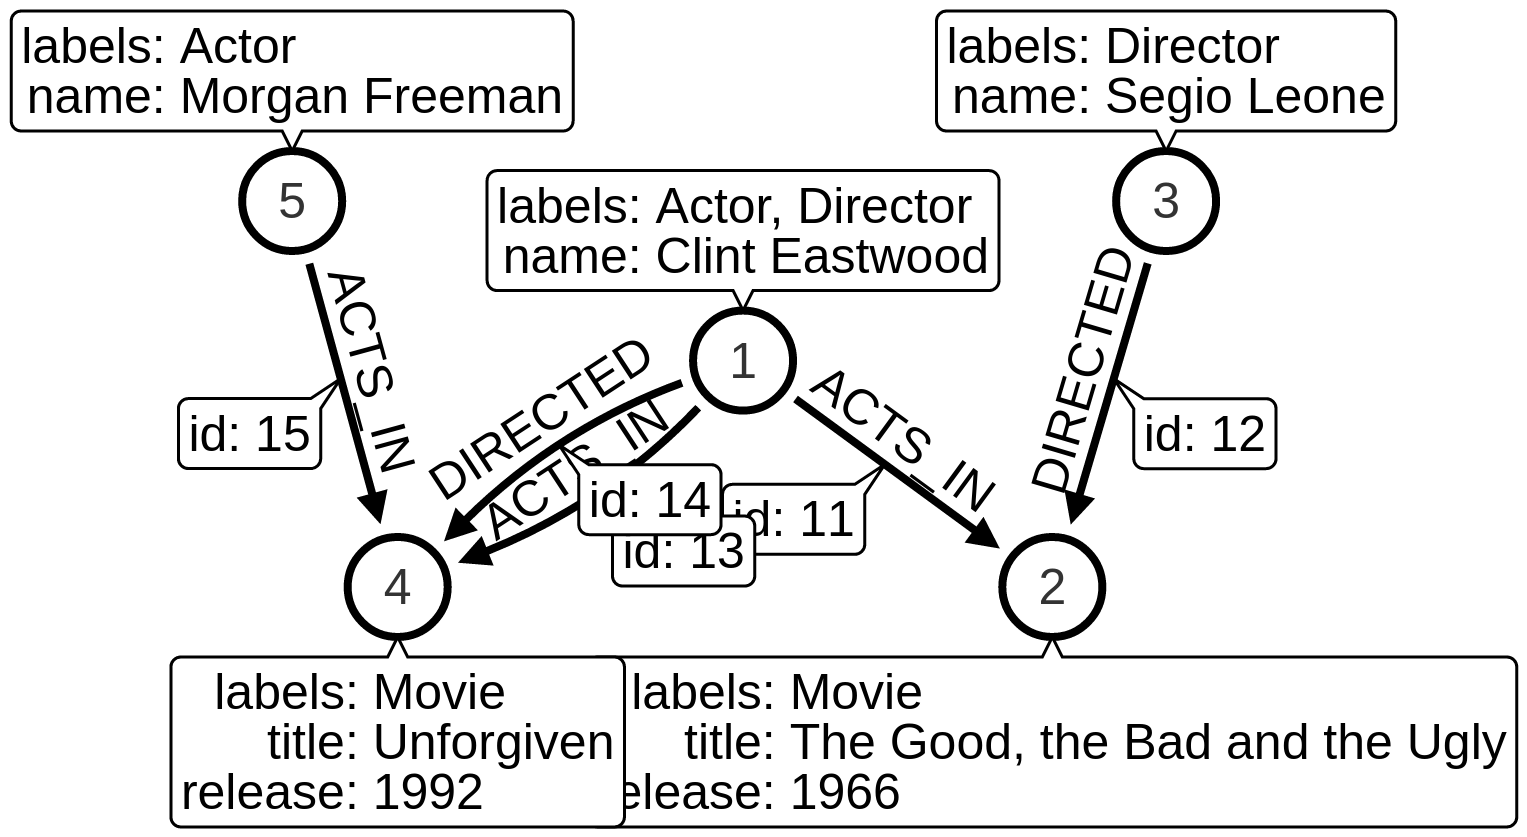
\includegraphics[width=6cm]{movie-graph}
	\captionof{figure}{Example movie graph.}
	\label{fig:running-example-property-graph}
\end{minipage}
\begin{minipage}[b]{0.53\linewidth}
	\footnotesize
	$V=\{1, 2, 3, 4, 5\}; E=\{11,12,13,14,15\};$
	
	$\verticestoedges(11) = \tuple{1, 2}; \verticestoedges(12) = \tuple{3, 2}; \ldots$

	$\vertexlabels = \{\atom{Actor}, \atom{Director}, \atom{Movie}\};$

	$\edgelabels = \{\atom{ACTS\_IN}, \atom{DIRECTED}\};$

	$\vertexlabelfunction(1) = \{\atom{Actor}, \atom{Director}\}; \vertexlabelfunction(2) = \{\atom{Movie}\}; \ldots;$

	$\edgelabelfunction(11) = \atom{ACTS\_IN}; \edgelabelfunction(12) = \atom{DIRECTED}; \ldots;$

	$\vertexproperties = \{\atom{name}, \atom{title}, \atom{release}\}; \edgeproperties = \{\};$

	$\propertyfunction{name}{1} = \atom{'Clint~Eastwood'}; \propertyfunction{name}{2} = \relnull; \ldots$

	$\propertyfunction{title}{1} = \relnull; \propertyfunction{title}{2} = \atom{'The~Good,~the~Bad~and~the~Ugly'}; \ldots$
	
	$\propertyfunction{release}{1} = \relnull; \propertyfunction{release}{2} = \atom{1966}; \ldots$
	\captionof{figure}{The dataset represented as a property graph.}
	\label{fig:property-graph-formalized}
\end{minipage}

In the context of this paper, we define a \emph{relation} as a bag (\emph{multiset}) of tuples: a tuple can occur more than once in the relation~\cite{DBLP:books/daglib/0020812}.
Given a property graph $G$, relation $r$ is a \emph{graph relation} if the following holds:
$$\forall A \in \attr{r}: \dom{A} \subseteq V \union E \union D,$$
where $\attr{r}$ is the set of attributes of $r$, $\dom{A}$ is the domain of attribute $A$. The schema of $r$, $\schema{r}$ is a list containing the attribute names. For schema transformations, the \appendtext operator is denoted by $\append$, the \removetext operator is denoted by $\remove$.

\subsection{Foundations of Relational Algebra}

\paragraph{Basic operators of relational algebra.} We give a brief summary of the operators in relational algebra. A more detailed discussion is available in database textbooks, \eg~\cite{DBLP:books/daglib/0006733}.

\paragraph{Unary operators.} The \projectiontext operator $\projectionop$ keeps a specific set of attributes in the relation: $ t = \projection{A_1, \ldots, A_n} \left(r\right).$ Note that the tuples are not deduplicated by default, \ie the results will have the same number of tuples as the input relation $r$. The projection operator can also rename the attributes, \eg $\projection{v1 \assign v2} \left(r\right)$ renames $\atom{v1}$ to $\atom{v2}$.
The \selectiontext operator $\selectionop$ filters the incoming relation according to some criteria. Formally,
$ t = \selection{\theta} \left(r\right), $
where predicate $\theta$ is a propositional formula. The operator selects all tuples in $r$ for which $\theta$ holds.

\paragraph{Binary operators.} The $\unionop$ operator produces the set union of two relations, while the $\bagunionop$ operator produces the \emph{bag union} of two operators, \eg $\{\tuple{1, 2}, \tuple{1, 2}, \tuple{3, 4}\} \bagunionop \{\tuple{1, 2}\} = \{\tuple{1, 2}, \tuple{1, 2}, \tuple{1, 2}, \tuple{3, 4}\}$. For both the \uniontext and \baguniontext operators, the schema of the operands must have the same number of attributes. Some authors also require that they share a common schema, \ie have the same set of attributes~\cite{DBLP:books/daglib/0020812}.

The $\cartesianproductop$ operator produces the \cartesianproducttext:

$$ t = r \cartesianproductop s.$$

The result of the \jointext operator $\joinop$ is determined by creating the Cartesian product of the relations, then filtering those tuples which are equal on the attributes that share a common name. The combined tuples are projected: from the attributes present in both of the two input relations, we only keep the ones in $r$ and drop the ones in $s$. Thus, the join operator is defined as
$$r \join s = \pi_{R \union S} \left(\selection{r.A_1 = s.A_1\,\land\,\ldots\,\land\,r.A_n = s.A_n)} \left(r \times s\right) \right),$$
where $ \{ A_1, \ldots, A_n \} $ is the set of attributes that occur both in $R$ and $S$, \ie $ R \intersection S = \{ A_1, \ldots, A_n \} $. Note that if the set of common attributes is empty, the \jointext operator is equivalent to the Cartesian product of the relations.
The join operator is both commutative and associative: $r \join s = s \join r$ and $(r \join s) \join t = r \join (s \join t)$, respectively.

The \antijointext operator $\antijoinop$ (also known as \emph{left anti semijoin}) collects the tuples from the left relation $r$ which have no matching pair in the right relation $s$:
$$ t = r \antijoin s = r \setminus \pi_{R} \left(r \join s\right), $$
where $\pi_{R}$ denotes a projection operator, which only keeps the attributes of the schema over relation $r$. The antijoin operator is not commutative and not associative.

The \leftouterjointext $\myleftouterjoin$ pads tuples from the left relation that did not match any from the right relation with $\relnull$ values and adds them to the result of the \jointext~\cite{DBLP:books/daglib/0015084}:
$$ t = r \myleftouterjoin s = (r \join s) \union (r \antijoin s) \cartesianproductop \{\relnull, \ldots, \relnull\}, $$

where the constant relation $\{\relnull, \ldots, \relnull\}$ is on the schema $S \setminus R$.

\subsection{Common Extensions to Relational Algebra}

Most textbooks also define \emph{extended operators} of relational algebra~\cite{DBLP:books/daglib/0020812}:

\begin{itemize}
	\item The \duplicateeliminationtext operator $\duplicateeliminationop$ eliminates duplicate tuples in a bag.
	\item The \groupingtext operator $\groupingop$ groups tuples according to their value in one or more attributes and aggregates the remaining attributes. %Aggregated values (scalars and inline collections) makes \rga not closed under \groupingtext.
	\item The \sorttext operator $\sortop$ transforms a bag relation of tuples to a list of tuples by ordering them. The ordering is defined by specified attributes of the tuples with an ordering direction (ascending $\asc$/descending $\desc$) for each attribute, \eg $\sortop_{\asc \atom{v1}, \desc \atom{v2}} (r)$.
\end{itemize}

The \toptext operator $\topp{l}{s}$ (adapted from~\cite{DBLP:conf/sigmod/LiCIS05}) takes a list as its input, skips the top $s$ tuples and returns the next $l$ tuples.\footnote{SQL implementations offer the \texttt{OFFSET} and the \texttt{LIMIT}/\texttt{TOP} keywords.}

\subsection{Graph-Specific Extensions to Relational Algebra}
\label{sec:rga}

We adapted graph-specific operators from~\cite{DBLP:conf/edbt/HolschG16}\footnote{The \textsc{GetNodes} operator introduced in~\cite{DBLP:conf/edbt/HolschG16} and did not support labels. We extended it by allowing the specification of vertex labels and renamed it to \getverticestext to be consistent with the rest of the definitions. We also extended the \textsc{ExpandIn} and \textsc{ExpandOut} operators to allow it to return a set of edges, and introduced the \expandbothtext operator to allow navigation to both directions.} and propose an additional operator.

The \getverticestext nullary operator $\getvertices{v}{t_1 \land \ldots \land t_n}$ returns a graph relation of a single attribute $v$ that contains the ID of all vertices that have \emph{all} of labels $t_1, \ldots, t_n$.

The \expandbothtext unary operator $\expandboth{E}{l_1 \lor \ldots \lor l_k \ast min \ldots max}{v}{w}{t_1 \land \ldots \land t_n}(r)$ adds (1)~a new attribute $w$ to $r$ containing the IDs of vertices having \emph{all} labels $t_1, \ldots, t_n$ that can be reached from vertices of attribute $v$ by traversing edges having \emph{any} labels $l_1, \ldots, l_n$, and (2)~a new attribute $E$ for the edges of the path from $v$ to $w$. The operator may use at least $\atom{min}$ and at most $\atom{max}$ hops, both defaulting to $1$ if omitted. % With the default setting, \ie $\atom{min}=\atom{max}=1$, a single edge variable $e$ can be used instead of edge list $E$.
The \expandintext operator~$\expandinop$ and \expandouttext operator~$\expandoutop$ only consider directed paths from $w$ to $v$ and from $v$ to $w$, respectively.

We propose the \alldifferenttext operator to guarantee the uniqueness of edges (see the remark on \emph{uniqueness of edges} in \autoref{sec:opencypher}). The \alldifferenttext operator $\alldifferent{E_1, E_2, E_3, \ldots}{(r)}$ filters $r$ to keep tuples where the variables in $\bigcup_{i} E_{i}$ are pairwise different.\footnote{Should e.g. $E_2$ be a set of the single variable $e_2$, the variable name can be used as a shorthand instead, so $\alldifferent{E_1, e_2, E_3, \ldots}{(r)} ~ \equiv ~ \alldifferent{E_1, \{e_2\}, E_3, \ldots}{(r)}$}
It can be expressed as a \selectiontext:
$$\alldifferent{E_1, E_2, E_3, \ldots}{(r)} = \selection{ \bigwedge\limits_{e_1, e_2 \,\in\, \bigcup\limits_{i} {E_i} ~ \wedge ~ { e_1 \,\neq\, e_2 } } { r.e_1 \,\neq\, r.e_2 } }{(r)}$$

\paragraph{Property access.} Assuming that $x$ is an attribute of a graph relation, we use the notation $x.a$ in (1)~attribute lists for projections and (2)~selection conditions to express the access to the corresponding value of property $a$ in the property graph~\cite{DBLP:conf/edbt/HolschG16}.

\paragraph{Summary.} \autoref{table:collections} provides an overview of the operators of \rga.

\newcommand{\propheader}{\multirow{2}{*}{\bf prop.}}
\newcommand{\rgaheader}{\multirow{2}{*}{\breakable{\bf RGA}}}

\setlength\tabcolsep{3.6pt}
\begin{table}[htb]
	\centering
	\begin{tabular}{||c||c|c|c||c|c|c||c||c||}
		\hline
		\multirow{2}{*}{\bf ops} &             \multirow{2}{*}{\bf operator}             &         \multirow{2}{*}{\bf name}         & \propheader & \multicolumn{3}{c||}{\bf output for} &             \multirow{2}{*}{\bf schema}              \\ \cline{5-7}
		&                                                       &                                           &             & \bf set & \bf bag &     \bf list     &  \\ \hline\hline
		\multirow{1}{*}{\bf 0}   &                  $\getvertices{v}{}$                  &             \getverticestext              &     set     &   set   &   set   &       set        &                  $\tuple{\atom{v}}$                  \\ \hline\hline %\cline{2-8}
%		&              $\getedges{v}{}{w}{}{e}{}$               &               \getedgestext               &     $-$     &   $-$   &   $-$   &       $-$        &               $\tuple{\atom{v, e, w}}$               \\ \hline\hline
		\multirow{8}{*}{\bf 1}   &         $\projection{v_1, v_2, \ldots} (r)$         &              \projectiontext              &      i      &   bag   &   bag   &       list       &         $\tuple{\atom{v_1, v_2, \ldots}}$          \\ \cline{2-8}
		&              $\selection{condition} (r)$              &              \selectiontext               &      i      &   set   &   bag   &       list       &                     $\schema{r}$                     \\ \cline{2-8}
		&            $\expandboth{v}{w}{}{e}{} (r)$             &              \expandbothtext              &     $-$     &   set   &   bag   &       list       &       $\schema{r} \append \tuple{\atom{e, w}}$       \\ \cline{2-8}
		&            $\alldifferent{variables} (r)$             &             \alldifferenttext             &      i      &   set   &   bag   &       list       &                     $\schema{r}$                     \\ \cline{2-8}
		&             $\duplicateeliminationop (r)$             &         \duplicateeliminationtext         &      i      &   set   &   set   &       list       &                     $\schema{r}$                     \\ \cline{2-8}
		&                     $\sort{\desc \atom{v_1}, \asc \atom{v_2}, \ldots} (r)$                     &                 \sorttext                 &      i      &  list   &  list   &       list       &                     $\schema{r}$                     \\ \cline{2-8}
		&          $\grouping{v_1, v_2, \ldots} (r)$          &               \groupingtext               &      i      &   set   &   set   &       set        &         $\tuple{\atom{v_1, v_2, \ldots}}$          \\ \cline{2-8}
		&                     $\topop (r)$                      &                 \toptext                  &     $-$     &  list   &  list   &       list       &                     $\schema{r}$                     \\ \hline\hline
		\multirow{5}{*}{\bf 2}   & $r \unionop s$, $r \minusop s$ & \uniontext, \minustext &     $-$     &   set   &   set   &       set        &                     $\schema{r}$                     \\ \cline{2-8}
		&                    $r \bagunion s$                    &               \baguniontext               &    c, a     &   bag   &   bag   &       bag        &                     $\schema{r}$                     \\ \cline{2-8}
		&               $r \cartesianproductop s$               &           \cartesianproducttext           &    c, a     &   set   &   bag   &       bag        &           $\schema{r} \append \schema{s}$            \\ \cline{2-8}
		&                    $r \joinop s$                      &                 \jointext                 &    c, a     &   set   &   bag   &       bag        & $\schema{r} \append (\schema{s} \minus \schema{r}) $ \\ \cline{2-8}
		&                $r \myleftouterjoin s$                 &            \leftouterjointext             &     $-$     &   set   &   bag   &       bag        & $\schema{r} \append (\schema{s} \minus \schema{r}) $ \\ \cline{2-8}
		&                   $r \antijoinop s$                   &               \antijointext               &    c, a     &   set   &   bag   &       bag        &                     $\schema{r}$                     \\ \cline{1-8}
	\end{tabular}
	\caption{Properties of relational graph algebra operators. A unary operator $\alpha$ is idempotent~(i), iff $\alpha(x) = \alpha(\alpha(x))$ for all inputs. A binary operator $\beta$ is commutative~(c), iff $x~\beta~y = y~\beta~x$ and associative~(a), iff $(x~\beta~y)~\beta~z = x~\beta~(y~\beta~z)$.}
	\label{table:collections}
\end{table}


\section{The openCypher Query Language}
\label{sec:opencypher}

\paragraph{Language.} As the primary query language of Neo4j~\cite{Neo4j}, Cypher~\cite{Cypher} was designed to read easily. It allows users to specify the graph pattern by a syntax resembling an actual graph. The goal of the \opencypher project~\cite{openCypher} is to provide a standardised specification of the Cypher language.
\cref{lst:example} shows an \opencypher query, which returns all people who (1)~are both actors and directors and (2)~have acted in a movie together with $\atom{Clint~Eastwood}$.

\begin{minipage}{\linewidth}
\begin{lstlisting}[label=lst:example, caption={Get people who are both actors and directors and acted in a movie with Clint Eastwood.}]
MATCH (a1)-[:ACTS_IN]->(:Movie)<-[:ACTS_IN]-(a2:Actor:Director)
WHERE a1.name = "Clint Eastwood"
RETURN a2
\end{lstlisting}
\end{minipage}

The query returns with a bag of vertices that have both the labels $\atom{Actor}$ and $\atom{Director}$ and share a common $\atom{Movie}$ neighbor through $\atom{ACTS\_IN}$ edges. Cypher guarantees that these edges are only traversed once, so the vertex of $\atom{Clint~Eastwood}$ is not returned (see the section on the uniqueness of edges).

\paragraph{Implementation.} While Neo4j uses a parsing expression grammar (PEG)~\cite{DBLP:conf/popl/Ford04} for specifying the grammar rules of Cypher, openCypher aims to achieve an implementation-agnostic specification by only providing a context-free grammar. The parser can be implemented using any capable parser technology, \eg \antlr~\cite{Parr:2013:DAR:2501720} or Xtext~\cite{DBLP:conf/oopsla/EysholdtB10}. %It also possible to generate a grammar following the ISO 14977 Extended Backus--Naur Form~\cite{ISO14977},

\paragraph{Legacy grammar rules.} It is not a goal of the openCypher project to fully cover the features of Neo4j's Cypher language: ``Not all grammar rules of the Cypher language will be standardised in their current form, meaning that they will not be part of openCypher as-is. Therefore, the openCypher grammar will not include some well-known Cypher constructs; these are called 'legacy'.''\footnote{\url{https://github.com/opencypher/openCypher/tree/master/grammar}} The \emph{legacy rules} include commands (\lstinline+CREATE INDEX+, \lstinline+CREATE UNIQUE CONSTRAINT+, etc.), pre-parser rules (\lstinline+EXPLAIN+, \lstinline+PROFILE+) and deprecated constructs (\lstinline+START+). A detailed description is provided in the openCypher specification. In our work, we focused on the \emph{standard core} of the language and ignored legacy rules.

% http://neo4j.com/docs/developer-manual/current/cypher/#cypherdoc-uniqueness
\paragraph{Uniqueness for edges.} In an \opencypher query, a \lstinline+MATCH+ clause defines a graph pattern. A query can be composed of multiple patterns spanning multiple \lstinline+MATCH+ clauses. For the matches of a pattern within a single \lstinline+MATCH+ clause, edges are required to be unique. %even for disconnected graph patterns.
However, matches for multiple \lstinline+MATCH+ clauses can share edges. This uniqueness criterium can be expressed in a compact way with the \alldifferenttext operator introduced in \cref{sec:rga}. For vertices, this restriction does not apply.

\paragraph{Aggregation.} It indeed makes sense to calculate aggregation over graph pattern matches, though, its result will not necessarily be pattern match with vertices and edges. Based on some \emph{grouping criteria}, matches are put into categories, and values for the grouping criteria as well as grouping functions\footnote{For example, \lstinline+count+, \lstinline+avg+, \lstinline+sum+, \lstinline+max+, \lstinline+min+, \lstinline+stdDev+, \lstinline+stdDevP+, \lstinline+collect+. The \lstinline+collect+ function is an exception as it does not return a single scalar value but returns a collection (list).} over the groups, the aggregations are evaluated in a single tuple for each and every category. In the SQL query language, grouping criteria is explicitly given by using the \lstinline+GROUP BY+ clause. In \opencypher, however, this is done implicitly in the \lstinline+RETURN+ as well as in \lstinline+WITH+ clauses: vertices, edges and their properties that appear outside the grouping functions become the \emph{grouping criteria}.\footnote{This approach is also used by some SQL code assistant IDEs generating the \lstinline+GROUP BY+ clause for a query.}

\paragraph{Subqueries.} One can compose an \opencypher query of multiple subqueries. Subqueries, written subsequently, mostly begin by a \lstinline+MATCH+ clause and end at (including) a \lstinline+RETURN+ or \lstinline+WITH+ clause, the latter having an optional \lstinline+WHERE+ clause to follow. The \lstinline+WITH+ and \lstinline+RETURN+ clauses determine the resulting schema of the subquery by specifiying the vertices, edges, attributes and aggregates of the result. When \lstinline+WITH+ has the optional \lstinline+WHERE+ clause, it applies an other filter on the subquery result.~\footnote{This is much like the \lstinline+HAVING+ construct of the SQL language with the major difference that it is also allowed in \opencypher in case no aggregation has been done.} The last subquery must be ended by \lstinline+RETURN+, whereas all the previous ones must be ended by \lstinline+WITH+. If a query is composed by more than one subqueries, their results are joined together using \jointext or \leftouterjointext operators.


\section{Mapping \opencypher Queries to \RGA}
\label{sec:compilation}

In this section, we first give the mapping algorithm of \opencypher queries to \rga, then we give a more detailed listing of the compilation rules for the query language constructs in \autoref{table:mapping}.
We follow the bottom-up approach to build the \rga tree based on the \opencypher query. The algorithm is as follows. Join operations always use all common variables to match the two inputs (see \jointext in \autoref{sec:rga}).

\setlength\tabcolsep{3.6pt}
\begin{enumerate}
\label{alg:build-rga-tree}
	\item A single pattern is turned left-to-right to a \getverticestext for the first vertex and a chain of \expandintext, \expandouttext or \expandbothtext operators for inbound, outbound or undirected relationships, respectively.
	\item Patterns in the same \lstinline+MATCH+ clause are joined by \jointext.
	\item Append an \alldifferenttext operator for all edge variables that appear in the \lstinline+MATCH+ clause because of the non-repeating edges language rule.
	\item Process the \lstinline+WHERE+ clause. Note that according to the grammar, \lstinline+WHERE+ is bound to a \lstinline+MATCH+ clause.
	\item Several \lstinline+MATCH+ clauses are connected to a left deep tree of \jointext. If \lstinline+MATCH+ has the \lstinline+OPTIONAL+ modifier, \leftouterjointext is used instead of \jointext.
	\item If there is a positive or negative pattern deferred from \lstinline+WHERE+ processing,
		append it as a \jointext or \antijointext operator, respectively.
	\item Append \groupingtext, if \lstinline+RETURN+ or \lstinline+WITH+ clause has grouping functions inside
	\item Append \projectiontext operator based on the \lstinline+RETURN+ or \lstinline+WITH+ clause. This operator will also handle the renaming (i.e. \lstinline+AS+).
	\item Append \duplicateeliminationtext operator, if the \lstinline+RETURN+ or \lstinline+WITH+ clause has the \lstinline+DISTINCT+ modifier.
	\item Append a \selectiontext operator in case the \lstinline+WITH+ had the optional \lstinline+WHERE+ clause.
	\item If this is not the first subquery, join to the \rga tree using \jointext or \leftouterjointext.
	\item Assemble a \uniontext operation from the query parts\footnote{In this context, query parts refer to those parts of the query connected by the \lstinline+UNION+ \opencypher keyword.}. As the \uniontext operator is technically a binary operator, the \uniontext of more than two query parts are represented as a left deep tree of \lstinline+UNION+ operators.
\end{enumerate}

\setlength\extrarowheight{2.5pt}
\setlength\tabcolsep{3.6pt}
\begin{table}[htbp]
	\centering
	\begin{tabular}{|l|l|l|}
		\hline
		\multicolumn{2}{|l|}{ \bf Language construct } & \bf Relational algebra expression \\ \hline\hline

		%\hline
		\multicolumn{3}{|l|}{Vertex, edge and path patterns } \\ \cline{2-3}

		& \lstinline+()+ & $\getvertices{\_v}{}$ \\ \cline{2-3}

		& \lstinline+(:types)+ & $\getvertices{\_v}{types}$ \\ \cline{2-3}

		& \lstinline+(<v>v</v>:types)+ & $\getvertices{v}{types}$ \\ \cline{2-3}

		% expand operators
		& \lstinline+<v>p</v>-[<v>e</v>:<v>labels</v>]-(<v>w</v>:types...)+ & \multirow{2}{*}{$\expandboth{v}{w}{types}{e}{labels}{1}{1} (\atom{p})$} \\ \cline{2-2}

		& \lstinline+<v>p</v><-[<v>e</v>:<v>labels</v>]->(<v>w</v>:types...)+ & \\ \cline{2-3}

		& \lstinline+<v>p</v>-[<v>e</v>:<v>labels</v>]->(<v>w</v>:types...)+ & $\expandout{v}{w}{types}{e}{labels}{1}{1} (\atom{p})$ \\ \cline{2-3}

		& \lstinline+<v>p</v><-[<v>e</v>:<v>labels</v>]-(<v>w</v>:types...)+ & $\expandin{v}{w}{types}{e}{labels}{1}{1} (\atom{p})$ \\ \cline{2-3}

		& \lstinline+<v>p</v>-[<v>E</v>:<v>labels</v>*<v>min</v>..<v>max</v>]->(<v>w</v>:<v>t2</v>)+ & $\expandout{v}{w}{types}{E}{labels}{min}{max}(\atom{p})$ \\ \cline{2-3}

		& \lstinline+<v>p</v>-[<v>E</v>:<v>labels</v>*]->(<v>w</v>:<v>t2</v>)+ & $\transitiveclosureout{v}{w}{types}{E}{labels}(\atom{p})$ \\ \cline{2-3}

		\hline \multicolumn{3}{|l|}{Combining and filtering pattern matches } \\ \cline{2-3}

		& \lstinline+MATCH <v>p</v>+ & $\alldifferent{\atom{edges~of~p}} \left(\atom{p}\right)$ \\ \cline{2-3}

		& \lstinline+MATCH <v>p1</v>, <v>p2</v>+ &
		$\alldifferent{\atom{edges~of~p1~and~p2}} \left( \atom{p_1}~\join~\atom{p_2} \right)$ \\ \cline{2-3}

		& \breakable{
			\lstinline+MATCH <v>p1</v>+ \\
			\lstinline+MATCH <v>p2</v>+
		} &
		$\alldifferent{\atom{edges~of~p1}} \left(\atom{p_1}\right)~\join~\alldifferent{\atom{edges~of~p2}} \left(\atom{p_2}\right)$ \\ \cline{2-3}

		& \breakable{
			\lstinline+MATCH <v>p1</v>+ \\
			\lstinline+OPTIONAL MATCH <v>p2</v>+
		} & $\alldifferent{\atom{edges~of~p1}} \left(\atom{p_1}\right)~\myleftouterjoin~\alldifferent{\atom{edges~of~p2}} \left(\atom{p_2}\right)$ \\ \cline{2-3}

		& \breakable{
			\lstinline+MATCH <v>p</v>+ \\
			\lstinline+WHERE <v>condition</v>+
		} & \breakable{$\selection{\atom{condition}}{\left( r \right)}$, where $\atom{condition}$ may \tabularnewline specify patterns and arithmetic \tabularnewline constraints on existing variables} \\ \cline{2-3}

		\hline \multicolumn{3}{|l|}{Result and sub-result operations. Rules for \lstinline+RETURN+ also apply to \lstinline+WITH+.} \\ \cline{2-3}

		& \lstinline+RETURN <v>variables</v>+ & $\projection{\atom{variables}}{\left( r \right)}$ \\ \cline{2-3}

		& \lstinline+RETURN <v>v1</v> AS <v>alias1</v> ...+ & $\projection{\atom{v1} \assign \atom{alias1}, \ldots }\left( r \right)$ \\ \cline{2-3}

		& \lstinline+RETURN DISTINCT <v>variables</v>+ & $\duplicateelimination\left(\projection{\atom{variables}}{\left( r \right)}\right)$ \\ \cline{2-3}

		& \lstinline+RETURN <v>variables</v>, <v>aggregates</v>+ & $\grouping{\atom{variables}, \atom{aggregates}}{\left( r \right)}$ \\ \cline{2-3}

		\hline \multicolumn{3}{|l|}{List operations } \\ \cline{2-3}

		& \lstinline+ORDER BY <v>v1</v> [ASC|DESC] ...+ & $\sort{\asc/\desc \atom{v1}, \ldots}{\left( r \right)}$ \\ \cline{2-3}

		& \lstinline+LIMIT <v>l</v>+ & $\limit{l}(r)$ \\ \cline{2-3}

		& \lstinline+SKIP <v>s</v>+ & $\skipp{s}(r)$ \\ \cline{2-3}

		& \lstinline+SKIP <v>s</v> LIMIT <v>l</v>+ & $\topp{l}{s}(r)$ \\ \cline{2-3}

		\hline \multicolumn{3}{|l|}{Combining results } \\ \cline{2-3}

		& \lstinline+<v>query1</v> UNION <v>query2</v>+ & $r_1 \union r_2$ \\ \cline{2-3}

		& \lstinline+<v>query1</v> UNION ALL <v>query2</v>+ & $r_1 \bagunion r_2$ \\ \hline
	\end{tabular}
	\caption{Mapping from \opencypher constructs to relational algebra.}
	\label{table:mapping}
\end{table}

\paragraph{Example.} The example query in~\autoref{lst:example} can be formalized as:
{\footnotesize
	\begin{align*}
	&\projection{a2} \Bigg(\selection{a1.name = 'C.\,E.'} \Big( \alldifferent{\_e1, \_e2} \expandin{a1}{a2}{Actor \land Director}{\_e1}{ACTS\_IN}{1}{1} \expandout{a1}{}{Movie}{\_e2}{ACTS\_IN}{1}{1} \left(\getvertices{a1}{Actor}\right) \Big) \Bigg)
	\end{align*}
}

Note that the $\alldifferentop$ guarantees the uniqueness constraint for the edges (\autoref{sec:opencypher}), which prevents the query from returning the vertex $\atom{Clint~Eastwood}$.

\paragraph{Optimisations.} Queries with negative conditions for patterns can also be expressed using the \antijointext operator. For example, \lstinline+MATCH <v>p1</v> WHERE NOT <v>p2</v>+ can be formalized as
$$\alldifferent{\atom{edges~of~p1}} \left(\atom{p_1}\right) \antijoin \alldifferent{\atom{edges~of~p2}} \left(\atom{p_2}\right)$$

\paragraph{Limitations.} Our mapping does not completely cover the \opencypher language. As discussed in \autoref{sec:opencypher}, some constructs are defined as legacy and thus were omitted. Also, we did not formalize expressions (\eg  conditions in selections), collections (arrays and maps), which are required for both path variables\footnote{\lstinline+MATCH p=(:Person)-[:FRIEND*1..2]->(:Person)+} and the \lstinline+UNWIND+ operator. The mapping does not cover parameters and data manipulation operations, \eg \lstinline+CREATE+, \lstinline+DELETE+, \lstinline+SET+ and \lstinline+MERGE+.


\section{Related Work}
\label{sec:related-work}

The TinkerPop framework~\cite{TinkerPop} aims to provide a standard data model for property graphs, along with Gremlin, a high-level graph-traversal language~\cite{Rodriguez:2015:GGT:2815072.2815073} and the Gremlin Structure API, a low-level programming interface.

Besides property graphs, graph queries can be formalized on different graph-like data models and even relational databases.

\paragraph{EMF.} The Eclipse Modeling Framework (EMF) is an object-oriented modelling framework widely used in model-driven engineering. 
Henshin~\cite{DBLP:conf/models/ArendtBJKT10} provides a visual language for defining patterns, while Epsilon~\cite{DBLP:conf/icmt/KolovosPP08} and \viatraquery~\cite{DBLP:conf/models/BergmannHRVBBO10} provide high-level declarative (textual) query languages, Epsilon Pattern Language and \vql.

\paragraph{RDF.} The Resource Description Framework (RDF)~\cite{RDF} aims to describe entities of the semantic web. RDF assumes sparse, ever-growing and incomplete data stored as triples that can be queried using the \sparql~\cite{SPARQL} graph pattern language.
%A formal definition of the \sparql language is given in~\cite{DBLP:journals/tods/PerezAG09}.

\lstset{language=}

\paragraph{SQL.} In general, relational databases offer limited support for graph queries: recursive queries are supported by \mbox{PostgreSQL} using the \lstinline+WITH RECURSIVE+ keyword and by the Oracle Database using the \lstinline+CONNECT BY+ keyword. Graph queries are supported in \saphana Graph
Scale-Out Extension prototype~\cite{DBLP:conf/btw/RudolfPBL13}, through a SQL-based language~\cite{DBLP:conf/gg/KrauseJDSKN16}.


\section{Conclusion and Future Work}
\label{sec:conclusion}

In this paper, we presented a formal specification for a subset of the \opencypher query language. This provides the theoretical foundations to use \opencypher as a language for graph query engines. Using the proposed mapping, an \opencypher-compliant query engine could be built on any relational database engine to (1)~store property graphs as graph relations and to (2)~efficiently evaluate the extended operators of \rga.

As a future work, we will give formal specification of the operators for incremental query evaluation, which requires us to define \emph{maintenance operations} to keep their result in sync with the latest set of changes. Our long-term research objective is to design and prototype a \emph{distributed, incremental graph query engine}~\cite{DBLP:conf/models/SzarnyasIRHBV14} for the property graph data model.



% !TeX spellcheck = en_GB
% !TeX encoding = UTF-8
\chapter{Incremental Query Evaluation}
\label{chp:incremental}

This chapter is based on our paper~\cite{PerPol2017Incremental}.

In many use cases, queries are continuously evaluated, while the data only changes rarely and to a small degree. The validation queries in MDE are a typical example of such a workload. The goal of \emph{incremental query evaluation} is to speed up such queries, using the (partial) results obtained during the previous executions of the query and only computing the effect of the latest set of changes.

Incremental query evaluation algorithms typically
use additional data structures for caching interim results. This implies that they usually consume more memory than non-incremental, search-based algorithms. In other words, they trade memory consumption for execution speed. This approach, called \emph{space--time tradeoff}, is well-known and widely used in computer science.

Numerous algorithms were proposed for incremental pattern matching. Mostly, these algorithms originate from the field of rule-based expert systems. In this paper, we use the \emph{Rete algorithm}~\cite{DBLP:journals/ai/Forgy82}, which creates a \emph{data flow network} for evaluating relational queries. %~\cite{DBLP:journals/ai/Forgy82}. %, which creates  The network stores the partial matches found in the graph. %The \emph{TREAT algorithm}~\cite{Miranker:1991:OPT:627280.627434} aims to minimize memory usage, while having the same algorithmic complexity as Rete. It stores only the input facts and the conflict sets, and does not store partial pattern matches. Another candidate is the \emph{LEAPS algorithm}~\cite{Batory:1994:LA:899216}, which is claimed to provide better space--time complexity. However, we found that LEAPS is difficult to understand and implement even on a single workstation, not to mention the distributed case.

%Rete has many improved versions (\eg Rete II, Rete III, Rete-NT), however, unlike the original algorithm, these are not publicly available. In this paper, we discuss the Rete algorithm, one of the most used incremental pattern matching algorithms. Experimenting with improved versions or alternative approaches is subject to future work.

\section{Overview of Rete Networks}
\label{sec:rete}

%\fig{rete/rete}{The structure of the Rete propagation network}{0.65}
\todo{Draw a Rete network in tikz}

The Rete algorithm constructs a network of three types of nodes. Following \autoref{fig:rete/rete}, from bottom to top:

\begin{enumerate}
	\item \emph{Input nodes} are responsible for indexing the graph, \ie they store the appropriate tuples for vertices and edges in the graph. They are also responsible for sending \emph{change sets} as \emph{update messages} to worker nodes that are \emph{subscribed} to them.
	\item \emph{Worker nodes} perform a relational algebraic operation on their input and propagate the results to other worker nodes or production nodes. Some worker nodes are \emph{stateful}: they store partial query results in their memory to allow incremental reevaluation.
	Worker nodes have two types: \emph{unary nodes} have a single input slot, \emph{binary nodes} have two input slots.
	\item \emph{Production nodes} are terminators that provide an interface for fetching the results.
\end{enumerate}

The Rete network operates as follows. First, the network computes the set of pattern matches in the graph. Then upon a change in the graph, the network is incrementally maintained by propagating \emph{update messages} (also known as \emph{deltas}, denoted with the $\Delta$ character). Adding new graph matches to the result set is expressed as \emph{positive update messages}, while removing matches results in \emph{negative update messages}.

%\section{Rete Nodes}

In the following, we discuss Rete nodes in detail. For unary and binary nodes, we formulate the \emph{maintenance operations}, which are performed upon receiving an update message. For these operations, we denote the output relation by $t$, the updated output relation by $t'$, and the propagated update message on the output by $\Delta t$. If the \emph{propagated update message} is a positive update, $t' = t \cup \Delta t$, if it is a negative update, $t' = t \setminus \Delta t$.

\section{Input Nodes}

%\fig{rete/input-node}{Graphical notation of an input node}{\retescale}

\emph{Input nodes} %(\autoref{fig:rete/input-node})
provide the relations for each label of the graph. For example, the input node for the $\mathsf{requires}$ edge label of example the graph (\autoref{fig:trainbenchmark-instance-model}) returns tuples that are currently in the $\mathit{requires}$ relation: $ \left\{ \tuple{2, d, 6}, \tuple{4, f, 7} \right\} $. This input node is also responsible for propagating changes to worker nodes in the network:

\begin{itemize}
	\item If a $\mathsf{requires}$ edge `t' is inserted from vertex 2 to 5, the input node sends a positive update message to its subscriber nodes with the change set $ \left\{ \tuple{2, t, 4} \right\} $.
	\item If the edge `d' between vertices 2 and 6 is deleted, the input node sends a negative update to its subscriber nodes with the change set $ \left\{ \tuple{2, d, 6} \right\} $.
\end{itemize}

The relations contained by input nodes can be defined with nullary operators (\autoref{sec:nullary}): input nodes indexing vertices implement the \getverticestext operator, while input nodes indexing edges implement the \getedgestext operator.

\section{Unary Nodes}

%\fig{rete/unary-node}{Graphical notation of a unary node}{\retescale}

\emph{Unary nodes} %(\autoref{fig:rete/unary-node})
have one input slot. They filter or transform the tuples of the parent node according to certain criteria. In the following, the relation representing the input tuples is denoted with $r$, the relation representing the output tuples is denoted with $t$, and the operator processing the input is denoted with $\alpha$:
\begin{align*}
t = \op{\alpha}{r}.
\end{align*}

\subsubsection{Maintenance}

In the following, we assume that the $\alpha$ operator is \emph{distributive} \wrt the union ($\union$) and set minus ($\setminus$) operators. If a unary node receives an update $\Delta r$, it performs the operation and computes the change set. For \emph{positive updates}, the result ($t'$) and the changeset ($\Delta t$) are:
\begin{align*}
	t'       & \equiv \op{\alpha}{r \union \Delta r} \\
			 & = \op{\alpha}{r} \union \op{\alpha}{\Delta r} \\
			 & = t \union \underbrace{\op{\alpha}{\Delta r}}_{\Delta t} \\
\end{align*}

Similarly, for \emph{negative updates}:
\begin{align*}
	t'       & \equiv \op{\alpha}{r \setminus \Delta r} \\
			 & = \op{\alpha}{r} \setminus \op{\alpha}{\Delta r} \\
			 & = t \setminus \underbrace{\op{\alpha}{\Delta r}}_{\Delta t}
\end{align*}

Unary nodes are often implemented as \emph{stateless} nodes, \ie they do not store the results of the previous executions. Instead, these results are cached in their subscribers, \eg indexers of \emph{binary nodes} (\autoref{sec:binary-nodes}) or \emph{production nodes} (\autoref{sec:production-node}).

As their name suggests, unary nodes implement unary relational algebraic operators (\autoref{sec:unary}):

\begin{itemize}
	\item The \emph{projection node} performs a projection operation on the input relation.
	\item The \emph{selection node} performs a selection operation on the input relation.
\end{itemize}

As both the projection and the selection operators are distributive \wrt the union and set minus operators, their results can be maintained by performing the operation for the change set $\Delta r$.

\section{Binary Nodes}
\label{sec:binary-nodes}

%\fig{rete/binary-node}{Graphical notation of a binary node}{\retescale}

\emph{Binary nodes} %(\autoref{fig:rete/binary-node})
have two input slots: the \emph{primary} ($p$) and the \emph{secondary} ($s$). Binary node implementations typically cache both their input relations in \emph{indexers}.

\subsection{Natural Join Node}

\subsubsection{Maintenance}

In the following, we define the maintenance operations for natural join nodes. If a natural join node receives a \emph{positive update} $\Delta p$ on its \emph{primary} input slot, the result ($t'$) and the change set ($ \Delta t$) are determined as follows:
\begin{align*}
	t'       & \equiv \left(p \cup \Delta p\right) \join s           \\
	         & = (p \join s) \union (\Delta p \join s) \\
	         & = t \union \underbrace{(\Delta p \join s)}_{\Delta t}
\end{align*}

If the node receives a \emph{positive update} $\Delta s$ on its \emph{secondary} input slot, the result ($t'$) and the change set ($ \Delta t$) are the following:
\begin{align*}
	t'       & \equiv p \join \left(s \cup \Delta s\right)           \\
	         & = (p \join s) \union (p \join \Delta s) \\
	         & = t \union \underbrace{(p \join \Delta s)}_{\Delta t}
\end{align*}

For \emph{negative updates}, the changeset is the same, but it is propagated as a \emph{negative update}. The result is $t' = t \setminus (\Delta p \join s)$ and $t' = t \setminus (p \join \Delta s)$, for updates messages on the primary and the secondary input slots, respectively.

\subsection{Antijoin Node}

\subsubsection{Maintenance}

As the antijoin operator is not commutative, handling update messages requires us to distinguish between the following cases:

\begin{itemize}
	\item Update on the primary slot.
	\begin{itemize}
		\item Positive update: send a \emph{positive update} for each incoming tuple for which there is no match on the secondary indexer.
		\begin{align*}
			t'       & \equiv \left(p \cup \Delta p\right) \antijoin s               \\
			         & = (p \antijoin s) \union (\Delta p \antijoin s) \\
			         & = t \union \underbrace{(\Delta p \antijoin s)}_{\Delta t}
		\end{align*}

		\item Negative update: send a \emph{negative update} with the following tuples:
		$$ \Delta t = \Delta p \antijoin s $$
	\end{itemize}

	\item Update on the secondary slot. This case is more difficult to handle, so we recall the definition of the antijoin operator from \autoref{sec:binary} for relations $p$ and $s$:
	\begin{align*}
		t & \equiv p \antijoin s = p \setminus \left(p \join \pi_{P \cap S} (s)\right),
	\end{align*}




	%t & \equiv p \antijoin s \\
	%&= p \setminus \pi_{P} \left(p \join s\right),

	\begin{itemize}
		\item For positive updates, the result set can be expressed as:
		\begin{align*}
			t'       & \equiv p \antijoin \left(s \cup \Delta s\right) \\
			         & = p \setminus \left( p \join \pi_{P \cap S} \left(s \cup \Delta s\right) \right)
		\end{align*}

		Positive updates on the secondary indexer result in \emph{negative updates} on the result set, so that $t' = t \setminus \Delta t$, hence $\Delta t = t \setminus t'$.

		For sets $A, B \subseteq C$, the following equality holds: $(C \setminus A) \setminus (C \setminus B) = B \setminus A$.
		Applying this with $C = p$ and using the distributive property of the natural join operator, the change set can be determined as:
		\begin{align*}
		\Delta t = t \setminus t' & = \overbrace{\left[p \setminus \left(p \join \pi_{P \cap S} (s)\right)\right]}^{t} \setminus \overbrace{\left[p \setminus \left( p \join \pi_{P \cap S} \left(s \cup \Delta s\right) \right)\right]}^{t'} \\
		         & = \left( p \join \pi_{P \cap S} \left(s \cup \Delta s\right) \right) \setminus \left(p \join \pi_{P \cap S} (s)\right) \\
		         & = p \join \left(\pi_{P \cap S} (s \cup \Delta s) \setminus \pi_{P \cap S} (s) \right) \\
		         & = p \join \left(\pi_{P \cap S} (s) \cup \pi_{P \cap S} (\Delta s) \setminus \pi_{P \cap S} (s) \right) \\
		         & = p \join \left(\pi_{P \cap S} (\Delta s) \setminus \pi_{P \cap S} (s) \right)
		\end{align*}

		\item For negative updates, the result set can be expressed as:
		\begin{align*}
		t' & \equiv p \antijoin \left(s \setminus \Delta s\right) \\
		   & = p \setminus \left(p \join \pi_{P \cap S} \left(s \setminus \Delta s\right)\right),
		\end{align*}

		Negative updates may result in \emph{positive updates} on the result set. Since $t' = t \union \Delta t$, we can define $\Delta t = t' \setminus t$:
		\begin{align*}
		\Delta t = t' \setminus t & = \overbrace{\left[p \setminus \left( p \join \pi_{P \cap S} \left(s \setminus \Delta s\right) \right)\right]}^{t'} \setminus \overbrace{\left[p \setminus \left(p \join \pi_{P \cap S} (s)\right)\right]}^{t} \\
		         & = \underbrace{\left(p \join \pi_{P \cap S} (s)\right)}_{x} \setminus \underbrace{\left( p \join \pi_{P \cap S} \left(s \setminus \Delta s\right) \right)}_{y}
		\end{align*}
		Although this change set may seem difficult to calculate, we point out that both $x$ and $y$ can be maintained incrementally. Furthermore, they only grow linearly in the size of $p$, as the join operator does not introduce new attributes, hence it can only reduce the number of elements in the relation.
	\end{itemize}
\end{itemize}

\subsection{Union Node}

\begin{align*}
	t' & \equiv (p \union \Delta p) \union s \\
	   & = (p \union s) \union \Delta p \\
	   & = t \union \underbrace{\Delta p}_{\Delta t}
\end{align*}

As the union operator is commutative, for updates on the secondary input, the rules are the same, but $p$ and $s$ are changed and $\Delta p$ is renamed to $\Delta s$.

\section{Production Nodes}
\label{sec:production-node}

\emph{Production nodes} are terminators that provide an interface for fetching results of a query (the match set) and also propagate the changes introduced by the latest update message.\footnote{In popular Rete implementations, clients are usually subscribed to the production nodes and notified about the changes in the result set.}

\subsubsection{Maintenance}

The change set is defined as:
$$\Delta t \equiv \bigunion_{i=1}^{n} \Delta r_i,$$

where $\Delta r_1, \Delta r_2, \ldots, \Delta r_n$ are the update messages triggered by the last change.
%For positive update messages, $t' = t \union \Delta t,$ while for negative update messages $t' = t \setminus \Delta t.$


\bibliographystyle{abbrv}
\bibliography{bib}

\IfFileExists{./disable-appendix}{
	% do nothing
}{
	\appendix
	\chapter{TCK Acceptance Tests}
\label{chp:tck}

\section{AggregationAcceptance}

\subsection{Support multiple divisions in aggregate function}

\subsubsection*{Query specification}

\begin{lstlisting}
MATCH (n)
RETURN count(n) / 60 / 60 AS count
\end{lstlisting}

\subsubsection*{Relational algebra expression}

\begin{flalign*}
& \text{Cannot convert to expression.} &
\end{flalign*}

\subsubsection*{Relational algebra tree}

\text{Cannot visualize tree.}

\subsubsection*{Relational algebra tree for incremental queries}

Cannot visualize incremental tree.
\subsection{Support column renaming for aggregates as well}

\subsubsection*{Query specification}

\begin{lstlisting}
MATCH ()
RETURN count(*) AS columnName
\end{lstlisting}

\subsubsection*{Relational algebra expression}

\begin{flalign*}
& \text{Cannot convert to expression.} &
\end{flalign*}

\subsubsection*{Relational algebra tree}

\text{Cannot visualize tree.}

\subsubsection*{Relational algebra tree for incremental queries}

Cannot visualize incremental tree.
\subsection{Aggregates inside normal functions}

\subsubsection*{Query specification}

\begin{lstlisting}
MATCH (a)
RETURN size(collect(a))
\end{lstlisting}

\subsubsection*{Relational algebra expression}

\begin{flalign*}
& \text{Cannot convert to expression.} &
\end{flalign*}

\subsubsection*{Relational algebra tree}

\text{Cannot visualize tree.}

\subsubsection*{Relational algebra tree for incremental queries}

Cannot visualize incremental tree.
\subsection{Handle aggregates inside non-aggregate expressions}

\subsubsection*{Query specification}

\begin{lstlisting}
MATCH (a {name: 'Andres'})<-[:FATHER]-(child)
RETURN {foo: a.name='Andres', kids: collect(child.name)}
\end{lstlisting}

\subsubsection*{Relational algebra expression}

\begin{flalign*}
& \text{Cannot convert to expression.} &
\end{flalign*}

\subsubsection*{Relational algebra tree}

\text{Cannot visualize tree.}

\subsubsection*{Relational algebra tree for incremental queries}

Cannot visualize incremental tree.
\subsection{Count nodes}

\subsubsection*{Query specification}

\begin{lstlisting}
MATCH (a:L)-[rel]->(b)
RETURN a, count(*)
\end{lstlisting}

\subsubsection*{Relational algebra expression}

\begin{flalign*}
& \text{Cannot convert to expression.} &
\end{flalign*}

\subsubsection*{Relational algebra tree}

\text{Cannot visualize tree.}

\subsubsection*{Relational algebra tree for incremental queries}

Cannot visualize incremental tree.
\subsection{Sort on aggregate function and normal property}

\subsubsection*{Query specification}

\begin{lstlisting}
MATCH (n)
RETURN n.division, count(*)
ORDER BY count(*) DESC, n.division ASC
\end{lstlisting}

\subsubsection*{Relational algebra expression}

\begin{flalign*}
& \text{Cannot convert to expression.} &
\end{flalign*}

\subsubsection*{Relational algebra tree}

\text{Cannot visualize tree.}

\subsubsection*{Relational algebra tree for incremental queries}

Cannot visualize incremental tree.
\subsection{Aggregate on property}

\subsubsection*{Query specification}

\begin{lstlisting}
MATCH (n)
RETURN n.x, count(*)
\end{lstlisting}

\subsubsection*{Relational algebra expression}

\begin{flalign*}
& \text{Cannot convert to expression.} &
\end{flalign*}

\subsubsection*{Relational algebra tree}

\text{Cannot visualize tree.}

\subsubsection*{Relational algebra tree for incremental queries}

Cannot visualize incremental tree.
\subsection{Count non-null values}

\subsubsection*{Query specification}

\begin{lstlisting}
MATCH (n)
RETURN n.y, count(n.x)
\end{lstlisting}

\subsubsection*{Relational algebra expression}

\begin{flalign*}
& \text{Cannot convert to expression.} &
\end{flalign*}

\subsubsection*{Relational algebra tree}

\text{Cannot visualize tree.}

\subsubsection*{Relational algebra tree for incremental queries}

Cannot visualize incremental tree.
\subsection{Sum non-null values}

\subsubsection*{Query specification}

\begin{lstlisting}
MATCH (n)
RETURN n.y, sum(n.x)
\end{lstlisting}

\subsubsection*{Relational algebra expression}

\begin{flalign*}
& \text{Cannot convert to expression.} &
\end{flalign*}

\subsubsection*{Relational algebra tree}

\text{Cannot visualize tree.}

\subsubsection*{Relational algebra tree for incremental queries}

Cannot visualize incremental tree.
\subsection{Handle aggregation on functions}

\subsubsection*{Query specification}

\begin{lstlisting}
MATCH p=(a:L)-[*]->(b)
RETURN b, avg(length(p))
\end{lstlisting}

\subsubsection*{Relational algebra expression}

\begin{flalign*}
& \text{Cannot convert to expression.} &
\end{flalign*}

\subsubsection*{Relational algebra tree}

\text{Cannot visualize tree.}

\subsubsection*{Relational algebra tree for incremental queries}

Cannot visualize incremental tree.
\subsection{Distinct on unbound node}

\subsubsection*{Query specification}

\begin{lstlisting}
OPTIONAL MATCH (a)
RETURN count(DISTINCT a)
\end{lstlisting}

\subsubsection*{Relational algebra expression}

\begin{flalign*}
& \text{Cannot convert to expression.} &
\end{flalign*}

\subsubsection*{Relational algebra tree}

\text{Cannot visualize tree.}

\subsubsection*{Relational algebra tree for incremental queries}

Cannot visualize incremental tree.
\subsection{Distinct on null}

\subsubsection*{Query specification}

\begin{lstlisting}
MATCH (a)
RETURN count(DISTINCT a.foo)
\end{lstlisting}

\subsubsection*{Relational algebra expression}

\begin{flalign*}
& \text{Cannot convert to expression.} &
\end{flalign*}

\subsubsection*{Relational algebra tree}

\text{Cannot visualize tree.}

\subsubsection*{Relational algebra tree for incremental queries}

Cannot visualize incremental tree.
\subsection{Collect distinct nulls}

\subsubsection*{Query specification}

\begin{lstlisting}
UNWIND [null, null] AS x
RETURN collect(DISTINCT x) AS c
\end{lstlisting}

\subsubsection*{Relational algebra expression}

\begin{flalign*}
& \text{Cannot convert to expression.} &
\end{flalign*}

\subsubsection*{Relational algebra tree}

\text{Cannot visualize tree.}

\subsubsection*{Relational algebra tree for incremental queries}

Cannot visualize incremental tree.
\subsection{Collect distinct values mixed with nulls}

\subsubsection*{Query specification}

\begin{lstlisting}
UNWIND [null, 1, null] AS x
RETURN collect(DISTINCT x) AS c
\end{lstlisting}

\subsubsection*{Relational algebra expression}

\begin{flalign*}
& \text{Cannot convert to expression.} &
\end{flalign*}

\subsubsection*{Relational algebra tree}

\text{Cannot visualize tree.}

\subsubsection*{Relational algebra tree for incremental queries}

Cannot visualize incremental tree.
\subsection{Aggregate on list values}

\subsubsection*{Query specification}

\begin{lstlisting}
MATCH (a)
RETURN DISTINCT a.color, count(*)
\end{lstlisting}

\subsubsection*{Relational algebra expression}

\begin{flalign*}
& \text{Cannot convert to expression.} &
\end{flalign*}

\subsubsection*{Relational algebra tree}

\text{Cannot visualize tree.}

\subsubsection*{Relational algebra tree for incremental queries}

Cannot visualize incremental tree.
\subsection{Aggregates with arithmetics}

\subsubsection*{Query specification}

\begin{lstlisting}
MATCH ()
RETURN count(*) * 10 AS c
\end{lstlisting}

\subsubsection*{Relational algebra expression}

\begin{flalign*}
& \text{Cannot convert to expression.} &
\end{flalign*}

\subsubsection*{Relational algebra tree}

\text{Cannot visualize tree.}

\subsubsection*{Relational algebra tree for incremental queries}

Cannot visualize incremental tree.
\subsection{Aggregates ordered by arithmetics}

\subsubsection*{Query specification}

\begin{lstlisting}
MATCH (a:A), (b:X)
RETURN count(a) * 10 + count(b) * 5 AS x
ORDER BY x
\end{lstlisting}

\subsubsection*{Relational algebra expression}

\begin{flalign*}
& \text{Cannot convert to expression.} &
\end{flalign*}

\subsubsection*{Relational algebra tree}

\text{Cannot visualize tree.}

\subsubsection*{Relational algebra tree for incremental queries}

Cannot visualize incremental tree.
\subsection{Multiple aggregates on same variable}

\subsubsection*{Query specification}

\begin{lstlisting}
MATCH (n)
RETURN count(n), collect(n)
\end{lstlisting}

\subsubsection*{Relational algebra expression}

\begin{flalign*}
& \text{Cannot convert to expression.} &
\end{flalign*}

\subsubsection*{Relational algebra tree}

\text{Cannot visualize tree.}

\subsubsection*{Relational algebra tree for incremental queries}

Cannot visualize incremental tree.
\subsection{Simple counting of nodes}

\subsubsection*{Query specification}

\begin{lstlisting}
MATCH ()
RETURN count(*)
\end{lstlisting}

\subsubsection*{Relational algebra expression}

\begin{flalign*}
& \text{Cannot convert to expression.} &
\end{flalign*}

\subsubsection*{Relational algebra tree}

\text{Cannot visualize tree.}

\subsubsection*{Relational algebra tree for incremental queries}

Cannot visualize incremental tree.
\subsection{Aggregation of named paths}

\subsubsection*{Query specification}

\begin{lstlisting}
MATCH p = (a)-[*]->(b)
RETURN collect(nodes(p)) AS paths, length(p) AS l
ORDER BY l
\end{lstlisting}

\subsubsection*{Relational algebra expression}

\begin{flalign*}
& \text{Cannot convert to expression.} &
\end{flalign*}

\subsubsection*{Relational algebra tree}

\text{Cannot visualize tree.}

\subsubsection*{Relational algebra tree for incremental queries}

Cannot visualize incremental tree.
\subsection{Aggregation with `min()`}

\subsubsection*{Query specification}

\begin{lstlisting}
MATCH p = (a:T {name: 'a'})-[:R*]->(other:T)
WHERE other <> a
WITH a, other, min(length(p)) AS len
RETURN a.name AS name, collect(other.name) AS others, len
\end{lstlisting}

\subsubsection*{Relational algebra expression}

\begin{flalign*}
& \text{Cannot convert to expression.} &
\end{flalign*}

\subsubsection*{Relational algebra tree}

\text{Cannot visualize tree.}

\subsubsection*{Relational algebra tree for incremental queries}

Cannot visualize incremental tree.
\subsection{Handle subexpression in aggregation also occurring as standalone expression with nested aggregation in a literal map}

\subsubsection*{Query specification}

\begin{lstlisting}
MATCH (a:A), (b:B)
RETURN coalesce(a.prop, b.prop) AS foo,
  b.prop AS bar,
  {y: count(b)} AS baz
\end{lstlisting}

\subsubsection*{Relational algebra expression}

\begin{flalign*}
& \text{Cannot convert to expression.} &
\end{flalign*}

\subsubsection*{Relational algebra tree}

\text{Cannot visualize tree.}

\subsubsection*{Relational algebra tree for incremental queries}

Cannot visualize incremental tree.
\subsection{No overflow during summation}

\subsubsection*{Query specification}

\begin{lstlisting}
UNWIND range(1000000, 2000000) AS i
WITH i
LIMIT 3000
RETURN sum(i)
\end{lstlisting}

\subsubsection*{Relational algebra expression}

\begin{flalign*}
& \text{Cannot convert to expression.} &
\end{flalign*}

\subsubsection*{Relational algebra tree}

\text{Cannot visualize tree.}

\subsubsection*{Relational algebra tree for incremental queries}

Cannot visualize incremental tree.
\subsection{Counting with loops}

\subsubsection*{Query specification}

\begin{lstlisting}
MATCH ()-[r]-()
RETURN count(r)
\end{lstlisting}

\subsubsection*{Relational algebra expression}

\begin{flalign*}
& \text{Cannot convert to expression.} &
\end{flalign*}

\subsubsection*{Relational algebra tree}

\text{Cannot visualize tree.}

\subsubsection*{Relational algebra tree for incremental queries}

Cannot visualize incremental tree.
\subsection{`max()` should aggregate strings}

\subsubsection*{Query specification}

\begin{lstlisting}
UNWIND ['a', 'b', 'B', null, 'abc', 'abc1'] AS i
RETURN max(i)
\end{lstlisting}

\subsubsection*{Relational algebra expression}

\begin{flalign*}
& \text{Cannot convert to expression.} &
\end{flalign*}

\subsubsection*{Relational algebra tree}

\text{Cannot visualize tree.}

\subsubsection*{Relational algebra tree for incremental queries}

Cannot visualize incremental tree.
\subsection{`min()` should aggregate strings}

\subsubsection*{Query specification}

\begin{lstlisting}
UNWIND ['a', 'b', 'B', null, 'abc', 'abc1'] AS i
RETURN min(i)
\end{lstlisting}

\subsubsection*{Relational algebra expression}

\begin{flalign*}
& \text{Cannot convert to expression.} &
\end{flalign*}

\subsubsection*{Relational algebra tree}

\text{Cannot visualize tree.}

\subsubsection*{Relational algebra tree for incremental queries}

Cannot visualize incremental tree.
\section{ColumnNameAcceptance}

\subsection{Keeping used expression 1}

\subsubsection*{Query specification}

\begin{lstlisting}
MATCH (n)
RETURN cOuNt( * )
\end{lstlisting}

\subsubsection*{Relational algebra expression}

\begin{flalign*}
& \text{Cannot convert to expression.} &
\end{flalign*}

\subsubsection*{Relational algebra tree}

\text{Cannot visualize tree.}

\subsubsection*{Relational algebra tree for incremental queries}

Cannot visualize incremental tree.
\subsection{Keeping used expression 2}

\subsubsection*{Query specification}

\begin{lstlisting}
MATCH p = (n)-->(b)
RETURN nOdEs( p )
\end{lstlisting}

\subsubsection*{Relational algebra expression}

\begin{flalign*}
& \text{Cannot convert to expression.} &
\end{flalign*}

\subsubsection*{Relational algebra tree}

\text{Cannot visualize tree.}

\subsubsection*{Relational algebra tree for incremental queries}

Cannot visualize incremental tree.
\subsection{Keeping used expression 3}

\subsubsection*{Query specification}

\begin{lstlisting}
MATCH p = (n)-->(b)
RETURN coUnt( dIstInct p )
\end{lstlisting}

\subsubsection*{Relational algebra expression}

\begin{flalign*}
& \text{Cannot convert to expression.} &
\end{flalign*}

\subsubsection*{Relational algebra tree}

\text{Cannot visualize tree.}

\subsubsection*{Relational algebra tree for incremental queries}

Cannot visualize incremental tree.
\subsection{Keeping used expression 4}

\subsubsection*{Query specification}

\begin{lstlisting}
MATCH p = (n)-->(b)
RETURN aVg(    n.aGe     )
\end{lstlisting}

\subsubsection*{Relational algebra expression}

\begin{flalign*}
& \text{Cannot convert to expression.} &
\end{flalign*}

\subsubsection*{Relational algebra tree}

\text{Cannot visualize tree.}

\subsubsection*{Relational algebra tree for incremental queries}

Cannot visualize incremental tree.
\section{ComparisonOperatorAcceptance}

\subsection{Handling numerical ranges 1}

\subsubsection*{Query specification}

\begin{lstlisting}
MATCH (n)
WHERE 1 < n.value < 3
RETURN n.value
\end{lstlisting}

\subsubsection*{Relational algebra expression}

\begin{flalign*}
& \text{Cannot convert to expression.} &
\end{flalign*}

\subsubsection*{Relational algebra tree}

\text{Cannot visualize tree.}

\subsubsection*{Relational algebra tree for incremental queries}

Cannot visualize incremental tree.
\subsection{Handling numerical ranges 2}

\subsubsection*{Query specification}

\begin{lstlisting}
MATCH (n)
WHERE 1 < n.value <= 3
RETURN n.value
\end{lstlisting}

\subsubsection*{Relational algebra expression}

\begin{flalign*}
& \text{Cannot convert to expression.} &
\end{flalign*}

\subsubsection*{Relational algebra tree}

\text{Cannot visualize tree.}

\subsubsection*{Relational algebra tree for incremental queries}

Cannot visualize incremental tree.
\subsection{Handling numerical ranges 3}

\subsubsection*{Query specification}

\begin{lstlisting}
MATCH (n)
WHERE 1 <= n.value < 3
RETURN n.value
\end{lstlisting}

\subsubsection*{Relational algebra expression}

\begin{flalign*}
& \text{Cannot convert to expression.} &
\end{flalign*}

\subsubsection*{Relational algebra tree}

\text{Cannot visualize tree.}

\subsubsection*{Relational algebra tree for incremental queries}

Cannot visualize incremental tree.
\subsection{Handling numerical ranges 4}

\subsubsection*{Query specification}

\begin{lstlisting}
MATCH (n)
WHERE 1 <= n.value <= 3
RETURN n.value
\end{lstlisting}

\subsubsection*{Relational algebra expression}

\begin{flalign*}
& \text{Cannot convert to expression.} &
\end{flalign*}

\subsubsection*{Relational algebra tree}

\text{Cannot visualize tree.}

\subsubsection*{Relational algebra tree for incremental queries}

Cannot visualize incremental tree.
\subsection{Handling string ranges 1}

\subsubsection*{Query specification}

\begin{lstlisting}
MATCH (n)
WHERE 'a' < n.value < 'c'
RETURN n.value
\end{lstlisting}

\subsubsection*{Relational algebra expression}

\begin{flalign*}
& \text{Cannot convert to expression.} &
\end{flalign*}

\subsubsection*{Relational algebra tree}

\text{Cannot visualize tree.}

\subsubsection*{Relational algebra tree for incremental queries}

Cannot visualize incremental tree.
\subsection{Handling string ranges 2}

\subsubsection*{Query specification}

\begin{lstlisting}
MATCH (n)
WHERE 'a' < n.value <= 'c'
RETURN n.value
\end{lstlisting}

\subsubsection*{Relational algebra expression}

\begin{flalign*}
& \text{Cannot convert to expression.} &
\end{flalign*}

\subsubsection*{Relational algebra tree}

\text{Cannot visualize tree.}

\subsubsection*{Relational algebra tree for incremental queries}

Cannot visualize incremental tree.
\subsection{Handling string ranges 3}

\subsubsection*{Query specification}

\begin{lstlisting}
MATCH (n)
WHERE 'a' <= n.value < 'c'
RETURN n.value
\end{lstlisting}

\subsubsection*{Relational algebra expression}

\begin{flalign*}
& \text{Cannot convert to expression.} &
\end{flalign*}

\subsubsection*{Relational algebra tree}

\text{Cannot visualize tree.}

\subsubsection*{Relational algebra tree for incremental queries}

Cannot visualize incremental tree.
\subsection{Handling string ranges 4}

\subsubsection*{Query specification}

\begin{lstlisting}
MATCH (n)
WHERE 'a' <= n.value <= 'c'
RETURN n.value
\end{lstlisting}

\subsubsection*{Relational algebra expression}

\begin{flalign*}
& \text{Cannot convert to expression.} &
\end{flalign*}

\subsubsection*{Relational algebra tree}

\text{Cannot visualize tree.}

\subsubsection*{Relational algebra tree for incremental queries}

Cannot visualize incremental tree.
\subsection{Handling empty range}

\subsubsection*{Query specification}

\begin{lstlisting}
MATCH (n)
WHERE 10 < n.value <= 3
RETURN n.value
\end{lstlisting}

\subsubsection*{Relational algebra expression}

\begin{flalign*}
& \text{Cannot convert to expression.} &
\end{flalign*}

\subsubsection*{Relational algebra tree}

\text{Cannot visualize tree.}

\subsubsection*{Relational algebra tree for incremental queries}

Cannot visualize incremental tree.
\subsection{Handling long chains of operators}

\subsubsection*{Query specification}

\begin{lstlisting}
MATCH (n)-->(m)
WHERE n.prop1 < m.prop1 = n.prop2 <> m.prop2
RETURN labels(m)
\end{lstlisting}

\subsubsection*{Relational algebra expression}

\begin{flalign*}
& \text{Cannot convert to expression.} &
\end{flalign*}

\subsubsection*{Relational algebra tree}

\text{Cannot visualize tree.}

\subsubsection*{Relational algebra tree for incremental queries}

Cannot visualize incremental tree.
\section{Create}

\section{CreateAcceptance}

\section{DeleteAcceptance}

\section{EqualsAcceptance}

\subsection{Number-typed integer comparison}

\subsubsection*{Query specification}

\begin{lstlisting}
WITH collect([0, 0.0]) AS numbers
UNWIND numbers AS arr
WITH arr[0] AS expected
MATCH (n) WHERE toInteger(n.id) = expected
RETURN n
\end{lstlisting}

\subsubsection*{Relational algebra expression}

\begin{flalign*}
& \text{Cannot convert to expression.} &
\end{flalign*}

\subsubsection*{Relational algebra tree}

\text{Cannot visualize tree.}

\subsubsection*{Relational algebra tree for incremental queries}

Cannot visualize incremental tree.
\subsection{Number-typed float comparison}

\subsubsection*{Query specification}

\begin{lstlisting}
WITH collect([0.5, 0]) AS numbers
UNWIND numbers AS arr
WITH arr[0] AS expected
MATCH (n) WHERE toInteger(n.id) = expected
RETURN n
\end{lstlisting}

\subsubsection*{Relational algebra expression}

\begin{flalign*}
& \text{Cannot convert to expression.} &
\end{flalign*}

\subsubsection*{Relational algebra tree}

\text{Cannot visualize tree.}

\subsubsection*{Relational algebra tree for incremental queries}

Cannot visualize incremental tree.
\subsection{Any-typed string comparison}

\subsubsection*{Query specification}

\begin{lstlisting}
WITH collect(['0', 0]) AS things
UNWIND things AS arr
WITH arr[0] AS expected
MATCH (n) WHERE toInteger(n.id) = expected
RETURN n
\end{lstlisting}

\subsubsection*{Relational algebra expression}

\begin{flalign*}
& \text{Cannot convert to expression.} &
\end{flalign*}

\subsubsection*{Relational algebra tree}

\text{Cannot visualize tree.}

\subsubsection*{Relational algebra tree for incremental queries}

Cannot visualize incremental tree.
\subsection{Comparing nodes to nodes}

\subsubsection*{Query specification}

\begin{lstlisting}
MATCH (a)
WITH a
MATCH (b)
WHERE a = b
RETURN count(b)
\end{lstlisting}

\subsubsection*{Relational algebra expression}

\begin{flalign*}
& \text{Cannot convert to expression.} &
\end{flalign*}

\subsubsection*{Relational algebra tree}

\text{Cannot visualize tree.}

\subsubsection*{Relational algebra tree for incremental queries}

Cannot visualize incremental tree.
\subsection{Comparing relationships to relationships}

\subsubsection*{Query specification}

\begin{lstlisting}
MATCH ()-[a]->()
WITH a
MATCH ()-[b]->()
WHERE a = b
RETURN count(b)
\end{lstlisting}

\subsubsection*{Relational algebra expression}

\begin{flalign*}
& \text{Cannot convert to expression.} &
\end{flalign*}

\subsubsection*{Relational algebra tree}

\text{Cannot visualize tree.}

\subsubsection*{Relational algebra tree for incremental queries}

Cannot visualize incremental tree.
\section{ExpressionAcceptance}

\subsection{Execute n[0]}

\subsubsection*{Query specification}

\begin{lstlisting}
RETURN [1, 2, 3][0] AS value
\end{lstlisting}

\subsubsection*{Relational algebra expression}

\begin{flalign*}
& \text{Cannot convert to expression.} &
\end{flalign*}

\subsubsection*{Relational algebra tree}

\text{Cannot visualize tree.}

\subsubsection*{Relational algebra tree for incremental queries}

Cannot visualize incremental tree.
\subsection{Execute n['name'] in read queries}

\subsubsection*{Query specification}

\begin{lstlisting}
MATCH (n {name: 'Apa'})
RETURN n['nam' + 'e'] AS value
\end{lstlisting}

\subsubsection*{Relational algebra expression}

\begin{flalign*}
& \projection{\var{n}} \Big(\alldifferent{} \Big(\getvertices{n}{}\Big)\Big)
 &
\end{flalign*}

\subsubsection*{Relational algebra tree}

\begin{forest} for tree={align=center}
[
	{$\projection{\var{n}}$
			\\
			\footnotesize
			$\color{gray} \langle \var{} \rangle$
			}
[
	{$\alldifferent{}$
			\\
			\footnotesize
			$\color{gray} \langle \var{} \rangle$
			}
[
	{$\getvertices{n}{}$
			\\
			\footnotesize
			$\color{gray} \langle \var{} \rangle$
			},tier=input,for tree={blue,densely dashed}
]
]
]
;
\end{forest}

\subsubsection*{Relational algebra tree for incremental queries}

\begin{forest} for tree={align=center}
[
	{$\projection{\var{n}}$
			\\
			\footnotesize
			$\color{gray} \langle \var{} \rangle$
			}
[
	{$\alldifferent{}$
			\\
			\footnotesize
			$\color{gray} \langle \var{} \rangle$
			}
[
	{$\getvertices{n}{}$
			\\
			\footnotesize
			$\color{gray} \langle \var{} \rangle$
			},tier=input,for tree={blue,densely dashed}
]
]
]
;
\end{forest}
\subsection{Use dynamic property lookup based on parameters when there is no type information}

\subsubsection*{Query specification}

\begin{lstlisting}
WITH $expr AS expr, $idx AS idx
RETURN expr[idx] AS value
\end{lstlisting}

\subsubsection*{Relational algebra expression}

\begin{flalign*}
& \text{Cannot convert to expression.} &
\end{flalign*}

\subsubsection*{Relational algebra tree}

\text{Cannot visualize tree.}

\subsubsection*{Relational algebra tree for incremental queries}

Cannot visualize incremental tree.
\subsection{Use dynamic property lookup based on parameters when there is rhs type information}

\subsubsection*{Query specification}

\begin{lstlisting}
WITH $expr AS expr, $idx AS idx
RETURN expr[toString(idx)] AS value
\end{lstlisting}

\subsubsection*{Relational algebra expression}

\begin{flalign*}
& \text{Cannot convert to expression.} &
\end{flalign*}

\subsubsection*{Relational algebra tree}

\text{Cannot visualize tree.}

\subsubsection*{Relational algebra tree for incremental queries}

Cannot visualize incremental tree.
\subsection{Use collection lookup based on parameters when there is no type information}

\subsubsection*{Query specification}

\begin{lstlisting}
WITH $expr AS expr, $idx AS idx
RETURN expr[idx] AS value
\end{lstlisting}

\subsubsection*{Relational algebra expression}

\begin{flalign*}
& \text{Cannot convert to expression.} &
\end{flalign*}

\subsubsection*{Relational algebra tree}

\text{Cannot visualize tree.}

\subsubsection*{Relational algebra tree for incremental queries}

Cannot visualize incremental tree.
\subsection{Use collection lookup based on parameters when there is lhs type information}

\subsubsection*{Query specification}

\begin{lstlisting}
WITH ['Apa'] AS expr
RETURN expr[$idx] AS value
\end{lstlisting}

\subsubsection*{Relational algebra expression}

\begin{flalign*}
& \text{Cannot convert to expression.} &
\end{flalign*}

\subsubsection*{Relational algebra tree}

\text{Cannot visualize tree.}

\subsubsection*{Relational algebra tree for incremental queries}

Cannot visualize incremental tree.
\subsection{Use collection lookup based on parameters when there is rhs type information}

\subsubsection*{Query specification}

\begin{lstlisting}
WITH $expr AS expr, $idx AS idx
RETURN expr[toInteger(idx)] AS value
\end{lstlisting}

\subsubsection*{Relational algebra expression}

\begin{flalign*}
& \text{Cannot convert to expression.} &
\end{flalign*}

\subsubsection*{Relational algebra tree}

\text{Cannot visualize tree.}

\subsubsection*{Relational algebra tree for incremental queries}

Cannot visualize incremental tree.
\section{FunctionsAcceptance}

\subsection{Run coalesce}

\subsubsection*{Query specification}

\begin{lstlisting}
MATCH (a)
RETURN coalesce(a.title, a.name)
\end{lstlisting}

\subsubsection*{Relational algebra expression}

\begin{flalign*}
& \text{Cannot convert to expression.} &
\end{flalign*}

\subsubsection*{Relational algebra tree}

\text{Cannot visualize tree.}

\subsubsection*{Relational algebra tree for incremental queries}

Cannot visualize incremental tree.
\subsection{Functions should return null if they get path containing unbound}

\subsubsection*{Query specification}

\begin{lstlisting}
WITH null AS a
OPTIONAL MATCH p = (a)-[r]->()
RETURN length(nodes(p)), type(r), nodes(p), relationships(p)
\end{lstlisting}

\subsubsection*{Relational algebra expression}

\begin{flalign*}
& \text{Cannot convert to expression.} &
\end{flalign*}

\subsubsection*{Relational algebra tree}

\text{Cannot visualize tree.}

\subsubsection*{Relational algebra tree for incremental queries}

Cannot visualize incremental tree.
\subsection{`split()`}

\subsubsection*{Query specification}

\begin{lstlisting}
UNWIND split('one1two', '1') AS item
RETURN count(item) AS item
\end{lstlisting}

\subsubsection*{Relational algebra expression}

\begin{flalign*}
& \text{Cannot convert to expression.} &
\end{flalign*}

\subsubsection*{Relational algebra tree}

\text{Cannot visualize tree.}

\subsubsection*{Relational algebra tree for incremental queries}

Cannot visualize incremental tree.
\subsection{`properties()` on a node}

\subsubsection*{Query specification}

\begin{lstlisting}
MATCH (p:Person)
RETURN properties(p) AS m
\end{lstlisting}

\subsubsection*{Relational algebra expression}

\begin{flalign*}
& \text{Cannot convert to expression.} &
\end{flalign*}

\subsubsection*{Relational algebra tree}

\text{Cannot visualize tree.}

\subsubsection*{Relational algebra tree for incremental queries}

Cannot visualize incremental tree.
\subsection{`properties()` on a relationship}

\subsubsection*{Query specification}

\begin{lstlisting}
MATCH ()-[r:R]->()
RETURN properties(r) AS m
\end{lstlisting}

\subsubsection*{Relational algebra expression}

\begin{flalign*}
& \text{Cannot convert to expression.} &
\end{flalign*}

\subsubsection*{Relational algebra tree}

\text{Cannot visualize tree.}

\subsubsection*{Relational algebra tree for incremental queries}

Cannot visualize incremental tree.
\subsection{`properties()` on a map}

\subsubsection*{Query specification}

\begin{lstlisting}
RETURN properties({name: 'Popeye', level: 9001}) AS m
\end{lstlisting}

\subsubsection*{Relational algebra expression}

\begin{flalign*}
& \text{Cannot convert to expression.} &
\end{flalign*}

\subsubsection*{Relational algebra tree}

\text{Cannot visualize tree.}

\subsubsection*{Relational algebra tree for incremental queries}

Cannot visualize incremental tree.
\subsection{`properties()` on null}

\subsubsection*{Query specification}

\begin{lstlisting}
RETURN properties(null)
\end{lstlisting}

\subsubsection*{Relational algebra expression}

\begin{flalign*}
& \text{Cannot convert to expression.} &
\end{flalign*}

\subsubsection*{Relational algebra tree}

\text{Cannot visualize tree.}

\subsubsection*{Relational algebra tree for incremental queries}

Cannot visualize incremental tree.
\subsection{`reverse()`}

\subsubsection*{Query specification}

\begin{lstlisting}
RETURN reverse('raksO')
\end{lstlisting}

\subsubsection*{Relational algebra expression}

\begin{flalign*}
& \text{Cannot convert to expression.} &
\end{flalign*}

\subsubsection*{Relational algebra tree}

\text{Cannot visualize tree.}

\subsubsection*{Relational algebra tree for incremental queries}

Cannot visualize incremental tree.
\subsection{`exists()` with dynamic property lookup}

\subsubsection*{Query specification}

\begin{lstlisting}
MATCH (n:Person)
WHERE exists(n['prop'])
RETURN n
\end{lstlisting}

\subsubsection*{Relational algebra expression}

\begin{flalign*}
& \text{Cannot convert to expression.} &
\end{flalign*}

\subsubsection*{Relational algebra tree}

\text{Cannot visualize tree.}

\subsubsection*{Relational algebra tree for incremental queries}

Cannot visualize incremental tree.
\subsection{`percentileDisc()` failing in more involved query}

\subsubsection*{Query specification}

\begin{lstlisting}
MATCH (n:S)
WITH n, size([(n)-->() | 1]) AS deg
WHERE deg > 2
WITH deg
LIMIT 100
RETURN percentileDisc(0.90, deg), deg
\end{lstlisting}

\subsubsection*{Relational algebra expression}

\begin{flalign*}
& \alldifferent{} \Big(\getvertices{n}{S}\Big)
 &
\end{flalign*}

\subsubsection*{Relational algebra tree}

\begin{forest} for tree={align=center}
[
	{$\alldifferent{}$
			\\
			\footnotesize
			$\color{gray} \langle \var{} \rangle$
			}
[
	{$\getvertices{n}{S}$
			\\
			\footnotesize
			$\color{gray} \langle \var{} \rangle$
			},tier=input,for tree={blue,densely dashed}
]
]
;
\end{forest}

\subsubsection*{Relational algebra tree for incremental queries}

\begin{forest} for tree={align=center}
[
	{$\alldifferent{}$
			\\
			\footnotesize
			$\color{gray} \langle \var{} \rangle$
			}
[
	{$\getvertices{n}{S}$
			\\
			\footnotesize
			$\color{gray} \langle \var{} \rangle$
			},tier=input,for tree={blue,densely dashed}
]
]
;
\end{forest}
\subsection{`type()`}

\subsubsection*{Query specification}

\begin{lstlisting}
MATCH ()-[r]->()
RETURN type(r)
\end{lstlisting}

\subsubsection*{Relational algebra expression}

\begin{flalign*}
& \text{Cannot convert to expression.} &
\end{flalign*}

\subsubsection*{Relational algebra tree}

\text{Cannot visualize tree.}

\subsubsection*{Relational algebra tree for incremental queries}

Cannot visualize incremental tree.
\subsection{`type()` on two relationships}

\subsubsection*{Query specification}

\begin{lstlisting}
MATCH ()-[r1]->()-[r2]->()
RETURN type(r1), type(r2)
\end{lstlisting}

\subsubsection*{Relational algebra expression}

\begin{flalign*}
& \text{Cannot convert to expression.} &
\end{flalign*}

\subsubsection*{Relational algebra tree}

\text{Cannot visualize tree.}

\subsubsection*{Relational algebra tree for incremental queries}

Cannot visualize incremental tree.
\subsection{`type()` on null relationship}

\subsubsection*{Query specification}

\begin{lstlisting}
MATCH (a)
OPTIONAL MATCH (a)-[r:NOT_THERE]->()
RETURN type(r)
\end{lstlisting}

\subsubsection*{Relational algebra expression}

\begin{flalign*}
& \text{Cannot convert to expression.} &
\end{flalign*}

\subsubsection*{Relational algebra tree}

\text{Cannot visualize tree.}

\subsubsection*{Relational algebra tree for incremental queries}

Cannot visualize incremental tree.
\subsection{`type()` on mixed null and non-null relationships}

\subsubsection*{Query specification}

\begin{lstlisting}
MATCH (a)
OPTIONAL MATCH (a)-[r:T]->()
RETURN type(r)
\end{lstlisting}

\subsubsection*{Relational algebra expression}

\begin{flalign*}
& \text{Cannot convert to expression.} &
\end{flalign*}

\subsubsection*{Relational algebra tree}

\text{Cannot visualize tree.}

\subsubsection*{Relational algebra tree for incremental queries}

Cannot visualize incremental tree.
\subsection{`type()` handling Any type}

\subsubsection*{Query specification}

\begin{lstlisting}
MATCH (a)-[r]->()
WITH [r, 1] AS list
RETURN type(list[0])
\end{lstlisting}

\subsubsection*{Relational algebra expression}

\begin{flalign*}
& \text{Cannot convert to expression.} &
\end{flalign*}

\subsubsection*{Relational algebra tree}

\text{Cannot visualize tree.}

\subsubsection*{Relational algebra tree for incremental queries}

Cannot visualize incremental tree.
\subsection{`labels()` should accept type Any}

\subsubsection*{Query specification}

\begin{lstlisting}
MATCH (a)
WITH [a, 1] AS list
RETURN labels(list[0]) AS l
\end{lstlisting}

\subsubsection*{Relational algebra expression}

\begin{flalign*}
& \text{Cannot convert to expression.} &
\end{flalign*}

\subsubsection*{Relational algebra tree}

\text{Cannot visualize tree.}

\subsubsection*{Relational algebra tree for incremental queries}

Cannot visualize incremental tree.
\subsection{`labels()` should accept type Any}

\subsubsection*{Query specification}

\begin{lstlisting}
MATCH (a)
WITH [a, 1] AS list
RETURN labels(list[1]) AS l
\end{lstlisting}

\subsubsection*{Relational algebra expression}

\begin{flalign*}
& \text{Cannot convert to expression.} &
\end{flalign*}

\subsubsection*{Relational algebra tree}

\text{Cannot visualize tree.}

\subsubsection*{Relational algebra tree for incremental queries}

Cannot visualize incremental tree.
\subsection{`exists()` is case insensitive}

\subsubsection*{Query specification}

\begin{lstlisting}
MATCH (n:X)
RETURN n, EXIsTS(n.prop) AS b
\end{lstlisting}

\subsubsection*{Relational algebra expression}

\begin{flalign*}
& \text{Cannot convert to expression.} &
\end{flalign*}

\subsubsection*{Relational algebra tree}

\text{Cannot visualize tree.}

\subsubsection*{Relational algebra tree for incremental queries}

Cannot visualize incremental tree.
\section{ValueHashJoinAcceptance}

\subsection{Find friends of others}

\subsubsection*{Query specification}

\begin{lstlisting}
MATCH (a:A), (b:B)
WHERE a.id = b.id
RETURN a, b
\end{lstlisting}

\subsubsection*{Relational algebra expression}

\begin{flalign*}
& \projection{\var{a},~\var{b}} \Big(\selection{\var{a.id} = \var{b.id}} \Big(\alldifferent{} \Big(\getvertices{a}{A} \join \getvertices{b}{B}\Big)\Big)\Big)
 &
\end{flalign*}

\subsubsection*{Relational algebra tree}

\begin{forest} for tree={align=center}
[
	{$\projection{\var{a},~\var{b}}$
			\\
			\footnotesize
			$\color{gray} \langle \var{} \rangle$
			}
[
	{$\selection{\var{a.id} = \var{b.id}}$
			\\
			\footnotesize
			$\color{gray} \langle \var{} \rangle$
			}
[
	{$\alldifferent{}$
			\\
			\footnotesize
			$\color{gray} \langle \var{} \rangle$
			}
[
	{$\join$
			\\
			\footnotesize
			$\color{gray} \langle \var{} \rangle$
			}
[
	{$\getvertices{a}{A}$
			\\
			\footnotesize
			$\color{gray} \langle \var{} \rangle$
			},tier=input,for tree={blue,densely dashed}
]
[
	{$\getvertices{b}{B}$
			\\
			\footnotesize
			$\color{gray} \langle \var{} \rangle$
			},tier=input,for tree={blue,densely dashed}
]
]
]
]
]
;
\end{forest}

\subsubsection*{Relational algebra tree for incremental queries}

\begin{forest} for tree={align=center}
[
	{$\projection{\var{a},~\var{b}}$
			\\
			\footnotesize
			$\color{gray} \langle \var{} \rangle$
			}
[
	{$\selection{\var{a.id} = \var{b.id}}$
			\\
			\footnotesize
			$\color{gray} \langle \var{} \rangle$
			}
[
	{$\alldifferent{}$
			\\
			\footnotesize
			$\color{gray} \langle \var{} \rangle$
			}
[
	{$\join$
			\\
			\footnotesize
			$\color{gray} \langle \var{} \rangle$
			}
[
	{$\getvertices{a}{A}$
			\\
			\footnotesize
			$\color{gray} \langle \var{} \rangle$
			},tier=input,for tree={blue,densely dashed}
]
[
	{$\getvertices{b}{B}$
			\\
			\footnotesize
			$\color{gray} \langle \var{} \rangle$
			},tier=input,for tree={blue,densely dashed}
]
]
]
]
]
;
\end{forest}
\subsection{Should only join when matching}

\subsubsection*{Query specification}

\begin{lstlisting}
MATCH (a:A), (b:B)
WHERE a.id = b.id
RETURN a, b
\end{lstlisting}

\subsubsection*{Relational algebra expression}

\begin{flalign*}
& \projection{\var{a},~\var{b}} \Big(\selection{\var{a.id} = \var{b.id}} \Big(\alldifferent{} \Big(\getvertices{a}{A} \join \getvertices{b}{B}\Big)\Big)\Big)
 &
\end{flalign*}

\subsubsection*{Relational algebra tree}

\begin{forest} for tree={align=center}
[
	{$\projection{\var{a},~\var{b}}$
			\\
			\footnotesize
			$\color{gray} \langle \var{} \rangle$
			}
[
	{$\selection{\var{a.id} = \var{b.id}}$
			\\
			\footnotesize
			$\color{gray} \langle \var{} \rangle$
			}
[
	{$\alldifferent{}$
			\\
			\footnotesize
			$\color{gray} \langle \var{} \rangle$
			}
[
	{$\join$
			\\
			\footnotesize
			$\color{gray} \langle \var{} \rangle$
			}
[
	{$\getvertices{a}{A}$
			\\
			\footnotesize
			$\color{gray} \langle \var{} \rangle$
			},tier=input,for tree={blue,densely dashed}
]
[
	{$\getvertices{b}{B}$
			\\
			\footnotesize
			$\color{gray} \langle \var{} \rangle$
			},tier=input,for tree={blue,densely dashed}
]
]
]
]
]
;
\end{forest}

\subsubsection*{Relational algebra tree for incremental queries}

\begin{forest} for tree={align=center}
[
	{$\projection{\var{a},~\var{b}}$
			\\
			\footnotesize
			$\color{gray} \langle \var{} \rangle$
			}
[
	{$\selection{\var{a.id} = \var{b.id}}$
			\\
			\footnotesize
			$\color{gray} \langle \var{} \rangle$
			}
[
	{$\alldifferent{}$
			\\
			\footnotesize
			$\color{gray} \langle \var{} \rangle$
			}
[
	{$\join$
			\\
			\footnotesize
			$\color{gray} \langle \var{} \rangle$
			}
[
	{$\getvertices{a}{A}$
			\\
			\footnotesize
			$\color{gray} \langle \var{} \rangle$
			},tier=input,for tree={blue,densely dashed}
]
[
	{$\getvertices{b}{B}$
			\\
			\footnotesize
			$\color{gray} \langle \var{} \rangle$
			},tier=input,for tree={blue,densely dashed}
]
]
]
]
]
;
\end{forest}
\section{KeysAcceptance}

\subsection{Using `keys()` on a single node, non-empty result}

\subsubsection*{Query specification}

\begin{lstlisting}
MATCH (n)
UNWIND keys(n) AS x
RETURN DISTINCT x AS theProps
\end{lstlisting}

\subsubsection*{Relational algebra expression}

\begin{flalign*}
& \text{Cannot convert to expression.} &
\end{flalign*}

\subsubsection*{Relational algebra tree}

\text{Cannot visualize tree.}

\subsubsection*{Relational algebra tree for incremental queries}

Cannot visualize incremental tree.
\subsection{Using `keys()` on multiple nodes, non-empty result}

\subsubsection*{Query specification}

\begin{lstlisting}
MATCH (n)
UNWIND keys(n) AS x
RETURN DISTINCT x AS theProps
\end{lstlisting}

\subsubsection*{Relational algebra expression}

\begin{flalign*}
& \text{Cannot convert to expression.} &
\end{flalign*}

\subsubsection*{Relational algebra tree}

\text{Cannot visualize tree.}

\subsubsection*{Relational algebra tree for incremental queries}

Cannot visualize incremental tree.
\subsection{Using `keys()` on a single node, empty result}

\subsubsection*{Query specification}

\begin{lstlisting}
MATCH (n)
UNWIND keys(n) AS x
RETURN DISTINCT x AS theProps
\end{lstlisting}

\subsubsection*{Relational algebra expression}

\begin{flalign*}
& \text{Cannot convert to expression.} &
\end{flalign*}

\subsubsection*{Relational algebra tree}

\text{Cannot visualize tree.}

\subsubsection*{Relational algebra tree for incremental queries}

Cannot visualize incremental tree.
\subsection{Using `keys()` on an optionally matched node}

\subsubsection*{Query specification}

\begin{lstlisting}
OPTIONAL MATCH (n)
UNWIND keys(n) AS x
RETURN DISTINCT x AS theProps
\end{lstlisting}

\subsubsection*{Relational algebra expression}

\begin{flalign*}
& \text{Cannot convert to expression.} &
\end{flalign*}

\subsubsection*{Relational algebra tree}

\text{Cannot visualize tree.}

\subsubsection*{Relational algebra tree for incremental queries}

Cannot visualize incremental tree.
\subsection{Using `keys()` on a relationship, non-empty result}

\subsubsection*{Query specification}

\begin{lstlisting}
MATCH ()-[r:KNOWS]-()
UNWIND keys(r) AS x
RETURN DISTINCT x AS theProps
\end{lstlisting}

\subsubsection*{Relational algebra expression}

\begin{flalign*}
& \text{Cannot convert to expression.} &
\end{flalign*}

\subsubsection*{Relational algebra tree}

\text{Cannot visualize tree.}

\subsubsection*{Relational algebra tree for incremental queries}

Cannot visualize incremental tree.
\subsection{Using `keys()` on a relationship, empty result}

\subsubsection*{Query specification}

\begin{lstlisting}
MATCH ()-[r:KNOWS]-()
UNWIND keys(r) AS x
RETURN DISTINCT x AS theProps
\end{lstlisting}

\subsubsection*{Relational algebra expression}

\begin{flalign*}
& \text{Cannot convert to expression.} &
\end{flalign*}

\subsubsection*{Relational algebra tree}

\text{Cannot visualize tree.}

\subsubsection*{Relational algebra tree for incremental queries}

Cannot visualize incremental tree.
\subsection{Using `keys()` on an optionally matched relationship}

\subsubsection*{Query specification}

\begin{lstlisting}
OPTIONAL MATCH ()-[r:KNOWS]-()
UNWIND keys(r) AS x
RETURN DISTINCT x AS theProps
\end{lstlisting}

\subsubsection*{Relational algebra expression}

\begin{flalign*}
& \text{Cannot convert to expression.} &
\end{flalign*}

\subsubsection*{Relational algebra tree}

\text{Cannot visualize tree.}

\subsubsection*{Relational algebra tree for incremental queries}

Cannot visualize incremental tree.
\subsection{Using `keys()` on a literal map}

\subsubsection*{Query specification}

\begin{lstlisting}
RETURN keys({name: 'Alice', age: 38, address: {city: 'London', residential: true}}) AS k
\end{lstlisting}

\subsubsection*{Relational algebra expression}

\begin{flalign*}
& \text{Cannot convert to expression.} &
\end{flalign*}

\subsubsection*{Relational algebra tree}

\text{Cannot visualize tree.}

\subsubsection*{Relational algebra tree for incremental queries}

Cannot visualize incremental tree.
\subsection{Using `keys()` on a parameter map}

\subsubsection*{Query specification}

\begin{lstlisting}
RETURN keys($param) AS k
\end{lstlisting}

\subsubsection*{Relational algebra expression}

\begin{flalign*}
& \text{Cannot convert to expression.} &
\end{flalign*}

\subsubsection*{Relational algebra tree}

\text{Cannot visualize tree.}

\subsubsection*{Relational algebra tree for incremental queries}

Cannot visualize incremental tree.
\section{LabelsAcceptance}

\subsection{Using `labels()` in return clauses}

\subsubsection*{Query specification}

\begin{lstlisting}
MATCH (n)
RETURN labels(n)
\end{lstlisting}

\subsubsection*{Relational algebra expression}

\begin{flalign*}
& \text{Cannot convert to expression.} &
\end{flalign*}

\subsubsection*{Relational algebra tree}

\text{Cannot visualize tree.}

\subsubsection*{Relational algebra tree for incremental queries}

Cannot visualize incremental tree.
\section{LargeCreateQuery}

\section{LargeIntegerEquality}

\subsection{Does not lose precision}

\subsubsection*{Query specification}

\begin{lstlisting}
MATCH (p:Label)
RETURN p.id
\end{lstlisting}

\subsubsection*{Relational algebra expression}

\begin{flalign*}
& \projection{\var{p.id}} \Big(\alldifferent{} \Big(\getvertices{p}{Label}\Big)\Big)
 &
\end{flalign*}

\subsubsection*{Relational algebra tree}

\begin{forest} for tree={align=center}
[
	{$\projection{\var{p.id}}$
			\\
			\footnotesize
			$\color{gray} \langle \var{} \rangle$
			}
[
	{$\alldifferent{}$
			\\
			\footnotesize
			$\color{gray} \langle \var{} \rangle$
			}
[
	{$\getvertices{p}{Label}$
			\\
			\footnotesize
			$\color{gray} \langle \var{} \rangle$
			},tier=input,for tree={blue,densely dashed}
]
]
]
;
\end{forest}

\subsubsection*{Relational algebra tree for incremental queries}

\begin{forest} for tree={align=center}
[
	{$\projection{\var{p.id}}$
			\\
			\footnotesize
			$\color{gray} \langle \var{} \rangle$
			}
[
	{$\alldifferent{}$
			\\
			\footnotesize
			$\color{gray} \langle \var{} \rangle$
			}
[
	{$\getvertices{p}{Label}$
			\\
			\footnotesize
			$\color{gray} \langle \var{} \rangle$
			},tier=input,for tree={blue,densely dashed}
]
]
]
;
\end{forest}
\subsection{Handling inlined equality of large integer}

\subsubsection*{Query specification}

\begin{lstlisting}
MATCH (p:Label {id: 4611686018427387905})
RETURN p.id
\end{lstlisting}

\subsubsection*{Relational algebra expression}

\begin{flalign*}
& \projection{\var{p.id}} \Big(\alldifferent{} \Big(\getvertices{p}{Label}\Big)\Big)
 &
\end{flalign*}

\subsubsection*{Relational algebra tree}

\begin{forest} for tree={align=center}
[
	{$\projection{\var{p.id}}$
			\\
			\footnotesize
			$\color{gray} \langle \var{} \rangle$
			}
[
	{$\alldifferent{}$
			\\
			\footnotesize
			$\color{gray} \langle \var{} \rangle$
			}
[
	{$\getvertices{p}{Label}$
			\\
			\footnotesize
			$\color{gray} \langle \var{} \rangle$
			},tier=input,for tree={blue,densely dashed}
]
]
]
;
\end{forest}

\subsubsection*{Relational algebra tree for incremental queries}

\begin{forest} for tree={align=center}
[
	{$\projection{\var{p.id}}$
			\\
			\footnotesize
			$\color{gray} \langle \var{} \rangle$
			}
[
	{$\alldifferent{}$
			\\
			\footnotesize
			$\color{gray} \langle \var{} \rangle$
			}
[
	{$\getvertices{p}{Label}$
			\\
			\footnotesize
			$\color{gray} \langle \var{} \rangle$
			},tier=input,for tree={blue,densely dashed}
]
]
]
;
\end{forest}
\subsection{Handling explicit equality of large integer}

\subsubsection*{Query specification}

\begin{lstlisting}
MATCH (p:Label)
WHERE p.id = 4611686018427387905
RETURN p.id
\end{lstlisting}

\subsubsection*{Relational algebra expression}

\begin{flalign*}
& \text{Cannot convert to expression.} &
\end{flalign*}

\subsubsection*{Relational algebra tree}

\text{Cannot visualize tree.}

\subsubsection*{Relational algebra tree for incremental queries}

Cannot visualize incremental tree.
\subsection{Handling inlined equality of large integer, non-equal values}

\subsubsection*{Query specification}

\begin{lstlisting}
MATCH (p:Label {id : 4611686018427387900})
RETURN p.id
\end{lstlisting}

\subsubsection*{Relational algebra expression}

\begin{flalign*}
& \projection{\var{p.id}} \Big(\alldifferent{} \Big(\getvertices{p}{Label}\Big)\Big)
 &
\end{flalign*}

\subsubsection*{Relational algebra tree}

\begin{forest} for tree={align=center}
[
	{$\projection{\var{p.id}}$
			\\
			\footnotesize
			$\color{gray} \langle \var{} \rangle$
			}
[
	{$\alldifferent{}$
			\\
			\footnotesize
			$\color{gray} \langle \var{} \rangle$
			}
[
	{$\getvertices{p}{Label}$
			\\
			\footnotesize
			$\color{gray} \langle \var{} \rangle$
			},tier=input,for tree={blue,densely dashed}
]
]
]
;
\end{forest}

\subsubsection*{Relational algebra tree for incremental queries}

\begin{forest} for tree={align=center}
[
	{$\projection{\var{p.id}}$
			\\
			\footnotesize
			$\color{gray} \langle \var{} \rangle$
			}
[
	{$\alldifferent{}$
			\\
			\footnotesize
			$\color{gray} \langle \var{} \rangle$
			}
[
	{$\getvertices{p}{Label}$
			\\
			\footnotesize
			$\color{gray} \langle \var{} \rangle$
			},tier=input,for tree={blue,densely dashed}
]
]
]
;
\end{forest}
\subsection{Handling explicit equality of large integer, non-equal values}

\subsubsection*{Query specification}

\begin{lstlisting}
MATCH (p:Label)
WHERE p.id = 4611686018427387900
RETURN p.id
\end{lstlisting}

\subsubsection*{Relational algebra expression}

\begin{flalign*}
& \text{Cannot convert to expression.} &
\end{flalign*}

\subsubsection*{Relational algebra tree}

\text{Cannot visualize tree.}

\subsubsection*{Relational algebra tree for incremental queries}

Cannot visualize incremental tree.
\section{ListComprehension}

\subsection{Returning a list comprehension}

\subsubsection*{Query specification}

\begin{lstlisting}
MATCH p = (n)-->()
RETURN [x IN collect(p) | head(nodes(x))] AS p
\end{lstlisting}

\subsubsection*{Relational algebra expression}

\begin{flalign*}
& \text{Cannot convert to expression.} &
\end{flalign*}

\subsubsection*{Relational algebra tree}

\text{Cannot visualize tree.}

\subsubsection*{Relational algebra tree for incremental queries}

Cannot visualize incremental tree.
\subsection{Using a list comprehension in a WITH}

\subsubsection*{Query specification}

\begin{lstlisting}
MATCH p = (n:A)-->()
WITH [x IN collect(p) | head(nodes(x))] AS p, count(n) AS c
RETURN p, c
\end{lstlisting}

\subsubsection*{Relational algebra expression}

\begin{flalign*}
& \text{Cannot convert to expression.} &
\end{flalign*}

\subsubsection*{Relational algebra tree}

\text{Cannot visualize tree.}

\subsubsection*{Relational algebra tree for incremental queries}

Cannot visualize incremental tree.
\subsection{Using a list comprehension in a WHERE}

\subsubsection*{Query specification}

\begin{lstlisting}
MATCH (n)-->(b)
WHERE n.prop IN [x IN labels(b) | lower(x)]
RETURN b
\end{lstlisting}

\subsubsection*{Relational algebra expression}

\begin{flalign*}
& \text{Cannot convert to expression.} &
\end{flalign*}

\subsubsection*{Relational algebra tree}

\text{Cannot visualize tree.}

\subsubsection*{Relational algebra tree for incremental queries}

Cannot visualize incremental tree.
\section{Literals}

\subsection{Return an integer}

\subsubsection*{Query specification}

\begin{lstlisting}
RETURN 1 AS literal
\end{lstlisting}

\subsubsection*{Relational algebra expression}

\begin{flalign*}
& \text{Cannot convert to expression.} &
\end{flalign*}

\subsubsection*{Relational algebra tree}

\text{Cannot visualize tree.}

\subsubsection*{Relational algebra tree for incremental queries}

Cannot visualize incremental tree.
\subsection{Return a float}

\subsubsection*{Query specification}

\begin{lstlisting}
RETURN 1.0 AS literal
\end{lstlisting}

\subsubsection*{Relational algebra expression}

\begin{flalign*}
& \text{Cannot convert to expression.} &
\end{flalign*}

\subsubsection*{Relational algebra tree}

\text{Cannot visualize tree.}

\subsubsection*{Relational algebra tree for incremental queries}

Cannot visualize incremental tree.
\subsection{Return a float in exponent form}

\subsubsection*{Query specification}

\begin{lstlisting}
RETURN -1e-9 AS literal
\end{lstlisting}

\subsubsection*{Relational algebra expression}

\begin{flalign*}
& \text{Cannot convert to expression.} &
\end{flalign*}

\subsubsection*{Relational algebra tree}

\text{Cannot visualize tree.}

\subsubsection*{Relational algebra tree for incremental queries}

Cannot visualize incremental tree.
\subsection{Return a boolean}

\subsubsection*{Query specification}

\begin{lstlisting}
RETURN true AS literal
\end{lstlisting}

\subsubsection*{Relational algebra expression}

\begin{flalign*}
& \text{Cannot convert to expression.} &
\end{flalign*}

\subsubsection*{Relational algebra tree}

\text{Cannot visualize tree.}

\subsubsection*{Relational algebra tree for incremental queries}

Cannot visualize incremental tree.
\subsection{Return a single-quoted string}

\subsubsection*{Query specification}

\begin{lstlisting}
RETURN '' AS literal
\end{lstlisting}

\subsubsection*{Relational algebra expression}

\begin{flalign*}
& \text{Cannot convert to expression.} &
\end{flalign*}

\subsubsection*{Relational algebra tree}

\text{Cannot visualize tree.}

\subsubsection*{Relational algebra tree for incremental queries}

Cannot visualize incremental tree.
\subsection{Return a double-quoted string}

\subsubsection*{Query specification}

\begin{lstlisting}
RETURN "" AS literal
\end{lstlisting}

\subsubsection*{Relational algebra expression}

\begin{flalign*}
& \text{Cannot convert to expression.} &
\end{flalign*}

\subsubsection*{Relational algebra tree}

\text{Cannot visualize tree.}

\subsubsection*{Relational algebra tree for incremental queries}

Cannot visualize incremental tree.
\subsection{Return null}

\subsubsection*{Query specification}

\begin{lstlisting}
RETURN null AS literal
\end{lstlisting}

\subsubsection*{Relational algebra expression}

\begin{flalign*}
& \text{Cannot convert to expression.} &
\end{flalign*}

\subsubsection*{Relational algebra tree}

\text{Cannot visualize tree.}

\subsubsection*{Relational algebra tree for incremental queries}

Cannot visualize incremental tree.
\subsection{Return an empty list}

\subsubsection*{Query specification}

\begin{lstlisting}
RETURN [] AS literal
\end{lstlisting}

\subsubsection*{Relational algebra expression}

\begin{flalign*}
& \text{Cannot convert to expression.} &
\end{flalign*}

\subsubsection*{Relational algebra tree}

\text{Cannot visualize tree.}

\subsubsection*{Relational algebra tree for incremental queries}

Cannot visualize incremental tree.
\subsection{Return a nonempty list}

\subsubsection*{Query specification}

\begin{lstlisting}
RETURN [0, 1, 2] AS literal
\end{lstlisting}

\subsubsection*{Relational algebra expression}

\begin{flalign*}
& \text{Cannot convert to expression.} &
\end{flalign*}

\subsubsection*{Relational algebra tree}

\text{Cannot visualize tree.}

\subsubsection*{Relational algebra tree for incremental queries}

Cannot visualize incremental tree.
\subsection{Return an empty map}

\subsubsection*{Query specification}

\begin{lstlisting}
RETURN {} AS literal
\end{lstlisting}

\subsubsection*{Relational algebra expression}

\begin{flalign*}
& \text{Cannot convert to expression.} &
\end{flalign*}

\subsubsection*{Relational algebra tree}

\text{Cannot visualize tree.}

\subsubsection*{Relational algebra tree for incremental queries}

Cannot visualize incremental tree.
\subsection{Return a nonempty map}

\subsubsection*{Query specification}

\begin{lstlisting}
RETURN {k1: 0, k2: 'string'} AS literal
\end{lstlisting}

\subsubsection*{Relational algebra expression}

\begin{flalign*}
& \text{Cannot convert to expression.} &
\end{flalign*}

\subsubsection*{Relational algebra tree}

\text{Cannot visualize tree.}

\subsubsection*{Relational algebra tree for incremental queries}

Cannot visualize incremental tree.
\section{MatchAcceptance}

\subsection{Path query should return results in written order}

\subsubsection*{Query specification}

\begin{lstlisting}
MATCH p = (a:Label1)<--(:Label2)
RETURN p
\end{lstlisting}

\subsubsection*{Relational algebra expression}

\begin{flalign*}
& \text{Cannot convert to expression.} &
\end{flalign*}

\subsubsection*{Relational algebra tree}

\text{Cannot visualize tree.}

\subsubsection*{Relational algebra tree for incremental queries}

Cannot visualize incremental tree.
\subsection{Longer path query should return results in written order}

\subsubsection*{Query specification}

\begin{lstlisting}
MATCH p = (a:Label1)<--(:Label2)--()
RETURN p
\end{lstlisting}

\subsubsection*{Relational algebra expression}

\begin{flalign*}
& \text{Cannot convert to expression.} &
\end{flalign*}

\subsubsection*{Relational algebra tree}

\text{Cannot visualize tree.}

\subsubsection*{Relational algebra tree for incremental queries}

Cannot visualize incremental tree.
\subsection{Use multiple MATCH clauses to do a Cartesian product}

\subsubsection*{Query specification}

\begin{lstlisting}
MATCH (n), (m)
RETURN n.value AS n, m.value AS m
\end{lstlisting}

\subsubsection*{Relational algebra expression}

\begin{flalign*}
& \projection{\var{n.value},~\var{m.value}} \Big(\alldifferent{} \Big(\getvertices{n}{} \join \getvertices{m}{}\Big)\Big)
 &
\end{flalign*}

\subsubsection*{Relational algebra tree}

\begin{forest} for tree={align=center}
[
	{$\projection{\var{n.value},~\var{m.value}}$
			\\
			\footnotesize
			$\color{gray} \langle \var{} \rangle$
			}
[
	{$\alldifferent{}$
			\\
			\footnotesize
			$\color{gray} \langle \var{} \rangle$
			}
[
	{$\join$
			\\
			\footnotesize
			$\color{gray} \langle \var{} \rangle$
			}
[
	{$\getvertices{n}{}$
			\\
			\footnotesize
			$\color{gray} \langle \var{} \rangle$
			},tier=input,for tree={blue,densely dashed}
]
[
	{$\getvertices{m}{}$
			\\
			\footnotesize
			$\color{gray} \langle \var{} \rangle$
			},tier=input,for tree={blue,densely dashed}
]
]
]
]
;
\end{forest}

\subsubsection*{Relational algebra tree for incremental queries}

\begin{forest} for tree={align=center}
[
	{$\projection{\var{n.value},~\var{m.value}}$
			\\
			\footnotesize
			$\color{gray} \langle \var{} \rangle$
			}
[
	{$\alldifferent{}$
			\\
			\footnotesize
			$\color{gray} \langle \var{} \rangle$
			}
[
	{$\join$
			\\
			\footnotesize
			$\color{gray} \langle \var{} \rangle$
			}
[
	{$\getvertices{n}{}$
			\\
			\footnotesize
			$\color{gray} \langle \var{} \rangle$
			},tier=input,for tree={blue,densely dashed}
]
[
	{$\getvertices{m}{}$
			\\
			\footnotesize
			$\color{gray} \langle \var{} \rangle$
			},tier=input,for tree={blue,densely dashed}
]
]
]
]
;
\end{forest}
\subsection{Use params in pattern matching predicates}

\subsubsection*{Query specification}

\begin{lstlisting}
MATCH (a)-[r]->(b)
WHERE r.foo = $param
RETURN b
\end{lstlisting}

\subsubsection*{Relational algebra expression}

\begin{flalign*}
& \text{Cannot convert to expression.} &
\end{flalign*}

\subsubsection*{Relational algebra tree}

\text{Cannot visualize tree.}

\subsubsection*{Relational algebra tree for incremental queries}

Cannot visualize incremental tree.
\subsection{Filter out based on node prop name}

\subsubsection*{Query specification}

\begin{lstlisting}
MATCH ()-[rel:X]-(a)
WHERE a.name = 'Andres'
RETURN a
\end{lstlisting}

\subsubsection*{Relational algebra expression}

\begin{flalign*}
& \projection{\var{a}} \Big(\selection{\var{a.name} = \literal{''Andres''}} \Big(\alldifferent{} \Big(\expandboth{\_e91}{a}{}{rel}{X}{}{} \Big(\getvertices{\_e91}{}\Big)\Big)\Big)\Big)
 &
\end{flalign*}

\subsubsection*{Relational algebra tree}

\begin{forest} for tree={align=center}
[
	{$\projection{\var{a}}$
			\\
			\footnotesize
			$\color{gray} \langle \var{} \rangle$
			}
[
	{$\selection{\var{a.name} = \literal{''Andres''}}$
			\\
			\footnotesize
			$\color{gray} \langle \var{} \rangle$
			}
[
	{$\alldifferent{}$
			\\
			\footnotesize
			$\color{gray} \langle \var{} \rangle$
			}
[
	{$\expandboth{\_e92}{a}{}{rel}{X}{}{}$
			\\
			\footnotesize
			$\color{gray} \langle \var{} \rangle$
			}
[
	{$\getvertices{\_e92}{}$
			\\
			\footnotesize
			$\color{gray} \langle \var{} \rangle$
			},tier=input,for tree={blue,densely dashed}
]
]
]
]
]
;
\end{forest}

\subsubsection*{Relational algebra tree for incremental queries}

\begin{forest} for tree={align=center}
[
	{$\projection{\var{a}}$
			\\
			\footnotesize
			$\color{gray} \langle \var{} \rangle$
			}
[
	{$\selection{\var{a.name} = \literal{''Andres''}}$
			\\
			\footnotesize
			$\color{gray} \langle \var{} \rangle$
			}
[
	{$\alldifferent{}$
			\\
			\footnotesize
			$\color{gray} \langle \var{} \rangle$
			}
[
	{$\expandboth{\_e93}{a}{}{rel}{X}{}{}$
			\\
			\footnotesize
			$\color{gray} \langle \var{} \rangle$
			}
[
	{$\getvertices{\_e93}{}$
			\\
			\footnotesize
			$\color{gray} \langle \var{} \rangle$
			},tier=input,for tree={blue,densely dashed}
]
]
]
]
]
;
\end{forest}
\subsection{Honour the column name for RETURN items}

\subsubsection*{Query specification}

\begin{lstlisting}
MATCH (a)
WITH a.name AS a
RETURN a
\end{lstlisting}

\subsubsection*{Relational algebra expression}

\begin{flalign*}
& \projection{\var{a}} \Big(\alldifferent{} \Big(\getvertices{a}{}\Big)\Big)
 &
\end{flalign*}

\subsubsection*{Relational algebra tree}

\begin{forest} for tree={align=center}
[
	{$\projection{\var{a}}$
			\\
			\footnotesize
			$\color{gray} \langle \var{} \rangle$
			}
[
	{$\alldifferent{}$
			\\
			\footnotesize
			$\color{gray} \langle \var{} \rangle$
			}
[
	{$\getvertices{a}{}$
			\\
			\footnotesize
			$\color{gray} \langle \var{} \rangle$
			},tier=input,for tree={blue,densely dashed}
]
]
]
;
\end{forest}

\subsubsection*{Relational algebra tree for incremental queries}

\begin{forest} for tree={align=center}
[
	{$\projection{\var{a}}$
			\\
			\footnotesize
			$\color{gray} \langle \var{} \rangle$
			}
[
	{$\alldifferent{}$
			\\
			\footnotesize
			$\color{gray} \langle \var{} \rangle$
			}
[
	{$\getvertices{a}{}$
			\\
			\footnotesize
			$\color{gray} \langle \var{} \rangle$
			},tier=input,for tree={blue,densely dashed}
]
]
]
;
\end{forest}
\subsection{Filter based on rel prop name}

\subsubsection*{Query specification}

\begin{lstlisting}
MATCH (node)-[r:KNOWS]->(a)
WHERE r.name = 'monkey'
RETURN a
\end{lstlisting}

\subsubsection*{Relational algebra expression}

\begin{flalign*}
& \projection{\var{a}} \Big(\selection{\var{r.name} = \literal{''monkey''}} \Big(\alldifferent{} \Big(\expandout{node}{a}{}{r}{KNOWS}{}{} \Big(\getvertices{node}{}\Big)\Big)\Big)\Big)
 &
\end{flalign*}

\subsubsection*{Relational algebra tree}

\begin{forest} for tree={align=center}
[
	{$\projection{\var{a}}$
			\\
			\footnotesize
			$\color{gray} \langle \var{} \rangle$
			}
[
	{$\selection{\var{r.name} = \literal{''monkey''}}$
			\\
			\footnotesize
			$\color{gray} \langle \var{} \rangle$
			}
[
	{$\alldifferent{}$
			\\
			\footnotesize
			$\color{gray} \langle \var{} \rangle$
			}
[
	{$\expandout{node}{a}{}{r}{KNOWS}{}{}$
			\\
			\footnotesize
			$\color{gray} \langle \var{} \rangle$
			}
[
	{$\getvertices{node}{}$
			\\
			\footnotesize
			$\color{gray} \langle \var{} \rangle$
			},tier=input,for tree={blue,densely dashed}
]
]
]
]
]
;
\end{forest}

\subsubsection*{Relational algebra tree for incremental queries}

\begin{forest} for tree={align=center}
[
	{$\projection{\var{a}}$
			\\
			\footnotesize
			$\color{gray} \langle \var{} \rangle$
			}
[
	{$\selection{\var{r.name} = \literal{''monkey''}}$
			\\
			\footnotesize
			$\color{gray} \langle \var{} \rangle$
			}
[
	{$\alldifferent{}$
			\\
			\footnotesize
			$\color{gray} \langle \var{} \rangle$
			}
[
	{$\expandout{node}{a}{}{r}{KNOWS}{}{}$
			\\
			\footnotesize
			$\color{gray} \langle \var{} \rangle$
			}
[
	{$\getvertices{node}{}$
			\\
			\footnotesize
			$\color{gray} \langle \var{} \rangle$
			},tier=input,for tree={blue,densely dashed}
]
]
]
]
]
;
\end{forest}
\subsection{Cope with shadowed variables}

\subsubsection*{Query specification}

\begin{lstlisting}
MATCH (n)
WITH n.name AS n
RETURN n
\end{lstlisting}

\subsubsection*{Relational algebra expression}

\begin{flalign*}
& \projection{\var{n}} \Big(\alldifferent{} \Big(\getvertices{n}{}\Big)\Big)
 &
\end{flalign*}

\subsubsection*{Relational algebra tree}

\begin{forest} for tree={align=center}
[
	{$\projection{\var{n}}$
			\\
			\footnotesize
			$\color{gray} \langle \var{} \rangle$
			}
[
	{$\alldifferent{}$
			\\
			\footnotesize
			$\color{gray} \langle \var{} \rangle$
			}
[
	{$\getvertices{n}{}$
			\\
			\footnotesize
			$\color{gray} \langle \var{} \rangle$
			},tier=input,for tree={blue,densely dashed}
]
]
]
;
\end{forest}

\subsubsection*{Relational algebra tree for incremental queries}

\begin{forest} for tree={align=center}
[
	{$\projection{\var{n}}$
			\\
			\footnotesize
			$\color{gray} \langle \var{} \rangle$
			}
[
	{$\alldifferent{}$
			\\
			\footnotesize
			$\color{gray} \langle \var{} \rangle$
			}
[
	{$\getvertices{n}{}$
			\\
			\footnotesize
			$\color{gray} \langle \var{} \rangle$
			},tier=input,for tree={blue,densely dashed}
]
]
]
;
\end{forest}
\subsection{Get neighbours}

\subsubsection*{Query specification}

\begin{lstlisting}
MATCH (n1)-[rel:KNOWS]->(n2)
RETURN n1, n2
\end{lstlisting}

\subsubsection*{Relational algebra expression}

\begin{flalign*}
& \projection{\var{n1},~\var{n2}} \Big(\alldifferent{} \Big(\expandout{n1}{n2}{}{rel}{KNOWS}{}{} \Big(\getvertices{n1}{}\Big)\Big)\Big)
 &
\end{flalign*}

\subsubsection*{Relational algebra tree}

\begin{forest} for tree={align=center}
[
	{$\projection{\var{n1},~\var{n2}}$
			\\
			\footnotesize
			$\color{gray} \langle \var{} \rangle$
			}
[
	{$\alldifferent{}$
			\\
			\footnotesize
			$\color{gray} \langle \var{} \rangle$
			}
[
	{$\expandout{n1}{n2}{}{rel}{KNOWS}{}{}$
			\\
			\footnotesize
			$\color{gray} \langle \var{} \rangle$
			}
[
	{$\getvertices{n1}{}$
			\\
			\footnotesize
			$\color{gray} \langle \var{} \rangle$
			},tier=input,for tree={blue,densely dashed}
]
]
]
]
;
\end{forest}

\subsubsection*{Relational algebra tree for incremental queries}

\begin{forest} for tree={align=center}
[
	{$\projection{\var{n1},~\var{n2}}$
			\\
			\footnotesize
			$\color{gray} \langle \var{} \rangle$
			}
[
	{$\alldifferent{}$
			\\
			\footnotesize
			$\color{gray} \langle \var{} \rangle$
			}
[
	{$\expandout{n1}{n2}{}{rel}{KNOWS}{}{}$
			\\
			\footnotesize
			$\color{gray} \langle \var{} \rangle$
			}
[
	{$\getvertices{n1}{}$
			\\
			\footnotesize
			$\color{gray} \langle \var{} \rangle$
			},tier=input,for tree={blue,densely dashed}
]
]
]
]
;
\end{forest}
\subsection{Get two related nodes}

\subsubsection*{Query specification}

\begin{lstlisting}
MATCH ()-[rel:KNOWS]->(x)
RETURN x
\end{lstlisting}

\subsubsection*{Relational algebra expression}

\begin{flalign*}
& \projection{\var{x}} \Big(\alldifferent{} \Big(\expandout{\_e94}{x}{}{rel}{KNOWS}{}{} \Big(\getvertices{\_e94}{}\Big)\Big)\Big)
 &
\end{flalign*}

\subsubsection*{Relational algebra tree}

\begin{forest} for tree={align=center}
[
	{$\projection{\var{x}}$
			\\
			\footnotesize
			$\color{gray} \langle \var{} \rangle$
			}
[
	{$\alldifferent{}$
			\\
			\footnotesize
			$\color{gray} \langle \var{} \rangle$
			}
[
	{$\expandout{\_e95}{x}{}{rel}{KNOWS}{}{}$
			\\
			\footnotesize
			$\color{gray} \langle \var{} \rangle$
			}
[
	{$\getvertices{\_e95}{}$
			\\
			\footnotesize
			$\color{gray} \langle \var{} \rangle$
			},tier=input,for tree={blue,densely dashed}
]
]
]
]
;
\end{forest}

\subsubsection*{Relational algebra tree for incremental queries}

\begin{forest} for tree={align=center}
[
	{$\projection{\var{x}}$
			\\
			\footnotesize
			$\color{gray} \langle \var{} \rangle$
			}
[
	{$\alldifferent{}$
			\\
			\footnotesize
			$\color{gray} \langle \var{} \rangle$
			}
[
	{$\expandout{\_e96}{x}{}{rel}{KNOWS}{}{}$
			\\
			\footnotesize
			$\color{gray} \langle \var{} \rangle$
			}
[
	{$\getvertices{\_e96}{}$
			\\
			\footnotesize
			$\color{gray} \langle \var{} \rangle$
			},tier=input,for tree={blue,densely dashed}
]
]
]
]
;
\end{forest}
\subsection{Get related to related to}

\subsubsection*{Query specification}

\begin{lstlisting}
MATCH (n)-->(a)-->(b)
RETURN b
\end{lstlisting}

\subsubsection*{Relational algebra expression}

\begin{flalign*}
& \text{Cannot convert to expression.} &
\end{flalign*}

\subsubsection*{Relational algebra tree}

\text{Cannot visualize tree.}

\subsubsection*{Relational algebra tree for incremental queries}

Cannot visualize incremental tree.
\subsection{Handle comparison between node properties}

\subsubsection*{Query specification}

\begin{lstlisting}
MATCH (n)-[rel]->(x)
WHERE n.animal = x.animal
RETURN n, x
\end{lstlisting}

\subsubsection*{Relational algebra expression}

\begin{flalign*}
& \projection{\var{n},~\var{x}} \Big(\selection{\var{n.animal} = \var{x.animal}} \Big(\alldifferent{} \Big(\expandout{n}{x}{}{rel}{}{}{} \Big(\getvertices{n}{}\Big)\Big)\Big)\Big)
 &
\end{flalign*}

\subsubsection*{Relational algebra tree}

\begin{forest} for tree={align=center}
[
	{$\projection{\var{n},~\var{x}}$
			\\
			\footnotesize
			$\color{gray} \langle \var{} \rangle$
			}
[
	{$\selection{\var{n.animal} = \var{x.animal}}$
			\\
			\footnotesize
			$\color{gray} \langle \var{} \rangle$
			}
[
	{$\alldifferent{}$
			\\
			\footnotesize
			$\color{gray} \langle \var{} \rangle$
			}
[
	{$\expandout{n}{x}{}{rel}{}{}{}$
			\\
			\footnotesize
			$\color{gray} \langle \var{} \rangle$
			}
[
	{$\getvertices{n}{}$
			\\
			\footnotesize
			$\color{gray} \langle \var{} \rangle$
			},tier=input,for tree={blue,densely dashed}
]
]
]
]
]
;
\end{forest}

\subsubsection*{Relational algebra tree for incremental queries}

\begin{forest} for tree={align=center}
[
	{$\projection{\var{n},~\var{x}}$
			\\
			\footnotesize
			$\color{gray} \langle \var{} \rangle$
			}
[
	{$\selection{\var{n.animal} = \var{x.animal}}$
			\\
			\footnotesize
			$\color{gray} \langle \var{} \rangle$
			}
[
	{$\alldifferent{}$
			\\
			\footnotesize
			$\color{gray} \langle \var{} \rangle$
			}
[
	{$\expandout{n}{x}{}{rel}{}{}{}$
			\\
			\footnotesize
			$\color{gray} \langle \var{} \rangle$
			}
[
	{$\getvertices{n}{}$
			\\
			\footnotesize
			$\color{gray} \langle \var{} \rangle$
			},tier=input,for tree={blue,densely dashed}
]
]
]
]
]
;
\end{forest}
\subsection{Return two subgraphs with bound undirected relationship}

\subsubsection*{Query specification}

\begin{lstlisting}
MATCH (a)-[r {name: 'r'}]-(b)
RETURN a, b
\end{lstlisting}

\subsubsection*{Relational algebra expression}

\begin{flalign*}
& \projection{\var{a},~\var{b}} \Big(\alldifferent{} \Big(\expandboth{a}{b}{}{r}{}{}{} \Big(\getvertices{a}{}\Big)\Big)\Big)
 &
\end{flalign*}

\subsubsection*{Relational algebra tree}

\begin{forest} for tree={align=center}
[
	{$\projection{\var{a},~\var{b}}$
			\\
			\footnotesize
			$\color{gray} \langle \var{} \rangle$
			}
[
	{$\alldifferent{}$
			\\
			\footnotesize
			$\color{gray} \langle \var{} \rangle$
			}
[
	{$\expandboth{a}{b}{}{r}{}{}{}$
			\\
			\footnotesize
			$\color{gray} \langle \var{} \rangle$
			}
[
	{$\getvertices{a}{}$
			\\
			\footnotesize
			$\color{gray} \langle \var{} \rangle$
			},tier=input,for tree={blue,densely dashed}
]
]
]
]
;
\end{forest}

\subsubsection*{Relational algebra tree for incremental queries}

\begin{forest} for tree={align=center}
[
	{$\projection{\var{a},~\var{b}}$
			\\
			\footnotesize
			$\color{gray} \langle \var{} \rangle$
			}
[
	{$\alldifferent{}$
			\\
			\footnotesize
			$\color{gray} \langle \var{} \rangle$
			}
[
	{$\expandboth{a}{b}{}{r}{}{}{}$
			\\
			\footnotesize
			$\color{gray} \langle \var{} \rangle$
			}
[
	{$\getvertices{a}{}$
			\\
			\footnotesize
			$\color{gray} \langle \var{} \rangle$
			},tier=input,for tree={blue,densely dashed}
]
]
]
]
;
\end{forest}
\subsection{Return two subgraphs with bound undirected relationship and optional relationship}

\subsubsection*{Query specification}

\begin{lstlisting}
MATCH (a)-[r {name: 'r1'}]-(b)
OPTIONAL MATCH (b)-[r2]-(c)
WHERE r <> r2
RETURN a, b, c
\end{lstlisting}

\subsubsection*{Relational algebra expression}

\begin{flalign*}
& \projection{\var{a},~\var{b},~\var{c}} \Big(\alldifferent{} \Big(\expandboth{a}{b}{}{r}{}{}{} \Big(\getvertices{a}{}\Big)\Big) \join \selection{\var{r} \neq \var{r2}} \Big(\alldifferent{} \Big(\expandboth{b}{c}{}{r2}{}{}{} \Big(\getvertices{b}{}\Big)\Big)\Big)\Big)
 &
\end{flalign*}

\subsubsection*{Relational algebra tree}

\begin{forest} for tree={align=center}
[
	{$\projection{\var{a},~\var{b},~\var{c}}$
			\\
			\footnotesize
			$\color{gray} \langle \var{} \rangle$
			}
[
	{$\join$
			\\
			\footnotesize
			$\color{gray} \langle \var{} \rangle$
			}
[
	{$\alldifferent{}$
			\\
			\footnotesize
			$\color{gray} \langle \var{} \rangle$
			}
[
	{$\expandboth{a}{b}{}{r}{}{}{}$
			\\
			\footnotesize
			$\color{gray} \langle \var{} \rangle$
			}
[
	{$\getvertices{a}{}$
			\\
			\footnotesize
			$\color{gray} \langle \var{} \rangle$
			},tier=input,for tree={blue,densely dashed}
]
]
]
[
	{$\selection{\var{r} \neq \var{r2}}$
			\\
			\footnotesize
			$\color{gray} \langle \var{} \rangle$
			}
[
	{$\alldifferent{}$
			\\
			\footnotesize
			$\color{gray} \langle \var{} \rangle$
			}
[
	{$\expandboth{b}{c}{}{r2}{}{}{}$
			\\
			\footnotesize
			$\color{gray} \langle \var{} \rangle$
			}
[
	{$\getvertices{b}{}$
			\\
			\footnotesize
			$\color{gray} \langle \var{} \rangle$
			},tier=input,for tree={blue,densely dashed}
]
]
]
]
]
]
;
\end{forest}

\subsubsection*{Relational algebra tree for incremental queries}

\begin{forest} for tree={align=center}
[
	{$\projection{\var{a},~\var{b},~\var{c}}$
			\\
			\footnotesize
			$\color{gray} \langle \var{} \rangle$
			}
[
	{$\join$
			\\
			\footnotesize
			$\color{gray} \langle \var{} \rangle$
			}
[
	{$\alldifferent{}$
			\\
			\footnotesize
			$\color{gray} \langle \var{} \rangle$
			}
[
	{$\expandboth{a}{b}{}{r}{}{}{}$
			\\
			\footnotesize
			$\color{gray} \langle \var{} \rangle$
			}
[
	{$\getvertices{a}{}$
			\\
			\footnotesize
			$\color{gray} \langle \var{} \rangle$
			},tier=input,for tree={blue,densely dashed}
]
]
]
[
	{$\selection{\var{r} \neq \var{r2}}$
			\\
			\footnotesize
			$\color{gray} \langle \var{} \rangle$
			}
[
	{$\alldifferent{}$
			\\
			\footnotesize
			$\color{gray} \langle \var{} \rangle$
			}
[
	{$\expandboth{b}{c}{}{r2}{}{}{}$
			\\
			\footnotesize
			$\color{gray} \langle \var{} \rangle$
			}
[
	{$\getvertices{b}{}$
			\\
			\footnotesize
			$\color{gray} \langle \var{} \rangle$
			},tier=input,for tree={blue,densely dashed}
]
]
]
]
]
]
;
\end{forest}
\subsection{Rel type function works as expected}

\subsubsection*{Query specification}

\begin{lstlisting}
MATCH (n {name: 'A'})-[r]->(x)
WHERE type(r) = 'KNOWS'
RETURN x
\end{lstlisting}

\subsubsection*{Relational algebra expression}

\begin{flalign*}
& \text{Cannot convert to expression.} &
\end{flalign*}

\subsubsection*{Relational algebra tree}

\text{Cannot visualize tree.}

\subsubsection*{Relational algebra tree for incremental queries}

Cannot visualize incremental tree.
\subsection{Walk alternative relationships}

\subsubsection*{Query specification}

\begin{lstlisting}
MATCH (n)-[r]->(x)
WHERE type(r) = 'KNOWS' OR type(r) = 'HATES'
RETURN r
\end{lstlisting}

\subsubsection*{Relational algebra expression}

\begin{flalign*}
& \text{Cannot convert to expression.} &
\end{flalign*}

\subsubsection*{Relational algebra tree}

\text{Cannot visualize tree.}

\subsubsection*{Relational algebra tree for incremental queries}

Cannot visualize incremental tree.
\subsection{Handle OR in the WHERE clause}

\subsubsection*{Query specification}

\begin{lstlisting}
MATCH (n)
WHERE n.p1 = 12 OR n.p2 = 13
RETURN n
\end{lstlisting}

\subsubsection*{Relational algebra expression}

\begin{flalign*}
& \projection{\var{n}} \Big(\selection{\var{n.p1} = \literal{12} \lor \var{n.p2} = \literal{13}} \Big(\alldifferent{} \Big(\getvertices{n}{}\Big)\Big)\Big)
 &
\end{flalign*}

\subsubsection*{Relational algebra tree}

\begin{forest} for tree={align=center}
[
	{$\projection{\var{n}}$
			\\
			\footnotesize
			$\color{gray} \langle \var{} \rangle$
			}
[
	{$\selection{\var{n.p1} = \literal{12} \lor \var{n.p2} = \literal{13}}$
			\\
			\footnotesize
			$\color{gray} \langle \var{} \rangle$
			}
[
	{$\alldifferent{}$
			\\
			\footnotesize
			$\color{gray} \langle \var{} \rangle$
			}
[
	{$\getvertices{n}{}$
			\\
			\footnotesize
			$\color{gray} \langle \var{} \rangle$
			},tier=input,for tree={blue,densely dashed}
]
]
]
]
;
\end{forest}

\subsubsection*{Relational algebra tree for incremental queries}

\begin{forest} for tree={align=center}
[
	{$\projection{\var{n}}$
			\\
			\footnotesize
			$\color{gray} \langle \var{} \rangle$
			}
[
	{$\selection{\var{n.p1} = \literal{12} \lor \var{n.p2} = \literal{13}}$
			\\
			\footnotesize
			$\color{gray} \langle \var{} \rangle$
			}
[
	{$\alldifferent{}$
			\\
			\footnotesize
			$\color{gray} \langle \var{} \rangle$
			}
[
	{$\getvertices{n}{}$
			\\
			\footnotesize
			$\color{gray} \langle \var{} \rangle$
			},tier=input,for tree={blue,densely dashed}
]
]
]
]
;
\end{forest}
\subsection{Return a simple path}

\subsubsection*{Query specification}

\begin{lstlisting}
MATCH p = (a {name: 'A'})-->(b)
RETURN p
\end{lstlisting}

\subsubsection*{Relational algebra expression}

\begin{flalign*}
& \text{Cannot convert to expression.} &
\end{flalign*}

\subsubsection*{Relational algebra tree}

\text{Cannot visualize tree.}

\subsubsection*{Relational algebra tree for incremental queries}

Cannot visualize incremental tree.
\subsection{Return a three node path}

\subsubsection*{Query specification}

\begin{lstlisting}
MATCH p = (a {name: 'A'})-[rel1]->(b)-[rel2]->(c)
RETURN p
\end{lstlisting}

\subsubsection*{Relational algebra expression}

\begin{flalign*}
& \text{Cannot convert to expression.} &
\end{flalign*}

\subsubsection*{Relational algebra tree}

\text{Cannot visualize tree.}

\subsubsection*{Relational algebra tree for incremental queries}

Cannot visualize incremental tree.
\subsection{Do not return anything because path length does not match}

\subsubsection*{Query specification}

\begin{lstlisting}
MATCH p = (n)-->(x)
WHERE length(p) = 10
RETURN x
\end{lstlisting}

\subsubsection*{Relational algebra expression}

\begin{flalign*}
& \text{Cannot convert to expression.} &
\end{flalign*}

\subsubsection*{Relational algebra tree}

\text{Cannot visualize tree.}

\subsubsection*{Relational algebra tree for incremental queries}

Cannot visualize incremental tree.
\subsection{Pass the path length test}

\subsubsection*{Query specification}

\begin{lstlisting}
MATCH p = (n)-->(x)
WHERE length(p) = 1
RETURN x
\end{lstlisting}

\subsubsection*{Relational algebra expression}

\begin{flalign*}
& \text{Cannot convert to expression.} &
\end{flalign*}

\subsubsection*{Relational algebra tree}

\text{Cannot visualize tree.}

\subsubsection*{Relational algebra tree for incremental queries}

Cannot visualize incremental tree.
\subsection{Return relationships by fetching them from the path - starting from the end}

\subsubsection*{Query specification}

\begin{lstlisting}
MATCH p = (a)-[:REL*2..2]->(b:End)
RETURN relationships(p)
\end{lstlisting}

\subsubsection*{Relational algebra expression}

\begin{flalign*}
& \text{Cannot convert to expression.} &
\end{flalign*}

\subsubsection*{Relational algebra tree}

\text{Cannot visualize tree.}

\subsubsection*{Relational algebra tree for incremental queries}

Cannot visualize incremental tree.
\subsection{Return relationships by fetching them from the path}

\subsubsection*{Query specification}

\begin{lstlisting}
MATCH p = (a:Start)-[:REL*2..2]->(b)
RETURN relationships(p)
\end{lstlisting}

\subsubsection*{Relational algebra expression}

\begin{flalign*}
& \text{Cannot convert to expression.} &
\end{flalign*}

\subsubsection*{Relational algebra tree}

\text{Cannot visualize tree.}

\subsubsection*{Relational algebra tree for incremental queries}

Cannot visualize incremental tree.
\subsection{Return relationships by collecting them as a list - wrong way}

\subsubsection*{Query specification}

\begin{lstlisting}
MATCH (a)-[r:REL*2..2]->(b:End)
RETURN r
\end{lstlisting}

\subsubsection*{Relational algebra expression}

\begin{flalign*}
& \projection{\var{r}} \Big(\alldifferent{} \Big(\expandout{a}{b}{End}{r}{REL}{}{} \Big(\getvertices{a}{}\Big)\Big)\Big)
 &
\end{flalign*}

\subsubsection*{Relational algebra tree}

\begin{forest} for tree={align=center}
[
	{$\projection{\var{r}}$
			\\
			\footnotesize
			$\color{gray} \langle \var{} \rangle$
			}
[
	{$\alldifferent{}$
			\\
			\footnotesize
			$\color{gray} \langle \var{} \rangle$
			}
[
	{$\expandout{a}{b}{End}{r}{REL}{}{}$
			\\
			\footnotesize
			$\color{gray} \langle \var{} \rangle$
			}
[
	{$\getvertices{a}{}$
			\\
			\footnotesize
			$\color{gray} \langle \var{} \rangle$
			},tier=input,for tree={blue,densely dashed}
]
]
]
]
;
\end{forest}

\subsubsection*{Relational algebra tree for incremental queries}

\begin{forest} for tree={align=center}
[
	{$\projection{\var{r}}$
			\\
			\footnotesize
			$\color{gray} \langle \var{} \rangle$
			}
[
	{$\alldifferent{}$
			\\
			\footnotesize
			$\color{gray} \langle \var{} \rangle$
			}
[
	{$\expandout{a}{b}{End}{r}{REL}{}{}$
			\\
			\footnotesize
			$\color{gray} \langle \var{} \rangle$
			}
[
	{$\getvertices{a}{}$
			\\
			\footnotesize
			$\color{gray} \langle \var{} \rangle$
			},tier=input,for tree={blue,densely dashed}
]
]
]
]
;
\end{forest}
\subsection{Return relationships by collecting them as a list - undirected}

\subsubsection*{Query specification}

\begin{lstlisting}
MATCH (a)-[r:REL*2..2]-(b:End)
RETURN r
\end{lstlisting}

\subsubsection*{Relational algebra expression}

\begin{flalign*}
& \projection{\var{r}} \Big(\alldifferent{} \Big(\expandboth{a}{b}{End}{r}{REL}{}{} \Big(\getvertices{a}{}\Big)\Big)\Big)
 &
\end{flalign*}

\subsubsection*{Relational algebra tree}

\begin{forest} for tree={align=center}
[
	{$\projection{\var{r}}$
			\\
			\footnotesize
			$\color{gray} \langle \var{} \rangle$
			}
[
	{$\alldifferent{}$
			\\
			\footnotesize
			$\color{gray} \langle \var{} \rangle$
			}
[
	{$\expandboth{a}{b}{End}{r}{REL}{}{}$
			\\
			\footnotesize
			$\color{gray} \langle \var{} \rangle$
			}
[
	{$\getvertices{a}{}$
			\\
			\footnotesize
			$\color{gray} \langle \var{} \rangle$
			},tier=input,for tree={blue,densely dashed}
]
]
]
]
;
\end{forest}

\subsubsection*{Relational algebra tree for incremental queries}

\begin{forest} for tree={align=center}
[
	{$\projection{\var{r}}$
			\\
			\footnotesize
			$\color{gray} \langle \var{} \rangle$
			}
[
	{$\alldifferent{}$
			\\
			\footnotesize
			$\color{gray} \langle \var{} \rangle$
			}
[
	{$\expandboth{a}{b}{End}{r}{REL}{}{}$
			\\
			\footnotesize
			$\color{gray} \langle \var{} \rangle$
			}
[
	{$\getvertices{a}{}$
			\\
			\footnotesize
			$\color{gray} \langle \var{} \rangle$
			},tier=input,for tree={blue,densely dashed}
]
]
]
]
;
\end{forest}
\subsection{Return relationships by collecting them as a list}

\subsubsection*{Query specification}

\begin{lstlisting}
MATCH (a:Start)-[r:REL*2..2]-(b)
RETURN r
\end{lstlisting}

\subsubsection*{Relational algebra expression}

\begin{flalign*}
& \projection{\var{r}} \Big(\alldifferent{} \Big(\expandboth{a}{b}{}{r}{REL}{}{} \Big(\getvertices{a}{Start}\Big)\Big)\Big)
 &
\end{flalign*}

\subsubsection*{Relational algebra tree}

\begin{forest} for tree={align=center}
[
	{$\projection{\var{r}}$
			\\
			\footnotesize
			$\color{gray} \langle \var{} \rangle$
			}
[
	{$\alldifferent{}$
			\\
			\footnotesize
			$\color{gray} \langle \var{} \rangle$
			}
[
	{$\expandboth{a}{b}{}{r}{REL}{}{}$
			\\
			\footnotesize
			$\color{gray} \langle \var{} \rangle$
			}
[
	{$\getvertices{a}{Start}$
			\\
			\footnotesize
			$\color{gray} \langle \var{} \rangle$
			},tier=input,for tree={blue,densely dashed}
]
]
]
]
;
\end{forest}

\subsubsection*{Relational algebra tree for incremental queries}

\begin{forest} for tree={align=center}
[
	{$\projection{\var{r}}$
			\\
			\footnotesize
			$\color{gray} \langle \var{} \rangle$
			}
[
	{$\alldifferent{}$
			\\
			\footnotesize
			$\color{gray} \langle \var{} \rangle$
			}
[
	{$\expandboth{a}{b}{}{r}{REL}{}{}$
			\\
			\footnotesize
			$\color{gray} \langle \var{} \rangle$
			}
[
	{$\getvertices{a}{Start}$
			\\
			\footnotesize
			$\color{gray} \langle \var{} \rangle$
			},tier=input,for tree={blue,densely dashed}
]
]
]
]
;
\end{forest}
\subsection{Return a var length path}

\subsubsection*{Query specification}

\begin{lstlisting}
MATCH p = (n {name: 'A'})-[:KNOWS*1..2]->(x)
RETURN p
\end{lstlisting}

\subsubsection*{Relational algebra expression}

\begin{flalign*}
& \text{Cannot convert to expression.} &
\end{flalign*}

\subsubsection*{Relational algebra tree}

\text{Cannot visualize tree.}

\subsubsection*{Relational algebra tree for incremental queries}

Cannot visualize incremental tree.
\subsection{Return a var length path of length zero}

\subsubsection*{Query specification}

\begin{lstlisting}
MATCH p = (a)-[*0..1]->(b)
RETURN a, b, length(p) AS l
\end{lstlisting}

\subsubsection*{Relational algebra expression}

\begin{flalign*}
& \text{Cannot convert to expression.} &
\end{flalign*}

\subsubsection*{Relational algebra tree}

\text{Cannot visualize tree.}

\subsubsection*{Relational algebra tree for incremental queries}

Cannot visualize incremental tree.
\subsection{Return a named var length path of length zero}

\subsubsection*{Query specification}

\begin{lstlisting}
MATCH p = (a {name: 'A'})-[:KNOWS*0..1]->(b)-[:FRIEND*0..1]->(c)
RETURN p
\end{lstlisting}

\subsubsection*{Relational algebra expression}

\begin{flalign*}
& \text{Cannot convert to expression.} &
\end{flalign*}

\subsubsection*{Relational algebra tree}

\text{Cannot visualize tree.}

\subsubsection*{Relational algebra tree for incremental queries}

Cannot visualize incremental tree.
\subsection{Accept skip zero}

\subsubsection*{Query specification}

\begin{lstlisting}
MATCH (n)
WHERE 1 = 0
RETURN n SKIP 0
\end{lstlisting}

\subsubsection*{Relational algebra expression}

\begin{flalign*}
& \projection{\var{n}} \Big(\selection{\literal{1} = \literal{0}} \Big(\alldifferent{} \Big(\getvertices{n}{}\Big)\Big)\Big)
 &
\end{flalign*}

\subsubsection*{Relational algebra tree}

\begin{forest} for tree={align=center}
[
	{$\projection{\var{n}}$
			\\
			\footnotesize
			$\color{gray} \langle \var{} \rangle$
			}
[
	{$\selection{\literal{1} = \literal{0}}$
			\\
			\footnotesize
			$\color{gray} \langle \var{} \rangle$
			}
[
	{$\alldifferent{}$
			\\
			\footnotesize
			$\color{gray} \langle \var{} \rangle$
			}
[
	{$\getvertices{n}{}$
			\\
			\footnotesize
			$\color{gray} \langle \var{} \rangle$
			},tier=input,for tree={blue,densely dashed}
]
]
]
]
;
\end{forest}

\subsubsection*{Relational algebra tree for incremental queries}

\begin{forest} for tree={align=center}
[
	{$\projection{\var{n}}$
			\\
			\footnotesize
			$\color{gray} \langle \var{} \rangle$
			}
[
	{$\selection{\literal{1} = \literal{0}}$
			\\
			\footnotesize
			$\color{gray} \langle \var{} \rangle$
			}
[
	{$\alldifferent{}$
			\\
			\footnotesize
			$\color{gray} \langle \var{} \rangle$
			}
[
	{$\getvertices{n}{}$
			\\
			\footnotesize
			$\color{gray} \langle \var{} \rangle$
			},tier=input,for tree={blue,densely dashed}
]
]
]
]
;
\end{forest}
\section{MatchAcceptance2}

\subsection{Do not return non-existent nodes}

\subsubsection*{Query specification}

\begin{lstlisting}
MATCH (n)
RETURN n
\end{lstlisting}

\subsubsection*{Relational algebra expression}

\begin{flalign*}
& \projection{\var{n}} \Big(\alldifferent{} \Big(\getvertices{n}{}\Big)\Big)
 &
\end{flalign*}

\subsubsection*{Relational algebra tree}

\begin{forest} for tree={align=center}
[
	{$\projection{\var{n}}$
			\\
			\footnotesize
			$\color{gray} \langle \var{} \rangle$
			}
[
	{$\alldifferent{}$
			\\
			\footnotesize
			$\color{gray} \langle \var{} \rangle$
			}
[
	{$\getvertices{n}{}$
			\\
			\footnotesize
			$\color{gray} \langle \var{} \rangle$
			},tier=input,for tree={blue,densely dashed}
]
]
]
;
\end{forest}

\subsubsection*{Relational algebra tree for incremental queries}

\begin{forest} for tree={align=center}
[
	{$\projection{\var{n}}$
			\\
			\footnotesize
			$\color{gray} \langle \var{} \rangle$
			}
[
	{$\alldifferent{}$
			\\
			\footnotesize
			$\color{gray} \langle \var{} \rangle$
			}
[
	{$\getvertices{n}{}$
			\\
			\footnotesize
			$\color{gray} \langle \var{} \rangle$
			},tier=input,for tree={blue,densely dashed}
]
]
]
;
\end{forest}
\subsection{Do not return non-existent relationships}

\subsubsection*{Query specification}

\begin{lstlisting}
MATCH ()-[r]->()
RETURN r
\end{lstlisting}

\subsubsection*{Relational algebra expression}

\begin{flalign*}
& \projection{\var{r}} \Big(\alldifferent{} \Big(\expandout{\_e97}{\_e98}{}{r}{}{}{} \Big(\getvertices{\_e97}{}\Big)\Big)\Big)
 &
\end{flalign*}

\subsubsection*{Relational algebra tree}

\begin{forest} for tree={align=center}
[
	{$\projection{\var{r}}$
			\\
			\footnotesize
			$\color{gray} \langle \var{} \rangle$
			}
[
	{$\alldifferent{}$
			\\
			\footnotesize
			$\color{gray} \langle \var{} \rangle$
			}
[
	{$\expandout{\_e99}{\_e100}{}{r}{}{}{}$
			\\
			\footnotesize
			$\color{gray} \langle \var{} \rangle$
			}
[
	{$\getvertices{\_e99}{}$
			\\
			\footnotesize
			$\color{gray} \langle \var{} \rangle$
			},tier=input,for tree={blue,densely dashed}
]
]
]
]
;
\end{forest}

\subsubsection*{Relational algebra tree for incremental queries}

\begin{forest} for tree={align=center}
[
	{$\projection{\var{r}}$
			\\
			\footnotesize
			$\color{gray} \langle \var{} \rangle$
			}
[
	{$\alldifferent{}$
			\\
			\footnotesize
			$\color{gray} \langle \var{} \rangle$
			}
[
	{$\expandout{\_e101}{\_e102}{}{r}{}{}{}$
			\\
			\footnotesize
			$\color{gray} \langle \var{} \rangle$
			}
[
	{$\getvertices{\_e101}{}$
			\\
			\footnotesize
			$\color{gray} \langle \var{} \rangle$
			},tier=input,for tree={blue,densely dashed}
]
]
]
]
;
\end{forest}
\subsection{Do not fail when evaluating predicates with illegal operations if the AND'ed predicate evaluates to false}

\subsubsection*{Query specification}

\begin{lstlisting}
MATCH (:Root {name: 'x'})-->(i:TextNode)
WHERE i.id > 'te'
RETURN i
\end{lstlisting}

\subsubsection*{Relational algebra expression}

\begin{flalign*}
& \text{Cannot convert to expression.} &
\end{flalign*}

\subsubsection*{Relational algebra tree}

\text{Cannot visualize tree.}

\subsubsection*{Relational algebra tree for incremental queries}

Cannot visualize incremental tree.
\subsection{Do not fail when evaluating predicates with illegal operations if the OR'd predicate evaluates to true}

\subsubsection*{Query specification}

\begin{lstlisting}
MATCH (:Root {name: 'x'})-->(i)
WHERE exists(i.id) OR i.id > 'te'
RETURN i
\end{lstlisting}

\subsubsection*{Relational algebra expression}

\begin{flalign*}
& \text{Cannot convert to expression.} &
\end{flalign*}

\subsubsection*{Relational algebra tree}

\text{Cannot visualize tree.}

\subsubsection*{Relational algebra tree for incremental queries}

Cannot visualize incremental tree.
\subsection{Aggregation with named paths}

\subsubsection*{Query specification}

\begin{lstlisting}
MATCH p = ()-[*]->()
WITH count(*) AS count, p AS p
WITH nodes(p) AS nodes
RETURN *
\end{lstlisting}

\subsubsection*{Relational algebra expression}

\begin{flalign*}
& \text{Cannot convert to expression.} &
\end{flalign*}

\subsubsection*{Relational algebra tree}

\text{Cannot visualize tree.}

\subsubsection*{Relational algebra tree for incremental queries}

Cannot visualize incremental tree.
\subsection{Zero-length variable length pattern in the middle of the pattern}

\subsubsection*{Query specification}

\begin{lstlisting}
MATCH (a {name: 'A'})-[:CONTAINS*0..1]->(b)-[:FRIEND*0..1]->(c)
RETURN a, b, c
\end{lstlisting}

\subsubsection*{Relational algebra expression}

\begin{flalign*}
& \projection{\var{a},~\var{b},~\var{c}} \Big(\alldifferent{} \Big(\expandout{b}{c}{}{\_e110}{FRIEND}{}{} \Big(\expandout{a}{b}{}{\_e109}{CONTAINS}{}{} \Big(\getvertices{a}{}\Big)\Big)\Big)\Big)
 &
\end{flalign*}

\subsubsection*{Relational algebra tree}

\begin{forest} for tree={align=center}
[
	{$\projection{\var{a},~\var{b},~\var{c}}$
			\\
			\footnotesize
			$\color{gray} \langle \var{} \rangle$
			}
[
	{$\alldifferent{}$
			\\
			\footnotesize
			$\color{gray} \langle \var{} \rangle$
			}
[
	{$\expandout{b}{c}{}{\_e112}{FRIEND}{}{}$
			\\
			\footnotesize
			$\color{gray} \langle \var{} \rangle$
			}
[
	{$\expandout{a}{b}{}{\_e111}{CONTAINS}{}{}$
			\\
			\footnotesize
			$\color{gray} \langle \var{} \rangle$
			}
[
	{$\getvertices{a}{}$
			\\
			\footnotesize
			$\color{gray} \langle \var{} \rangle$
			},tier=input,for tree={blue,densely dashed}
]
]
]
]
]
;
\end{forest}

\subsubsection*{Relational algebra tree for incremental queries}

\begin{forest} for tree={align=center}
[
	{$\projection{\var{a},~\var{b},~\var{c}}$
			\\
			\footnotesize
			$\color{gray} \langle \var{} \rangle$
			}
[
	{$\alldifferent{}$
			\\
			\footnotesize
			$\color{gray} \langle \var{} \rangle$
			}
[
	{$\expandout{b}{c}{}{\_e114}{FRIEND}{}{}$
			\\
			\footnotesize
			$\color{gray} \langle \var{} \rangle$
			}
[
	{$\expandout{a}{b}{}{\_e113}{CONTAINS}{}{}$
			\\
			\footnotesize
			$\color{gray} \langle \var{} \rangle$
			}
[
	{$\getvertices{a}{}$
			\\
			\footnotesize
			$\color{gray} \langle \var{} \rangle$
			},tier=input,for tree={blue,densely dashed}
]
]
]
]
]
;
\end{forest}
\subsection{Simple variable length pattern}

\subsubsection*{Query specification}

\begin{lstlisting}
MATCH (a {name: 'A'})-[*]->(x)
RETURN x
\end{lstlisting}

\subsubsection*{Relational algebra expression}

\begin{flalign*}
& \projection{\var{x}} \Big(\alldifferent{} \Big(\expandout{a}{x}{}{\_e115}{}{}{} \Big(\getvertices{a}{}\Big)\Big)\Big)
 &
\end{flalign*}

\subsubsection*{Relational algebra tree}

\begin{forest} for tree={align=center}
[
	{$\projection{\var{x}}$
			\\
			\footnotesize
			$\color{gray} \langle \var{} \rangle$
			}
[
	{$\alldifferent{}$
			\\
			\footnotesize
			$\color{gray} \langle \var{} \rangle$
			}
[
	{$\expandout{a}{x}{}{\_e116}{}{}{}$
			\\
			\footnotesize
			$\color{gray} \langle \var{} \rangle$
			}
[
	{$\getvertices{a}{}$
			\\
			\footnotesize
			$\color{gray} \langle \var{} \rangle$
			},tier=input,for tree={blue,densely dashed}
]
]
]
]
;
\end{forest}

\subsubsection*{Relational algebra tree for incremental queries}

\begin{forest} for tree={align=center}
[
	{$\projection{\var{x}}$
			\\
			\footnotesize
			$\color{gray} \langle \var{} \rangle$
			}
[
	{$\alldifferent{}$
			\\
			\footnotesize
			$\color{gray} \langle \var{} \rangle$
			}
[
	{$\expandout{a}{x}{}{\_e117}{}{}{}$
			\\
			\footnotesize
			$\color{gray} \langle \var{} \rangle$
			}
[
	{$\getvertices{a}{}$
			\\
			\footnotesize
			$\color{gray} \langle \var{} \rangle$
			},tier=input,for tree={blue,densely dashed}
]
]
]
]
;
\end{forest}
\subsection{Variable length relationship without lower bound}

\subsubsection*{Query specification}

\begin{lstlisting}
MATCH p = ({name: 'A'})-[:KNOWS*..2]->()
RETURN p
\end{lstlisting}

\subsubsection*{Relational algebra expression}

\begin{flalign*}
& \text{Cannot convert to expression.} &
\end{flalign*}

\subsubsection*{Relational algebra tree}

\text{Cannot visualize tree.}

\subsubsection*{Relational algebra tree for incremental queries}

Cannot visualize incremental tree.
\subsection{Variable length relationship without bounds}

\subsubsection*{Query specification}

\begin{lstlisting}
MATCH p = ({name: 'A'})-[:KNOWS*..]->()
RETURN p
\end{lstlisting}

\subsubsection*{Relational algebra expression}

\begin{flalign*}
& \text{Cannot convert to expression.} &
\end{flalign*}

\subsubsection*{Relational algebra tree}

\text{Cannot visualize tree.}

\subsubsection*{Relational algebra tree for incremental queries}

Cannot visualize incremental tree.
\subsection{Returning bound nodes that are not part of the pattern}

\subsubsection*{Query specification}

\begin{lstlisting}
MATCH (a {name: 'A'}), (c {name: 'C'})
MATCH (a)-->(b)
RETURN a, b, c
\end{lstlisting}

\subsubsection*{Relational algebra expression}

\begin{flalign*}
& \text{Cannot convert to expression.} &
\end{flalign*}

\subsubsection*{Relational algebra tree}

\text{Cannot visualize tree.}

\subsubsection*{Relational algebra tree for incremental queries}

Cannot visualize incremental tree.
\subsection{Two bound nodes pointing to the same node}

\subsubsection*{Query specification}

\begin{lstlisting}
MATCH (a {name: 'A'}), (b {name: 'B'})
MATCH (a)-->(x)<-->(b)
RETURN x
\end{lstlisting}

\subsubsection*{Relational algebra expression}

\begin{flalign*}
& \text{Cannot convert to expression.} &
\end{flalign*}

\subsubsection*{Relational algebra tree}

\text{Cannot visualize tree.}

\subsubsection*{Relational algebra tree for incremental queries}

Cannot visualize incremental tree.
\subsection{Three bound nodes pointing to the same node}

\subsubsection*{Query specification}

\begin{lstlisting}
MATCH (a {name: 'A'}), (b {name: 'B'}), (c {name: 'C'})
MATCH (a)-->(x), (b)-->(x), (c)-->(x)
RETURN x
\end{lstlisting}

\subsubsection*{Relational algebra expression}

\begin{flalign*}
& \text{Cannot convert to expression.} &
\end{flalign*}

\subsubsection*{Relational algebra tree}

\text{Cannot visualize tree.}

\subsubsection*{Relational algebra tree for incremental queries}

Cannot visualize incremental tree.
\subsection{Three bound nodes pointing to the same node with extra connections}

\subsubsection*{Query specification}

\begin{lstlisting}
MATCH (a {name: 'a'}), (b {name: 'b'}), (c {name: 'c'})
MATCH (a)-->(x), (b)-->(x), (c)-->(x)
RETURN x
\end{lstlisting}

\subsubsection*{Relational algebra expression}

\begin{flalign*}
& \text{Cannot convert to expression.} &
\end{flalign*}

\subsubsection*{Relational algebra tree}

\text{Cannot visualize tree.}

\subsubsection*{Relational algebra tree for incremental queries}

Cannot visualize incremental tree.
\subsection{MATCH with OPTIONAL MATCH in longer pattern}

\subsubsection*{Query specification}

\begin{lstlisting}
MATCH (a {name: 'A'})
OPTIONAL MATCH (a)-[:KNOWS]->()-[:KNOWS]->(foo)
RETURN foo
\end{lstlisting}

\subsubsection*{Relational algebra expression}

\begin{flalign*}
& \projection{\var{foo}} \Big(\alldifferent{} \Big(\getvertices{a}{}\Big) \join \alldifferent{} \Big(\expandout{\_e118}{foo}{}{\_e120}{KNOWS}{}{} \Big(\expandout{a}{\_e118}{}{\_e119}{KNOWS}{}{} \Big(\getvertices{a}{}\Big)\Big)\Big)\Big)
 &
\end{flalign*}

\subsubsection*{Relational algebra tree}

\begin{forest} for tree={align=center}
[
	{$\projection{\var{foo}}$
			\\
			\footnotesize
			$\color{gray} \langle \var{} \rangle$
			}
[
	{$\join$
			\\
			\footnotesize
			$\color{gray} \langle \var{} \rangle$
			}
[
	{$\alldifferent{}$
			\\
			\footnotesize
			$\color{gray} \langle \var{} \rangle$
			}
[
	{$\getvertices{a}{}$
			\\
			\footnotesize
			$\color{gray} \langle \var{} \rangle$
			},tier=input,for tree={blue,densely dashed}
]
]
[
	{$\alldifferent{}$
			\\
			\footnotesize
			$\color{gray} \langle \var{} \rangle$
			}
[
	{$\expandout{\_e121}{foo}{}{\_e123}{KNOWS}{}{}$
			\\
			\footnotesize
			$\color{gray} \langle \var{} \rangle$
			}
[
	{$\expandout{a}{\_e121}{}{\_e122}{KNOWS}{}{}$
			\\
			\footnotesize
			$\color{gray} \langle \var{} \rangle$
			}
[
	{$\getvertices{a}{}$
			\\
			\footnotesize
			$\color{gray} \langle \var{} \rangle$
			},tier=input,for tree={blue,densely dashed}
]
]
]
]
]
]
;
\end{forest}

\subsubsection*{Relational algebra tree for incremental queries}

\begin{forest} for tree={align=center}
[
	{$\projection{\var{foo}}$
			\\
			\footnotesize
			$\color{gray} \langle \var{} \rangle$
			}
[
	{$\join$
			\\
			\footnotesize
			$\color{gray} \langle \var{} \rangle$
			}
[
	{$\alldifferent{}$
			\\
			\footnotesize
			$\color{gray} \langle \var{} \rangle$
			}
[
	{$\getvertices{a}{}$
			\\
			\footnotesize
			$\color{gray} \langle \var{} \rangle$
			},tier=input,for tree={blue,densely dashed}
]
]
[
	{$\alldifferent{}$
			\\
			\footnotesize
			$\color{gray} \langle \var{} \rangle$
			}
[
	{$\expandout{\_e124}{foo}{}{\_e126}{KNOWS}{}{}$
			\\
			\footnotesize
			$\color{gray} \langle \var{} \rangle$
			}
[
	{$\expandout{a}{\_e124}{}{\_e125}{KNOWS}{}{}$
			\\
			\footnotesize
			$\color{gray} \langle \var{} \rangle$
			}
[
	{$\getvertices{a}{}$
			\\
			\footnotesize
			$\color{gray} \langle \var{} \rangle$
			},tier=input,for tree={blue,densely dashed}
]
]
]
]
]
]
;
\end{forest}
\subsection{Optionally matching named paths}

\subsubsection*{Query specification}

\begin{lstlisting}
MATCH (a {name: 'A'}), (x)
WHERE x.name IN ['B', 'C']
OPTIONAL MATCH p = (a)-->(x)
RETURN x, p
\end{lstlisting}

\subsubsection*{Relational algebra expression}

\begin{flalign*}
& \text{Cannot convert to expression.} &
\end{flalign*}

\subsubsection*{Relational algebra tree}

\text{Cannot visualize tree.}

\subsubsection*{Relational algebra tree for incremental queries}

Cannot visualize incremental tree.
\subsection{Optionally matching named paths with single and variable length patterns}

\subsubsection*{Query specification}

\begin{lstlisting}
MATCH (a {name: 'A'})
OPTIONAL MATCH p = (a)-->(b)-[*]->(c)
RETURN p
\end{lstlisting}

\subsubsection*{Relational algebra expression}

\begin{flalign*}
& \text{Cannot convert to expression.} &
\end{flalign*}

\subsubsection*{Relational algebra tree}

\text{Cannot visualize tree.}

\subsubsection*{Relational algebra tree for incremental queries}

Cannot visualize incremental tree.
\subsection{Optionally matching named paths with variable length patterns}

\subsubsection*{Query specification}

\begin{lstlisting}
MATCH (a {name: 'A'}), (x)
WHERE x.name IN ['B', 'C']
OPTIONAL MATCH p = (a)-[r*]->(x)
RETURN r, x, p
\end{lstlisting}

\subsubsection*{Relational algebra expression}

\begin{flalign*}
& \text{Cannot convert to expression.} &
\end{flalign*}

\subsubsection*{Relational algebra tree}

\text{Cannot visualize tree.}

\subsubsection*{Relational algebra tree for incremental queries}

Cannot visualize incremental tree.
\subsection{Matching variable length patterns from a bound node}

\subsubsection*{Query specification}

\begin{lstlisting}
MATCH (a:A)
MATCH (a)-[r*2]->()
RETURN r
\end{lstlisting}

\subsubsection*{Relational algebra expression}

\begin{flalign*}
& \projection{\var{r}} \Big(\alldifferent{} \Big(\getvertices{a}{A}\Big) \join \alldifferent{} \Big(\expandout{a}{\_e127}{}{r}{}{}{} \Big(\getvertices{a}{A}\Big)\Big)\Big)
 &
\end{flalign*}

\subsubsection*{Relational algebra tree}

\begin{forest} for tree={align=center}
[
	{$\projection{\var{r}}$
			\\
			\footnotesize
			$\color{gray} \langle \var{} \rangle$
			}
[
	{$\join$
			\\
			\footnotesize
			$\color{gray} \langle \var{} \rangle$
			}
[
	{$\alldifferent{}$
			\\
			\footnotesize
			$\color{gray} \langle \var{} \rangle$
			}
[
	{$\getvertices{a}{A}$
			\\
			\footnotesize
			$\color{gray} \langle \var{} \rangle$
			},tier=input,for tree={blue,densely dashed}
]
]
[
	{$\alldifferent{}$
			\\
			\footnotesize
			$\color{gray} \langle \var{} \rangle$
			}
[
	{$\expandout{a}{\_e128}{}{r}{}{}{}$
			\\
			\footnotesize
			$\color{gray} \langle \var{} \rangle$
			}
[
	{$\getvertices{a}{A}$
			\\
			\footnotesize
			$\color{gray} \langle \var{} \rangle$
			},tier=input,for tree={blue,densely dashed}
]
]
]
]
]
;
\end{forest}

\subsubsection*{Relational algebra tree for incremental queries}

\begin{forest} for tree={align=center}
[
	{$\projection{\var{r}}$
			\\
			\footnotesize
			$\color{gray} \langle \var{} \rangle$
			}
[
	{$\join$
			\\
			\footnotesize
			$\color{gray} \langle \var{} \rangle$
			}
[
	{$\alldifferent{}$
			\\
			\footnotesize
			$\color{gray} \langle \var{} \rangle$
			}
[
	{$\getvertices{a}{A}$
			\\
			\footnotesize
			$\color{gray} \langle \var{} \rangle$
			},tier=input,for tree={blue,densely dashed}
]
]
[
	{$\alldifferent{}$
			\\
			\footnotesize
			$\color{gray} \langle \var{} \rangle$
			}
[
	{$\expandout{a}{\_e129}{}{r}{}{}{}$
			\\
			\footnotesize
			$\color{gray} \langle \var{} \rangle$
			}
[
	{$\getvertices{a}{A}$
			\\
			\footnotesize
			$\color{gray} \langle \var{} \rangle$
			},tier=input,for tree={blue,densely dashed}
]
]
]
]
]
;
\end{forest}
\subsection{Excluding connected nodes}

\subsubsection*{Query specification}

\begin{lstlisting}
MATCH (a:A), (other:B)
OPTIONAL MATCH (a)-[r]->(other)
WITH other WHERE r IS NULL
RETURN other
\end{lstlisting}

\subsubsection*{Relational algebra expression}

\begin{flalign*}
& \projection{\var{other}} \Big(\alldifferent{} \Big(\getvertices{a}{A} \join \getvertices{other}{B}\Big) \join \alldifferent{} \Big(\expandout{a}{other}{B}{r}{}{}{} \Big(\getvertices{a}{A}\Big)\Big)\Big)
 &
\end{flalign*}

\subsubsection*{Relational algebra tree}

\begin{forest} for tree={align=center}
[
	{$\projection{\var{other}}$
			\\
			\footnotesize
			$\color{gray} \langle \var{} \rangle$
			}
[
	{$\join$
			\\
			\footnotesize
			$\color{gray} \langle \var{} \rangle$
			}
[
	{$\alldifferent{}$
			\\
			\footnotesize
			$\color{gray} \langle \var{} \rangle$
			}
[
	{$\join$
			\\
			\footnotesize
			$\color{gray} \langle \var{} \rangle$
			}
[
	{$\getvertices{a}{A}$
			\\
			\footnotesize
			$\color{gray} \langle \var{} \rangle$
			},tier=input,for tree={blue,densely dashed}
]
[
	{$\getvertices{other}{B}$
			\\
			\footnotesize
			$\color{gray} \langle \var{} \rangle$
			},tier=input,for tree={blue,densely dashed}
]
]
]
[
	{$\alldifferent{}$
			\\
			\footnotesize
			$\color{gray} \langle \var{} \rangle$
			}
[
	{$\expandout{a}{other}{B}{r}{}{}{}$
			\\
			\footnotesize
			$\color{gray} \langle \var{} \rangle$
			}
[
	{$\getvertices{a}{A}$
			\\
			\footnotesize
			$\color{gray} \langle \var{} \rangle$
			},tier=input,for tree={blue,densely dashed}
]
]
]
]
]
;
\end{forest}

\subsubsection*{Relational algebra tree for incremental queries}

\begin{forest} for tree={align=center}
[
	{$\projection{\var{other}}$
			\\
			\footnotesize
			$\color{gray} \langle \var{} \rangle$
			}
[
	{$\join$
			\\
			\footnotesize
			$\color{gray} \langle \var{} \rangle$
			}
[
	{$\alldifferent{}$
			\\
			\footnotesize
			$\color{gray} \langle \var{} \rangle$
			}
[
	{$\join$
			\\
			\footnotesize
			$\color{gray} \langle \var{} \rangle$
			}
[
	{$\getvertices{a}{A}$
			\\
			\footnotesize
			$\color{gray} \langle \var{} \rangle$
			},tier=input,for tree={blue,densely dashed}
]
[
	{$\getvertices{other}{B}$
			\\
			\footnotesize
			$\color{gray} \langle \var{} \rangle$
			},tier=input,for tree={blue,densely dashed}
]
]
]
[
	{$\alldifferent{}$
			\\
			\footnotesize
			$\color{gray} \langle \var{} \rangle$
			}
[
	{$\expandout{a}{other}{B}{r}{}{}{}$
			\\
			\footnotesize
			$\color{gray} \langle \var{} \rangle$
			}
[
	{$\getvertices{a}{A}$
			\\
			\footnotesize
			$\color{gray} \langle \var{} \rangle$
			},tier=input,for tree={blue,densely dashed}
]
]
]
]
]
;
\end{forest}
\subsection{Do not fail when predicates on optionally matched and missed nodes are invalid}

\subsubsection*{Query specification}

\begin{lstlisting}
MATCH (n)-->(x0)
OPTIONAL MATCH (x0)-->(x1)
WHERE x1.foo = 'bar'
RETURN x0.name
\end{lstlisting}

\subsubsection*{Relational algebra expression}

\begin{flalign*}
& \text{Cannot convert to expression.} &
\end{flalign*}

\subsubsection*{Relational algebra tree}

\text{Cannot visualize tree.}

\subsubsection*{Relational algebra tree for incremental queries}

Cannot visualize incremental tree.
\subsection{MATCH and OPTIONAL MATCH on same pattern}

\subsubsection*{Query specification}

\begin{lstlisting}
MATCH (a)-->(b)
WHERE b:B
OPTIONAL MATCH (a)-->(c)
WHERE c:C
RETURN a.name
\end{lstlisting}

\subsubsection*{Relational algebra expression}

\begin{flalign*}
& \text{Cannot convert to expression.} &
\end{flalign*}

\subsubsection*{Relational algebra tree}

\text{Cannot visualize tree.}

\subsubsection*{Relational algebra tree for incremental queries}

Cannot visualize incremental tree.
\subsection{Matching using an undirected pattern}

\subsubsection*{Query specification}

\begin{lstlisting}
MATCH (a)-[:ADMIN]-(b)
WHERE a:A
RETURN a.id, b.id
\end{lstlisting}

\subsubsection*{Relational algebra expression}

\begin{flalign*}
& \text{Cannot convert to expression.} &
\end{flalign*}

\subsubsection*{Relational algebra tree}

\text{Cannot visualize tree.}

\subsubsection*{Relational algebra tree for incremental queries}

Cannot visualize incremental tree.
\subsection{Matching all nodes}

\subsubsection*{Query specification}

\begin{lstlisting}
MATCH (n)
RETURN n
\end{lstlisting}

\subsubsection*{Relational algebra expression}

\begin{flalign*}
& \projection{\var{n}} \Big(\alldifferent{} \Big(\getvertices{n}{}\Big)\Big)
 &
\end{flalign*}

\subsubsection*{Relational algebra tree}

\begin{forest} for tree={align=center}
[
	{$\projection{\var{n}}$
			\\
			\footnotesize
			$\color{gray} \langle \var{} \rangle$
			}
[
	{$\alldifferent{}$
			\\
			\footnotesize
			$\color{gray} \langle \var{} \rangle$
			}
[
	{$\getvertices{n}{}$
			\\
			\footnotesize
			$\color{gray} \langle \var{} \rangle$
			},tier=input,for tree={blue,densely dashed}
]
]
]
;
\end{forest}

\subsubsection*{Relational algebra tree for incremental queries}

\begin{forest} for tree={align=center}
[
	{$\projection{\var{n}}$
			\\
			\footnotesize
			$\color{gray} \langle \var{} \rangle$
			}
[
	{$\alldifferent{}$
			\\
			\footnotesize
			$\color{gray} \langle \var{} \rangle$
			}
[
	{$\getvertices{n}{}$
			\\
			\footnotesize
			$\color{gray} \langle \var{} \rangle$
			},tier=input,for tree={blue,densely dashed}
]
]
]
;
\end{forest}
\subsection{Comparing nodes for equality}

\subsubsection*{Query specification}

\begin{lstlisting}
MATCH (a), (b)
WHERE a <> b
RETURN a, b
\end{lstlisting}

\subsubsection*{Relational algebra expression}

\begin{flalign*}
& \projection{\var{a},~\var{b}} \Big(\selection{\var{a} \neq \var{b}} \Big(\alldifferent{} \Big(\getvertices{a}{} \join \getvertices{b}{}\Big)\Big)\Big)
 &
\end{flalign*}

\subsubsection*{Relational algebra tree}

\begin{forest} for tree={align=center}
[
	{$\projection{\var{a},~\var{b}}$
			\\
			\footnotesize
			$\color{gray} \langle \var{} \rangle$
			}
[
	{$\selection{\var{a} \neq \var{b}}$
			\\
			\footnotesize
			$\color{gray} \langle \var{} \rangle$
			}
[
	{$\alldifferent{}$
			\\
			\footnotesize
			$\color{gray} \langle \var{} \rangle$
			}
[
	{$\join$
			\\
			\footnotesize
			$\color{gray} \langle \var{} \rangle$
			}
[
	{$\getvertices{a}{}$
			\\
			\footnotesize
			$\color{gray} \langle \var{} \rangle$
			},tier=input,for tree={blue,densely dashed}
]
[
	{$\getvertices{b}{}$
			\\
			\footnotesize
			$\color{gray} \langle \var{} \rangle$
			},tier=input,for tree={blue,densely dashed}
]
]
]
]
]
;
\end{forest}

\subsubsection*{Relational algebra tree for incremental queries}

\begin{forest} for tree={align=center}
[
	{$\projection{\var{a},~\var{b}}$
			\\
			\footnotesize
			$\color{gray} \langle \var{} \rangle$
			}
[
	{$\selection{\var{a} \neq \var{b}}$
			\\
			\footnotesize
			$\color{gray} \langle \var{} \rangle$
			}
[
	{$\alldifferent{}$
			\\
			\footnotesize
			$\color{gray} \langle \var{} \rangle$
			}
[
	{$\join$
			\\
			\footnotesize
			$\color{gray} \langle \var{} \rangle$
			}
[
	{$\getvertices{a}{}$
			\\
			\footnotesize
			$\color{gray} \langle \var{} \rangle$
			},tier=input,for tree={blue,densely dashed}
]
[
	{$\getvertices{b}{}$
			\\
			\footnotesize
			$\color{gray} \langle \var{} \rangle$
			},tier=input,for tree={blue,densely dashed}
]
]
]
]
]
;
\end{forest}
\subsection{Matching using self-referencing pattern returns no result}

\subsubsection*{Query specification}

\begin{lstlisting}
MATCH (a)-->(b), (b)-->(b)
RETURN b
\end{lstlisting}

\subsubsection*{Relational algebra expression}

\begin{flalign*}
& \text{Cannot convert to expression.} &
\end{flalign*}

\subsubsection*{Relational algebra tree}

\text{Cannot visualize tree.}

\subsubsection*{Relational algebra tree for incremental queries}

Cannot visualize incremental tree.
\subsection{Variable length relationship in OPTIONAL MATCH}

\subsubsection*{Query specification}

\begin{lstlisting}
MATCH (a:A), (b:B)
OPTIONAL MATCH (a)-[r*]-(b)
WHERE r IS NULL
  AND a <> b
RETURN b
\end{lstlisting}

\subsubsection*{Relational algebra expression}

\begin{flalign*}
& \text{Cannot convert to expression.} &
\end{flalign*}

\subsubsection*{Relational algebra tree}

\text{Cannot visualize tree.}

\subsubsection*{Relational algebra tree for incremental queries}

Cannot visualize incremental tree.
\subsection{Matching using relationship predicate with multiples of the same type}

\subsubsection*{Query specification}

\begin{lstlisting}
MATCH (a)-[:T|:T]->(b)
RETURN b
\end{lstlisting}

\subsubsection*{Relational algebra expression}

\begin{flalign*}
& \projection{\var{b}} \Big(\alldifferent{} \Big(\expandout{a}{b}{}{\_e133}{T}{}{} \Big(\getvertices{a}{}\Big)\Big)\Big)
 &
\end{flalign*}

\subsubsection*{Relational algebra tree}

\begin{forest} for tree={align=center}
[
	{$\projection{\var{b}}$
			\\
			\footnotesize
			$\color{gray} \langle \var{} \rangle$
			}
[
	{$\alldifferent{}$
			\\
			\footnotesize
			$\color{gray} \langle \var{} \rangle$
			}
[
	{$\expandout{a}{b}{}{\_e134}{T}{}{}$
			\\
			\footnotesize
			$\color{gray} \langle \var{} \rangle$
			}
[
	{$\getvertices{a}{}$
			\\
			\footnotesize
			$\color{gray} \langle \var{} \rangle$
			},tier=input,for tree={blue,densely dashed}
]
]
]
]
;
\end{forest}

\subsubsection*{Relational algebra tree for incremental queries}

\begin{forest} for tree={align=center}
[
	{$\projection{\var{b}}$
			\\
			\footnotesize
			$\color{gray} \langle \var{} \rangle$
			}
[
	{$\alldifferent{}$
			\\
			\footnotesize
			$\color{gray} \langle \var{} \rangle$
			}
[
	{$\expandout{a}{b}{}{\_e135}{T}{}{}$
			\\
			\footnotesize
			$\color{gray} \langle \var{} \rangle$
			}
[
	{$\getvertices{a}{}$
			\\
			\footnotesize
			$\color{gray} \langle \var{} \rangle$
			},tier=input,for tree={blue,densely dashed}
]
]
]
]
;
\end{forest}
\subsection{ORDER BY with LIMIT}

\subsubsection*{Query specification}

\begin{lstlisting}
MATCH (a:A)-->(n)-->(m)
RETURN n.x, count(*)
  ORDER BY n.x
  LIMIT 1000
\end{lstlisting}

\subsubsection*{Relational algebra expression}

\begin{flalign*}
& \text{Cannot convert to expression.} &
\end{flalign*}

\subsubsection*{Relational algebra tree}

\text{Cannot visualize tree.}

\subsubsection*{Relational algebra tree for incremental queries}

Cannot visualize incremental tree.
\subsection{Simple node property predicate}

\subsubsection*{Query specification}

\begin{lstlisting}
MATCH (n)
WHERE n.foo = 'bar'
RETURN n
\end{lstlisting}

\subsubsection*{Relational algebra expression}

\begin{flalign*}
& \projection{\var{n}} \Big(\selection{\var{n.foo} = \literal{''bar''}} \Big(\alldifferent{} \Big(\getvertices{n}{}\Big)\Big)\Big)
 &
\end{flalign*}

\subsubsection*{Relational algebra tree}

\begin{forest} for tree={align=center}
[
	{$\projection{\var{n}}$
			\\
			\footnotesize
			$\color{gray} \langle \var{} \rangle$
			}
[
	{$\selection{\var{n.foo} = \literal{''bar''}}$
			\\
			\footnotesize
			$\color{gray} \langle \var{} \rangle$
			}
[
	{$\alldifferent{}$
			\\
			\footnotesize
			$\color{gray} \langle \var{} \rangle$
			}
[
	{$\getvertices{n}{}$
			\\
			\footnotesize
			$\color{gray} \langle \var{} \rangle$
			},tier=input,for tree={blue,densely dashed}
]
]
]
]
;
\end{forest}

\subsubsection*{Relational algebra tree for incremental queries}

\begin{forest} for tree={align=center}
[
	{$\projection{\var{n}}$
			\\
			\footnotesize
			$\color{gray} \langle \var{} \rangle$
			}
[
	{$\selection{\var{n.foo} = \literal{''bar''}}$
			\\
			\footnotesize
			$\color{gray} \langle \var{} \rangle$
			}
[
	{$\alldifferent{}$
			\\
			\footnotesize
			$\color{gray} \langle \var{} \rangle$
			}
[
	{$\getvertices{n}{}$
			\\
			\footnotesize
			$\color{gray} \langle \var{} \rangle$
			},tier=input,for tree={blue,densely dashed}
]
]
]
]
;
\end{forest}
\subsection{Handling direction of named paths}

\subsubsection*{Query specification}

\begin{lstlisting}
MATCH p = (b)<--(a)
RETURN p
\end{lstlisting}

\subsubsection*{Relational algebra expression}

\begin{flalign*}
& \text{Cannot convert to expression.} &
\end{flalign*}

\subsubsection*{Relational algebra tree}

\text{Cannot visualize tree.}

\subsubsection*{Relational algebra tree for incremental queries}

Cannot visualize incremental tree.
\subsection{Simple OPTIONAL MATCH on empty graph}

\subsubsection*{Query specification}

\begin{lstlisting}
OPTIONAL MATCH (n)
RETURN n
\end{lstlisting}

\subsubsection*{Relational algebra expression}

\begin{flalign*}
& \projection{\var{n}} \Big(\alldifferent{} \Big(\getvertices{n}{}\Big)\Big)
 &
\end{flalign*}

\subsubsection*{Relational algebra tree}

\begin{forest} for tree={align=center}
[
	{$\projection{\var{n}}$
			\\
			\footnotesize
			$\color{gray} \langle \var{} \rangle$
			}
[
	{$\alldifferent{}$
			\\
			\footnotesize
			$\color{gray} \langle \var{} \rangle$
			}
[
	{$\getvertices{n}{}$
			\\
			\footnotesize
			$\color{gray} \langle \var{} \rangle$
			},tier=input,for tree={blue,densely dashed}
]
]
]
;
\end{forest}

\subsubsection*{Relational algebra tree for incremental queries}

\begin{forest} for tree={align=center}
[
	{$\projection{\var{n}}$
			\\
			\footnotesize
			$\color{gray} \langle \var{} \rangle$
			}
[
	{$\alldifferent{}$
			\\
			\footnotesize
			$\color{gray} \langle \var{} \rangle$
			}
[
	{$\getvertices{n}{}$
			\\
			\footnotesize
			$\color{gray} \langle \var{} \rangle$
			},tier=input,for tree={blue,densely dashed}
]
]
]
;
\end{forest}
\subsection{OPTIONAL MATCH with previously bound nodes}

\subsubsection*{Query specification}

\begin{lstlisting}
MATCH (n)
OPTIONAL MATCH (n)-[:NOT_EXIST]->(x)
RETURN n, x
\end{lstlisting}

\subsubsection*{Relational algebra expression}

\begin{flalign*}
& \projection{\var{n},~\var{x}} \Big(\alldifferent{} \Big(\getvertices{n}{}\Big) \join \alldifferent{} \Big(\expandout{n}{x}{}{\_e136}{NOT\_EXIST}{}{} \Big(\getvertices{n}{}\Big)\Big)\Big)
 &
\end{flalign*}

\subsubsection*{Relational algebra tree}

\begin{forest} for tree={align=center}
[
	{$\projection{\var{n},~\var{x}}$
			\\
			\footnotesize
			$\color{gray} \langle \var{} \rangle$
			}
[
	{$\join$
			\\
			\footnotesize
			$\color{gray} \langle \var{} \rangle$
			}
[
	{$\alldifferent{}$
			\\
			\footnotesize
			$\color{gray} \langle \var{} \rangle$
			}
[
	{$\getvertices{n}{}$
			\\
			\footnotesize
			$\color{gray} \langle \var{} \rangle$
			},tier=input,for tree={blue,densely dashed}
]
]
[
	{$\alldifferent{}$
			\\
			\footnotesize
			$\color{gray} \langle \var{} \rangle$
			}
[
	{$\expandout{n}{x}{}{\_e137}{NOT\_EXIST}{}{}$
			\\
			\footnotesize
			$\color{gray} \langle \var{} \rangle$
			}
[
	{$\getvertices{n}{}$
			\\
			\footnotesize
			$\color{gray} \langle \var{} \rangle$
			},tier=input,for tree={blue,densely dashed}
]
]
]
]
]
;
\end{forest}

\subsubsection*{Relational algebra tree for incremental queries}

\begin{forest} for tree={align=center}
[
	{$\projection{\var{n},~\var{x}}$
			\\
			\footnotesize
			$\color{gray} \langle \var{} \rangle$
			}
[
	{$\join$
			\\
			\footnotesize
			$\color{gray} \langle \var{} \rangle$
			}
[
	{$\alldifferent{}$
			\\
			\footnotesize
			$\color{gray} \langle \var{} \rangle$
			}
[
	{$\getvertices{n}{}$
			\\
			\footnotesize
			$\color{gray} \langle \var{} \rangle$
			},tier=input,for tree={blue,densely dashed}
]
]
[
	{$\alldifferent{}$
			\\
			\footnotesize
			$\color{gray} \langle \var{} \rangle$
			}
[
	{$\expandout{n}{x}{}{\_e138}{NOT\_EXIST}{}{}$
			\\
			\footnotesize
			$\color{gray} \langle \var{} \rangle$
			}
[
	{$\getvertices{n}{}$
			\\
			\footnotesize
			$\color{gray} \langle \var{} \rangle$
			},tier=input,for tree={blue,densely dashed}
]
]
]
]
]
;
\end{forest}
\subsection{`collect()` filtering nulls}

\subsubsection*{Query specification}

\begin{lstlisting}
MATCH (n)
OPTIONAL MATCH (n)-[:NOT_EXIST]->(x)
RETURN n, collect(x)
\end{lstlisting}

\subsubsection*{Relational algebra expression}

\begin{flalign*}
& \text{Cannot convert to expression.} &
\end{flalign*}

\subsubsection*{Relational algebra tree}

\text{Cannot visualize tree.}

\subsubsection*{Relational algebra tree for incremental queries}

Cannot visualize incremental tree.
\subsection{Multiple anonymous nodes in a pattern}

\subsubsection*{Query specification}

\begin{lstlisting}
MATCH (a)<--()<--(b)-->()-->(c)
WHERE a:A
RETURN c
\end{lstlisting}

\subsubsection*{Relational algebra expression}

\begin{flalign*}
& \text{Cannot convert to expression.} &
\end{flalign*}

\subsubsection*{Relational algebra tree}

\text{Cannot visualize tree.}

\subsubsection*{Relational algebra tree for incremental queries}

Cannot visualize incremental tree.
\subsection{Matching a relationship pattern using a label predicate}

\subsubsection*{Query specification}

\begin{lstlisting}
MATCH (a)-->(b:Foo)
RETURN b
\end{lstlisting}

\subsubsection*{Relational algebra expression}

\begin{flalign*}
& \text{Cannot convert to expression.} &
\end{flalign*}

\subsubsection*{Relational algebra tree}

\text{Cannot visualize tree.}

\subsubsection*{Relational algebra tree for incremental queries}

Cannot visualize incremental tree.
\subsection{Matching a relationship pattern using a label predicate on both sides}

\subsubsection*{Query specification}

\begin{lstlisting}
MATCH (:A)-[r]->(:B)
RETURN r
\end{lstlisting}

\subsubsection*{Relational algebra expression}

\begin{flalign*}
& \projection{\var{r}} \Big(\alldifferent{} \Big(\expandout{\_e145}{\_e146}{B}{r}{}{}{} \Big(\getvertices{\_e145}{A}\Big)\Big)\Big)
 &
\end{flalign*}

\subsubsection*{Relational algebra tree}

\begin{forest} for tree={align=center}
[
	{$\projection{\var{r}}$
			\\
			\footnotesize
			$\color{gray} \langle \var{} \rangle$
			}
[
	{$\alldifferent{}$
			\\
			\footnotesize
			$\color{gray} \langle \var{} \rangle$
			}
[
	{$\expandout{\_e147}{\_e148}{B}{r}{}{}{}$
			\\
			\footnotesize
			$\color{gray} \langle \var{} \rangle$
			}
[
	{$\getvertices{\_e147}{A}$
			\\
			\footnotesize
			$\color{gray} \langle \var{} \rangle$
			},tier=input,for tree={blue,densely dashed}
]
]
]
]
;
\end{forest}

\subsubsection*{Relational algebra tree for incremental queries}

\begin{forest} for tree={align=center}
[
	{$\projection{\var{r}}$
			\\
			\footnotesize
			$\color{gray} \langle \var{} \rangle$
			}
[
	{$\alldifferent{}$
			\\
			\footnotesize
			$\color{gray} \langle \var{} \rangle$
			}
[
	{$\expandout{\_e149}{\_e150}{B}{r}{}{}{}$
			\\
			\footnotesize
			$\color{gray} \langle \var{} \rangle$
			}
[
	{$\getvertices{\_e149}{A}$
			\\
			\footnotesize
			$\color{gray} \langle \var{} \rangle$
			},tier=input,for tree={blue,densely dashed}
]
]
]
]
;
\end{forest}
\subsection{Matching nodes using multiple labels}

\subsubsection*{Query specification}

\begin{lstlisting}
MATCH (a:A:B:C)
RETURN a
\end{lstlisting}

\subsubsection*{Relational algebra expression}

\begin{flalign*}
& \projection{\var{a}} \Big(\alldifferent{} \Big(\getvertices{a}{A:B:C}\Big)\Big)
 &
\end{flalign*}

\subsubsection*{Relational algebra tree}

\begin{forest} for tree={align=center}
[
	{$\projection{\var{a}}$
			\\
			\footnotesize
			$\color{gray} \langle \var{} \rangle$
			}
[
	{$\alldifferent{}$
			\\
			\footnotesize
			$\color{gray} \langle \var{} \rangle$
			}
[
	{$\getvertices{a}{A:B:C}$
			\\
			\footnotesize
			$\color{gray} \langle \var{} \rangle$
			},tier=input,for tree={blue,densely dashed}
]
]
]
;
\end{forest}

\subsubsection*{Relational algebra tree for incremental queries}

\begin{forest} for tree={align=center}
[
	{$\projection{\var{a}}$
			\\
			\footnotesize
			$\color{gray} \langle \var{} \rangle$
			}
[
	{$\alldifferent{}$
			\\
			\footnotesize
			$\color{gray} \langle \var{} \rangle$
			}
[
	{$\getvertices{a}{A:B:C}$
			\\
			\footnotesize
			$\color{gray} \langle \var{} \rangle$
			},tier=input,for tree={blue,densely dashed}
]
]
]
;
\end{forest}
\subsection{Returning label predicate expression}

\subsubsection*{Query specification}

\begin{lstlisting}
MATCH (n)
RETURN (n:Foo)
\end{lstlisting}

\subsubsection*{Relational algebra expression}

\begin{flalign*}
& \text{Cannot convert to expression.} &
\end{flalign*}

\subsubsection*{Relational algebra tree}

\text{Cannot visualize tree.}

\subsubsection*{Relational algebra tree for incremental queries}

Cannot visualize incremental tree.
\subsection{Matching with many predicates and larger pattern}

\subsubsection*{Query specification}

\begin{lstlisting}
MATCH (advertiser)-[:ADV_HAS_PRODUCT]->(out)-[:AP_HAS_VALUE]->(red)<-[:AA_HAS_VALUE]-(a)
WHERE advertiser.id = $1
  AND a.id = $2
  AND red.name = 'red'
  AND out.name = 'product1'
RETURN out.name
\end{lstlisting}

\subsubsection*{Relational algebra expression}

\begin{flalign*}
& \text{Cannot convert to expression.} &
\end{flalign*}

\subsubsection*{Relational algebra tree}

\text{Cannot visualize tree.}

\subsubsection*{Relational algebra tree for incremental queries}

Cannot visualize incremental tree.
\subsection{Returning label predicate expression}

\subsubsection*{Query specification}

\begin{lstlisting}
MATCH (n)
RETURN (n:Foo)
\end{lstlisting}

\subsubsection*{Relational algebra expression}

\begin{flalign*}
& \text{Cannot convert to expression.} &
\end{flalign*}

\subsubsection*{Relational algebra tree}

\text{Cannot visualize tree.}

\subsubsection*{Relational algebra tree for incremental queries}

Cannot visualize incremental tree.
\subsection{Matching using a simple pattern with label predicate}

\subsubsection*{Query specification}

\begin{lstlisting}
MATCH (n:Person)-->()
WHERE n.name = 'Bob'
RETURN n
\end{lstlisting}

\subsubsection*{Relational algebra expression}

\begin{flalign*}
& \text{Cannot convert to expression.} &
\end{flalign*}

\subsubsection*{Relational algebra tree}

\text{Cannot visualize tree.}

\subsubsection*{Relational algebra tree for incremental queries}

Cannot visualize incremental tree.
\subsection{Matching disconnected patterns}

\subsubsection*{Query specification}

\begin{lstlisting}
MATCH (a)-->(b)
MATCH (c)-->(d)
RETURN a, b, c, d
\end{lstlisting}

\subsubsection*{Relational algebra expression}

\begin{flalign*}
& \text{Cannot convert to expression.} &
\end{flalign*}

\subsubsection*{Relational algebra tree}

\text{Cannot visualize tree.}

\subsubsection*{Relational algebra tree for incremental queries}

Cannot visualize incremental tree.
\subsection{Non-optional matches should not return nulls}

\subsubsection*{Query specification}

\begin{lstlisting}
MATCH (a)--(b)--(c)--(d)--(a), (b)--(d)
WHERE a.id = 1
  AND c.id = 2
RETURN d
\end{lstlisting}

\subsubsection*{Relational algebra expression}

\begin{flalign*}
& \text{Cannot convert to expression.} &
\end{flalign*}

\subsubsection*{Relational algebra tree}

\text{Cannot visualize tree.}

\subsubsection*{Relational algebra tree for incremental queries}

Cannot visualize incremental tree.
\subsection{Handling cyclic patterns}

\subsubsection*{Query specification}

\begin{lstlisting}
MATCH (a)-[:A]->()-[:B]->(a)
RETURN a.name
\end{lstlisting}

\subsubsection*{Relational algebra expression}

\begin{flalign*}
& \projection{\var{a.name}} \Big(\alldifferent{} \Big(\expandout{\_e163}{a}{}{\_e165}{B}{}{} \Big(\expandout{a}{\_e163}{}{\_e164}{A}{}{} \Big(\getvertices{a}{}\Big)\Big)\Big)\Big)
 &
\end{flalign*}

\subsubsection*{Relational algebra tree}

\begin{forest} for tree={align=center}
[
	{$\projection{\var{a.name}}$
			\\
			\footnotesize
			$\color{gray} \langle \var{} \rangle$
			}
[
	{$\alldifferent{}$
			\\
			\footnotesize
			$\color{gray} \langle \var{} \rangle$
			}
[
	{$\expandout{\_e166}{a}{}{\_e168}{B}{}{}$
			\\
			\footnotesize
			$\color{gray} \langle \var{} \rangle$
			}
[
	{$\expandout{a}{\_e166}{}{\_e167}{A}{}{}$
			\\
			\footnotesize
			$\color{gray} \langle \var{} \rangle$
			}
[
	{$\getvertices{a}{}$
			\\
			\footnotesize
			$\color{gray} \langle \var{} \rangle$
			},tier=input,for tree={blue,densely dashed}
]
]
]
]
]
;
\end{forest}

\subsubsection*{Relational algebra tree for incremental queries}

\begin{forest} for tree={align=center}
[
	{$\projection{\var{a.name}}$
			\\
			\footnotesize
			$\color{gray} \langle \var{} \rangle$
			}
[
	{$\alldifferent{}$
			\\
			\footnotesize
			$\color{gray} \langle \var{} \rangle$
			}
[
	{$\expandout{\_e169}{a}{}{\_e171}{B}{}{}$
			\\
			\footnotesize
			$\color{gray} \langle \var{} \rangle$
			}
[
	{$\expandout{a}{\_e169}{}{\_e170}{A}{}{}$
			\\
			\footnotesize
			$\color{gray} \langle \var{} \rangle$
			}
[
	{$\getvertices{a}{}$
			\\
			\footnotesize
			$\color{gray} \langle \var{} \rangle$
			},tier=input,for tree={blue,densely dashed}
]
]
]
]
]
;
\end{forest}
\subsection{Handling cyclic patterns when separated into two parts}

\subsubsection*{Query specification}

\begin{lstlisting}
MATCH (a)-[:A]->(b), (b)-[:B]->(a)
RETURN a.name
\end{lstlisting}

\subsubsection*{Relational algebra expression}

\begin{flalign*}
& \projection{\var{a.name}} \Big(\alldifferent{} \Big(\expandout{a}{b}{}{\_e172}{A}{}{} \Big(\getvertices{a}{}\Big) \join \expandout{b}{a}{}{\_e173}{B}{}{} \Big(\getvertices{b}{}\Big)\Big)\Big)
 &
\end{flalign*}

\subsubsection*{Relational algebra tree}

\begin{forest} for tree={align=center}
[
	{$\projection{\var{a.name}}$
			\\
			\footnotesize
			$\color{gray} \langle \var{} \rangle$
			}
[
	{$\alldifferent{}$
			\\
			\footnotesize
			$\color{gray} \langle \var{} \rangle$
			}
[
	{$\join$
			\\
			\footnotesize
			$\color{gray} \langle \var{} \rangle$
			}
[
	{$\expandout{a}{b}{}{\_e174}{A}{}{}$
			\\
			\footnotesize
			$\color{gray} \langle \var{} \rangle$
			}
[
	{$\getvertices{a}{}$
			\\
			\footnotesize
			$\color{gray} \langle \var{} \rangle$
			},tier=input,for tree={blue,densely dashed}
]
]
[
	{$\expandout{b}{a}{}{\_e175}{B}{}{}$
			\\
			\footnotesize
			$\color{gray} \langle \var{} \rangle$
			}
[
	{$\getvertices{b}{}$
			\\
			\footnotesize
			$\color{gray} \langle \var{} \rangle$
			},tier=input,for tree={blue,densely dashed}
]
]
]
]
]
;
\end{forest}

\subsubsection*{Relational algebra tree for incremental queries}

\begin{forest} for tree={align=center}
[
	{$\projection{\var{a.name}}$
			\\
			\footnotesize
			$\color{gray} \langle \var{} \rangle$
			}
[
	{$\alldifferent{}$
			\\
			\footnotesize
			$\color{gray} \langle \var{} \rangle$
			}
[
	{$\join$
			\\
			\footnotesize
			$\color{gray} \langle \var{} \rangle$
			}
[
	{$\expandout{a}{b}{}{\_e176}{A}{}{}$
			\\
			\footnotesize
			$\color{gray} \langle \var{} \rangle$
			}
[
	{$\getvertices{a}{}$
			\\
			\footnotesize
			$\color{gray} \langle \var{} \rangle$
			},tier=input,for tree={blue,densely dashed}
]
]
[
	{$\expandout{b}{a}{}{\_e177}{B}{}{}$
			\\
			\footnotesize
			$\color{gray} \langle \var{} \rangle$
			}
[
	{$\getvertices{b}{}$
			\\
			\footnotesize
			$\color{gray} \langle \var{} \rangle$
			},tier=input,for tree={blue,densely dashed}
]
]
]
]
]
;
\end{forest}
\subsection{Handling fixed-length variable length pattern}

\subsubsection*{Query specification}

\begin{lstlisting}
MATCH (a)-[r*1..1]->(b)
RETURN r
\end{lstlisting}

\subsubsection*{Relational algebra expression}

\begin{flalign*}
& \projection{\var{r}} \Big(\alldifferent{} \Big(\expandout{a}{b}{}{r}{}{}{} \Big(\getvertices{a}{}\Big)\Big)\Big)
 &
\end{flalign*}

\subsubsection*{Relational algebra tree}

\begin{forest} for tree={align=center}
[
	{$\projection{\var{r}}$
			\\
			\footnotesize
			$\color{gray} \langle \var{} \rangle$
			}
[
	{$\alldifferent{}$
			\\
			\footnotesize
			$\color{gray} \langle \var{} \rangle$
			}
[
	{$\expandout{a}{b}{}{r}{}{}{}$
			\\
			\footnotesize
			$\color{gray} \langle \var{} \rangle$
			}
[
	{$\getvertices{a}{}$
			\\
			\footnotesize
			$\color{gray} \langle \var{} \rangle$
			},tier=input,for tree={blue,densely dashed}
]
]
]
]
;
\end{forest}

\subsubsection*{Relational algebra tree for incremental queries}

\begin{forest} for tree={align=center}
[
	{$\projection{\var{r}}$
			\\
			\footnotesize
			$\color{gray} \langle \var{} \rangle$
			}
[
	{$\alldifferent{}$
			\\
			\footnotesize
			$\color{gray} \langle \var{} \rangle$
			}
[
	{$\expandout{a}{b}{}{r}{}{}{}$
			\\
			\footnotesize
			$\color{gray} \langle \var{} \rangle$
			}
[
	{$\getvertices{a}{}$
			\\
			\footnotesize
			$\color{gray} \langle \var{} \rangle$
			},tier=input,for tree={blue,densely dashed}
]
]
]
]
;
\end{forest}
\subsection{Matching from null nodes should return no results owing to finding no matches}

\subsubsection*{Query specification}

\begin{lstlisting}
OPTIONAL MATCH (a)
WITH a
MATCH (a)-->(b)
RETURN b
\end{lstlisting}

\subsubsection*{Relational algebra expression}

\begin{flalign*}
& \text{Cannot convert to expression.} &
\end{flalign*}

\subsubsection*{Relational algebra tree}

\text{Cannot visualize tree.}

\subsubsection*{Relational algebra tree for incremental queries}

Cannot visualize incremental tree.
\subsection{Matching from null nodes should return no results owing to matches being filtered out}

\subsubsection*{Query specification}

\begin{lstlisting}
OPTIONAL MATCH (a:Label)
WITH a
MATCH (a)-->(b)
RETURN b
\end{lstlisting}

\subsubsection*{Relational algebra expression}

\begin{flalign*}
& \text{Cannot convert to expression.} &
\end{flalign*}

\subsubsection*{Relational algebra tree}

\text{Cannot visualize tree.}

\subsubsection*{Relational algebra tree for incremental queries}

Cannot visualize incremental tree.
\subsection{Optionally matching from null nodes should return null}

\subsubsection*{Query specification}

\begin{lstlisting}
OPTIONAL MATCH (a)
WITH a
OPTIONAL MATCH (a)-->(b)
RETURN b
\end{lstlisting}

\subsubsection*{Relational algebra expression}

\begin{flalign*}
& \text{Cannot convert to expression.} &
\end{flalign*}

\subsubsection*{Relational algebra tree}

\text{Cannot visualize tree.}

\subsubsection*{Relational algebra tree for incremental queries}

Cannot visualize incremental tree.
\subsection{OPTIONAL MATCH returns null}

\subsubsection*{Query specification}

\begin{lstlisting}
OPTIONAL MATCH (a)
RETURN a
\end{lstlisting}

\subsubsection*{Relational algebra expression}

\begin{flalign*}
& \projection{\var{a}} \Big(\alldifferent{} \Big(\getvertices{a}{}\Big)\Big)
 &
\end{flalign*}

\subsubsection*{Relational algebra tree}

\begin{forest} for tree={align=center}
[
	{$\projection{\var{a}}$
			\\
			\footnotesize
			$\color{gray} \langle \var{} \rangle$
			}
[
	{$\alldifferent{}$
			\\
			\footnotesize
			$\color{gray} \langle \var{} \rangle$
			}
[
	{$\getvertices{a}{}$
			\\
			\footnotesize
			$\color{gray} \langle \var{} \rangle$
			},tier=input,for tree={blue,densely dashed}
]
]
]
;
\end{forest}

\subsubsection*{Relational algebra tree for incremental queries}

\begin{forest} for tree={align=center}
[
	{$\projection{\var{a}}$
			\\
			\footnotesize
			$\color{gray} \langle \var{} \rangle$
			}
[
	{$\alldifferent{}$
			\\
			\footnotesize
			$\color{gray} \langle \var{} \rangle$
			}
[
	{$\getvertices{a}{}$
			\\
			\footnotesize
			$\color{gray} \langle \var{} \rangle$
			},tier=input,for tree={blue,densely dashed}
]
]
]
;
\end{forest}
\subsection{Zero-length named path}

\subsubsection*{Query specification}

\begin{lstlisting}
MATCH p = (a)
RETURN p
\end{lstlisting}

\subsubsection*{Relational algebra expression}

\begin{flalign*}
& \text{Cannot convert to expression.} &
\end{flalign*}

\subsubsection*{Relational algebra tree}

\text{Cannot visualize tree.}

\subsubsection*{Relational algebra tree for incremental queries}

Cannot visualize incremental tree.
\subsection{Variable-length named path}

\subsubsection*{Query specification}

\begin{lstlisting}
MATCH p = ()-[*0..]->()
RETURN p
\end{lstlisting}

\subsubsection*{Relational algebra expression}

\begin{flalign*}
& \text{Cannot convert to expression.} &
\end{flalign*}

\subsubsection*{Relational algebra tree}

\text{Cannot visualize tree.}

\subsubsection*{Relational algebra tree for incremental queries}

Cannot visualize incremental tree.
\subsection{Matching with aggregation}

\subsubsection*{Query specification}

\begin{lstlisting}
MATCH (n)
RETURN n.prop AS n, count(n) AS count
\end{lstlisting}

\subsubsection*{Relational algebra expression}

\begin{flalign*}
& \text{Cannot convert to expression.} &
\end{flalign*}

\subsubsection*{Relational algebra tree}

\text{Cannot visualize tree.}

\subsubsection*{Relational algebra tree for incremental queries}

Cannot visualize incremental tree.
\subsection{Matching using a relationship that is already bound}

\subsubsection*{Query specification}

\begin{lstlisting}
MATCH ()-[r1]->()
WITH r1 AS r2
MATCH ()-[r2]->()
RETURN r2 AS rel
\end{lstlisting}

\subsubsection*{Relational algebra expression}

\begin{flalign*}
& \projection{\var{r2}} \Big(\alldifferent{} \Big(\expandout{\_e178}{\_e179}{}{r1}{}{}{} \Big(\getvertices{\_e178}{}\Big)\Big) \join \alldifferent{} \Big(\expandout{\_e180}{\_e181}{}{r2}{}{}{} \Big(\getvertices{\_e180}{}\Big)\Big)\Big)
 &
\end{flalign*}

\subsubsection*{Relational algebra tree}

\begin{forest} for tree={align=center}
[
	{$\projection{\var{r2}}$
			\\
			\footnotesize
			$\color{gray} \langle \var{} \rangle$
			}
[
	{$\join$
			\\
			\footnotesize
			$\color{gray} \langle \var{} \rangle$
			}
[
	{$\alldifferent{}$
			\\
			\footnotesize
			$\color{gray} \langle \var{} \rangle$
			}
[
	{$\expandout{\_e182}{\_e183}{}{r1}{}{}{}$
			\\
			\footnotesize
			$\color{gray} \langle \var{} \rangle$
			}
[
	{$\getvertices{\_e182}{}$
			\\
			\footnotesize
			$\color{gray} \langle \var{} \rangle$
			},tier=input,for tree={blue,densely dashed}
]
]
]
[
	{$\alldifferent{}$
			\\
			\footnotesize
			$\color{gray} \langle \var{} \rangle$
			}
[
	{$\expandout{\_e184}{\_e185}{}{r2}{}{}{}$
			\\
			\footnotesize
			$\color{gray} \langle \var{} \rangle$
			}
[
	{$\getvertices{\_e184}{}$
			\\
			\footnotesize
			$\color{gray} \langle \var{} \rangle$
			},tier=input,for tree={blue,densely dashed}
]
]
]
]
]
;
\end{forest}

\subsubsection*{Relational algebra tree for incremental queries}

\begin{forest} for tree={align=center}
[
	{$\projection{\var{r2}}$
			\\
			\footnotesize
			$\color{gray} \langle \var{} \rangle$
			}
[
	{$\join$
			\\
			\footnotesize
			$\color{gray} \langle \var{} \rangle$
			}
[
	{$\alldifferent{}$
			\\
			\footnotesize
			$\color{gray} \langle \var{} \rangle$
			}
[
	{$\expandout{\_e186}{\_e187}{}{r1}{}{}{}$
			\\
			\footnotesize
			$\color{gray} \langle \var{} \rangle$
			}
[
	{$\getvertices{\_e186}{}$
			\\
			\footnotesize
			$\color{gray} \langle \var{} \rangle$
			},tier=input,for tree={blue,densely dashed}
]
]
]
[
	{$\alldifferent{}$
			\\
			\footnotesize
			$\color{gray} \langle \var{} \rangle$
			}
[
	{$\expandout{\_e188}{\_e189}{}{r2}{}{}{}$
			\\
			\footnotesize
			$\color{gray} \langle \var{} \rangle$
			}
[
	{$\getvertices{\_e188}{}$
			\\
			\footnotesize
			$\color{gray} \langle \var{} \rangle$
			},tier=input,for tree={blue,densely dashed}
]
]
]
]
]
;
\end{forest}
\subsection{Matching using a relationship that is already bound, in conjunction with aggregation}

\subsubsection*{Query specification}

\begin{lstlisting}
MATCH ()-[r1]->()
WITH r1 AS r2, count(*) AS c
  ORDER BY c
MATCH ()-[r2]->()
RETURN r2 AS rel
\end{lstlisting}

\subsubsection*{Relational algebra expression}

\begin{flalign*}
& \projection{\var{r2}} \Big(\alldifferent{} \Big(\expandout{\_e190}{\_e191}{}{r1}{}{}{} \Big(\getvertices{\_e190}{}\Big)\Big) \join \alldifferent{} \Big(\expandout{\_e192}{\_e193}{}{r2}{}{}{} \Big(\getvertices{\_e192}{}\Big)\Big)\Big)
 &
\end{flalign*}

\subsubsection*{Relational algebra tree}

\begin{forest} for tree={align=center}
[
	{$\projection{\var{r2}}$
			\\
			\footnotesize
			$\color{gray} \langle \var{} \rangle$
			}
[
	{$\join$
			\\
			\footnotesize
			$\color{gray} \langle \var{} \rangle$
			}
[
	{$\alldifferent{}$
			\\
			\footnotesize
			$\color{gray} \langle \var{} \rangle$
			}
[
	{$\expandout{\_e194}{\_e195}{}{r1}{}{}{}$
			\\
			\footnotesize
			$\color{gray} \langle \var{} \rangle$
			}
[
	{$\getvertices{\_e194}{}$
			\\
			\footnotesize
			$\color{gray} \langle \var{} \rangle$
			},tier=input,for tree={blue,densely dashed}
]
]
]
[
	{$\alldifferent{}$
			\\
			\footnotesize
			$\color{gray} \langle \var{} \rangle$
			}
[
	{$\expandout{\_e196}{\_e197}{}{r2}{}{}{}$
			\\
			\footnotesize
			$\color{gray} \langle \var{} \rangle$
			}
[
	{$\getvertices{\_e196}{}$
			\\
			\footnotesize
			$\color{gray} \langle \var{} \rangle$
			},tier=input,for tree={blue,densely dashed}
]
]
]
]
]
;
\end{forest}

\subsubsection*{Relational algebra tree for incremental queries}

\begin{forest} for tree={align=center}
[
	{$\projection{\var{r2}}$
			\\
			\footnotesize
			$\color{gray} \langle \var{} \rangle$
			}
[
	{$\join$
			\\
			\footnotesize
			$\color{gray} \langle \var{} \rangle$
			}
[
	{$\alldifferent{}$
			\\
			\footnotesize
			$\color{gray} \langle \var{} \rangle$
			}
[
	{$\expandout{\_e198}{\_e199}{}{r1}{}{}{}$
			\\
			\footnotesize
			$\color{gray} \langle \var{} \rangle$
			}
[
	{$\getvertices{\_e198}{}$
			\\
			\footnotesize
			$\color{gray} \langle \var{} \rangle$
			},tier=input,for tree={blue,densely dashed}
]
]
]
[
	{$\alldifferent{}$
			\\
			\footnotesize
			$\color{gray} \langle \var{} \rangle$
			}
[
	{$\expandout{\_e200}{\_e201}{}{r2}{}{}{}$
			\\
			\footnotesize
			$\color{gray} \langle \var{} \rangle$
			}
[
	{$\getvertices{\_e200}{}$
			\\
			\footnotesize
			$\color{gray} \langle \var{} \rangle$
			},tier=input,for tree={blue,densely dashed}
]
]
]
]
]
;
\end{forest}
\subsection{Matching using a relationship that is already bound, in conjunction with aggregation and ORDER BY}

\subsubsection*{Query specification}

\begin{lstlisting}
MATCH (a)-[r]->(b)
WITH a, r, b, count(*) AS c
  ORDER BY c
MATCH (a)-[r]->(b)
RETURN r AS rel
  ORDER BY rel.id
\end{lstlisting}

\subsubsection*{Relational algebra expression}

\begin{flalign*}
& \projection{\var{r}} \Big(\alldifferent{} \Big(\expandout{a}{b}{}{r}{}{}{} \Big(\getvertices{a}{}\Big)\Big) \join \alldifferent{} \Big(\expandout{a}{b}{}{r}{}{}{} \Big(\getvertices{a}{}\Big)\Big)\Big)
 &
\end{flalign*}

\subsubsection*{Relational algebra tree}

\begin{forest} for tree={align=center}
[
	{$\projection{\var{r}}$
			\\
			\footnotesize
			$\color{gray} \langle \var{} \rangle$
			}
[
	{$\join$
			\\
			\footnotesize
			$\color{gray} \langle \var{} \rangle$
			}
[
	{$\alldifferent{}$
			\\
			\footnotesize
			$\color{gray} \langle \var{} \rangle$
			}
[
	{$\expandout{a}{b}{}{r}{}{}{}$
			\\
			\footnotesize
			$\color{gray} \langle \var{} \rangle$
			}
[
	{$\getvertices{a}{}$
			\\
			\footnotesize
			$\color{gray} \langle \var{} \rangle$
			},tier=input,for tree={blue,densely dashed}
]
]
]
[
	{$\alldifferent{}$
			\\
			\footnotesize
			$\color{gray} \langle \var{} \rangle$
			}
[
	{$\expandout{a}{b}{}{r}{}{}{}$
			\\
			\footnotesize
			$\color{gray} \langle \var{} \rangle$
			}
[
	{$\getvertices{a}{}$
			\\
			\footnotesize
			$\color{gray} \langle \var{} \rangle$
			},tier=input,for tree={blue,densely dashed}
]
]
]
]
]
;
\end{forest}

\subsubsection*{Relational algebra tree for incremental queries}

\begin{forest} for tree={align=center}
[
	{$\projection{\var{r}}$
			\\
			\footnotesize
			$\color{gray} \langle \var{} \rangle$
			}
[
	{$\join$
			\\
			\footnotesize
			$\color{gray} \langle \var{} \rangle$
			}
[
	{$\alldifferent{}$
			\\
			\footnotesize
			$\color{gray} \langle \var{} \rangle$
			}
[
	{$\expandout{a}{b}{}{r}{}{}{}$
			\\
			\footnotesize
			$\color{gray} \langle \var{} \rangle$
			}
[
	{$\getvertices{a}{}$
			\\
			\footnotesize
			$\color{gray} \langle \var{} \rangle$
			},tier=input,for tree={blue,densely dashed}
]
]
]
[
	{$\alldifferent{}$
			\\
			\footnotesize
			$\color{gray} \langle \var{} \rangle$
			}
[
	{$\expandout{a}{b}{}{r}{}{}{}$
			\\
			\footnotesize
			$\color{gray} \langle \var{} \rangle$
			}
[
	{$\getvertices{a}{}$
			\\
			\footnotesize
			$\color{gray} \langle \var{} \rangle$
			},tier=input,for tree={blue,densely dashed}
]
]
]
]
]
;
\end{forest}
\subsection{Matching with LIMIT and optionally matching using a relationship that is already bound}

\subsubsection*{Query specification}

\begin{lstlisting}
MATCH ()-[r]->()
WITH r
  LIMIT 1
OPTIONAL MATCH (a2)-[r]->(b2)
RETURN a2, r, b2
\end{lstlisting}

\subsubsection*{Relational algebra expression}

\begin{flalign*}
& \projection{\var{a2},~\var{r},~\var{b2}} \Big(\alldifferent{} \Big(\expandout{\_e202}{\_e203}{}{r}{}{}{} \Big(\getvertices{\_e202}{}\Big)\Big) \join \alldifferent{} \Big(\expandout{a2}{b2}{}{r}{}{}{} \Big(\getvertices{a2}{}\Big)\Big)\Big)
 &
\end{flalign*}

\subsubsection*{Relational algebra tree}

\begin{forest} for tree={align=center}
[
	{$\projection{\var{a2},~\var{r},~\var{b2}}$
			\\
			\footnotesize
			$\color{gray} \langle \var{} \rangle$
			}
[
	{$\join$
			\\
			\footnotesize
			$\color{gray} \langle \var{} \rangle$
			}
[
	{$\alldifferent{}$
			\\
			\footnotesize
			$\color{gray} \langle \var{} \rangle$
			}
[
	{$\expandout{\_e204}{\_e205}{}{r}{}{}{}$
			\\
			\footnotesize
			$\color{gray} \langle \var{} \rangle$
			}
[
	{$\getvertices{\_e204}{}$
			\\
			\footnotesize
			$\color{gray} \langle \var{} \rangle$
			},tier=input,for tree={blue,densely dashed}
]
]
]
[
	{$\alldifferent{}$
			\\
			\footnotesize
			$\color{gray} \langle \var{} \rangle$
			}
[
	{$\expandout{a2}{b2}{}{r}{}{}{}$
			\\
			\footnotesize
			$\color{gray} \langle \var{} \rangle$
			}
[
	{$\getvertices{a2}{}$
			\\
			\footnotesize
			$\color{gray} \langle \var{} \rangle$
			},tier=input,for tree={blue,densely dashed}
]
]
]
]
]
;
\end{forest}

\subsubsection*{Relational algebra tree for incremental queries}

\begin{forest} for tree={align=center}
[
	{$\projection{\var{a2},~\var{r},~\var{b2}}$
			\\
			\footnotesize
			$\color{gray} \langle \var{} \rangle$
			}
[
	{$\join$
			\\
			\footnotesize
			$\color{gray} \langle \var{} \rangle$
			}
[
	{$\alldifferent{}$
			\\
			\footnotesize
			$\color{gray} \langle \var{} \rangle$
			}
[
	{$\expandout{\_e206}{\_e207}{}{r}{}{}{}$
			\\
			\footnotesize
			$\color{gray} \langle \var{} \rangle$
			}
[
	{$\getvertices{\_e206}{}$
			\\
			\footnotesize
			$\color{gray} \langle \var{} \rangle$
			},tier=input,for tree={blue,densely dashed}
]
]
]
[
	{$\alldifferent{}$
			\\
			\footnotesize
			$\color{gray} \langle \var{} \rangle$
			}
[
	{$\expandout{a2}{b2}{}{r}{}{}{}$
			\\
			\footnotesize
			$\color{gray} \langle \var{} \rangle$
			}
[
	{$\getvertices{a2}{}$
			\\
			\footnotesize
			$\color{gray} \langle \var{} \rangle$
			},tier=input,for tree={blue,densely dashed}
]
]
]
]
]
;
\end{forest}
\subsection{Matching with LIMIT and optionally matching using a relationship and node that are both already bound}

\subsubsection*{Query specification}

\begin{lstlisting}
MATCH (a1)-[r]->()
WITH r, a1
  LIMIT 1
OPTIONAL MATCH (a1)-[r]->(b2)
RETURN a1, r, b2
\end{lstlisting}

\subsubsection*{Relational algebra expression}

\begin{flalign*}
& \projection{\var{a1},~\var{r},~\var{b2}} \Big(\alldifferent{} \Big(\expandout{a1}{\_e208}{}{r}{}{}{} \Big(\getvertices{a1}{}\Big)\Big) \join \alldifferent{} \Big(\expandout{a1}{b2}{}{r}{}{}{} \Big(\getvertices{a1}{}\Big)\Big)\Big)
 &
\end{flalign*}

\subsubsection*{Relational algebra tree}

\begin{forest} for tree={align=center}
[
	{$\projection{\var{a1},~\var{r},~\var{b2}}$
			\\
			\footnotesize
			$\color{gray} \langle \var{} \rangle$
			}
[
	{$\join$
			\\
			\footnotesize
			$\color{gray} \langle \var{} \rangle$
			}
[
	{$\alldifferent{}$
			\\
			\footnotesize
			$\color{gray} \langle \var{} \rangle$
			}
[
	{$\expandout{a1}{\_e209}{}{r}{}{}{}$
			\\
			\footnotesize
			$\color{gray} \langle \var{} \rangle$
			}
[
	{$\getvertices{a1}{}$
			\\
			\footnotesize
			$\color{gray} \langle \var{} \rangle$
			},tier=input,for tree={blue,densely dashed}
]
]
]
[
	{$\alldifferent{}$
			\\
			\footnotesize
			$\color{gray} \langle \var{} \rangle$
			}
[
	{$\expandout{a1}{b2}{}{r}{}{}{}$
			\\
			\footnotesize
			$\color{gray} \langle \var{} \rangle$
			}
[
	{$\getvertices{a1}{}$
			\\
			\footnotesize
			$\color{gray} \langle \var{} \rangle$
			},tier=input,for tree={blue,densely dashed}
]
]
]
]
]
;
\end{forest}

\subsubsection*{Relational algebra tree for incremental queries}

\begin{forest} for tree={align=center}
[
	{$\projection{\var{a1},~\var{r},~\var{b2}}$
			\\
			\footnotesize
			$\color{gray} \langle \var{} \rangle$
			}
[
	{$\join$
			\\
			\footnotesize
			$\color{gray} \langle \var{} \rangle$
			}
[
	{$\alldifferent{}$
			\\
			\footnotesize
			$\color{gray} \langle \var{} \rangle$
			}
[
	{$\expandout{a1}{\_e210}{}{r}{}{}{}$
			\\
			\footnotesize
			$\color{gray} \langle \var{} \rangle$
			}
[
	{$\getvertices{a1}{}$
			\\
			\footnotesize
			$\color{gray} \langle \var{} \rangle$
			},tier=input,for tree={blue,densely dashed}
]
]
]
[
	{$\alldifferent{}$
			\\
			\footnotesize
			$\color{gray} \langle \var{} \rangle$
			}
[
	{$\expandout{a1}{b2}{}{r}{}{}{}$
			\\
			\footnotesize
			$\color{gray} \langle \var{} \rangle$
			}
[
	{$\getvertices{a1}{}$
			\\
			\footnotesize
			$\color{gray} \langle \var{} \rangle$
			},tier=input,for tree={blue,densely dashed}
]
]
]
]
]
;
\end{forest}
\subsection{Matching with LIMIT, then matching again using a relationship and node that are both already bound along with an additional predicate}

\subsubsection*{Query specification}

\begin{lstlisting}
MATCH (a1)-[r]->()
WITH r, a1
  LIMIT 1
MATCH (a1:X)-[r]->(b2)
RETURN a1, r, b2
\end{lstlisting}

\subsubsection*{Relational algebra expression}

\begin{flalign*}
& \projection{\var{a1},~\var{r},~\var{b2}} \Big(\alldifferent{} \Big(\expandout{a1}{\_e211}{}{r}{}{}{} \Big(\getvertices{a1}{X}\Big)\Big) \join \alldifferent{} \Big(\expandout{a1}{b2}{}{r}{}{}{} \Big(\getvertices{a1}{X}\Big)\Big)\Big)
 &
\end{flalign*}

\subsubsection*{Relational algebra tree}

\begin{forest} for tree={align=center}
[
	{$\projection{\var{a1},~\var{r},~\var{b2}}$
			\\
			\footnotesize
			$\color{gray} \langle \var{} \rangle$
			}
[
	{$\join$
			\\
			\footnotesize
			$\color{gray} \langle \var{} \rangle$
			}
[
	{$\alldifferent{}$
			\\
			\footnotesize
			$\color{gray} \langle \var{} \rangle$
			}
[
	{$\expandout{a1}{\_e212}{}{r}{}{}{}$
			\\
			\footnotesize
			$\color{gray} \langle \var{} \rangle$
			}
[
	{$\getvertices{a1}{X}$
			\\
			\footnotesize
			$\color{gray} \langle \var{} \rangle$
			},tier=input,for tree={blue,densely dashed}
]
]
]
[
	{$\alldifferent{}$
			\\
			\footnotesize
			$\color{gray} \langle \var{} \rangle$
			}
[
	{$\expandout{a1}{b2}{}{r}{}{}{}$
			\\
			\footnotesize
			$\color{gray} \langle \var{} \rangle$
			}
[
	{$\getvertices{a1}{X}$
			\\
			\footnotesize
			$\color{gray} \langle \var{} \rangle$
			},tier=input,for tree={blue,densely dashed}
]
]
]
]
]
;
\end{forest}

\subsubsection*{Relational algebra tree for incremental queries}

\begin{forest} for tree={align=center}
[
	{$\projection{\var{a1},~\var{r},~\var{b2}}$
			\\
			\footnotesize
			$\color{gray} \langle \var{} \rangle$
			}
[
	{$\join$
			\\
			\footnotesize
			$\color{gray} \langle \var{} \rangle$
			}
[
	{$\alldifferent{}$
			\\
			\footnotesize
			$\color{gray} \langle \var{} \rangle$
			}
[
	{$\expandout{a1}{\_e213}{}{r}{}{}{}$
			\\
			\footnotesize
			$\color{gray} \langle \var{} \rangle$
			}
[
	{$\getvertices{a1}{X}$
			\\
			\footnotesize
			$\color{gray} \langle \var{} \rangle$
			},tier=input,for tree={blue,densely dashed}
]
]
]
[
	{$\alldifferent{}$
			\\
			\footnotesize
			$\color{gray} \langle \var{} \rangle$
			}
[
	{$\expandout{a1}{b2}{}{r}{}{}{}$
			\\
			\footnotesize
			$\color{gray} \langle \var{} \rangle$
			}
[
	{$\getvertices{a1}{X}$
			\\
			\footnotesize
			$\color{gray} \langle \var{} \rangle$
			},tier=input,for tree={blue,densely dashed}
]
]
]
]
]
;
\end{forest}
\subsection{Matching with LIMIT and predicates, then matching again using a relationship and node that are both already bound along with a duplicate predicate}

\subsubsection*{Query specification}

\begin{lstlisting}
MATCH (a1:X:Y)-[r]->()
WITH r, a1
  LIMIT 1
MATCH (a1:Y)-[r]->(b2)
RETURN a1, r, b2
\end{lstlisting}

\subsubsection*{Relational algebra expression}

\begin{flalign*}
& \projection{\var{a1},~\var{r},~\var{b2}} \Big(\alldifferent{} \Big(\expandout{a1}{\_e214}{}{r}{}{}{} \Big(\getvertices{a1}{X:Y}\Big)\Big) \join \alldifferent{} \Big(\expandout{a1}{b2}{}{r}{}{}{} \Big(\getvertices{a1}{X:Y}\Big)\Big)\Big)
 &
\end{flalign*}

\subsubsection*{Relational algebra tree}

\begin{forest} for tree={align=center}
[
	{$\projection{\var{a1},~\var{r},~\var{b2}}$
			\\
			\footnotesize
			$\color{gray} \langle \var{} \rangle$
			}
[
	{$\join$
			\\
			\footnotesize
			$\color{gray} \langle \var{} \rangle$
			}
[
	{$\alldifferent{}$
			\\
			\footnotesize
			$\color{gray} \langle \var{} \rangle$
			}
[
	{$\expandout{a1}{\_e215}{}{r}{}{}{}$
			\\
			\footnotesize
			$\color{gray} \langle \var{} \rangle$
			}
[
	{$\getvertices{a1}{X:Y}$
			\\
			\footnotesize
			$\color{gray} \langle \var{} \rangle$
			},tier=input,for tree={blue,densely dashed}
]
]
]
[
	{$\alldifferent{}$
			\\
			\footnotesize
			$\color{gray} \langle \var{} \rangle$
			}
[
	{$\expandout{a1}{b2}{}{r}{}{}{}$
			\\
			\footnotesize
			$\color{gray} \langle \var{} \rangle$
			}
[
	{$\getvertices{a1}{X:Y}$
			\\
			\footnotesize
			$\color{gray} \langle \var{} \rangle$
			},tier=input,for tree={blue,densely dashed}
]
]
]
]
]
;
\end{forest}

\subsubsection*{Relational algebra tree for incremental queries}

\begin{forest} for tree={align=center}
[
	{$\projection{\var{a1},~\var{r},~\var{b2}}$
			\\
			\footnotesize
			$\color{gray} \langle \var{} \rangle$
			}
[
	{$\join$
			\\
			\footnotesize
			$\color{gray} \langle \var{} \rangle$
			}
[
	{$\alldifferent{}$
			\\
			\footnotesize
			$\color{gray} \langle \var{} \rangle$
			}
[
	{$\expandout{a1}{\_e216}{}{r}{}{}{}$
			\\
			\footnotesize
			$\color{gray} \langle \var{} \rangle$
			}
[
	{$\getvertices{a1}{X:Y}$
			\\
			\footnotesize
			$\color{gray} \langle \var{} \rangle$
			},tier=input,for tree={blue,densely dashed}
]
]
]
[
	{$\alldifferent{}$
			\\
			\footnotesize
			$\color{gray} \langle \var{} \rangle$
			}
[
	{$\expandout{a1}{b2}{}{r}{}{}{}$
			\\
			\footnotesize
			$\color{gray} \langle \var{} \rangle$
			}
[
	{$\getvertices{a1}{X:Y}$
			\\
			\footnotesize
			$\color{gray} \langle \var{} \rangle$
			},tier=input,for tree={blue,densely dashed}
]
]
]
]
]
;
\end{forest}
\subsection{Matching twice with conflicting relationship types on same relationship}

\subsubsection*{Query specification}

\begin{lstlisting}
MATCH (a1)-[r:T]->()
WITH r, a1
  LIMIT 1
MATCH (a1)-[r:Y]->(b2)
RETURN a1, r, b2
\end{lstlisting}

\subsubsection*{Relational algebra expression}

\begin{flalign*}
& \projection{\var{a1},~\var{r},~\var{b2}} \Big(\alldifferent{} \Big(\expandout{a1}{\_e217}{}{r}{T \lor Y}{}{} \Big(\getvertices{a1}{}\Big)\Big) \join \alldifferent{} \Big(\expandout{a1}{b2}{}{r}{T \lor Y}{}{} \Big(\getvertices{a1}{}\Big)\Big)\Big)
 &
\end{flalign*}

\subsubsection*{Relational algebra tree}

\begin{forest} for tree={align=center}
[
	{$\projection{\var{a1},~\var{r},~\var{b2}}$
			\\
			\footnotesize
			$\color{gray} \langle \var{} \rangle$
			}
[
	{$\join$
			\\
			\footnotesize
			$\color{gray} \langle \var{} \rangle$
			}
[
	{$\alldifferent{}$
			\\
			\footnotesize
			$\color{gray} \langle \var{} \rangle$
			}
[
	{$\expandout{a1}{\_e218}{}{r}{T \lor Y}{}{}$
			\\
			\footnotesize
			$\color{gray} \langle \var{} \rangle$
			}
[
	{$\getvertices{a1}{}$
			\\
			\footnotesize
			$\color{gray} \langle \var{} \rangle$
			},tier=input,for tree={blue,densely dashed}
]
]
]
[
	{$\alldifferent{}$
			\\
			\footnotesize
			$\color{gray} \langle \var{} \rangle$
			}
[
	{$\expandout{a1}{b2}{}{r}{T \lor Y}{}{}$
			\\
			\footnotesize
			$\color{gray} \langle \var{} \rangle$
			}
[
	{$\getvertices{a1}{}$
			\\
			\footnotesize
			$\color{gray} \langle \var{} \rangle$
			},tier=input,for tree={blue,densely dashed}
]
]
]
]
]
;
\end{forest}

\subsubsection*{Relational algebra tree for incremental queries}

\begin{forest} for tree={align=center}
[
	{$\projection{\var{a1},~\var{r},~\var{b2}}$
			\\
			\footnotesize
			$\color{gray} \langle \var{} \rangle$
			}
[
	{$\join$
			\\
			\footnotesize
			$\color{gray} \langle \var{} \rangle$
			}
[
	{$\alldifferent{}$
			\\
			\footnotesize
			$\color{gray} \langle \var{} \rangle$
			}
[
	{$\expandout{a1}{\_e219}{}{r}{T \lor Y}{}{}$
			\\
			\footnotesize
			$\color{gray} \langle \var{} \rangle$
			}
[
	{$\getvertices{a1}{}$
			\\
			\footnotesize
			$\color{gray} \langle \var{} \rangle$
			},tier=input,for tree={blue,densely dashed}
]
]
]
[
	{$\alldifferent{}$
			\\
			\footnotesize
			$\color{gray} \langle \var{} \rangle$
			}
[
	{$\expandout{a1}{b2}{}{r}{T \lor Y}{}{}$
			\\
			\footnotesize
			$\color{gray} \langle \var{} \rangle$
			}
[
	{$\getvertices{a1}{}$
			\\
			\footnotesize
			$\color{gray} \langle \var{} \rangle$
			},tier=input,for tree={blue,densely dashed}
]
]
]
]
]
;
\end{forest}
\subsection{Matching twice with duplicate relationship types on same relationship}

\subsubsection*{Query specification}

\begin{lstlisting}
MATCH (a1)-[r:T]->() WITH r, a1
LIMIT 1
MATCH (a1)-[r:T]->(b2)
RETURN a1, r, b2
\end{lstlisting}

\subsubsection*{Relational algebra expression}

\begin{flalign*}
& \projection{\var{a1},~\var{r},~\var{b2}} \Big(\alldifferent{} \Big(\expandout{a1}{\_e220}{}{r}{T}{}{} \Big(\getvertices{a1}{}\Big)\Big) \join \alldifferent{} \Big(\expandout{a1}{b2}{}{r}{T}{}{} \Big(\getvertices{a1}{}\Big)\Big)\Big)
 &
\end{flalign*}

\subsubsection*{Relational algebra tree}

\begin{forest} for tree={align=center}
[
	{$\projection{\var{a1},~\var{r},~\var{b2}}$
			\\
			\footnotesize
			$\color{gray} \langle \var{} \rangle$
			}
[
	{$\join$
			\\
			\footnotesize
			$\color{gray} \langle \var{} \rangle$
			}
[
	{$\alldifferent{}$
			\\
			\footnotesize
			$\color{gray} \langle \var{} \rangle$
			}
[
	{$\expandout{a1}{\_e221}{}{r}{T}{}{}$
			\\
			\footnotesize
			$\color{gray} \langle \var{} \rangle$
			}
[
	{$\getvertices{a1}{}$
			\\
			\footnotesize
			$\color{gray} \langle \var{} \rangle$
			},tier=input,for tree={blue,densely dashed}
]
]
]
[
	{$\alldifferent{}$
			\\
			\footnotesize
			$\color{gray} \langle \var{} \rangle$
			}
[
	{$\expandout{a1}{b2}{}{r}{T}{}{}$
			\\
			\footnotesize
			$\color{gray} \langle \var{} \rangle$
			}
[
	{$\getvertices{a1}{}$
			\\
			\footnotesize
			$\color{gray} \langle \var{} \rangle$
			},tier=input,for tree={blue,densely dashed}
]
]
]
]
]
;
\end{forest}

\subsubsection*{Relational algebra tree for incremental queries}

\begin{forest} for tree={align=center}
[
	{$\projection{\var{a1},~\var{r},~\var{b2}}$
			\\
			\footnotesize
			$\color{gray} \langle \var{} \rangle$
			}
[
	{$\join$
			\\
			\footnotesize
			$\color{gray} \langle \var{} \rangle$
			}
[
	{$\alldifferent{}$
			\\
			\footnotesize
			$\color{gray} \langle \var{} \rangle$
			}
[
	{$\expandout{a1}{\_e222}{}{r}{T}{}{}$
			\\
			\footnotesize
			$\color{gray} \langle \var{} \rangle$
			}
[
	{$\getvertices{a1}{}$
			\\
			\footnotesize
			$\color{gray} \langle \var{} \rangle$
			},tier=input,for tree={blue,densely dashed}
]
]
]
[
	{$\alldifferent{}$
			\\
			\footnotesize
			$\color{gray} \langle \var{} \rangle$
			}
[
	{$\expandout{a1}{b2}{}{r}{T}{}{}$
			\\
			\footnotesize
			$\color{gray} \langle \var{} \rangle$
			}
[
	{$\getvertices{a1}{}$
			\\
			\footnotesize
			$\color{gray} \langle \var{} \rangle$
			},tier=input,for tree={blue,densely dashed}
]
]
]
]
]
;
\end{forest}
\subsection{Matching relationships into a list and matching variable length using the list}

\subsubsection*{Query specification}

\begin{lstlisting}
MATCH ()-[r1]->()-[r2]->()
WITH [r1, r2] AS rs
  LIMIT 1
MATCH (first)-[rs*]->(second)
RETURN first, second
\end{lstlisting}

\subsubsection*{Relational algebra expression}

\begin{flalign*}
& \projection{\var{first},~\var{second}} \Big(\alldifferent{} \Big(\expandout{\_e224}{\_e225}{}{r2}{}{}{} \Big(\expandout{\_e223}{\_e224}{}{r1}{}{}{} \Big(\getvertices{\_e223}{}\Big)\Big)\Big) \join \alldifferent{} \Big(\expandout{first}{second}{}{rs}{}{}{} \Big(\getvertices{first}{}\Big)\Big)\Big)
 &
\end{flalign*}

\subsubsection*{Relational algebra tree}

\begin{forest} for tree={align=center}
[
	{$\projection{\var{first},~\var{second}}$
			\\
			\footnotesize
			$\color{gray} \langle \var{} \rangle$
			}
[
	{$\join$
			\\
			\footnotesize
			$\color{gray} \langle \var{} \rangle$
			}
[
	{$\alldifferent{}$
			\\
			\footnotesize
			$\color{gray} \langle \var{} \rangle$
			}
[
	{$\expandout{\_e227}{\_e228}{}{r2}{}{}{}$
			\\
			\footnotesize
			$\color{gray} \langle \var{} \rangle$
			}
[
	{$\expandout{\_e226}{\_e227}{}{r1}{}{}{}$
			\\
			\footnotesize
			$\color{gray} \langle \var{} \rangle$
			}
[
	{$\getvertices{\_e226}{}$
			\\
			\footnotesize
			$\color{gray} \langle \var{} \rangle$
			},tier=input,for tree={blue,densely dashed}
]
]
]
]
[
	{$\alldifferent{}$
			\\
			\footnotesize
			$\color{gray} \langle \var{} \rangle$
			}
[
	{$\expandout{first}{second}{}{rs}{}{}{}$
			\\
			\footnotesize
			$\color{gray} \langle \var{} \rangle$
			}
[
	{$\getvertices{first}{}$
			\\
			\footnotesize
			$\color{gray} \langle \var{} \rangle$
			},tier=input,for tree={blue,densely dashed}
]
]
]
]
]
;
\end{forest}

\subsubsection*{Relational algebra tree for incremental queries}

\begin{forest} for tree={align=center}
[
	{$\projection{\var{first},~\var{second}}$
			\\
			\footnotesize
			$\color{gray} \langle \var{} \rangle$
			}
[
	{$\join$
			\\
			\footnotesize
			$\color{gray} \langle \var{} \rangle$
			}
[
	{$\alldifferent{}$
			\\
			\footnotesize
			$\color{gray} \langle \var{} \rangle$
			}
[
	{$\expandout{\_e230}{\_e231}{}{r2}{}{}{}$
			\\
			\footnotesize
			$\color{gray} \langle \var{} \rangle$
			}
[
	{$\expandout{\_e229}{\_e230}{}{r1}{}{}{}$
			\\
			\footnotesize
			$\color{gray} \langle \var{} \rangle$
			}
[
	{$\getvertices{\_e229}{}$
			\\
			\footnotesize
			$\color{gray} \langle \var{} \rangle$
			},tier=input,for tree={blue,densely dashed}
]
]
]
]
[
	{$\alldifferent{}$
			\\
			\footnotesize
			$\color{gray} \langle \var{} \rangle$
			}
[
	{$\expandout{first}{second}{}{rs}{}{}{}$
			\\
			\footnotesize
			$\color{gray} \langle \var{} \rangle$
			}
[
	{$\getvertices{first}{}$
			\\
			\footnotesize
			$\color{gray} \langle \var{} \rangle$
			},tier=input,for tree={blue,densely dashed}
]
]
]
]
]
;
\end{forest}
\subsection{Matching relationships into a list and matching variable length using the list, with bound nodes}

\subsubsection*{Query specification}

\begin{lstlisting}
MATCH (a)-[r1]->()-[r2]->(b)
WITH [r1, r2] AS rs, a AS first, b AS second
  LIMIT 1
MATCH (first)-[rs*]->(second)
RETURN first, second
\end{lstlisting}

\subsubsection*{Relational algebra expression}

\begin{flalign*}
& \projection{\var{first},~\var{second}} \Big(\alldifferent{} \Big(\expandout{\_e232}{b}{}{r2}{}{}{} \Big(\expandout{a}{\_e232}{}{r1}{}{}{} \Big(\getvertices{a}{}\Big)\Big)\Big) \join \alldifferent{} \Big(\expandout{first}{second}{}{rs}{}{}{} \Big(\getvertices{first}{}\Big)\Big)\Big)
 &
\end{flalign*}

\subsubsection*{Relational algebra tree}

\begin{forest} for tree={align=center}
[
	{$\projection{\var{first},~\var{second}}$
			\\
			\footnotesize
			$\color{gray} \langle \var{} \rangle$
			}
[
	{$\join$
			\\
			\footnotesize
			$\color{gray} \langle \var{} \rangle$
			}
[
	{$\alldifferent{}$
			\\
			\footnotesize
			$\color{gray} \langle \var{} \rangle$
			}
[
	{$\expandout{\_e233}{b}{}{r2}{}{}{}$
			\\
			\footnotesize
			$\color{gray} \langle \var{} \rangle$
			}
[
	{$\expandout{a}{\_e233}{}{r1}{}{}{}$
			\\
			\footnotesize
			$\color{gray} \langle \var{} \rangle$
			}
[
	{$\getvertices{a}{}$
			\\
			\footnotesize
			$\color{gray} \langle \var{} \rangle$
			},tier=input,for tree={blue,densely dashed}
]
]
]
]
[
	{$\alldifferent{}$
			\\
			\footnotesize
			$\color{gray} \langle \var{} \rangle$
			}
[
	{$\expandout{first}{second}{}{rs}{}{}{}$
			\\
			\footnotesize
			$\color{gray} \langle \var{} \rangle$
			}
[
	{$\getvertices{first}{}$
			\\
			\footnotesize
			$\color{gray} \langle \var{} \rangle$
			},tier=input,for tree={blue,densely dashed}
]
]
]
]
]
;
\end{forest}

\subsubsection*{Relational algebra tree for incremental queries}

\begin{forest} for tree={align=center}
[
	{$\projection{\var{first},~\var{second}}$
			\\
			\footnotesize
			$\color{gray} \langle \var{} \rangle$
			}
[
	{$\join$
			\\
			\footnotesize
			$\color{gray} \langle \var{} \rangle$
			}
[
	{$\alldifferent{}$
			\\
			\footnotesize
			$\color{gray} \langle \var{} \rangle$
			}
[
	{$\expandout{\_e234}{b}{}{r2}{}{}{}$
			\\
			\footnotesize
			$\color{gray} \langle \var{} \rangle$
			}
[
	{$\expandout{a}{\_e234}{}{r1}{}{}{}$
			\\
			\footnotesize
			$\color{gray} \langle \var{} \rangle$
			}
[
	{$\getvertices{a}{}$
			\\
			\footnotesize
			$\color{gray} \langle \var{} \rangle$
			},tier=input,for tree={blue,densely dashed}
]
]
]
]
[
	{$\alldifferent{}$
			\\
			\footnotesize
			$\color{gray} \langle \var{} \rangle$
			}
[
	{$\expandout{first}{second}{}{rs}{}{}{}$
			\\
			\footnotesize
			$\color{gray} \langle \var{} \rangle$
			}
[
	{$\getvertices{first}{}$
			\\
			\footnotesize
			$\color{gray} \langle \var{} \rangle$
			},tier=input,for tree={blue,densely dashed}
]
]
]
]
]
;
\end{forest}
\subsection{Matching relationships into a list and matching variable length using the list, with bound nodes, wrong direction}

\subsubsection*{Query specification}

\begin{lstlisting}
MATCH (a)-[r1]->()-[r2]->(b)
WITH [r1, r2] AS rs, a AS second, b AS first
  LIMIT 1
MATCH (first)-[rs*]->(second)
RETURN first, second
\end{lstlisting}

\subsubsection*{Relational algebra expression}

\begin{flalign*}
& \projection{\var{first},~\var{second}} \Big(\alldifferent{} \Big(\expandout{\_e235}{b}{}{r2}{}{}{} \Big(\expandout{a}{\_e235}{}{r1}{}{}{} \Big(\getvertices{a}{}\Big)\Big)\Big) \join \alldifferent{} \Big(\expandout{first}{second}{}{rs}{}{}{} \Big(\getvertices{first}{}\Big)\Big)\Big)
 &
\end{flalign*}

\subsubsection*{Relational algebra tree}

\begin{forest} for tree={align=center}
[
	{$\projection{\var{first},~\var{second}}$
			\\
			\footnotesize
			$\color{gray} \langle \var{} \rangle$
			}
[
	{$\join$
			\\
			\footnotesize
			$\color{gray} \langle \var{} \rangle$
			}
[
	{$\alldifferent{}$
			\\
			\footnotesize
			$\color{gray} \langle \var{} \rangle$
			}
[
	{$\expandout{\_e236}{b}{}{r2}{}{}{}$
			\\
			\footnotesize
			$\color{gray} \langle \var{} \rangle$
			}
[
	{$\expandout{a}{\_e236}{}{r1}{}{}{}$
			\\
			\footnotesize
			$\color{gray} \langle \var{} \rangle$
			}
[
	{$\getvertices{a}{}$
			\\
			\footnotesize
			$\color{gray} \langle \var{} \rangle$
			},tier=input,for tree={blue,densely dashed}
]
]
]
]
[
	{$\alldifferent{}$
			\\
			\footnotesize
			$\color{gray} \langle \var{} \rangle$
			}
[
	{$\expandout{first}{second}{}{rs}{}{}{}$
			\\
			\footnotesize
			$\color{gray} \langle \var{} \rangle$
			}
[
	{$\getvertices{first}{}$
			\\
			\footnotesize
			$\color{gray} \langle \var{} \rangle$
			},tier=input,for tree={blue,densely dashed}
]
]
]
]
]
;
\end{forest}

\subsubsection*{Relational algebra tree for incremental queries}

\begin{forest} for tree={align=center}
[
	{$\projection{\var{first},~\var{second}}$
			\\
			\footnotesize
			$\color{gray} \langle \var{} \rangle$
			}
[
	{$\join$
			\\
			\footnotesize
			$\color{gray} \langle \var{} \rangle$
			}
[
	{$\alldifferent{}$
			\\
			\footnotesize
			$\color{gray} \langle \var{} \rangle$
			}
[
	{$\expandout{\_e237}{b}{}{r2}{}{}{}$
			\\
			\footnotesize
			$\color{gray} \langle \var{} \rangle$
			}
[
	{$\expandout{a}{\_e237}{}{r1}{}{}{}$
			\\
			\footnotesize
			$\color{gray} \langle \var{} \rangle$
			}
[
	{$\getvertices{a}{}$
			\\
			\footnotesize
			$\color{gray} \langle \var{} \rangle$
			},tier=input,for tree={blue,densely dashed}
]
]
]
]
[
	{$\alldifferent{}$
			\\
			\footnotesize
			$\color{gray} \langle \var{} \rangle$
			}
[
	{$\expandout{first}{second}{}{rs}{}{}{}$
			\\
			\footnotesize
			$\color{gray} \langle \var{} \rangle$
			}
[
	{$\getvertices{first}{}$
			\\
			\footnotesize
			$\color{gray} \langle \var{} \rangle$
			},tier=input,for tree={blue,densely dashed}
]
]
]
]
]
;
\end{forest}
\subsection{Matching and optionally matching with bound nodes in reverse direction}

\subsubsection*{Query specification}

\begin{lstlisting}
MATCH (a1)-[r]->()
WITH r, a1
  LIMIT 1
OPTIONAL MATCH (a1)<-[r]-(b2)
RETURN a1, r, b2
\end{lstlisting}

\subsubsection*{Relational algebra expression}

\begin{flalign*}
& \projection{\var{a1},~\var{r},~\var{b2}} \Big(\alldifferent{} \Big(\expandout{a1}{\_e238}{}{r}{}{}{} \Big(\getvertices{a1}{}\Big)\Big) \join \alldifferent{} \Big(\expandin{a1}{b2}{}{r}{}{}{} \Big(\getvertices{a1}{}\Big)\Big)\Big)
 &
\end{flalign*}

\subsubsection*{Relational algebra tree}

\begin{forest} for tree={align=center}
[
	{$\projection{\var{a1},~\var{r},~\var{b2}}$
			\\
			\footnotesize
			$\color{gray} \langle \var{} \rangle$
			}
[
	{$\join$
			\\
			\footnotesize
			$\color{gray} \langle \var{} \rangle$
			}
[
	{$\alldifferent{}$
			\\
			\footnotesize
			$\color{gray} \langle \var{} \rangle$
			}
[
	{$\expandout{a1}{\_e239}{}{r}{}{}{}$
			\\
			\footnotesize
			$\color{gray} \langle \var{} \rangle$
			}
[
	{$\getvertices{a1}{}$
			\\
			\footnotesize
			$\color{gray} \langle \var{} \rangle$
			},tier=input,for tree={blue,densely dashed}
]
]
]
[
	{$\alldifferent{}$
			\\
			\footnotesize
			$\color{gray} \langle \var{} \rangle$
			}
[
	{$\expandin{a1}{b2}{}{r}{}{}{}$
			\\
			\footnotesize
			$\color{gray} \langle \var{} \rangle$
			}
[
	{$\getvertices{a1}{}$
			\\
			\footnotesize
			$\color{gray} \langle \var{} \rangle$
			},tier=input,for tree={blue,densely dashed}
]
]
]
]
]
;
\end{forest}

\subsubsection*{Relational algebra tree for incremental queries}

\begin{forest} for tree={align=center}
[
	{$\projection{\var{a1},~\var{r},~\var{b2}}$
			\\
			\footnotesize
			$\color{gray} \langle \var{} \rangle$
			}
[
	{$\join$
			\\
			\footnotesize
			$\color{gray} \langle \var{} \rangle$
			}
[
	{$\alldifferent{}$
			\\
			\footnotesize
			$\color{gray} \langle \var{} \rangle$
			}
[
	{$\expandout{a1}{\_e240}{}{r}{}{}{}$
			\\
			\footnotesize
			$\color{gray} \langle \var{} \rangle$
			}
[
	{$\getvertices{a1}{}$
			\\
			\footnotesize
			$\color{gray} \langle \var{} \rangle$
			},tier=input,for tree={blue,densely dashed}
]
]
]
[
	{$\alldifferent{}$
			\\
			\footnotesize
			$\color{gray} \langle \var{} \rangle$
			}
[
	{$\expandin{a1}{b2}{}{r}{}{}{}$
			\\
			\footnotesize
			$\color{gray} \langle \var{} \rangle$
			}
[
	{$\getvertices{a1}{}$
			\\
			\footnotesize
			$\color{gray} \langle \var{} \rangle$
			},tier=input,for tree={blue,densely dashed}
]
]
]
]
]
;
\end{forest}
\subsection{Matching and optionally matching with unbound nodes and equality predicate in reverse direction}

\subsubsection*{Query specification}

\begin{lstlisting}
MATCH (a1)-[r]->()
WITH r, a1
  LIMIT 1
OPTIONAL MATCH (a2)<-[r]-(b2)
WHERE a1 = a2
RETURN a1, r, b2, a2
\end{lstlisting}

\subsubsection*{Relational algebra expression}

\begin{flalign*}
& \projection{\var{a1},~\var{r},~\var{b2},~\var{a2}} \Big(\alldifferent{} \Big(\expandout{a1}{\_e241}{}{r}{}{}{} \Big(\getvertices{a1}{}\Big)\Big) \join \selection{\var{a1} = \var{a2}} \Big(\alldifferent{} \Big(\expandin{a2}{b2}{}{r}{}{}{} \Big(\getvertices{a2}{}\Big)\Big)\Big)\Big)
 &
\end{flalign*}

\subsubsection*{Relational algebra tree}

\begin{forest} for tree={align=center}
[
	{$\projection{\var{a1},~\var{r},~\var{b2},~\var{a2}}$
			\\
			\footnotesize
			$\color{gray} \langle \var{} \rangle$
			}
[
	{$\join$
			\\
			\footnotesize
			$\color{gray} \langle \var{} \rangle$
			}
[
	{$\alldifferent{}$
			\\
			\footnotesize
			$\color{gray} \langle \var{} \rangle$
			}
[
	{$\expandout{a1}{\_e242}{}{r}{}{}{}$
			\\
			\footnotesize
			$\color{gray} \langle \var{} \rangle$
			}
[
	{$\getvertices{a1}{}$
			\\
			\footnotesize
			$\color{gray} \langle \var{} \rangle$
			},tier=input,for tree={blue,densely dashed}
]
]
]
[
	{$\selection{\var{a1} = \var{a2}}$
			\\
			\footnotesize
			$\color{gray} \langle \var{} \rangle$
			}
[
	{$\alldifferent{}$
			\\
			\footnotesize
			$\color{gray} \langle \var{} \rangle$
			}
[
	{$\expandin{a2}{b2}{}{r}{}{}{}$
			\\
			\footnotesize
			$\color{gray} \langle \var{} \rangle$
			}
[
	{$\getvertices{a2}{}$
			\\
			\footnotesize
			$\color{gray} \langle \var{} \rangle$
			},tier=input,for tree={blue,densely dashed}
]
]
]
]
]
]
;
\end{forest}

\subsubsection*{Relational algebra tree for incremental queries}

\begin{forest} for tree={align=center}
[
	{$\projection{\var{a1},~\var{r},~\var{b2},~\var{a2}}$
			\\
			\footnotesize
			$\color{gray} \langle \var{} \rangle$
			}
[
	{$\join$
			\\
			\footnotesize
			$\color{gray} \langle \var{} \rangle$
			}
[
	{$\alldifferent{}$
			\\
			\footnotesize
			$\color{gray} \langle \var{} \rangle$
			}
[
	{$\expandout{a1}{\_e243}{}{r}{}{}{}$
			\\
			\footnotesize
			$\color{gray} \langle \var{} \rangle$
			}
[
	{$\getvertices{a1}{}$
			\\
			\footnotesize
			$\color{gray} \langle \var{} \rangle$
			},tier=input,for tree={blue,densely dashed}
]
]
]
[
	{$\selection{\var{a1} = \var{a2}}$
			\\
			\footnotesize
			$\color{gray} \langle \var{} \rangle$
			}
[
	{$\alldifferent{}$
			\\
			\footnotesize
			$\color{gray} \langle \var{} \rangle$
			}
[
	{$\expandin{a2}{b2}{}{r}{}{}{}$
			\\
			\footnotesize
			$\color{gray} \langle \var{} \rangle$
			}
[
	{$\getvertices{a2}{}$
			\\
			\footnotesize
			$\color{gray} \langle \var{} \rangle$
			},tier=input,for tree={blue,densely dashed}
]
]
]
]
]
]
;
\end{forest}
\subsection{Matching and returning ordered results, with LIMIT}

\subsubsection*{Query specification}

\begin{lstlisting}
MATCH (foo)
RETURN foo.bar AS x
  ORDER BY x DESC
  LIMIT 4
\end{lstlisting}

\subsubsection*{Relational algebra expression}

\begin{flalign*}
& \projection{\var{foo.bar}} \Big(\alldifferent{} \Big(\getvertices{foo}{}\Big)\Big)
 &
\end{flalign*}

\subsubsection*{Relational algebra tree}

\begin{forest} for tree={align=center}
[
	{$\projection{\var{foo.bar}}$
			\\
			\footnotesize
			$\color{gray} \langle \var{} \rangle$
			}
[
	{$\alldifferent{}$
			\\
			\footnotesize
			$\color{gray} \langle \var{} \rangle$
			}
[
	{$\getvertices{foo}{}$
			\\
			\footnotesize
			$\color{gray} \langle \var{} \rangle$
			},tier=input,for tree={blue,densely dashed}
]
]
]
;
\end{forest}

\subsubsection*{Relational algebra tree for incremental queries}

\begin{forest} for tree={align=center}
[
	{$\projection{\var{foo.bar}}$
			\\
			\footnotesize
			$\color{gray} \langle \var{} \rangle$
			}
[
	{$\alldifferent{}$
			\\
			\footnotesize
			$\color{gray} \langle \var{} \rangle$
			}
[
	{$\getvertices{foo}{}$
			\\
			\footnotesize
			$\color{gray} \langle \var{} \rangle$
			},tier=input,for tree={blue,densely dashed}
]
]
]
;
\end{forest}
\subsection{Counting an empty graph}

\subsubsection*{Query specification}

\begin{lstlisting}
MATCH (a)
RETURN count(a) > 0
\end{lstlisting}

\subsubsection*{Relational algebra expression}

\begin{flalign*}
& \text{Cannot convert to expression.} &
\end{flalign*}

\subsubsection*{Relational algebra tree}

\text{Cannot visualize tree.}

\subsubsection*{Relational algebra tree for incremental queries}

Cannot visualize incremental tree.
\subsection{Matching variable length pattern with property predicate}

\subsubsection*{Query specification}

\begin{lstlisting}
MATCH (a:Artist)-[:WORKED_WITH* {year: 1988}]->(b:Artist)
RETURN *
\end{lstlisting}

\subsubsection*{Relational algebra expression}

\begin{flalign*}
& \projection{} \Big(\alldifferent{} \Big(\expandout{a}{b}{Artist}{\_e244}{WORKED\_WITH}{}{} \Big(\getvertices{a}{Artist}\Big)\Big)\Big)
 &
\end{flalign*}

\subsubsection*{Relational algebra tree}

\begin{forest} for tree={align=center}
[
	{$\projection{}$
			\\
			\footnotesize
			$\color{gray} \langle \var{} \rangle$
			}
[
	{$\alldifferent{}$
			\\
			\footnotesize
			$\color{gray} \langle \var{} \rangle$
			}
[
	{$\expandout{a}{b}{Artist}{\_e245}{WORKED\_WITH}{}{}$
			\\
			\footnotesize
			$\color{gray} \langle \var{} \rangle$
			}
[
	{$\getvertices{a}{Artist}$
			\\
			\footnotesize
			$\color{gray} \langle \var{} \rangle$
			},tier=input,for tree={blue,densely dashed}
]
]
]
]
;
\end{forest}

\subsubsection*{Relational algebra tree for incremental queries}

\begin{forest} for tree={align=center}
[
	{$\projection{}$
			\\
			\footnotesize
			$\color{gray} \langle \var{} \rangle$
			}
[
	{$\alldifferent{}$
			\\
			\footnotesize
			$\color{gray} \langle \var{} \rangle$
			}
[
	{$\expandout{a}{b}{Artist}{\_e246}{WORKED\_WITH}{}{}$
			\\
			\footnotesize
			$\color{gray} \langle \var{} \rangle$
			}
[
	{$\getvertices{a}{Artist}$
			\\
			\footnotesize
			$\color{gray} \langle \var{} \rangle$
			},tier=input,for tree={blue,densely dashed}
]
]
]
]
;
\end{forest}
\subsection{Variable length pattern checking labels on endnodes}

\subsubsection*{Query specification}

\begin{lstlisting}
MATCH (a), (b)
WHERE a.id = 0
  AND (a)-[:T]->(b:Label)
  OR (a)-[:T*]->(b:MissingLabel)
RETURN DISTINCT b
\end{lstlisting}

\subsubsection*{Relational algebra expression}

\begin{flalign*}
& \duplicateelimination \Big(\projection{\var{b}} \Big(\selection{\var{a.id} = \literal{0} \land \var{a} IS NOT NULL \land \var{_e247} IS NOT NULL \land \var{b} IS NOT NULL \lor \var{a} IS NOT NULL \land \var{_e248} IS NOT NULL \land \var{b} IS NOT NULL} \Big(\alldifferent{} \Big(\getvertices{a}{} \join \getvertices{b}{Label:MissingLabel}\Big) \leftouterjoin \expandout{a}{b}{Label \land MissingLabel}{\_e247}{T}{}{} \Big(\getvertices{a}{}\Big) \leftouterjoin \expandout{a}{b}{Label \land MissingLabel}{\_e248}{T}{}{} \Big(\getvertices{a}{}\Big)\Big)\Big)\Big)
 &
\end{flalign*}

\subsubsection*{Relational algebra tree}

\begin{forest} for tree={align=center}
[
	{$\duplicateelimination$
			\\
			\footnotesize
			$\color{gray} \langle \var{} \rangle$
			}
[
	{$\projection{\var{b}}$
			\\
			\footnotesize
			$\color{gray} \langle \var{} \rangle$
			}
[
	{$\selection{\var{a.id} = \literal{0} \land \var{a} IS NOT NULL \land \var{_e249} IS NOT NULL \land \var{b} IS NOT NULL \lor \var{a} IS NOT NULL \land \var{_e250} IS NOT NULL \land \var{b} IS NOT NULL}$
			\\
			\footnotesize
			$\color{gray} \langle \var{} \rangle$
			}
[
	{$\leftouterjoin$
			\\
			\footnotesize
			$\color{gray} \langle \var{} \rangle$
			}
[
	{$\leftouterjoin$
			\\
			\footnotesize
			$\color{gray} \langle \var{} \rangle$
			}
[
	{$\alldifferent{}$
			\\
			\footnotesize
			$\color{gray} \langle \var{} \rangle$
			}
[
	{$\join$
			\\
			\footnotesize
			$\color{gray} \langle \var{} \rangle$
			}
[
	{$\getvertices{a}{}$
			\\
			\footnotesize
			$\color{gray} \langle \var{} \rangle$
			},tier=input,for tree={blue,densely dashed}
]
[
	{$\getvertices{b}{Label:MissingLabel}$
			\\
			\footnotesize
			$\color{gray} \langle \var{} \rangle$
			},tier=input,for tree={blue,densely dashed}
]
]
]
[
	{$\expandout{a}{b}{Label \land MissingLabel}{\_e249}{T}{}{}$
			\\
			\footnotesize
			$\color{gray} \langle \var{} \rangle$
			}
[
	{$\getvertices{a}{}$
			\\
			\footnotesize
			$\color{gray} \langle \var{} \rangle$
			},tier=input,for tree={blue,densely dashed}
]
]
]
[
	{$\expandout{a}{b}{Label \land MissingLabel}{\_e250}{T}{}{}$
			\\
			\footnotesize
			$\color{gray} \langle \var{} \rangle$
			}
[
	{$\getvertices{a}{}$
			\\
			\footnotesize
			$\color{gray} \langle \var{} \rangle$
			},tier=input,for tree={blue,densely dashed}
]
]
]
]
]
]
;
\end{forest}

\subsubsection*{Relational algebra tree for incremental queries}

\begin{forest} for tree={align=center}
[
	{$\duplicateelimination$
			\\
			\footnotesize
			$\color{gray} \langle \var{} \rangle$
			}
[
	{$\projection{\var{b}}$
			\\
			\footnotesize
			$\color{gray} \langle \var{} \rangle$
			}
[
	{$\selection{\var{a.id} = \literal{0} \land \var{a} IS NOT NULL \land \var{_e251} IS NOT NULL \land \var{b} IS NOT NULL \lor \var{a} IS NOT NULL \land \var{_e252} IS NOT NULL \land \var{b} IS NOT NULL}$
			\\
			\footnotesize
			$\color{gray} \langle \var{} \rangle$
			}
[
	{$\leftouterjoin$
			\\
			\footnotesize
			$\color{gray} \langle \var{} \rangle$
			}
[
	{$\leftouterjoin$
			\\
			\footnotesize
			$\color{gray} \langle \var{} \rangle$
			}
[
	{$\alldifferent{}$
			\\
			\footnotesize
			$\color{gray} \langle \var{} \rangle$
			}
[
	{$\join$
			\\
			\footnotesize
			$\color{gray} \langle \var{} \rangle$
			}
[
	{$\getvertices{a}{}$
			\\
			\footnotesize
			$\color{gray} \langle \var{} \rangle$
			},tier=input,for tree={blue,densely dashed}
]
[
	{$\getvertices{b}{Label:MissingLabel}$
			\\
			\footnotesize
			$\color{gray} \langle \var{} \rangle$
			},tier=input,for tree={blue,densely dashed}
]
]
]
[
	{$\expandout{a}{b}{Label \land MissingLabel}{\_e251}{T}{}{}$
			\\
			\footnotesize
			$\color{gray} \langle \var{} \rangle$
			}
[
	{$\getvertices{a}{}$
			\\
			\footnotesize
			$\color{gray} \langle \var{} \rangle$
			},tier=input,for tree={blue,densely dashed}
]
]
]
[
	{$\expandout{a}{b}{Label \land MissingLabel}{\_e252}{T}{}{}$
			\\
			\footnotesize
			$\color{gray} \langle \var{} \rangle$
			}
[
	{$\getvertices{a}{}$
			\\
			\footnotesize
			$\color{gray} \langle \var{} \rangle$
			},tier=input,for tree={blue,densely dashed}
]
]
]
]
]
]
;
\end{forest}
\subsection{Variable length pattern with label predicate on both sides}

\subsubsection*{Query specification}

\begin{lstlisting}
MATCH (a:Blue)-[r*]->(b:Green)
RETURN count(r)
\end{lstlisting}

\subsubsection*{Relational algebra expression}

\begin{flalign*}
& \text{Cannot convert to expression.} &
\end{flalign*}

\subsubsection*{Relational algebra tree}

\text{Cannot visualize tree.}

\subsubsection*{Relational algebra tree for incremental queries}

Cannot visualize incremental tree.
\subsection{Undirected named path}

\subsubsection*{Query specification}

\begin{lstlisting}
MATCH p = (n:Movie)--(m)
RETURN p
  LIMIT 1
\end{lstlisting}

\subsubsection*{Relational algebra expression}

\begin{flalign*}
& \text{Cannot convert to expression.} &
\end{flalign*}

\subsubsection*{Relational algebra tree}

\text{Cannot visualize tree.}

\subsubsection*{Relational algebra tree for incremental queries}

Cannot visualize incremental tree.
\subsection{Named path with WITH}

\subsubsection*{Query specification}

\begin{lstlisting}
MATCH p = (a)
WITH p
RETURN p
\end{lstlisting}

\subsubsection*{Relational algebra expression}

\begin{flalign*}
& \text{Cannot convert to expression.} &
\end{flalign*}

\subsubsection*{Relational algebra tree}

\text{Cannot visualize tree.}

\subsubsection*{Relational algebra tree for incremental queries}

Cannot visualize incremental tree.
\subsection{Named path with alternating directed/undirected relationships}

\subsubsection*{Query specification}

\begin{lstlisting}
MATCH p = (n)-->(m)--(o)
RETURN p
\end{lstlisting}

\subsubsection*{Relational algebra expression}

\begin{flalign*}
& \text{Cannot convert to expression.} &
\end{flalign*}

\subsubsection*{Relational algebra tree}

\text{Cannot visualize tree.}

\subsubsection*{Relational algebra tree for incremental queries}

Cannot visualize incremental tree.
\subsection{Named path with multiple alternating directed/undirected relationships}

\subsubsection*{Query specification}

\begin{lstlisting}
MATCH path = (n)-->(m)--(o)--(p)
RETURN path
\end{lstlisting}

\subsubsection*{Relational algebra expression}

\begin{flalign*}
& \text{Cannot convert to expression.} &
\end{flalign*}

\subsubsection*{Relational algebra tree}

\text{Cannot visualize tree.}

\subsubsection*{Relational algebra tree for incremental queries}

Cannot visualize incremental tree.
\subsection{Named path with undirected fixed variable length pattern}

\subsubsection*{Query specification}

\begin{lstlisting}
MATCH topRoute = (:Start)<-[:CONNECTED_TO]-()-[:CONNECTED_TO*3..3]-(:End)
RETURN topRoute
\end{lstlisting}

\subsubsection*{Relational algebra expression}

\begin{flalign*}
& \text{Cannot convert to expression.} &
\end{flalign*}

\subsubsection*{Relational algebra tree}

\text{Cannot visualize tree.}

\subsubsection*{Relational algebra tree for incremental queries}

Cannot visualize incremental tree.
\subsection{Returning a node property value}

\subsubsection*{Query specification}

\begin{lstlisting}
MATCH (a)
RETURN a.prop
\end{lstlisting}

\subsubsection*{Relational algebra expression}

\begin{flalign*}
& \projection{\var{a.prop}} \Big(\alldifferent{} \Big(\getvertices{a}{}\Big)\Big)
 &
\end{flalign*}

\subsubsection*{Relational algebra tree}

\begin{forest} for tree={align=center}
[
	{$\projection{\var{a.prop}}$
			\\
			\footnotesize
			$\color{gray} \langle \var{} \rangle$
			}
[
	{$\alldifferent{}$
			\\
			\footnotesize
			$\color{gray} \langle \var{} \rangle$
			}
[
	{$\getvertices{a}{}$
			\\
			\footnotesize
			$\color{gray} \langle \var{} \rangle$
			},tier=input,for tree={blue,densely dashed}
]
]
]
;
\end{forest}

\subsubsection*{Relational algebra tree for incremental queries}

\begin{forest} for tree={align=center}
[
	{$\projection{\var{a.prop}}$
			\\
			\footnotesize
			$\color{gray} \langle \var{} \rangle$
			}
[
	{$\alldifferent{}$
			\\
			\footnotesize
			$\color{gray} \langle \var{} \rangle$
			}
[
	{$\getvertices{a}{}$
			\\
			\footnotesize
			$\color{gray} \langle \var{} \rangle$
			},tier=input,for tree={blue,densely dashed}
]
]
]
;
\end{forest}
\subsection{Returning a relationship property value}

\subsubsection*{Query specification}

\begin{lstlisting}
MATCH ()-[r]->()
RETURN r.prop
\end{lstlisting}

\subsubsection*{Relational algebra expression}

\begin{flalign*}
& \projection{\var{r.prop}} \Big(\alldifferent{} \Big(\expandout{\_e253}{\_e254}{}{r}{}{}{} \Big(\getvertices{\_e253}{}\Big)\Big)\Big)
 &
\end{flalign*}

\subsubsection*{Relational algebra tree}

\begin{forest} for tree={align=center}
[
	{$\projection{\var{r.prop}}$
			\\
			\footnotesize
			$\color{gray} \langle \var{} \rangle$
			}
[
	{$\alldifferent{}$
			\\
			\footnotesize
			$\color{gray} \langle \var{} \rangle$
			}
[
	{$\expandout{\_e255}{\_e256}{}{r}{}{}{}$
			\\
			\footnotesize
			$\color{gray} \langle \var{} \rangle$
			}
[
	{$\getvertices{\_e255}{}$
			\\
			\footnotesize
			$\color{gray} \langle \var{} \rangle$
			},tier=input,for tree={blue,densely dashed}
]
]
]
]
;
\end{forest}

\subsubsection*{Relational algebra tree for incremental queries}

\begin{forest} for tree={align=center}
[
	{$\projection{\var{r.prop}}$
			\\
			\footnotesize
			$\color{gray} \langle \var{} \rangle$
			}
[
	{$\alldifferent{}$
			\\
			\footnotesize
			$\color{gray} \langle \var{} \rangle$
			}
[
	{$\expandout{\_e257}{\_e258}{}{r}{}{}{}$
			\\
			\footnotesize
			$\color{gray} \langle \var{} \rangle$
			}
[
	{$\getvertices{\_e257}{}$
			\\
			\footnotesize
			$\color{gray} \langle \var{} \rangle$
			},tier=input,for tree={blue,densely dashed}
]
]
]
]
;
\end{forest}
\subsection{Projecting nodes and relationships}

\subsubsection*{Query specification}

\begin{lstlisting}
MATCH (a)-[r]->()
RETURN a AS foo, r AS bar
\end{lstlisting}

\subsubsection*{Relational algebra expression}

\begin{flalign*}
& \projection{\var{a},~\var{r}} \Big(\alldifferent{} \Big(\expandout{a}{\_e259}{}{r}{}{}{} \Big(\getvertices{a}{}\Big)\Big)\Big)
 &
\end{flalign*}

\subsubsection*{Relational algebra tree}

\begin{forest} for tree={align=center}
[
	{$\projection{\var{a},~\var{r}}$
			\\
			\footnotesize
			$\color{gray} \langle \var{} \rangle$
			}
[
	{$\alldifferent{}$
			\\
			\footnotesize
			$\color{gray} \langle \var{} \rangle$
			}
[
	{$\expandout{a}{\_e260}{}{r}{}{}{}$
			\\
			\footnotesize
			$\color{gray} \langle \var{} \rangle$
			}
[
	{$\getvertices{a}{}$
			\\
			\footnotesize
			$\color{gray} \langle \var{} \rangle$
			},tier=input,for tree={blue,densely dashed}
]
]
]
]
;
\end{forest}

\subsubsection*{Relational algebra tree for incremental queries}

\begin{forest} for tree={align=center}
[
	{$\projection{\var{a},~\var{r}}$
			\\
			\footnotesize
			$\color{gray} \langle \var{} \rangle$
			}
[
	{$\alldifferent{}$
			\\
			\footnotesize
			$\color{gray} \langle \var{} \rangle$
			}
[
	{$\expandout{a}{\_e261}{}{r}{}{}{}$
			\\
			\footnotesize
			$\color{gray} \langle \var{} \rangle$
			}
[
	{$\getvertices{a}{}$
			\\
			\footnotesize
			$\color{gray} \langle \var{} \rangle$
			},tier=input,for tree={blue,densely dashed}
]
]
]
]
;
\end{forest}
\subsection{Missing node property should become null}

\subsubsection*{Query specification}

\begin{lstlisting}
MATCH (a)
RETURN a.bar
\end{lstlisting}

\subsubsection*{Relational algebra expression}

\begin{flalign*}
& \projection{\var{a.bar}} \Big(\alldifferent{} \Big(\getvertices{a}{}\Big)\Big)
 &
\end{flalign*}

\subsubsection*{Relational algebra tree}

\begin{forest} for tree={align=center}
[
	{$\projection{\var{a.bar}}$
			\\
			\footnotesize
			$\color{gray} \langle \var{} \rangle$
			}
[
	{$\alldifferent{}$
			\\
			\footnotesize
			$\color{gray} \langle \var{} \rangle$
			}
[
	{$\getvertices{a}{}$
			\\
			\footnotesize
			$\color{gray} \langle \var{} \rangle$
			},tier=input,for tree={blue,densely dashed}
]
]
]
;
\end{forest}

\subsubsection*{Relational algebra tree for incremental queries}

\begin{forest} for tree={align=center}
[
	{$\projection{\var{a.bar}}$
			\\
			\footnotesize
			$\color{gray} \langle \var{} \rangle$
			}
[
	{$\alldifferent{}$
			\\
			\footnotesize
			$\color{gray} \langle \var{} \rangle$
			}
[
	{$\getvertices{a}{}$
			\\
			\footnotesize
			$\color{gray} \langle \var{} \rangle$
			},tier=input,for tree={blue,densely dashed}
]
]
]
;
\end{forest}
\subsection{Missing relationship property should become null}

\subsubsection*{Query specification}

\begin{lstlisting}
MATCH ()-[r]->()
RETURN r.bar
\end{lstlisting}

\subsubsection*{Relational algebra expression}

\begin{flalign*}
& \projection{\var{r.bar}} \Big(\alldifferent{} \Big(\expandout{\_e262}{\_e263}{}{r}{}{}{} \Big(\getvertices{\_e262}{}\Big)\Big)\Big)
 &
\end{flalign*}

\subsubsection*{Relational algebra tree}

\begin{forest} for tree={align=center}
[
	{$\projection{\var{r.bar}}$
			\\
			\footnotesize
			$\color{gray} \langle \var{} \rangle$
			}
[
	{$\alldifferent{}$
			\\
			\footnotesize
			$\color{gray} \langle \var{} \rangle$
			}
[
	{$\expandout{\_e264}{\_e265}{}{r}{}{}{}$
			\\
			\footnotesize
			$\color{gray} \langle \var{} \rangle$
			}
[
	{$\getvertices{\_e264}{}$
			\\
			\footnotesize
			$\color{gray} \langle \var{} \rangle$
			},tier=input,for tree={blue,densely dashed}
]
]
]
]
;
\end{forest}

\subsubsection*{Relational algebra tree for incremental queries}

\begin{forest} for tree={align=center}
[
	{$\projection{\var{r.bar}}$
			\\
			\footnotesize
			$\color{gray} \langle \var{} \rangle$
			}
[
	{$\alldifferent{}$
			\\
			\footnotesize
			$\color{gray} \langle \var{} \rangle$
			}
[
	{$\expandout{\_e266}{\_e267}{}{r}{}{}{}$
			\\
			\footnotesize
			$\color{gray} \langle \var{} \rangle$
			}
[
	{$\getvertices{\_e266}{}$
			\\
			\footnotesize
			$\color{gray} \langle \var{} \rangle$
			},tier=input,for tree={blue,densely dashed}
]
]
]
]
;
\end{forest}
\subsection{Returning multiple node property values}

\subsubsection*{Query specification}

\begin{lstlisting}
MATCH (a)
RETURN a.name, a.age, a.seasons
\end{lstlisting}

\subsubsection*{Relational algebra expression}

\begin{flalign*}
& \projection{\var{a.name},~\var{a.age},~\var{a.seasons}} \Big(\alldifferent{} \Big(\getvertices{a}{}\Big)\Big)
 &
\end{flalign*}

\subsubsection*{Relational algebra tree}

\begin{forest} for tree={align=center}
[
	{$\projection{\var{a.name},~\var{a.age},~\var{a.seasons}}$
			\\
			\footnotesize
			$\color{gray} \langle \var{} \rangle$
			}
[
	{$\alldifferent{}$
			\\
			\footnotesize
			$\color{gray} \langle \var{} \rangle$
			}
[
	{$\getvertices{a}{}$
			\\
			\footnotesize
			$\color{gray} \langle \var{} \rangle$
			},tier=input,for tree={blue,densely dashed}
]
]
]
;
\end{forest}

\subsubsection*{Relational algebra tree for incremental queries}

\begin{forest} for tree={align=center}
[
	{$\projection{\var{a.name},~\var{a.age},~\var{a.seasons}}$
			\\
			\footnotesize
			$\color{gray} \langle \var{} \rangle$
			}
[
	{$\alldifferent{}$
			\\
			\footnotesize
			$\color{gray} \langle \var{} \rangle$
			}
[
	{$\getvertices{a}{}$
			\\
			\footnotesize
			$\color{gray} \langle \var{} \rangle$
			},tier=input,for tree={blue,densely dashed}
]
]
]
;
\end{forest}
\subsection{Adding a property and a literal in projection}

\subsubsection*{Query specification}

\begin{lstlisting}
MATCH (a)
RETURN a.prop + 1 AS foo
\end{lstlisting}

\subsubsection*{Relational algebra expression}

\begin{flalign*}
& \text{Cannot convert to expression.} &
\end{flalign*}

\subsubsection*{Relational algebra tree}

\text{Cannot visualize tree.}

\subsubsection*{Relational algebra tree for incremental queries}

Cannot visualize incremental tree.
\subsection{Adding list properties in projection}

\subsubsection*{Query specification}

\begin{lstlisting}
MATCH (a)
RETURN a.prop2 + a.prop1 AS foo
\end{lstlisting}

\subsubsection*{Relational algebra expression}

\begin{flalign*}
& \text{Cannot convert to expression.} &
\end{flalign*}

\subsubsection*{Relational algebra tree}

\text{Cannot visualize tree.}

\subsubsection*{Relational algebra tree for incremental queries}

Cannot visualize incremental tree.
\subsection{Variable length relationship variables are lists of relationships}

\subsubsection*{Query specification}

\begin{lstlisting}
MATCH ()-[r*0..1]-()
RETURN last(r) AS l
\end{lstlisting}

\subsubsection*{Relational algebra expression}

\begin{flalign*}
& \text{Cannot convert to expression.} &
\end{flalign*}

\subsubsection*{Relational algebra tree}

\text{Cannot visualize tree.}

\subsubsection*{Relational algebra tree for incremental queries}

Cannot visualize incremental tree.
\subsection{Variable length patterns and nulls}

\subsubsection*{Query specification}

\begin{lstlisting}
MATCH (a:A)
OPTIONAL MATCH (a)-[:FOO]->(b:B)
OPTIONAL MATCH (b)<-[:BAR*]-(c:B)
RETURN a, b, c
\end{lstlisting}

\subsubsection*{Relational algebra expression}

\begin{flalign*}
& \projection{\var{a},~\var{b},~\var{c}} \Big(\alldifferent{} \Big(\getvertices{a}{A}\Big) \join \alldifferent{} \Big(\expandout{a}{b}{B}{\_e274}{FOO}{}{} \Big(\getvertices{a}{A}\Big)\Big) \join \alldifferent{} \Big(\expandin{b}{c}{B}{\_e275}{BAR}{}{} \Big(\getvertices{b}{B}\Big)\Big)\Big)
 &
\end{flalign*}

\subsubsection*{Relational algebra tree}

\begin{forest} for tree={align=center}
[
	{$\projection{\var{a},~\var{b},~\var{c}}$
			\\
			\footnotesize
			$\color{gray} \langle \var{} \rangle$
			}
[
	{$\join$
			\\
			\footnotesize
			$\color{gray} \langle \var{} \rangle$
			}
[
	{$\join$
			\\
			\footnotesize
			$\color{gray} \langle \var{} \rangle$
			}
[
	{$\alldifferent{}$
			\\
			\footnotesize
			$\color{gray} \langle \var{} \rangle$
			}
[
	{$\getvertices{a}{A}$
			\\
			\footnotesize
			$\color{gray} \langle \var{} \rangle$
			},tier=input,for tree={blue,densely dashed}
]
]
[
	{$\alldifferent{}$
			\\
			\footnotesize
			$\color{gray} \langle \var{} \rangle$
			}
[
	{$\expandout{a}{b}{B}{\_e276}{FOO}{}{}$
			\\
			\footnotesize
			$\color{gray} \langle \var{} \rangle$
			}
[
	{$\getvertices{a}{A}$
			\\
			\footnotesize
			$\color{gray} \langle \var{} \rangle$
			},tier=input,for tree={blue,densely dashed}
]
]
]
]
[
	{$\alldifferent{}$
			\\
			\footnotesize
			$\color{gray} \langle \var{} \rangle$
			}
[
	{$\expandin{b}{c}{B}{\_e277}{BAR}{}{}$
			\\
			\footnotesize
			$\color{gray} \langle \var{} \rangle$
			}
[
	{$\getvertices{b}{B}$
			\\
			\footnotesize
			$\color{gray} \langle \var{} \rangle$
			},tier=input,for tree={blue,densely dashed}
]
]
]
]
]
;
\end{forest}

\subsubsection*{Relational algebra tree for incremental queries}

\begin{forest} for tree={align=center}
[
	{$\projection{\var{a},~\var{b},~\var{c}}$
			\\
			\footnotesize
			$\color{gray} \langle \var{} \rangle$
			}
[
	{$\join$
			\\
			\footnotesize
			$\color{gray} \langle \var{} \rangle$
			}
[
	{$\join$
			\\
			\footnotesize
			$\color{gray} \langle \var{} \rangle$
			}
[
	{$\alldifferent{}$
			\\
			\footnotesize
			$\color{gray} \langle \var{} \rangle$
			}
[
	{$\getvertices{a}{A}$
			\\
			\footnotesize
			$\color{gray} \langle \var{} \rangle$
			},tier=input,for tree={blue,densely dashed}
]
]
[
	{$\alldifferent{}$
			\\
			\footnotesize
			$\color{gray} \langle \var{} \rangle$
			}
[
	{$\expandout{a}{b}{B}{\_e278}{FOO}{}{}$
			\\
			\footnotesize
			$\color{gray} \langle \var{} \rangle$
			}
[
	{$\getvertices{a}{A}$
			\\
			\footnotesize
			$\color{gray} \langle \var{} \rangle$
			},tier=input,for tree={blue,densely dashed}
]
]
]
]
[
	{$\alldifferent{}$
			\\
			\footnotesize
			$\color{gray} \langle \var{} \rangle$
			}
[
	{$\expandin{b}{c}{B}{\_e279}{BAR}{}{}$
			\\
			\footnotesize
			$\color{gray} \langle \var{} \rangle$
			}
[
	{$\getvertices{b}{B}$
			\\
			\footnotesize
			$\color{gray} \langle \var{} \rangle$
			},tier=input,for tree={blue,densely dashed}
]
]
]
]
]
;
\end{forest}
\subsection{Projecting a list of nodes and relationships}

\subsubsection*{Query specification}

\begin{lstlisting}
MATCH (n)-[r]->(m)
RETURN [n, r, m] AS r
\end{lstlisting}

\subsubsection*{Relational algebra expression}

\begin{flalign*}
& \text{Cannot convert to expression.} &
\end{flalign*}

\subsubsection*{Relational algebra tree}

\text{Cannot visualize tree.}

\subsubsection*{Relational algebra tree for incremental queries}

Cannot visualize incremental tree.
\subsection{Projecting a map of nodes and relationships}

\subsubsection*{Query specification}

\begin{lstlisting}
MATCH (n)-[r]->(m)
RETURN {node1: n, rel: r, node2: m} AS m
\end{lstlisting}

\subsubsection*{Relational algebra expression}

\begin{flalign*}
& \text{Cannot convert to expression.} &
\end{flalign*}

\subsubsection*{Relational algebra tree}

\text{Cannot visualize tree.}

\subsubsection*{Relational algebra tree for incremental queries}

Cannot visualize incremental tree.
\subsection{Respecting direction when matching existing path}

\subsubsection*{Query specification}

\begin{lstlisting}
MATCH p = ({prop: 'a'})-->({prop: 'b'})
RETURN p
\end{lstlisting}

\subsubsection*{Relational algebra expression}

\begin{flalign*}
& \text{Cannot convert to expression.} &
\end{flalign*}

\subsubsection*{Relational algebra tree}

\text{Cannot visualize tree.}

\subsubsection*{Relational algebra tree for incremental queries}

Cannot visualize incremental tree.
\subsection{Respecting direction when matching non-existent path}

\subsubsection*{Query specification}

\begin{lstlisting}
MATCH p = ({prop: 'a'})<--({prop: 'b'})
RETURN p
\end{lstlisting}

\subsubsection*{Relational algebra expression}

\begin{flalign*}
& \text{Cannot convert to expression.} &
\end{flalign*}

\subsubsection*{Relational algebra tree}

\text{Cannot visualize tree.}

\subsubsection*{Relational algebra tree for incremental queries}

Cannot visualize incremental tree.
\subsection{Respecting direction when matching non-existent path with multiple directions}

\subsubsection*{Query specification}

\begin{lstlisting}
MATCH p = (n)-->(k)<--(n)
RETURN p
\end{lstlisting}

\subsubsection*{Relational algebra expression}

\begin{flalign*}
& \text{Cannot convert to expression.} &
\end{flalign*}

\subsubsection*{Relational algebra tree}

\text{Cannot visualize tree.}

\subsubsection*{Relational algebra tree for incremental queries}

Cannot visualize incremental tree.
\subsection{Matching path with both directions should respect other directions}

\subsubsection*{Query specification}

\begin{lstlisting}
MATCH p = (n)<-->(k)<--(n)
RETURN p
\end{lstlisting}

\subsubsection*{Relational algebra expression}

\begin{flalign*}
& \text{Cannot convert to expression.} &
\end{flalign*}

\subsubsection*{Relational algebra tree}

\text{Cannot visualize tree.}

\subsubsection*{Relational algebra tree for incremental queries}

Cannot visualize incremental tree.
\subsection{Matching path with multiple bidirectional relationships}

\subsubsection*{Query specification}

\begin{lstlisting}
MATCH p=(n)<-->(k)<-->(n)
RETURN p
\end{lstlisting}

\subsubsection*{Relational algebra expression}

\begin{flalign*}
& \text{Cannot convert to expression.} &
\end{flalign*}

\subsubsection*{Relational algebra tree}

\text{Cannot visualize tree.}

\subsubsection*{Relational algebra tree for incremental queries}

Cannot visualize incremental tree.
\subsection{Matching nodes with many labels}

\subsubsection*{Query specification}

\begin{lstlisting}
MATCH (n:A:B:C:D:E:F:G:H:I:J:K:L:M)-[:T]->(m:Z:Y:X:W:V:U)
RETURN n, m
\end{lstlisting}

\subsubsection*{Relational algebra expression}

\begin{flalign*}
& \projection{\var{n},~\var{m}} \Big(\alldifferent{} \Big(\expandout{n}{m}{Z \land Y \land X \land W \land V \land U}{\_e280}{T}{}{} \Big(\getvertices{n}{A:B:C:D:E:F:G:H:I:J:K:L:M}\Big)\Big)\Big)
 &
\end{flalign*}

\subsubsection*{Relational algebra tree}

\begin{forest} for tree={align=center}
[
	{$\projection{\var{n},~\var{m}}$
			\\
			\footnotesize
			$\color{gray} \langle \var{} \rangle$
			}
[
	{$\alldifferent{}$
			\\
			\footnotesize
			$\color{gray} \langle \var{} \rangle$
			}
[
	{$\expandout{n}{m}{Z \land Y \land X \land W \land V \land U}{\_e281}{T}{}{}$
			\\
			\footnotesize
			$\color{gray} \langle \var{} \rangle$
			}
[
	{$\getvertices{n}{A:B:C:D:E:F:G:H:I:J:K:L:M}$
			\\
			\footnotesize
			$\color{gray} \langle \var{} \rangle$
			},tier=input,for tree={blue,densely dashed}
]
]
]
]
;
\end{forest}

\subsubsection*{Relational algebra tree for incremental queries}

\begin{forest} for tree={align=center}
[
	{$\projection{\var{n},~\var{m}}$
			\\
			\footnotesize
			$\color{gray} \langle \var{} \rangle$
			}
[
	{$\alldifferent{}$
			\\
			\footnotesize
			$\color{gray} \langle \var{} \rangle$
			}
[
	{$\expandout{n}{m}{Z \land Y \land X \land W \land V \land U}{\_e282}{T}{}{}$
			\\
			\footnotesize
			$\color{gray} \langle \var{} \rangle$
			}
[
	{$\getvertices{n}{A:B:C:D:E:F:G:H:I:J:K:L:M}$
			\\
			\footnotesize
			$\color{gray} \langle \var{} \rangle$
			},tier=input,for tree={blue,densely dashed}
]
]
]
]
;
\end{forest}
\subsection{Matching longer variable length paths}

\subsubsection*{Query specification}

\begin{lstlisting}
MATCH (n {prop: 'start'})-[:T*]->(m {prop: 'end'})
RETURN m
\end{lstlisting}

\subsubsection*{Relational algebra expression}

\begin{flalign*}
& \projection{\var{m}} \Big(\alldifferent{} \Big(\expandout{n}{m}{}{\_e283}{T}{}{} \Big(\getvertices{n}{}\Big)\Big)\Big)
 &
\end{flalign*}

\subsubsection*{Relational algebra tree}

\begin{forest} for tree={align=center}
[
	{$\projection{\var{m}}$
			\\
			\footnotesize
			$\color{gray} \langle \var{} \rangle$
			}
[
	{$\alldifferent{}$
			\\
			\footnotesize
			$\color{gray} \langle \var{} \rangle$
			}
[
	{$\expandout{n}{m}{}{\_e284}{T}{}{}$
			\\
			\footnotesize
			$\color{gray} \langle \var{} \rangle$
			}
[
	{$\getvertices{n}{}$
			\\
			\footnotesize
			$\color{gray} \langle \var{} \rangle$
			},tier=input,for tree={blue,densely dashed}
]
]
]
]
;
\end{forest}

\subsubsection*{Relational algebra tree for incremental queries}

\begin{forest} for tree={align=center}
[
	{$\projection{\var{m}}$
			\\
			\footnotesize
			$\color{gray} \langle \var{} \rangle$
			}
[
	{$\alldifferent{}$
			\\
			\footnotesize
			$\color{gray} \langle \var{} \rangle$
			}
[
	{$\expandout{n}{m}{}{\_e285}{T}{}{}$
			\\
			\footnotesize
			$\color{gray} \langle \var{} \rangle$
			}
[
	{$\getvertices{n}{}$
			\\
			\footnotesize
			$\color{gray} \langle \var{} \rangle$
			},tier=input,for tree={blue,densely dashed}
]
]
]
]
;
\end{forest}
\subsection{Matching a self-loop}

\subsubsection*{Query specification}

\begin{lstlisting}
MATCH ()-[r]-()
RETURN type(r) AS r
\end{lstlisting}

\subsubsection*{Relational algebra expression}

\begin{flalign*}
& \text{Cannot convert to expression.} &
\end{flalign*}

\subsubsection*{Relational algebra tree}

\text{Cannot visualize tree.}

\subsubsection*{Relational algebra tree for incremental queries}

Cannot visualize incremental tree.
\section{MergeIntoAcceptance}

\section{MergeNodeAcceptance}

\section{MergeRelationshipAcceptance}

\section{MiscellaneousErrorAcceptance}

\section{NullAcceptance}

\section{OptionalMatch}

\subsection{Satisfies the open world assumption, relationships between same nodes}

\subsubsection*{Query specification}

\begin{lstlisting}
MATCH (p:Player)-[:PLAYS_FOR]->(team:Team)
OPTIONAL MATCH (p)-[s:SUPPORTS]->(team)
RETURN count(*) AS matches, s IS NULL AS optMatch
\end{lstlisting}

\subsubsection*{Relational algebra expression}

\begin{flalign*}
& \text{Cannot convert to expression.} &
\end{flalign*}

\subsubsection*{Relational algebra tree}

\text{Cannot visualize tree.}

\subsubsection*{Relational algebra tree for incremental queries}

Cannot visualize incremental tree.
\subsection{Satisfies the open world assumption, single relationship}

\subsubsection*{Query specification}

\begin{lstlisting}
MATCH (p:Player)-[:PLAYS_FOR]->(team:Team)
OPTIONAL MATCH (p)-[s:SUPPORTS]->(team)
RETURN count(*) AS matches, s IS NULL AS optMatch
\end{lstlisting}

\subsubsection*{Relational algebra expression}

\begin{flalign*}
& \text{Cannot convert to expression.} &
\end{flalign*}

\subsubsection*{Relational algebra tree}

\text{Cannot visualize tree.}

\subsubsection*{Relational algebra tree for incremental queries}

Cannot visualize incremental tree.
\subsection{Satisfies the open world assumption, relationships between different nodes}

\subsubsection*{Query specification}

\begin{lstlisting}
MATCH (p:Player)-[:PLAYS_FOR]->(team:Team)
OPTIONAL MATCH (p)-[s:SUPPORTS]->(team)
RETURN count(*) AS matches, s IS NULL AS optMatch
\end{lstlisting}

\subsubsection*{Relational algebra expression}

\begin{flalign*}
& \text{Cannot convert to expression.} &
\end{flalign*}

\subsubsection*{Relational algebra tree}

\text{Cannot visualize tree.}

\subsubsection*{Relational algebra tree for incremental queries}

Cannot visualize incremental tree.
\section{OptionalMatchAcceptance}

\subsection{Return null when no matches due to inline label predicate}

\subsubsection*{Query specification}

\begin{lstlisting}
MATCH (n:Single)
OPTIONAL MATCH (n)-[r]-(m:NonExistent)
RETURN r
\end{lstlisting}

\subsubsection*{Relational algebra expression}

\begin{flalign*}
& \projection{\var{r}} \Big(\alldifferent{} \Big(\getvertices{n}{Single}\Big) \join \alldifferent{} \Big(\expandboth{n}{m}{NonExistent}{r}{}{}{} \Big(\getvertices{n}{Single}\Big)\Big)\Big)
 &
\end{flalign*}

\subsubsection*{Relational algebra tree}

\begin{forest} for tree={align=center}
[
	{$\projection{\var{r}}$
			\\
			\footnotesize
			$\color{gray} \langle \var{} \rangle$
			}
[
	{$\join$
			\\
			\footnotesize
			$\color{gray} \langle \var{} \rangle$
			}
[
	{$\alldifferent{}$
			\\
			\footnotesize
			$\color{gray} \langle \var{} \rangle$
			}
[
	{$\getvertices{n}{Single}$
			\\
			\footnotesize
			$\color{gray} \langle \var{} \rangle$
			},tier=input,for tree={blue,densely dashed}
]
]
[
	{$\alldifferent{}$
			\\
			\footnotesize
			$\color{gray} \langle \var{} \rangle$
			}
[
	{$\expandboth{n}{m}{NonExistent}{r}{}{}{}$
			\\
			\footnotesize
			$\color{gray} \langle \var{} \rangle$
			}
[
	{$\getvertices{n}{Single}$
			\\
			\footnotesize
			$\color{gray} \langle \var{} \rangle$
			},tier=input,for tree={blue,densely dashed}
]
]
]
]
]
;
\end{forest}

\subsubsection*{Relational algebra tree for incremental queries}

\begin{forest} for tree={align=center}
[
	{$\projection{\var{r}}$
			\\
			\footnotesize
			$\color{gray} \langle \var{} \rangle$
			}
[
	{$\join$
			\\
			\footnotesize
			$\color{gray} \langle \var{} \rangle$
			}
[
	{$\alldifferent{}$
			\\
			\footnotesize
			$\color{gray} \langle \var{} \rangle$
			}
[
	{$\getvertices{n}{Single}$
			\\
			\footnotesize
			$\color{gray} \langle \var{} \rangle$
			},tier=input,for tree={blue,densely dashed}
]
]
[
	{$\alldifferent{}$
			\\
			\footnotesize
			$\color{gray} \langle \var{} \rangle$
			}
[
	{$\expandboth{n}{m}{NonExistent}{r}{}{}{}$
			\\
			\footnotesize
			$\color{gray} \langle \var{} \rangle$
			}
[
	{$\getvertices{n}{Single}$
			\\
			\footnotesize
			$\color{gray} \langle \var{} \rangle$
			},tier=input,for tree={blue,densely dashed}
]
]
]
]
]
;
\end{forest}
\subsection{Return null when no matches due to label predicate in WHERE}

\subsubsection*{Query specification}

\begin{lstlisting}
MATCH (n:Single)
OPTIONAL MATCH (n)-[r]-(m)
WHERE m:NonExistent
RETURN r
\end{lstlisting}

\subsubsection*{Relational algebra expression}

\begin{flalign*}
& \text{Cannot convert to expression.} &
\end{flalign*}

\subsubsection*{Relational algebra tree}

\text{Cannot visualize tree.}

\subsubsection*{Relational algebra tree for incremental queries}

Cannot visualize incremental tree.
\subsection{Respect predicates on the OPTIONAL MATCH}

\subsubsection*{Query specification}

\begin{lstlisting}
MATCH (n:Single)
OPTIONAL MATCH (n)-[r]-(m)
WHERE m.prop = 42
RETURN m
\end{lstlisting}

\subsubsection*{Relational algebra expression}

\begin{flalign*}
& \projection{\var{m}} \Big(\alldifferent{} \Big(\getvertices{n}{Single}\Big) \join \selection{\var{m.prop} = \literal{42}} \Big(\alldifferent{} \Big(\expandboth{n}{m}{}{r}{}{}{} \Big(\getvertices{n}{Single}\Big)\Big)\Big)\Big)
 &
\end{flalign*}

\subsubsection*{Relational algebra tree}

\begin{forest} for tree={align=center}
[
	{$\projection{\var{m}}$
			\\
			\footnotesize
			$\color{gray} \langle \var{} \rangle$
			}
[
	{$\join$
			\\
			\footnotesize
			$\color{gray} \langle \var{} \rangle$
			}
[
	{$\alldifferent{}$
			\\
			\footnotesize
			$\color{gray} \langle \var{} \rangle$
			}
[
	{$\getvertices{n}{Single}$
			\\
			\footnotesize
			$\color{gray} \langle \var{} \rangle$
			},tier=input,for tree={blue,densely dashed}
]
]
[
	{$\selection{\var{m.prop} = \literal{42}}$
			\\
			\footnotesize
			$\color{gray} \langle \var{} \rangle$
			}
[
	{$\alldifferent{}$
			\\
			\footnotesize
			$\color{gray} \langle \var{} \rangle$
			}
[
	{$\expandboth{n}{m}{}{r}{}{}{}$
			\\
			\footnotesize
			$\color{gray} \langle \var{} \rangle$
			}
[
	{$\getvertices{n}{Single}$
			\\
			\footnotesize
			$\color{gray} \langle \var{} \rangle$
			},tier=input,for tree={blue,densely dashed}
]
]
]
]
]
]
;
\end{forest}

\subsubsection*{Relational algebra tree for incremental queries}

\begin{forest} for tree={align=center}
[
	{$\projection{\var{m}}$
			\\
			\footnotesize
			$\color{gray} \langle \var{} \rangle$
			}
[
	{$\join$
			\\
			\footnotesize
			$\color{gray} \langle \var{} \rangle$
			}
[
	{$\alldifferent{}$
			\\
			\footnotesize
			$\color{gray} \langle \var{} \rangle$
			}
[
	{$\getvertices{n}{Single}$
			\\
			\footnotesize
			$\color{gray} \langle \var{} \rangle$
			},tier=input,for tree={blue,densely dashed}
]
]
[
	{$\selection{\var{m.prop} = \literal{42}}$
			\\
			\footnotesize
			$\color{gray} \langle \var{} \rangle$
			}
[
	{$\alldifferent{}$
			\\
			\footnotesize
			$\color{gray} \langle \var{} \rangle$
			}
[
	{$\expandboth{n}{m}{}{r}{}{}{}$
			\\
			\footnotesize
			$\color{gray} \langle \var{} \rangle$
			}
[
	{$\getvertices{n}{Single}$
			\\
			\footnotesize
			$\color{gray} \langle \var{} \rangle$
			},tier=input,for tree={blue,densely dashed}
]
]
]
]
]
]
;
\end{forest}
\subsection{Returning label predicate on null node}

\subsubsection*{Query specification}

\begin{lstlisting}
MATCH (n:Single)
OPTIONAL MATCH (n)-[r:TYPE]-(m)
RETURN m:TYPE
\end{lstlisting}

\subsubsection*{Relational algebra expression}

\begin{flalign*}
& \projection{\var{m}} \Big(\alldifferent{} \Big(\getvertices{n}{Single}\Big) \join \alldifferent{} \Big(\expandboth{n}{m}{}{r}{TYPE}{}{} \Big(\getvertices{n}{Single}\Big)\Big)\Big)
 &
\end{flalign*}

\subsubsection*{Relational algebra tree}

\begin{forest} for tree={align=center}
[
	{$\projection{\var{m}}$
			\\
			\footnotesize
			$\color{gray} \langle \var{} \rangle$
			}
[
	{$\join$
			\\
			\footnotesize
			$\color{gray} \langle \var{} \rangle$
			}
[
	{$\alldifferent{}$
			\\
			\footnotesize
			$\color{gray} \langle \var{} \rangle$
			}
[
	{$\getvertices{n}{Single}$
			\\
			\footnotesize
			$\color{gray} \langle \var{} \rangle$
			},tier=input,for tree={blue,densely dashed}
]
]
[
	{$\alldifferent{}$
			\\
			\footnotesize
			$\color{gray} \langle \var{} \rangle$
			}
[
	{$\expandboth{n}{m}{}{r}{TYPE}{}{}$
			\\
			\footnotesize
			$\color{gray} \langle \var{} \rangle$
			}
[
	{$\getvertices{n}{Single}$
			\\
			\footnotesize
			$\color{gray} \langle \var{} \rangle$
			},tier=input,for tree={blue,densely dashed}
]
]
]
]
]
;
\end{forest}

\subsubsection*{Relational algebra tree for incremental queries}

\begin{forest} for tree={align=center}
[
	{$\projection{\var{m}}$
			\\
			\footnotesize
			$\color{gray} \langle \var{} \rangle$
			}
[
	{$\join$
			\\
			\footnotesize
			$\color{gray} \langle \var{} \rangle$
			}
[
	{$\alldifferent{}$
			\\
			\footnotesize
			$\color{gray} \langle \var{} \rangle$
			}
[
	{$\getvertices{n}{Single}$
			\\
			\footnotesize
			$\color{gray} \langle \var{} \rangle$
			},tier=input,for tree={blue,densely dashed}
]
]
[
	{$\alldifferent{}$
			\\
			\footnotesize
			$\color{gray} \langle \var{} \rangle$
			}
[
	{$\expandboth{n}{m}{}{r}{TYPE}{}{}$
			\\
			\footnotesize
			$\color{gray} \langle \var{} \rangle$
			}
[
	{$\getvertices{n}{Single}$
			\\
			\footnotesize
			$\color{gray} \langle \var{} \rangle$
			},tier=input,for tree={blue,densely dashed}
]
]
]
]
]
;
\end{forest}
\subsection{MATCH after OPTIONAL MATCH}

\subsubsection*{Query specification}

\begin{lstlisting}
MATCH (a:Single)
OPTIONAL MATCH (a)-->(b:NonExistent)
OPTIONAL MATCH (a)-->(c:NonExistent)
WITH coalesce(b, c) AS x
MATCH (x)-->(d)
RETURN d
\end{lstlisting}

\subsubsection*{Relational algebra expression}

\begin{flalign*}
& \text{Cannot convert to expression.} &
\end{flalign*}

\subsubsection*{Relational algebra tree}

\text{Cannot visualize tree.}

\subsubsection*{Relational algebra tree for incremental queries}

Cannot visualize incremental tree.
\subsection{WITH after OPTIONAL MATCH}

\subsubsection*{Query specification}

\begin{lstlisting}
OPTIONAL MATCH (a:A)
WITH a AS a
MATCH (b:B)
RETURN a, b
\end{lstlisting}

\subsubsection*{Relational algebra expression}

\begin{flalign*}
& \projection{\var{a},~\var{b}} \Big(\alldifferent{} \Big(\getvertices{a}{A}\Big) \join \alldifferent{} \Big(\getvertices{b}{B}\Big)\Big)
 &
\end{flalign*}

\subsubsection*{Relational algebra tree}

\begin{forest} for tree={align=center}
[
	{$\projection{\var{a},~\var{b}}$
			\\
			\footnotesize
			$\color{gray} \langle \var{} \rangle$
			}
[
	{$\join$
			\\
			\footnotesize
			$\color{gray} \langle \var{} \rangle$
			}
[
	{$\alldifferent{}$
			\\
			\footnotesize
			$\color{gray} \langle \var{} \rangle$
			}
[
	{$\getvertices{a}{A}$
			\\
			\footnotesize
			$\color{gray} \langle \var{} \rangle$
			},tier=input,for tree={blue,densely dashed}
]
]
[
	{$\alldifferent{}$
			\\
			\footnotesize
			$\color{gray} \langle \var{} \rangle$
			}
[
	{$\getvertices{b}{B}$
			\\
			\footnotesize
			$\color{gray} \langle \var{} \rangle$
			},tier=input,for tree={blue,densely dashed}
]
]
]
]
;
\end{forest}

\subsubsection*{Relational algebra tree for incremental queries}

\begin{forest} for tree={align=center}
[
	{$\projection{\var{a},~\var{b}}$
			\\
			\footnotesize
			$\color{gray} \langle \var{} \rangle$
			}
[
	{$\join$
			\\
			\footnotesize
			$\color{gray} \langle \var{} \rangle$
			}
[
	{$\alldifferent{}$
			\\
			\footnotesize
			$\color{gray} \langle \var{} \rangle$
			}
[
	{$\getvertices{a}{A}$
			\\
			\footnotesize
			$\color{gray} \langle \var{} \rangle$
			},tier=input,for tree={blue,densely dashed}
]
]
[
	{$\alldifferent{}$
			\\
			\footnotesize
			$\color{gray} \langle \var{} \rangle$
			}
[
	{$\getvertices{b}{B}$
			\\
			\footnotesize
			$\color{gray} \langle \var{} \rangle$
			},tier=input,for tree={blue,densely dashed}
]
]
]
]
;
\end{forest}
\subsection{Named paths in optional matches}

\subsubsection*{Query specification}

\begin{lstlisting}
MATCH (a:A)
OPTIONAL MATCH p = (a)-[:X]->(b)
RETURN p
\end{lstlisting}

\subsubsection*{Relational algebra expression}

\begin{flalign*}
& \text{Cannot convert to expression.} &
\end{flalign*}

\subsubsection*{Relational algebra tree}

\text{Cannot visualize tree.}

\subsubsection*{Relational algebra tree for incremental queries}

Cannot visualize incremental tree.
\subsection{OPTIONAL MATCH and bound nodes}

\subsubsection*{Query specification}

\begin{lstlisting}
MATCH (a:A), (b:C)
OPTIONAL MATCH (x)-->(b)
RETURN x
\end{lstlisting}

\subsubsection*{Relational algebra expression}

\begin{flalign*}
& \text{Cannot convert to expression.} &
\end{flalign*}

\subsubsection*{Relational algebra tree}

\text{Cannot visualize tree.}

\subsubsection*{Relational algebra tree for incremental queries}

Cannot visualize incremental tree.
\subsection{OPTIONAL MATCH with labels on the optional end node}

\subsubsection*{Query specification}

\begin{lstlisting}
MATCH (a:X)
OPTIONAL MATCH (a)-->(b:Y)
RETURN b
\end{lstlisting}

\subsubsection*{Relational algebra expression}

\begin{flalign*}
& \text{Cannot convert to expression.} &
\end{flalign*}

\subsubsection*{Relational algebra tree}

\text{Cannot visualize tree.}

\subsubsection*{Relational algebra tree for incremental queries}

Cannot visualize incremental tree.
\subsection{Named paths inside optional matches with node predicates}

\subsubsection*{Query specification}

\begin{lstlisting}
MATCH (a:A), (b:B)
OPTIONAL MATCH p = (a)-[:X]->(b)
RETURN p
\end{lstlisting}

\subsubsection*{Relational algebra expression}

\begin{flalign*}
& \text{Cannot convert to expression.} &
\end{flalign*}

\subsubsection*{Relational algebra tree}

\text{Cannot visualize tree.}

\subsubsection*{Relational algebra tree for incremental queries}

Cannot visualize incremental tree.
\subsection{Variable length optional relationships}

\subsubsection*{Query specification}

\begin{lstlisting}
MATCH (a:Single)
OPTIONAL MATCH (a)-[*]->(b)
RETURN b
\end{lstlisting}

\subsubsection*{Relational algebra expression}

\begin{flalign*}
& \projection{\var{b}} \Big(\alldifferent{} \Big(\getvertices{a}{Single}\Big) \join \alldifferent{} \Big(\expandout{a}{b}{}{\_e301}{}{}{} \Big(\getvertices{a}{Single}\Big)\Big)\Big)
 &
\end{flalign*}

\subsubsection*{Relational algebra tree}

\begin{forest} for tree={align=center}
[
	{$\projection{\var{b}}$
			\\
			\footnotesize
			$\color{gray} \langle \var{} \rangle$
			}
[
	{$\join$
			\\
			\footnotesize
			$\color{gray} \langle \var{} \rangle$
			}
[
	{$\alldifferent{}$
			\\
			\footnotesize
			$\color{gray} \langle \var{} \rangle$
			}
[
	{$\getvertices{a}{Single}$
			\\
			\footnotesize
			$\color{gray} \langle \var{} \rangle$
			},tier=input,for tree={blue,densely dashed}
]
]
[
	{$\alldifferent{}$
			\\
			\footnotesize
			$\color{gray} \langle \var{} \rangle$
			}
[
	{$\expandout{a}{b}{}{\_e302}{}{}{}$
			\\
			\footnotesize
			$\color{gray} \langle \var{} \rangle$
			}
[
	{$\getvertices{a}{Single}$
			\\
			\footnotesize
			$\color{gray} \langle \var{} \rangle$
			},tier=input,for tree={blue,densely dashed}
]
]
]
]
]
;
\end{forest}

\subsubsection*{Relational algebra tree for incremental queries}

\begin{forest} for tree={align=center}
[
	{$\projection{\var{b}}$
			\\
			\footnotesize
			$\color{gray} \langle \var{} \rangle$
			}
[
	{$\join$
			\\
			\footnotesize
			$\color{gray} \langle \var{} \rangle$
			}
[
	{$\alldifferent{}$
			\\
			\footnotesize
			$\color{gray} \langle \var{} \rangle$
			}
[
	{$\getvertices{a}{Single}$
			\\
			\footnotesize
			$\color{gray} \langle \var{} \rangle$
			},tier=input,for tree={blue,densely dashed}
]
]
[
	{$\alldifferent{}$
			\\
			\footnotesize
			$\color{gray} \langle \var{} \rangle$
			}
[
	{$\expandout{a}{b}{}{\_e303}{}{}{}$
			\\
			\footnotesize
			$\color{gray} \langle \var{} \rangle$
			}
[
	{$\getvertices{a}{Single}$
			\\
			\footnotesize
			$\color{gray} \langle \var{} \rangle$
			},tier=input,for tree={blue,densely dashed}
]
]
]
]
]
;
\end{forest}
\subsection{Variable length optional relationships with length predicates}

\subsubsection*{Query specification}

\begin{lstlisting}
MATCH (a:Single)
OPTIONAL MATCH (a)-[*3..]-(b)
RETURN b
\end{lstlisting}

\subsubsection*{Relational algebra expression}

\begin{flalign*}
& \projection{\var{b}} \Big(\alldifferent{} \Big(\getvertices{a}{Single}\Big) \join \alldifferent{} \Big(\expandboth{a}{b}{}{\_e304}{}{}{} \Big(\getvertices{a}{Single}\Big)\Big)\Big)
 &
\end{flalign*}

\subsubsection*{Relational algebra tree}

\begin{forest} for tree={align=center}
[
	{$\projection{\var{b}}$
			\\
			\footnotesize
			$\color{gray} \langle \var{} \rangle$
			}
[
	{$\join$
			\\
			\footnotesize
			$\color{gray} \langle \var{} \rangle$
			}
[
	{$\alldifferent{}$
			\\
			\footnotesize
			$\color{gray} \langle \var{} \rangle$
			}
[
	{$\getvertices{a}{Single}$
			\\
			\footnotesize
			$\color{gray} \langle \var{} \rangle$
			},tier=input,for tree={blue,densely dashed}
]
]
[
	{$\alldifferent{}$
			\\
			\footnotesize
			$\color{gray} \langle \var{} \rangle$
			}
[
	{$\expandboth{a}{b}{}{\_e305}{}{}{}$
			\\
			\footnotesize
			$\color{gray} \langle \var{} \rangle$
			}
[
	{$\getvertices{a}{Single}$
			\\
			\footnotesize
			$\color{gray} \langle \var{} \rangle$
			},tier=input,for tree={blue,densely dashed}
]
]
]
]
]
;
\end{forest}

\subsubsection*{Relational algebra tree for incremental queries}

\begin{forest} for tree={align=center}
[
	{$\projection{\var{b}}$
			\\
			\footnotesize
			$\color{gray} \langle \var{} \rangle$
			}
[
	{$\join$
			\\
			\footnotesize
			$\color{gray} \langle \var{} \rangle$
			}
[
	{$\alldifferent{}$
			\\
			\footnotesize
			$\color{gray} \langle \var{} \rangle$
			}
[
	{$\getvertices{a}{Single}$
			\\
			\footnotesize
			$\color{gray} \langle \var{} \rangle$
			},tier=input,for tree={blue,densely dashed}
]
]
[
	{$\alldifferent{}$
			\\
			\footnotesize
			$\color{gray} \langle \var{} \rangle$
			}
[
	{$\expandboth{a}{b}{}{\_e306}{}{}{}$
			\\
			\footnotesize
			$\color{gray} \langle \var{} \rangle$
			}
[
	{$\getvertices{a}{Single}$
			\\
			\footnotesize
			$\color{gray} \langle \var{} \rangle$
			},tier=input,for tree={blue,densely dashed}
]
]
]
]
]
;
\end{forest}
\subsection{Optionally matching self-loops}

\subsubsection*{Query specification}

\begin{lstlisting}
MATCH (a:B)
OPTIONAL MATCH (a)-[r]-(a)
RETURN r
\end{lstlisting}

\subsubsection*{Relational algebra expression}

\begin{flalign*}
& \projection{\var{r}} \Big(\alldifferent{} \Big(\getvertices{a}{B}\Big) \join \alldifferent{} \Big(\expandboth{a}{a}{B}{r}{}{}{} \Big(\getvertices{a}{B}\Big)\Big)\Big)
 &
\end{flalign*}

\subsubsection*{Relational algebra tree}

\begin{forest} for tree={align=center}
[
	{$\projection{\var{r}}$
			\\
			\footnotesize
			$\color{gray} \langle \var{} \rangle$
			}
[
	{$\join$
			\\
			\footnotesize
			$\color{gray} \langle \var{} \rangle$
			}
[
	{$\alldifferent{}$
			\\
			\footnotesize
			$\color{gray} \langle \var{} \rangle$
			}
[
	{$\getvertices{a}{B}$
			\\
			\footnotesize
			$\color{gray} \langle \var{} \rangle$
			},tier=input,for tree={blue,densely dashed}
]
]
[
	{$\alldifferent{}$
			\\
			\footnotesize
			$\color{gray} \langle \var{} \rangle$
			}
[
	{$\expandboth{a}{a}{B}{r}{}{}{}$
			\\
			\footnotesize
			$\color{gray} \langle \var{} \rangle$
			}
[
	{$\getvertices{a}{B}$
			\\
			\footnotesize
			$\color{gray} \langle \var{} \rangle$
			},tier=input,for tree={blue,densely dashed}
]
]
]
]
]
;
\end{forest}

\subsubsection*{Relational algebra tree for incremental queries}

\begin{forest} for tree={align=center}
[
	{$\projection{\var{r}}$
			\\
			\footnotesize
			$\color{gray} \langle \var{} \rangle$
			}
[
	{$\join$
			\\
			\footnotesize
			$\color{gray} \langle \var{} \rangle$
			}
[
	{$\alldifferent{}$
			\\
			\footnotesize
			$\color{gray} \langle \var{} \rangle$
			}
[
	{$\getvertices{a}{B}$
			\\
			\footnotesize
			$\color{gray} \langle \var{} \rangle$
			},tier=input,for tree={blue,densely dashed}
]
]
[
	{$\alldifferent{}$
			\\
			\footnotesize
			$\color{gray} \langle \var{} \rangle$
			}
[
	{$\expandboth{a}{a}{B}{r}{}{}{}$
			\\
			\footnotesize
			$\color{gray} \langle \var{} \rangle$
			}
[
	{$\getvertices{a}{B}$
			\\
			\footnotesize
			$\color{gray} \langle \var{} \rangle$
			},tier=input,for tree={blue,densely dashed}
]
]
]
]
]
;
\end{forest}
\subsection{Optionally matching self-loops without matches}

\subsubsection*{Query specification}

\begin{lstlisting}
MATCH (a)
WHERE NOT (a:B)
OPTIONAL MATCH (a)-[r]->(a)
RETURN r
\end{lstlisting}

\subsubsection*{Relational algebra expression}

\begin{flalign*}
& \text{Cannot convert to expression.} &
\end{flalign*}

\subsubsection*{Relational algebra tree}

\text{Cannot visualize tree.}

\subsubsection*{Relational algebra tree for incremental queries}

Cannot visualize incremental tree.
\subsection{Variable length optional relationships with bound nodes}

\subsubsection*{Query specification}

\begin{lstlisting}
MATCH (a:Single), (x:C)
OPTIONAL MATCH (a)-[*]->(x)
RETURN x
\end{lstlisting}

\subsubsection*{Relational algebra expression}

\begin{flalign*}
& \projection{\var{x}} \Big(\alldifferent{} \Big(\getvertices{a}{Single} \join \getvertices{x}{C}\Big) \join \alldifferent{} \Big(\expandout{a}{x}{C}{\_e307}{}{}{} \Big(\getvertices{a}{Single}\Big)\Big)\Big)
 &
\end{flalign*}

\subsubsection*{Relational algebra tree}

\begin{forest} for tree={align=center}
[
	{$\projection{\var{x}}$
			\\
			\footnotesize
			$\color{gray} \langle \var{} \rangle$
			}
[
	{$\join$
			\\
			\footnotesize
			$\color{gray} \langle \var{} \rangle$
			}
[
	{$\alldifferent{}$
			\\
			\footnotesize
			$\color{gray} \langle \var{} \rangle$
			}
[
	{$\join$
			\\
			\footnotesize
			$\color{gray} \langle \var{} \rangle$
			}
[
	{$\getvertices{a}{Single}$
			\\
			\footnotesize
			$\color{gray} \langle \var{} \rangle$
			},tier=input,for tree={blue,densely dashed}
]
[
	{$\getvertices{x}{C}$
			\\
			\footnotesize
			$\color{gray} \langle \var{} \rangle$
			},tier=input,for tree={blue,densely dashed}
]
]
]
[
	{$\alldifferent{}$
			\\
			\footnotesize
			$\color{gray} \langle \var{} \rangle$
			}
[
	{$\expandout{a}{x}{C}{\_e308}{}{}{}$
			\\
			\footnotesize
			$\color{gray} \langle \var{} \rangle$
			}
[
	{$\getvertices{a}{Single}$
			\\
			\footnotesize
			$\color{gray} \langle \var{} \rangle$
			},tier=input,for tree={blue,densely dashed}
]
]
]
]
]
;
\end{forest}

\subsubsection*{Relational algebra tree for incremental queries}

\begin{forest} for tree={align=center}
[
	{$\projection{\var{x}}$
			\\
			\footnotesize
			$\color{gray} \langle \var{} \rangle$
			}
[
	{$\join$
			\\
			\footnotesize
			$\color{gray} \langle \var{} \rangle$
			}
[
	{$\alldifferent{}$
			\\
			\footnotesize
			$\color{gray} \langle \var{} \rangle$
			}
[
	{$\join$
			\\
			\footnotesize
			$\color{gray} \langle \var{} \rangle$
			}
[
	{$\getvertices{a}{Single}$
			\\
			\footnotesize
			$\color{gray} \langle \var{} \rangle$
			},tier=input,for tree={blue,densely dashed}
]
[
	{$\getvertices{x}{C}$
			\\
			\footnotesize
			$\color{gray} \langle \var{} \rangle$
			},tier=input,for tree={blue,densely dashed}
]
]
]
[
	{$\alldifferent{}$
			\\
			\footnotesize
			$\color{gray} \langle \var{} \rangle$
			}
[
	{$\expandout{a}{x}{C}{\_e309}{}{}{}$
			\\
			\footnotesize
			$\color{gray} \langle \var{} \rangle$
			}
[
	{$\getvertices{a}{Single}$
			\\
			\footnotesize
			$\color{gray} \langle \var{} \rangle$
			},tier=input,for tree={blue,densely dashed}
]
]
]
]
]
;
\end{forest}
\subsection{Variable length optional relationships with bound nodes, no matches}

\subsubsection*{Query specification}

\begin{lstlisting}
MATCH (a:A), (b:B)
OPTIONAL MATCH p = (a)-[*]->(b)
RETURN p
\end{lstlisting}

\subsubsection*{Relational algebra expression}

\begin{flalign*}
& \text{Cannot convert to expression.} &
\end{flalign*}

\subsubsection*{Relational algebra tree}

\text{Cannot visualize tree.}

\subsubsection*{Relational algebra tree for incremental queries}

Cannot visualize incremental tree.
\subsection{Longer pattern with bound nodes}

\subsubsection*{Query specification}

\begin{lstlisting}
MATCH (a:Single), (c:C)
OPTIONAL MATCH (a)-->(b)-->(c)
RETURN b
\end{lstlisting}

\subsubsection*{Relational algebra expression}

\begin{flalign*}
& \text{Cannot convert to expression.} &
\end{flalign*}

\subsubsection*{Relational algebra tree}

\text{Cannot visualize tree.}

\subsubsection*{Relational algebra tree for incremental queries}

Cannot visualize incremental tree.
\subsection{Longer pattern with bound nodes without matches}

\subsubsection*{Query specification}

\begin{lstlisting}
MATCH (a:A), (c:C)
OPTIONAL MATCH (a)-->(b)-->(c)
RETURN b
\end{lstlisting}

\subsubsection*{Relational algebra expression}

\begin{flalign*}
& \text{Cannot convert to expression.} &
\end{flalign*}

\subsubsection*{Relational algebra tree}

\text{Cannot visualize tree.}

\subsubsection*{Relational algebra tree for incremental queries}

Cannot visualize incremental tree.
\subsection{Handling correlated optional matches; first does not match implies second does not match}

\subsubsection*{Query specification}

\begin{lstlisting}
MATCH (a:A), (b:B)
OPTIONAL MATCH (a)-->(x)
OPTIONAL MATCH (x)-[r]->(b)
RETURN x, r
\end{lstlisting}

\subsubsection*{Relational algebra expression}

\begin{flalign*}
& \text{Cannot convert to expression.} &
\end{flalign*}

\subsubsection*{Relational algebra tree}

\text{Cannot visualize tree.}

\subsubsection*{Relational algebra tree for incremental queries}

Cannot visualize incremental tree.
\subsection{Handling optional matches between optionally matched entities}

\subsubsection*{Query specification}

\begin{lstlisting}
OPTIONAL MATCH (a:NotThere)
WITH a
MATCH (b:B)
WITH a, b
OPTIONAL MATCH (b)-[r:NOR_THIS]->(a)
RETURN a, b, r
\end{lstlisting}

\subsubsection*{Relational algebra expression}

\begin{flalign*}
& \projection{\var{a},~\var{b},~\var{r}} \Big(\alldifferent{} \Big(\getvertices{a}{NotThere}\Big) \join \alldifferent{} \Big(\getvertices{b}{B}\Big) \join \alldifferent{} \Big(\expandout{b}{a}{NotThere}{r}{NOR\_THIS}{}{} \Big(\getvertices{b}{B}\Big)\Big)\Big)
 &
\end{flalign*}

\subsubsection*{Relational algebra tree}

\begin{forest} for tree={align=center}
[
	{$\projection{\var{a},~\var{b},~\var{r}}$
			\\
			\footnotesize
			$\color{gray} \langle \var{} \rangle$
			}
[
	{$\join$
			\\
			\footnotesize
			$\color{gray} \langle \var{} \rangle$
			}
[
	{$\join$
			\\
			\footnotesize
			$\color{gray} \langle \var{} \rangle$
			}
[
	{$\alldifferent{}$
			\\
			\footnotesize
			$\color{gray} \langle \var{} \rangle$
			}
[
	{$\getvertices{a}{NotThere}$
			\\
			\footnotesize
			$\color{gray} \langle \var{} \rangle$
			},tier=input,for tree={blue,densely dashed}
]
]
[
	{$\alldifferent{}$
			\\
			\footnotesize
			$\color{gray} \langle \var{} \rangle$
			}
[
	{$\getvertices{b}{B}$
			\\
			\footnotesize
			$\color{gray} \langle \var{} \rangle$
			},tier=input,for tree={blue,densely dashed}
]
]
]
[
	{$\alldifferent{}$
			\\
			\footnotesize
			$\color{gray} \langle \var{} \rangle$
			}
[
	{$\expandout{b}{a}{NotThere}{r}{NOR\_THIS}{}{}$
			\\
			\footnotesize
			$\color{gray} \langle \var{} \rangle$
			}
[
	{$\getvertices{b}{B}$
			\\
			\footnotesize
			$\color{gray} \langle \var{} \rangle$
			},tier=input,for tree={blue,densely dashed}
]
]
]
]
]
;
\end{forest}

\subsubsection*{Relational algebra tree for incremental queries}

\begin{forest} for tree={align=center}
[
	{$\projection{\var{a},~\var{b},~\var{r}}$
			\\
			\footnotesize
			$\color{gray} \langle \var{} \rangle$
			}
[
	{$\join$
			\\
			\footnotesize
			$\color{gray} \langle \var{} \rangle$
			}
[
	{$\join$
			\\
			\footnotesize
			$\color{gray} \langle \var{} \rangle$
			}
[
	{$\alldifferent{}$
			\\
			\footnotesize
			$\color{gray} \langle \var{} \rangle$
			}
[
	{$\getvertices{a}{NotThere}$
			\\
			\footnotesize
			$\color{gray} \langle \var{} \rangle$
			},tier=input,for tree={blue,densely dashed}
]
]
[
	{$\alldifferent{}$
			\\
			\footnotesize
			$\color{gray} \langle \var{} \rangle$
			}
[
	{$\getvertices{b}{B}$
			\\
			\footnotesize
			$\color{gray} \langle \var{} \rangle$
			},tier=input,for tree={blue,densely dashed}
]
]
]
[
	{$\alldifferent{}$
			\\
			\footnotesize
			$\color{gray} \langle \var{} \rangle$
			}
[
	{$\expandout{b}{a}{NotThere}{r}{NOR\_THIS}{}{}$
			\\
			\footnotesize
			$\color{gray} \langle \var{} \rangle$
			}
[
	{$\getvertices{b}{B}$
			\\
			\footnotesize
			$\color{gray} \langle \var{} \rangle$
			},tier=input,for tree={blue,densely dashed}
]
]
]
]
]
;
\end{forest}
\subsection{Handling optional matches between nulls}

\subsubsection*{Query specification}

\begin{lstlisting}
OPTIONAL MATCH (a:NotThere)
OPTIONAL MATCH (b:NotThere)
WITH a, b
OPTIONAL MATCH (b)-[r:NOR_THIS]->(a)
RETURN a, b, r
\end{lstlisting}

\subsubsection*{Relational algebra expression}

\begin{flalign*}
& \projection{\var{a},~\var{b},~\var{r}} \Big(\alldifferent{} \Big(\getvertices{a}{NotThere}\Big) \join \alldifferent{} \Big(\getvertices{b}{NotThere}\Big) \join \alldifferent{} \Big(\expandout{b}{a}{NotThere}{r}{NOR\_THIS}{}{} \Big(\getvertices{b}{NotThere}\Big)\Big)\Big)
 &
\end{flalign*}

\subsubsection*{Relational algebra tree}

\begin{forest} for tree={align=center}
[
	{$\projection{\var{a},~\var{b},~\var{r}}$
			\\
			\footnotesize
			$\color{gray} \langle \var{} \rangle$
			}
[
	{$\join$
			\\
			\footnotesize
			$\color{gray} \langle \var{} \rangle$
			}
[
	{$\join$
			\\
			\footnotesize
			$\color{gray} \langle \var{} \rangle$
			}
[
	{$\alldifferent{}$
			\\
			\footnotesize
			$\color{gray} \langle \var{} \rangle$
			}
[
	{$\getvertices{a}{NotThere}$
			\\
			\footnotesize
			$\color{gray} \langle \var{} \rangle$
			},tier=input,for tree={blue,densely dashed}
]
]
[
	{$\alldifferent{}$
			\\
			\footnotesize
			$\color{gray} \langle \var{} \rangle$
			}
[
	{$\getvertices{b}{NotThere}$
			\\
			\footnotesize
			$\color{gray} \langle \var{} \rangle$
			},tier=input,for tree={blue,densely dashed}
]
]
]
[
	{$\alldifferent{}$
			\\
			\footnotesize
			$\color{gray} \langle \var{} \rangle$
			}
[
	{$\expandout{b}{a}{NotThere}{r}{NOR\_THIS}{}{}$
			\\
			\footnotesize
			$\color{gray} \langle \var{} \rangle$
			}
[
	{$\getvertices{b}{NotThere}$
			\\
			\footnotesize
			$\color{gray} \langle \var{} \rangle$
			},tier=input,for tree={blue,densely dashed}
]
]
]
]
]
;
\end{forest}

\subsubsection*{Relational algebra tree for incremental queries}

\begin{forest} for tree={align=center}
[
	{$\projection{\var{a},~\var{b},~\var{r}}$
			\\
			\footnotesize
			$\color{gray} \langle \var{} \rangle$
			}
[
	{$\join$
			\\
			\footnotesize
			$\color{gray} \langle \var{} \rangle$
			}
[
	{$\join$
			\\
			\footnotesize
			$\color{gray} \langle \var{} \rangle$
			}
[
	{$\alldifferent{}$
			\\
			\footnotesize
			$\color{gray} \langle \var{} \rangle$
			}
[
	{$\getvertices{a}{NotThere}$
			\\
			\footnotesize
			$\color{gray} \langle \var{} \rangle$
			},tier=input,for tree={blue,densely dashed}
]
]
[
	{$\alldifferent{}$
			\\
			\footnotesize
			$\color{gray} \langle \var{} \rangle$
			}
[
	{$\getvertices{b}{NotThere}$
			\\
			\footnotesize
			$\color{gray} \langle \var{} \rangle$
			},tier=input,for tree={blue,densely dashed}
]
]
]
[
	{$\alldifferent{}$
			\\
			\footnotesize
			$\color{gray} \langle \var{} \rangle$
			}
[
	{$\expandout{b}{a}{NotThere}{r}{NOR\_THIS}{}{}$
			\\
			\footnotesize
			$\color{gray} \langle \var{} \rangle$
			}
[
	{$\getvertices{b}{NotThere}$
			\\
			\footnotesize
			$\color{gray} \langle \var{} \rangle$
			},tier=input,for tree={blue,densely dashed}
]
]
]
]
]
;
\end{forest}
\subsection{OPTIONAL MATCH and `collect()`}

\subsubsection*{Query specification}

\begin{lstlisting}
OPTIONAL MATCH (f:DoesExist)
OPTIONAL MATCH (n:DoesNotExist)
RETURN collect(DISTINCT n.property) AS a, collect(DISTINCT f.property) AS b
\end{lstlisting}

\subsubsection*{Relational algebra expression}

\begin{flalign*}
& \text{Cannot convert to expression.} &
\end{flalign*}

\subsubsection*{Relational algebra tree}

\text{Cannot visualize tree.}

\subsubsection*{Relational algebra tree for incremental queries}

Cannot visualize incremental tree.
\section{OrderByAcceptance}

\subsection{ORDER BY should return results in ascending order}

\subsubsection*{Query specification}

\begin{lstlisting}
MATCH (n)
RETURN n.prop AS prop
ORDER BY n.prop
\end{lstlisting}

\subsubsection*{Relational algebra expression}

\begin{flalign*}
& \projection{\var{n.prop}} \Big(\alldifferent{} \Big(\getvertices{n}{}\Big)\Big)
 &
\end{flalign*}

\subsubsection*{Relational algebra tree}

\begin{forest} for tree={align=center}
[
	{$\projection{\var{n.prop}}$
			\\
			\footnotesize
			$\color{gray} \langle \var{} \rangle$
			}
[
	{$\alldifferent{}$
			\\
			\footnotesize
			$\color{gray} \langle \var{} \rangle$
			}
[
	{$\getvertices{n}{}$
			\\
			\footnotesize
			$\color{gray} \langle \var{} \rangle$
			},tier=input,for tree={blue,densely dashed}
]
]
]
;
\end{forest}

\subsubsection*{Relational algebra tree for incremental queries}

\begin{forest} for tree={align=center}
[
	{$\projection{\var{n.prop}}$
			\\
			\footnotesize
			$\color{gray} \langle \var{} \rangle$
			}
[
	{$\alldifferent{}$
			\\
			\footnotesize
			$\color{gray} \langle \var{} \rangle$
			}
[
	{$\getvertices{n}{}$
			\\
			\footnotesize
			$\color{gray} \langle \var{} \rangle$
			},tier=input,for tree={blue,densely dashed}
]
]
]
;
\end{forest}
\subsection{ORDER BY DESC should return results in descending order}

\subsubsection*{Query specification}

\begin{lstlisting}
MATCH (n)
RETURN n.prop AS prop
ORDER BY n.prop DESC
\end{lstlisting}

\subsubsection*{Relational algebra expression}

\begin{flalign*}
& \projection{\var{n.prop}} \Big(\alldifferent{} \Big(\getvertices{n}{}\Big)\Big)
 &
\end{flalign*}

\subsubsection*{Relational algebra tree}

\begin{forest} for tree={align=center}
[
	{$\projection{\var{n.prop}}$
			\\
			\footnotesize
			$\color{gray} \langle \var{} \rangle$
			}
[
	{$\alldifferent{}$
			\\
			\footnotesize
			$\color{gray} \langle \var{} \rangle$
			}
[
	{$\getvertices{n}{}$
			\\
			\footnotesize
			$\color{gray} \langle \var{} \rangle$
			},tier=input,for tree={blue,densely dashed}
]
]
]
;
\end{forest}

\subsubsection*{Relational algebra tree for incremental queries}

\begin{forest} for tree={align=center}
[
	{$\projection{\var{n.prop}}$
			\\
			\footnotesize
			$\color{gray} \langle \var{} \rangle$
			}
[
	{$\alldifferent{}$
			\\
			\footnotesize
			$\color{gray} \langle \var{} \rangle$
			}
[
	{$\getvertices{n}{}$
			\\
			\footnotesize
			$\color{gray} \langle \var{} \rangle$
			},tier=input,for tree={blue,densely dashed}
]
]
]
;
\end{forest}
\subsection{ORDER BY of a column introduced in RETURN should return salient results in ascending order}

\subsubsection*{Query specification}

\begin{lstlisting}
WITH [0, 1] AS prows, [[2], [3, 4]] AS qrows
UNWIND prows AS p
UNWIND qrows[p] AS q
WITH p, count(q) AS rng
RETURN p
ORDER BY rng
\end{lstlisting}

\subsubsection*{Relational algebra expression}

\begin{flalign*}
& \text{Cannot convert to expression.} &
\end{flalign*}

\subsubsection*{Relational algebra tree}

\text{Cannot visualize tree.}

\subsubsection*{Relational algebra tree for incremental queries}

Cannot visualize incremental tree.
\subsection{Renaming columns before ORDER BY should return results in ascending order}

\subsubsection*{Query specification}

\begin{lstlisting}
MATCH (n)
RETURN n.prop AS n
ORDER BY n + 2
\end{lstlisting}

\subsubsection*{Relational algebra expression}

\begin{flalign*}
& \projection{\var{n.prop}} \Big(\alldifferent{} \Big(\getvertices{n}{}\Big)\Big)
 &
\end{flalign*}

\subsubsection*{Relational algebra tree}

\begin{forest} for tree={align=center}
[
	{$\projection{\var{n.prop}}$
			\\
			\footnotesize
			$\color{gray} \langle \var{} \rangle$
			}
[
	{$\alldifferent{}$
			\\
			\footnotesize
			$\color{gray} \langle \var{} \rangle$
			}
[
	{$\getvertices{n}{}$
			\\
			\footnotesize
			$\color{gray} \langle \var{} \rangle$
			},tier=input,for tree={blue,densely dashed}
]
]
]
;
\end{forest}

\subsubsection*{Relational algebra tree for incremental queries}

\begin{forest} for tree={align=center}
[
	{$\projection{\var{n.prop}}$
			\\
			\footnotesize
			$\color{gray} \langle \var{} \rangle$
			}
[
	{$\alldifferent{}$
			\\
			\footnotesize
			$\color{gray} \langle \var{} \rangle$
			}
[
	{$\getvertices{n}{}$
			\\
			\footnotesize
			$\color{gray} \langle \var{} \rangle$
			},tier=input,for tree={blue,densely dashed}
]
]
]
;
\end{forest}
\subsection{Handle projections with ORDER BY - GH\#4937}

\subsubsection*{Query specification}

\begin{lstlisting}
MATCH (c:Crew {name: 'Neo'})
WITH c, 0 AS relevance
RETURN c.rank AS rank
ORDER BY relevance, c.rank
\end{lstlisting}

\subsubsection*{Relational algebra expression}

\begin{flalign*}
& \projection{\var{c.rank}} \Big(\alldifferent{} \Big(\getvertices{c}{Crew}\Big)\Big)
 &
\end{flalign*}

\subsubsection*{Relational algebra tree}

\begin{forest} for tree={align=center}
[
	{$\projection{\var{c.rank}}$
			\\
			\footnotesize
			$\color{gray} \langle \var{} \rangle$
			}
[
	{$\alldifferent{}$
			\\
			\footnotesize
			$\color{gray} \langle \var{} \rangle$
			}
[
	{$\getvertices{c}{Crew}$
			\\
			\footnotesize
			$\color{gray} \langle \var{} \rangle$
			},tier=input,for tree={blue,densely dashed}
]
]
]
;
\end{forest}

\subsubsection*{Relational algebra tree for incremental queries}

\begin{forest} for tree={align=center}
[
	{$\projection{\var{c.rank}}$
			\\
			\footnotesize
			$\color{gray} \langle \var{} \rangle$
			}
[
	{$\alldifferent{}$
			\\
			\footnotesize
			$\color{gray} \langle \var{} \rangle$
			}
[
	{$\getvertices{c}{Crew}$
			\\
			\footnotesize
			$\color{gray} \langle \var{} \rangle$
			},tier=input,for tree={blue,densely dashed}
]
]
]
;
\end{forest}
\subsection{ORDER BY should order booleans in the expected order}

\subsubsection*{Query specification}

\begin{lstlisting}
UNWIND [true, false] AS bools
RETURN bools
ORDER BY bools
\end{lstlisting}

\subsubsection*{Relational algebra expression}

\begin{flalign*}
& \text{Cannot convert to expression.} &
\end{flalign*}

\subsubsection*{Relational algebra tree}

\text{Cannot visualize tree.}

\subsubsection*{Relational algebra tree for incremental queries}

Cannot visualize incremental tree.
\subsection{ORDER BY DESC should order booleans in the expected order}

\subsubsection*{Query specification}

\begin{lstlisting}
UNWIND [true, false] AS bools
RETURN bools
ORDER BY bools DESC
\end{lstlisting}

\subsubsection*{Relational algebra expression}

\begin{flalign*}
& \text{Cannot convert to expression.} &
\end{flalign*}

\subsubsection*{Relational algebra tree}

\text{Cannot visualize tree.}

\subsubsection*{Relational algebra tree for incremental queries}

Cannot visualize incremental tree.
\subsection{ORDER BY should order strings in the expected order}

\subsubsection*{Query specification}

\begin{lstlisting}
UNWIND ['.*', '', ' ', 'one'] AS strings
RETURN strings
ORDER BY strings
\end{lstlisting}

\subsubsection*{Relational algebra expression}

\begin{flalign*}
& \text{Cannot convert to expression.} &
\end{flalign*}

\subsubsection*{Relational algebra tree}

\text{Cannot visualize tree.}

\subsubsection*{Relational algebra tree for incremental queries}

Cannot visualize incremental tree.
\subsection{ORDER BY DESC should order strings in the expected order}

\subsubsection*{Query specification}

\begin{lstlisting}
UNWIND ['.*', '', ' ', 'one'] AS strings
RETURN strings
ORDER BY strings DESC
\end{lstlisting}

\subsubsection*{Relational algebra expression}

\begin{flalign*}
& \text{Cannot convert to expression.} &
\end{flalign*}

\subsubsection*{Relational algebra tree}

\text{Cannot visualize tree.}

\subsubsection*{Relational algebra tree for incremental queries}

Cannot visualize incremental tree.
\subsection{ORDER BY should order ints in the expected order}

\subsubsection*{Query specification}

\begin{lstlisting}
UNWIND [1, 3, 2] AS ints
RETURN ints
ORDER BY ints
\end{lstlisting}

\subsubsection*{Relational algebra expression}

\begin{flalign*}
& \text{Cannot convert to expression.} &
\end{flalign*}

\subsubsection*{Relational algebra tree}

\text{Cannot visualize tree.}

\subsubsection*{Relational algebra tree for incremental queries}

Cannot visualize incremental tree.
\subsection{ORDER BY DESC should order ints in the expected order}

\subsubsection*{Query specification}

\begin{lstlisting}
UNWIND [1, 3, 2] AS ints
RETURN ints
ORDER BY ints DESC
\end{lstlisting}

\subsubsection*{Relational algebra expression}

\begin{flalign*}
& \text{Cannot convert to expression.} &
\end{flalign*}

\subsubsection*{Relational algebra tree}

\text{Cannot visualize tree.}

\subsubsection*{Relational algebra tree for incremental queries}

Cannot visualize incremental tree.
\subsection{ORDER BY should order floats in the expected order}

\subsubsection*{Query specification}

\begin{lstlisting}
UNWIND [1.5, 1.3, 999.99] AS floats
RETURN floats
ORDER BY floats
\end{lstlisting}

\subsubsection*{Relational algebra expression}

\begin{flalign*}
& \text{Cannot convert to expression.} &
\end{flalign*}

\subsubsection*{Relational algebra tree}

\text{Cannot visualize tree.}

\subsubsection*{Relational algebra tree for incremental queries}

Cannot visualize incremental tree.
\subsection{ORDER BY DESC should order floats in the expected order}

\subsubsection*{Query specification}

\begin{lstlisting}
UNWIND [1.5, 1.3, 999.99] AS floats
RETURN floats
ORDER BY floats DESC
\end{lstlisting}

\subsubsection*{Relational algebra expression}

\begin{flalign*}
& \text{Cannot convert to expression.} &
\end{flalign*}

\subsubsection*{Relational algebra tree}

\text{Cannot visualize tree.}

\subsubsection*{Relational algebra tree for incremental queries}

Cannot visualize incremental tree.
\subsection{Handle ORDER BY with LIMIT 1}

\subsubsection*{Query specification}

\begin{lstlisting}
MATCH (p:Person)
RETURN p.name AS name
ORDER BY p.name
LIMIT 1
\end{lstlisting}

\subsubsection*{Relational algebra expression}

\begin{flalign*}
& \projection{\var{p.name}} \Big(\alldifferent{} \Big(\getvertices{p}{Person}\Big)\Big)
 &
\end{flalign*}

\subsubsection*{Relational algebra tree}

\begin{forest} for tree={align=center}
[
	{$\projection{\var{p.name}}$
			\\
			\footnotesize
			$\color{gray} \langle \var{} \rangle$
			}
[
	{$\alldifferent{}$
			\\
			\footnotesize
			$\color{gray} \langle \var{} \rangle$
			}
[
	{$\getvertices{p}{Person}$
			\\
			\footnotesize
			$\color{gray} \langle \var{} \rangle$
			},tier=input,for tree={blue,densely dashed}
]
]
]
;
\end{forest}

\subsubsection*{Relational algebra tree for incremental queries}

\begin{forest} for tree={align=center}
[
	{$\projection{\var{p.name}}$
			\\
			\footnotesize
			$\color{gray} \langle \var{} \rangle$
			}
[
	{$\alldifferent{}$
			\\
			\footnotesize
			$\color{gray} \langle \var{} \rangle$
			}
[
	{$\getvertices{p}{Person}$
			\\
			\footnotesize
			$\color{gray} \langle \var{} \rangle$
			},tier=input,for tree={blue,densely dashed}
]
]
]
;
\end{forest}
\subsection{ORDER BY with LIMIT 0 should not generate errors}

\subsubsection*{Query specification}

\begin{lstlisting}
MATCH (p:Person)
RETURN p.name AS name
ORDER BY p.name
LIMIT 0
\end{lstlisting}

\subsubsection*{Relational algebra expression}

\begin{flalign*}
& \projection{\var{p.name}} \Big(\alldifferent{} \Big(\getvertices{p}{Person}\Big)\Big)
 &
\end{flalign*}

\subsubsection*{Relational algebra tree}

\begin{forest} for tree={align=center}
[
	{$\projection{\var{p.name}}$
			\\
			\footnotesize
			$\color{gray} \langle \var{} \rangle$
			}
[
	{$\alldifferent{}$
			\\
			\footnotesize
			$\color{gray} \langle \var{} \rangle$
			}
[
	{$\getvertices{p}{Person}$
			\\
			\footnotesize
			$\color{gray} \langle \var{} \rangle$
			},tier=input,for tree={blue,densely dashed}
]
]
]
;
\end{forest}

\subsubsection*{Relational algebra tree for incremental queries}

\begin{forest} for tree={align=center}
[
	{$\projection{\var{p.name}}$
			\\
			\footnotesize
			$\color{gray} \langle \var{} \rangle$
			}
[
	{$\alldifferent{}$
			\\
			\footnotesize
			$\color{gray} \langle \var{} \rangle$
			}
[
	{$\getvertices{p}{Person}$
			\\
			\footnotesize
			$\color{gray} \langle \var{} \rangle$
			},tier=input,for tree={blue,densely dashed}
]
]
]
;
\end{forest}
\subsection{ORDER BY with negative parameter for LIMIT should not generate errors}

\subsubsection*{Query specification}

\begin{lstlisting}
MATCH (p:Person)
RETURN p.name AS name
ORDER BY p.name
LIMIT $limit
\end{lstlisting}

\subsubsection*{Relational algebra expression}

\begin{flalign*}
& \projection{\var{p.name}} \Big(\alldifferent{} \Big(\getvertices{p}{Person}\Big)\Big)
 &
\end{flalign*}

\subsubsection*{Relational algebra tree}

\begin{forest} for tree={align=center}
[
	{$\projection{\var{p.name}}$
			\\
			\footnotesize
			$\color{gray} \langle \var{} \rangle$
			}
[
	{$\alldifferent{}$
			\\
			\footnotesize
			$\color{gray} \langle \var{} \rangle$
			}
[
	{$\getvertices{p}{Person}$
			\\
			\footnotesize
			$\color{gray} \langle \var{} \rangle$
			},tier=input,for tree={blue,densely dashed}
]
]
]
;
\end{forest}

\subsubsection*{Relational algebra tree for incremental queries}

\begin{forest} for tree={align=center}
[
	{$\projection{\var{p.name}}$
			\\
			\footnotesize
			$\color{gray} \langle \var{} \rangle$
			}
[
	{$\alldifferent{}$
			\\
			\footnotesize
			$\color{gray} \langle \var{} \rangle$
			}
[
	{$\getvertices{p}{Person}$
			\\
			\footnotesize
			$\color{gray} \langle \var{} \rangle$
			},tier=input,for tree={blue,densely dashed}
]
]
]
;
\end{forest}
\section{PatternComprehension}

\subsection{Pattern comprehension and ORDER BY}

\subsubsection*{Query specification}

\begin{lstlisting}
MATCH (liker)
RETURN [p = (liker)--() | p] AS isNew
  ORDER BY liker.time
\end{lstlisting}

\subsubsection*{Relational algebra expression}

\begin{flalign*}
& \text{Cannot convert to expression.} &
\end{flalign*}

\subsubsection*{Relational algebra tree}

\text{Cannot visualize tree.}

\subsubsection*{Relational algebra tree for incremental queries}

Cannot visualize incremental tree.
\subsection{Returning a pattern comprehension}

\subsubsection*{Query specification}

\begin{lstlisting}
MATCH (n)
RETURN [p = (n)-->() | p] AS ps
\end{lstlisting}

\subsubsection*{Relational algebra expression}

\begin{flalign*}
& \text{Cannot convert to expression.} &
\end{flalign*}

\subsubsection*{Relational algebra tree}

\text{Cannot visualize tree.}

\subsubsection*{Relational algebra tree for incremental queries}

Cannot visualize incremental tree.
\subsection{Returning a pattern comprehension with label predicate}

\subsubsection*{Query specification}

\begin{lstlisting}
MATCH (n:A)
RETURN [p = (n)-->(:B) | p]
\end{lstlisting}

\subsubsection*{Relational algebra expression}

\begin{flalign*}
& \text{Cannot convert to expression.} &
\end{flalign*}

\subsubsection*{Relational algebra tree}

\text{Cannot visualize tree.}

\subsubsection*{Relational algebra tree for incremental queries}

Cannot visualize incremental tree.
\subsection{Returning a pattern comprehension with bound nodes}

\subsubsection*{Query specification}

\begin{lstlisting}
MATCH (a:A), (b:B)
RETURN [p = (a)-[*]->(b) | p] AS paths
\end{lstlisting}

\subsubsection*{Relational algebra expression}

\begin{flalign*}
& \text{Cannot convert to expression.} &
\end{flalign*}

\subsubsection*{Relational algebra tree}

\text{Cannot visualize tree.}

\subsubsection*{Relational algebra tree for incremental queries}

Cannot visualize incremental tree.
\subsection{Using a pattern comprehension in a WITH}

\subsubsection*{Query specification}

\begin{lstlisting}
MATCH (n)-->(b)
WITH [p = (n)-->() | p] AS ps, count(b) AS c
RETURN ps, c
\end{lstlisting}

\subsubsection*{Relational algebra expression}

\begin{flalign*}
& \text{Cannot convert to expression.} &
\end{flalign*}

\subsubsection*{Relational algebra tree}

\text{Cannot visualize tree.}

\subsubsection*{Relational algebra tree for incremental queries}

Cannot visualize incremental tree.
\subsection{Using a variable-length pattern comprehension in a WITH}

\subsubsection*{Query specification}

\begin{lstlisting}
MATCH (a:A), (b:B)
WITH [p = (a)-[*]->(b) | p] AS paths, count(a) AS c
RETURN paths, c
\end{lstlisting}

\subsubsection*{Relational algebra expression}

\begin{flalign*}
& \text{Cannot convert to expression.} &
\end{flalign*}

\subsubsection*{Relational algebra tree}

\text{Cannot visualize tree.}

\subsubsection*{Relational algebra tree for incremental queries}

Cannot visualize incremental tree.
\subsection{Using pattern comprehension in RETURN}

\subsubsection*{Query specification}

\begin{lstlisting}
MATCH (n:A)
RETURN [p = (n)-[:HAS]->() | p] AS ps
\end{lstlisting}

\subsubsection*{Relational algebra expression}

\begin{flalign*}
& \text{Cannot convert to expression.} &
\end{flalign*}

\subsubsection*{Relational algebra tree}

\text{Cannot visualize tree.}

\subsubsection*{Relational algebra tree for incremental queries}

Cannot visualize incremental tree.
\subsection{Aggregating on pattern comprehension}

\subsubsection*{Query specification}

\begin{lstlisting}
MATCH (n:A)
RETURN count([p = (n)-[:HAS]->() | p]) AS c
\end{lstlisting}

\subsubsection*{Relational algebra expression}

\begin{flalign*}
& \text{Cannot convert to expression.} &
\end{flalign*}

\subsubsection*{Relational algebra tree}

\text{Cannot visualize tree.}

\subsubsection*{Relational algebra tree for incremental queries}

Cannot visualize incremental tree.
\subsection{Using pattern comprehension to test existence}

\subsubsection*{Query specification}

\begin{lstlisting}
MATCH (n:X)
RETURN n, size([(n)--() | 1]) > 0 AS b
\end{lstlisting}

\subsubsection*{Relational algebra expression}

\begin{flalign*}
& \text{Cannot convert to expression.} &
\end{flalign*}

\subsubsection*{Relational algebra tree}

\text{Cannot visualize tree.}

\subsubsection*{Relational algebra tree for incremental queries}

Cannot visualize incremental tree.
\subsection{Pattern comprehension inside list comprehension}

\subsubsection*{Query specification}

\begin{lstlisting}
MATCH p = (n:X)-->(b)
RETURN n, [x IN nodes(p) | size([(x)-->(:Y) | 1])] AS list
\end{lstlisting}

\subsubsection*{Relational algebra expression}

\begin{flalign*}
& \text{Cannot convert to expression.} &
\end{flalign*}

\subsubsection*{Relational algebra tree}

\text{Cannot visualize tree.}

\subsubsection*{Relational algebra tree for incremental queries}

Cannot visualize incremental tree.
\subsection{Get node degree via size of pattern comprehension}

\subsubsection*{Query specification}

\begin{lstlisting}
MATCH (a:X)
RETURN size([(a)-->() | 1]) AS length
\end{lstlisting}

\subsubsection*{Relational algebra expression}

\begin{flalign*}
& \text{Cannot convert to expression.} &
\end{flalign*}

\subsubsection*{Relational algebra tree}

\text{Cannot visualize tree.}

\subsubsection*{Relational algebra tree for incremental queries}

Cannot visualize incremental tree.
\subsection{Get node degree via size of pattern comprehension that specifies a relationship type}

\subsubsection*{Query specification}

\begin{lstlisting}
MATCH (a:X)
RETURN size([(a)-[:T]->() | 1]) AS length
\end{lstlisting}

\subsubsection*{Relational algebra expression}

\begin{flalign*}
& \text{Cannot convert to expression.} &
\end{flalign*}

\subsubsection*{Relational algebra tree}

\text{Cannot visualize tree.}

\subsubsection*{Relational algebra tree for incremental queries}

Cannot visualize incremental tree.
\subsection{Get node degree via size of pattern comprehension that specifies multiple relationship types}

\subsubsection*{Query specification}

\begin{lstlisting}
MATCH (a:X)
RETURN size([(a)-[:T|OTHER]->() | 1]) AS length
\end{lstlisting}

\subsubsection*{Relational algebra expression}

\begin{flalign*}
& \text{Cannot convert to expression.} &
\end{flalign*}

\subsubsection*{Relational algebra tree}

\text{Cannot visualize tree.}

\subsubsection*{Relational algebra tree for incremental queries}

Cannot visualize incremental tree.
\subsection{Introducing new node variable in pattern comprehension}

\subsubsection*{Query specification}

\begin{lstlisting}
MATCH (n)
RETURN [(n)-[:T]->(b) | b.prop] AS list
\end{lstlisting}

\subsubsection*{Relational algebra expression}

\begin{flalign*}
& \text{Cannot convert to expression.} &
\end{flalign*}

\subsubsection*{Relational algebra tree}

\text{Cannot visualize tree.}

\subsubsection*{Relational algebra tree for incremental queries}

Cannot visualize incremental tree.
\subsection{Introducing new relationship variable in pattern comprehension}

\subsubsection*{Query specification}

\begin{lstlisting}
MATCH (n)
RETURN [(n)-[r:T]->() | r.prop] AS list
\end{lstlisting}

\subsubsection*{Relational algebra expression}

\begin{flalign*}
& \text{Cannot convert to expression.} &
\end{flalign*}

\subsubsection*{Relational algebra tree}

\text{Cannot visualize tree.}

\subsubsection*{Relational algebra tree for incremental queries}

Cannot visualize incremental tree.
\section{RemoveAcceptance}

\section{ReturnAcceptanceTest}

\subsection{Allow addition}

\subsubsection*{Query specification}

\begin{lstlisting}
MATCH (a)
WHERE a.id = 1337
RETURN a.version + 5
\end{lstlisting}

\subsubsection*{Relational algebra expression}

\begin{flalign*}
& \text{Cannot convert to expression.} &
\end{flalign*}

\subsubsection*{Relational algebra tree}

\text{Cannot visualize tree.}

\subsubsection*{Relational algebra tree for incremental queries}

Cannot visualize incremental tree.
\subsection{Limit to two hits}

\subsubsection*{Query specification}

\begin{lstlisting}
MATCH (n)
RETURN n
LIMIT 2
\end{lstlisting}

\subsubsection*{Relational algebra expression}

\begin{flalign*}
& \projection{\var{n}} \Big(\alldifferent{} \Big(\getvertices{n}{}\Big)\Big)
 &
\end{flalign*}

\subsubsection*{Relational algebra tree}

\begin{forest} for tree={align=center}
[
	{$\projection{\var{n}}$
			\\
			\footnotesize
			$\color{gray} \langle \var{} \rangle$
			}
[
	{$\alldifferent{}$
			\\
			\footnotesize
			$\color{gray} \langle \var{} \rangle$
			}
[
	{$\getvertices{n}{}$
			\\
			\footnotesize
			$\color{gray} \langle \var{} \rangle$
			},tier=input,for tree={blue,densely dashed}
]
]
]
;
\end{forest}

\subsubsection*{Relational algebra tree for incremental queries}

\begin{forest} for tree={align=center}
[
	{$\projection{\var{n}}$
			\\
			\footnotesize
			$\color{gray} \langle \var{} \rangle$
			}
[
	{$\alldifferent{}$
			\\
			\footnotesize
			$\color{gray} \langle \var{} \rangle$
			}
[
	{$\getvertices{n}{}$
			\\
			\footnotesize
			$\color{gray} \langle \var{} \rangle$
			},tier=input,for tree={blue,densely dashed}
]
]
]
;
\end{forest}
\subsection{Start the result from the second row}

\subsubsection*{Query specification}

\begin{lstlisting}
MATCH (n)
RETURN n
ORDER BY n.name ASC
SKIP 2
\end{lstlisting}

\subsubsection*{Relational algebra expression}

\begin{flalign*}
& \projection{\var{n}} \Big(\alldifferent{} \Big(\getvertices{n}{}\Big)\Big)
 &
\end{flalign*}

\subsubsection*{Relational algebra tree}

\begin{forest} for tree={align=center}
[
	{$\projection{\var{n}}$
			\\
			\footnotesize
			$\color{gray} \langle \var{} \rangle$
			}
[
	{$\alldifferent{}$
			\\
			\footnotesize
			$\color{gray} \langle \var{} \rangle$
			}
[
	{$\getvertices{n}{}$
			\\
			\footnotesize
			$\color{gray} \langle \var{} \rangle$
			},tier=input,for tree={blue,densely dashed}
]
]
]
;
\end{forest}

\subsubsection*{Relational algebra tree for incremental queries}

\begin{forest} for tree={align=center}
[
	{$\projection{\var{n}}$
			\\
			\footnotesize
			$\color{gray} \langle \var{} \rangle$
			}
[
	{$\alldifferent{}$
			\\
			\footnotesize
			$\color{gray} \langle \var{} \rangle$
			}
[
	{$\getvertices{n}{}$
			\\
			\footnotesize
			$\color{gray} \langle \var{} \rangle$
			},tier=input,for tree={blue,densely dashed}
]
]
]
;
\end{forest}
\subsection{Start the result from the second row by param}

\subsubsection*{Query specification}

\begin{lstlisting}
MATCH (n)
RETURN n
ORDER BY n.name ASC
SKIP $skipAmount
\end{lstlisting}

\subsubsection*{Relational algebra expression}

\begin{flalign*}
& \projection{\var{n}} \Big(\alldifferent{} \Big(\getvertices{n}{}\Big)\Big)
 &
\end{flalign*}

\subsubsection*{Relational algebra tree}

\begin{forest} for tree={align=center}
[
	{$\projection{\var{n}}$
			\\
			\footnotesize
			$\color{gray} \langle \var{} \rangle$
			}
[
	{$\alldifferent{}$
			\\
			\footnotesize
			$\color{gray} \langle \var{} \rangle$
			}
[
	{$\getvertices{n}{}$
			\\
			\footnotesize
			$\color{gray} \langle \var{} \rangle$
			},tier=input,for tree={blue,densely dashed}
]
]
]
;
\end{forest}

\subsubsection*{Relational algebra tree for incremental queries}

\begin{forest} for tree={align=center}
[
	{$\projection{\var{n}}$
			\\
			\footnotesize
			$\color{gray} \langle \var{} \rangle$
			}
[
	{$\alldifferent{}$
			\\
			\footnotesize
			$\color{gray} \langle \var{} \rangle$
			}
[
	{$\getvertices{n}{}$
			\\
			\footnotesize
			$\color{gray} \langle \var{} \rangle$
			},tier=input,for tree={blue,densely dashed}
]
]
]
;
\end{forest}
\subsection{Get rows in the middle}

\subsubsection*{Query specification}

\begin{lstlisting}
MATCH (n)
RETURN n
ORDER BY n.name ASC
SKIP 2
LIMIT 2
\end{lstlisting}

\subsubsection*{Relational algebra expression}

\begin{flalign*}
& \projection{\var{n}} \Big(\alldifferent{} \Big(\getvertices{n}{}\Big)\Big)
 &
\end{flalign*}

\subsubsection*{Relational algebra tree}

\begin{forest} for tree={align=center}
[
	{$\projection{\var{n}}$
			\\
			\footnotesize
			$\color{gray} \langle \var{} \rangle$
			}
[
	{$\alldifferent{}$
			\\
			\footnotesize
			$\color{gray} \langle \var{} \rangle$
			}
[
	{$\getvertices{n}{}$
			\\
			\footnotesize
			$\color{gray} \langle \var{} \rangle$
			},tier=input,for tree={blue,densely dashed}
]
]
]
;
\end{forest}

\subsubsection*{Relational algebra tree for incremental queries}

\begin{forest} for tree={align=center}
[
	{$\projection{\var{n}}$
			\\
			\footnotesize
			$\color{gray} \langle \var{} \rangle$
			}
[
	{$\alldifferent{}$
			\\
			\footnotesize
			$\color{gray} \langle \var{} \rangle$
			}
[
	{$\getvertices{n}{}$
			\\
			\footnotesize
			$\color{gray} \langle \var{} \rangle$
			},tier=input,for tree={blue,densely dashed}
]
]
]
;
\end{forest}
\subsection{Get rows in the middle by param}

\subsubsection*{Query specification}

\begin{lstlisting}
MATCH (n)
RETURN n
ORDER BY n.name ASC
SKIP $s
LIMIT $l
\end{lstlisting}

\subsubsection*{Relational algebra expression}

\begin{flalign*}
& \projection{\var{n}} \Big(\alldifferent{} \Big(\getvertices{n}{}\Big)\Big)
 &
\end{flalign*}

\subsubsection*{Relational algebra tree}

\begin{forest} for tree={align=center}
[
	{$\projection{\var{n}}$
			\\
			\footnotesize
			$\color{gray} \langle \var{} \rangle$
			}
[
	{$\alldifferent{}$
			\\
			\footnotesize
			$\color{gray} \langle \var{} \rangle$
			}
[
	{$\getvertices{n}{}$
			\\
			\footnotesize
			$\color{gray} \langle \var{} \rangle$
			},tier=input,for tree={blue,densely dashed}
]
]
]
;
\end{forest}

\subsubsection*{Relational algebra tree for incremental queries}

\begin{forest} for tree={align=center}
[
	{$\projection{\var{n}}$
			\\
			\footnotesize
			$\color{gray} \langle \var{} \rangle$
			}
[
	{$\alldifferent{}$
			\\
			\footnotesize
			$\color{gray} \langle \var{} \rangle$
			}
[
	{$\getvertices{n}{}$
			\\
			\footnotesize
			$\color{gray} \langle \var{} \rangle$
			},tier=input,for tree={blue,densely dashed}
]
]
]
;
\end{forest}
\subsection{Sort on aggregated function}

\subsubsection*{Query specification}

\begin{lstlisting}
MATCH (n)
RETURN n.division, max(n.age)
  ORDER BY max(n.age)
\end{lstlisting}

\subsubsection*{Relational algebra expression}

\begin{flalign*}
& \text{Cannot convert to expression.} &
\end{flalign*}

\subsubsection*{Relational algebra tree}

\text{Cannot visualize tree.}

\subsubsection*{Relational algebra tree for incremental queries}

Cannot visualize incremental tree.
\subsection{Support sort and distinct}

\subsubsection*{Query specification}

\begin{lstlisting}
MATCH (a)
RETURN DISTINCT a
  ORDER BY a.name
\end{lstlisting}

\subsubsection*{Relational algebra expression}

\begin{flalign*}
& \duplicateelimination \Big(\projection{\var{a}} \Big(\alldifferent{} \Big(\getvertices{a}{}\Big)\Big)\Big)
 &
\end{flalign*}

\subsubsection*{Relational algebra tree}

\begin{forest} for tree={align=center}
[
	{$\duplicateelimination$
			\\
			\footnotesize
			$\color{gray} \langle \var{} \rangle$
			}
[
	{$\projection{\var{a}}$
			\\
			\footnotesize
			$\color{gray} \langle \var{} \rangle$
			}
[
	{$\alldifferent{}$
			\\
			\footnotesize
			$\color{gray} \langle \var{} \rangle$
			}
[
	{$\getvertices{a}{}$
			\\
			\footnotesize
			$\color{gray} \langle \var{} \rangle$
			},tier=input,for tree={blue,densely dashed}
]
]
]
]
;
\end{forest}

\subsubsection*{Relational algebra tree for incremental queries}

\begin{forest} for tree={align=center}
[
	{$\duplicateelimination$
			\\
			\footnotesize
			$\color{gray} \langle \var{} \rangle$
			}
[
	{$\projection{\var{a}}$
			\\
			\footnotesize
			$\color{gray} \langle \var{} \rangle$
			}
[
	{$\alldifferent{}$
			\\
			\footnotesize
			$\color{gray} \langle \var{} \rangle$
			}
[
	{$\getvertices{a}{}$
			\\
			\footnotesize
			$\color{gray} \langle \var{} \rangle$
			},tier=input,for tree={blue,densely dashed}
]
]
]
]
;
\end{forest}
\subsection{Support column renaming}

\subsubsection*{Query specification}

\begin{lstlisting}
MATCH (a)
RETURN a AS ColumnName
\end{lstlisting}

\subsubsection*{Relational algebra expression}

\begin{flalign*}
& \projection{\var{a}} \Big(\alldifferent{} \Big(\getvertices{a}{}\Big)\Big)
 &
\end{flalign*}

\subsubsection*{Relational algebra tree}

\begin{forest} for tree={align=center}
[
	{$\projection{\var{a}}$
			\\
			\footnotesize
			$\color{gray} \langle \var{} \rangle$
			}
[
	{$\alldifferent{}$
			\\
			\footnotesize
			$\color{gray} \langle \var{} \rangle$
			}
[
	{$\getvertices{a}{}$
			\\
			\footnotesize
			$\color{gray} \langle \var{} \rangle$
			},tier=input,for tree={blue,densely dashed}
]
]
]
;
\end{forest}

\subsubsection*{Relational algebra tree for incremental queries}

\begin{forest} for tree={align=center}
[
	{$\projection{\var{a}}$
			\\
			\footnotesize
			$\color{gray} \langle \var{} \rangle$
			}
[
	{$\alldifferent{}$
			\\
			\footnotesize
			$\color{gray} \langle \var{} \rangle$
			}
[
	{$\getvertices{a}{}$
			\\
			\footnotesize
			$\color{gray} \langle \var{} \rangle$
			},tier=input,for tree={blue,densely dashed}
]
]
]
;
\end{forest}
\subsection{Support ordering by a property after being distinct-ified}

\subsubsection*{Query specification}

\begin{lstlisting}
MATCH (a)-->(b)
RETURN DISTINCT b
  ORDER BY b.name
\end{lstlisting}

\subsubsection*{Relational algebra expression}

\begin{flalign*}
& \text{Cannot convert to expression.} &
\end{flalign*}

\subsubsection*{Relational algebra tree}

\text{Cannot visualize tree.}

\subsubsection*{Relational algebra tree for incremental queries}

Cannot visualize incremental tree.
\subsection{Arithmetic precedence test}

\subsubsection*{Query specification}

\begin{lstlisting}
RETURN 12 / 4 * 3 - 2 * 4
\end{lstlisting}

\subsubsection*{Relational algebra expression}

\begin{flalign*}
& \text{Cannot convert to expression.} &
\end{flalign*}

\subsubsection*{Relational algebra tree}

\text{Cannot visualize tree.}

\subsubsection*{Relational algebra tree for incremental queries}

Cannot visualize incremental tree.
\subsection{Arithmetic precedence with parenthesis test}

\subsubsection*{Query specification}

\begin{lstlisting}
RETURN 12 / 4 * (3 - 2 * 4)
\end{lstlisting}

\subsubsection*{Relational algebra expression}

\begin{flalign*}
& \text{Cannot convert to expression.} &
\end{flalign*}

\subsubsection*{Relational algebra tree}

\text{Cannot visualize tree.}

\subsubsection*{Relational algebra tree for incremental queries}

Cannot visualize incremental tree.
\subsection{Count star should count everything in scope}

\subsubsection*{Query specification}

\begin{lstlisting}
MATCH (a)
RETURN a, count(*)
ORDER BY count(*)
\end{lstlisting}

\subsubsection*{Relational algebra expression}

\begin{flalign*}
& \text{Cannot convert to expression.} &
\end{flalign*}

\subsubsection*{Relational algebra tree}

\text{Cannot visualize tree.}

\subsubsection*{Relational algebra tree for incremental queries}

Cannot visualize incremental tree.
\subsection{Absolute function}

\subsubsection*{Query specification}

\begin{lstlisting}
RETURN abs(-1)
\end{lstlisting}

\subsubsection*{Relational algebra expression}

\begin{flalign*}
& \text{Cannot convert to expression.} &
\end{flalign*}

\subsubsection*{Relational algebra tree}

\text{Cannot visualize tree.}

\subsubsection*{Relational algebra tree for incremental queries}

Cannot visualize incremental tree.
\subsection{Return collection size}

\subsubsection*{Query specification}

\begin{lstlisting}
RETURN size([1, 2, 3]) AS n
\end{lstlisting}

\subsubsection*{Relational algebra expression}

\begin{flalign*}
& \text{Cannot convert to expression.} &
\end{flalign*}

\subsubsection*{Relational algebra tree}

\text{Cannot visualize tree.}

\subsubsection*{Relational algebra tree for incremental queries}

Cannot visualize incremental tree.
\section{ReturnAcceptance2}

\subsection{Accept valid Unicode literal}

\subsubsection*{Query specification}

\begin{lstlisting}
RETURN '\u01FF' AS a
\end{lstlisting}

\subsubsection*{Relational algebra expression}

\begin{flalign*}
& \text{Cannot convert to expression.} &
\end{flalign*}

\subsubsection*{Relational algebra tree}

\text{Cannot visualize tree.}

\subsubsection*{Relational algebra tree for incremental queries}

Cannot visualize incremental tree.
\subsection{LIMIT 0 should return an empty result}

\subsubsection*{Query specification}

\begin{lstlisting}
MATCH (n)
RETURN n
  LIMIT 0
\end{lstlisting}

\subsubsection*{Relational algebra expression}

\begin{flalign*}
& \projection{\var{n}} \Big(\alldifferent{} \Big(\getvertices{n}{}\Big)\Big)
 &
\end{flalign*}

\subsubsection*{Relational algebra tree}

\begin{forest} for tree={align=center}
[
	{$\projection{\var{n}}$
			\\
			\footnotesize
			$\color{gray} \langle \var{} \rangle$
			}
[
	{$\alldifferent{}$
			\\
			\footnotesize
			$\color{gray} \langle \var{} \rangle$
			}
[
	{$\getvertices{n}{}$
			\\
			\footnotesize
			$\color{gray} \langle \var{} \rangle$
			},tier=input,for tree={blue,densely dashed}
]
]
]
;
\end{forest}

\subsubsection*{Relational algebra tree for incremental queries}

\begin{forest} for tree={align=center}
[
	{$\projection{\var{n}}$
			\\
			\footnotesize
			$\color{gray} \langle \var{} \rangle$
			}
[
	{$\alldifferent{}$
			\\
			\footnotesize
			$\color{gray} \langle \var{} \rangle$
			}
[
	{$\getvertices{n}{}$
			\\
			\footnotesize
			$\color{gray} \langle \var{} \rangle$
			},tier=input,for tree={blue,densely dashed}
]
]
]
;
\end{forest}
\subsection{Ordering with aggregation}

\subsubsection*{Query specification}

\begin{lstlisting}
MATCH (n)
RETURN n.name, count(*) AS foo
  ORDER BY n.name
\end{lstlisting}

\subsubsection*{Relational algebra expression}

\begin{flalign*}
& \text{Cannot convert to expression.} &
\end{flalign*}

\subsubsection*{Relational algebra tree}

\text{Cannot visualize tree.}

\subsubsection*{Relational algebra tree for incremental queries}

Cannot visualize incremental tree.
\subsection{DISTINCT on nullable values}

\subsubsection*{Query specification}

\begin{lstlisting}
MATCH (n)
RETURN DISTINCT n.name
\end{lstlisting}

\subsubsection*{Relational algebra expression}

\begin{flalign*}
& \duplicateelimination \Big(\projection{\var{n.name}} \Big(\alldifferent{} \Big(\getvertices{n}{}\Big)\Big)\Big)
 &
\end{flalign*}

\subsubsection*{Relational algebra tree}

\begin{forest} for tree={align=center}
[
	{$\duplicateelimination$
			\\
			\footnotesize
			$\color{gray} \langle \var{} \rangle$
			}
[
	{$\projection{\var{n.name}}$
			\\
			\footnotesize
			$\color{gray} \langle \var{} \rangle$
			}
[
	{$\alldifferent{}$
			\\
			\footnotesize
			$\color{gray} \langle \var{} \rangle$
			}
[
	{$\getvertices{n}{}$
			\\
			\footnotesize
			$\color{gray} \langle \var{} \rangle$
			},tier=input,for tree={blue,densely dashed}
]
]
]
]
;
\end{forest}

\subsubsection*{Relational algebra tree for incremental queries}

\begin{forest} for tree={align=center}
[
	{$\duplicateelimination$
			\\
			\footnotesize
			$\color{gray} \langle \var{} \rangle$
			}
[
	{$\projection{\var{n.name}}$
			\\
			\footnotesize
			$\color{gray} \langle \var{} \rangle$
			}
[
	{$\alldifferent{}$
			\\
			\footnotesize
			$\color{gray} \langle \var{} \rangle$
			}
[
	{$\getvertices{n}{}$
			\\
			\footnotesize
			$\color{gray} \langle \var{} \rangle$
			},tier=input,for tree={blue,densely dashed}
]
]
]
]
;
\end{forest}
\subsection{Return all variables}

\subsubsection*{Query specification}

\begin{lstlisting}
MATCH p = (a:Start)-->(b)
RETURN *
\end{lstlisting}

\subsubsection*{Relational algebra expression}

\begin{flalign*}
& \text{Cannot convert to expression.} &
\end{flalign*}

\subsubsection*{Relational algebra tree}

\text{Cannot visualize tree.}

\subsubsection*{Relational algebra tree for incremental queries}

Cannot visualize incremental tree.
\subsection{`sqrt()` returning float values}

\subsubsection*{Query specification}

\begin{lstlisting}
RETURN sqrt(12.96)
\end{lstlisting}

\subsubsection*{Relational algebra expression}

\begin{flalign*}
& \text{Cannot convert to expression.} &
\end{flalign*}

\subsubsection*{Relational algebra tree}

\text{Cannot visualize tree.}

\subsubsection*{Relational algebra tree for incremental queries}

Cannot visualize incremental tree.
\subsection{Arithmetic expressions inside aggregation}

\subsubsection*{Query specification}

\begin{lstlisting}
MATCH (me)-[r1:ATE]->()<-[r2:ATE]-(you)
WHERE me.name = 'Michael'
WITH me, count(DISTINCT r1) AS H1, count(DISTINCT r2) AS H2, you
MATCH (me)-[r1:ATE]->()<-[r2:ATE]-(you)
RETURN me, you, sum((1 - abs(r1.times / H1 - r2.times / H2)) * (r1.times + r2.times) / (H1 + H2)) AS sum
\end{lstlisting}

\subsubsection*{Relational algebra expression}

\begin{flalign*}
& \text{Cannot convert to expression.} &
\end{flalign*}

\subsubsection*{Relational algebra tree}

\text{Cannot visualize tree.}

\subsubsection*{Relational algebra tree for incremental queries}

Cannot visualize incremental tree.
\subsection{Matching and disregarding output, then matching again}

\subsubsection*{Query specification}

\begin{lstlisting}
MATCH ()-->()
WITH 1 AS x
MATCH ()-[r1]->()<--()
RETURN sum(r1.times)
\end{lstlisting}

\subsubsection*{Relational algebra expression}

\begin{flalign*}
& \text{Cannot convert to expression.} &
\end{flalign*}

\subsubsection*{Relational algebra tree}

\text{Cannot visualize tree.}

\subsubsection*{Relational algebra tree for incremental queries}

Cannot visualize incremental tree.
\subsection{Returning a list property}

\subsubsection*{Query specification}

\begin{lstlisting}
MATCH (n)
RETURN n
\end{lstlisting}

\subsubsection*{Relational algebra expression}

\begin{flalign*}
& \projection{\var{n}} \Big(\alldifferent{} \Big(\getvertices{n}{}\Big)\Big)
 &
\end{flalign*}

\subsubsection*{Relational algebra tree}

\begin{forest} for tree={align=center}
[
	{$\projection{\var{n}}$
			\\
			\footnotesize
			$\color{gray} \langle \var{} \rangle$
			}
[
	{$\alldifferent{}$
			\\
			\footnotesize
			$\color{gray} \langle \var{} \rangle$
			}
[
	{$\getvertices{n}{}$
			\\
			\footnotesize
			$\color{gray} \langle \var{} \rangle$
			},tier=input,for tree={blue,densely dashed}
]
]
]
;
\end{forest}

\subsubsection*{Relational algebra tree for incremental queries}

\begin{forest} for tree={align=center}
[
	{$\projection{\var{n}}$
			\\
			\footnotesize
			$\color{gray} \langle \var{} \rangle$
			}
[
	{$\alldifferent{}$
			\\
			\footnotesize
			$\color{gray} \langle \var{} \rangle$
			}
[
	{$\getvertices{n}{}$
			\\
			\footnotesize
			$\color{gray} \langle \var{} \rangle$
			},tier=input,for tree={blue,densely dashed}
]
]
]
;
\end{forest}
\subsection{Returning a projected map}

\subsubsection*{Query specification}

\begin{lstlisting}
RETURN {a: 1, b: 'foo'}
\end{lstlisting}

\subsubsection*{Relational algebra expression}

\begin{flalign*}
& \text{Cannot convert to expression.} &
\end{flalign*}

\subsubsection*{Relational algebra tree}

\text{Cannot visualize tree.}

\subsubsection*{Relational algebra tree for incremental queries}

Cannot visualize incremental tree.
\subsection{Returning an expression}

\subsubsection*{Query specification}

\begin{lstlisting}
MATCH (a)
RETURN exists(a.id), a IS NOT NULL
\end{lstlisting}

\subsubsection*{Relational algebra expression}

\begin{flalign*}
& \text{Cannot convert to expression.} &
\end{flalign*}

\subsubsection*{Relational algebra tree}

\text{Cannot visualize tree.}

\subsubsection*{Relational algebra tree for incremental queries}

Cannot visualize incremental tree.
\subsection{Concatenating and returning the size of literal lists}

\subsubsection*{Query specification}

\begin{lstlisting}
RETURN size([[], []] + [[]]) AS l
\end{lstlisting}

\subsubsection*{Relational algebra expression}

\begin{flalign*}
& \text{Cannot convert to expression.} &
\end{flalign*}

\subsubsection*{Relational algebra tree}

\text{Cannot visualize tree.}

\subsubsection*{Relational algebra tree for incremental queries}

Cannot visualize incremental tree.
\subsection{Limiting amount of rows when there are fewer left than the LIMIT argument}

\subsubsection*{Query specification}

\begin{lstlisting}
MATCH (a)
RETURN a.count
  ORDER BY a.count
  SKIP 10
  LIMIT 10
\end{lstlisting}

\subsubsection*{Relational algebra expression}

\begin{flalign*}
& \text{Cannot convert to expression.} &
\end{flalign*}

\subsubsection*{Relational algebra tree}

\text{Cannot visualize tree.}

\subsubsection*{Relational algebra tree for incremental queries}

Cannot visualize incremental tree.
\subsection{`substring()` with default second argument}

\subsubsection*{Query specification}

\begin{lstlisting}
RETURN substring('0123456789', 1) AS s
\end{lstlisting}

\subsubsection*{Relational algebra expression}

\begin{flalign*}
& \text{Cannot convert to expression.} &
\end{flalign*}

\subsubsection*{Relational algebra tree}

\text{Cannot visualize tree.}

\subsubsection*{Relational algebra tree for incremental queries}

Cannot visualize incremental tree.
\subsection{Returning all variables with ordering}

\subsubsection*{Query specification}

\begin{lstlisting}
MATCH (n)
RETURN *
  ORDER BY n.id
\end{lstlisting}

\subsubsection*{Relational algebra expression}

\begin{flalign*}
& \projection{} \Big(\alldifferent{} \Big(\getvertices{n}{}\Big)\Big)
 &
\end{flalign*}

\subsubsection*{Relational algebra tree}

\begin{forest} for tree={align=center}
[
	{$\projection{}$
			\\
			\footnotesize
			$\color{gray} \langle \var{} \rangle$
			}
[
	{$\alldifferent{}$
			\\
			\footnotesize
			$\color{gray} \langle \var{} \rangle$
			}
[
	{$\getvertices{n}{}$
			\\
			\footnotesize
			$\color{gray} \langle \var{} \rangle$
			},tier=input,for tree={blue,densely dashed}
]
]
]
;
\end{forest}

\subsubsection*{Relational algebra tree for incremental queries}

\begin{forest} for tree={align=center}
[
	{$\projection{}$
			\\
			\footnotesize
			$\color{gray} \langle \var{} \rangle$
			}
[
	{$\alldifferent{}$
			\\
			\footnotesize
			$\color{gray} \langle \var{} \rangle$
			}
[
	{$\getvertices{n}{}$
			\\
			\footnotesize
			$\color{gray} \langle \var{} \rangle$
			},tier=input,for tree={blue,densely dashed}
]
]
]
;
\end{forest}
\subsection{Using aliased DISTINCT expression in ORDER BY}

\subsubsection*{Query specification}

\begin{lstlisting}
MATCH (n)
RETURN DISTINCT n.id AS id
  ORDER BY id DESC
\end{lstlisting}

\subsubsection*{Relational algebra expression}

\begin{flalign*}
& \duplicateelimination \Big(\projection{\var{n.id}} \Big(\alldifferent{} \Big(\getvertices{n}{}\Big)\Big)\Big)
 &
\end{flalign*}

\subsubsection*{Relational algebra tree}

\begin{forest} for tree={align=center}
[
	{$\duplicateelimination$
			\\
			\footnotesize
			$\color{gray} \langle \var{} \rangle$
			}
[
	{$\projection{\var{n.id}}$
			\\
			\footnotesize
			$\color{gray} \langle \var{} \rangle$
			}
[
	{$\alldifferent{}$
			\\
			\footnotesize
			$\color{gray} \langle \var{} \rangle$
			}
[
	{$\getvertices{n}{}$
			\\
			\footnotesize
			$\color{gray} \langle \var{} \rangle$
			},tier=input,for tree={blue,densely dashed}
]
]
]
]
;
\end{forest}

\subsubsection*{Relational algebra tree for incremental queries}

\begin{forest} for tree={align=center}
[
	{$\duplicateelimination$
			\\
			\footnotesize
			$\color{gray} \langle \var{} \rangle$
			}
[
	{$\projection{\var{n.id}}$
			\\
			\footnotesize
			$\color{gray} \langle \var{} \rangle$
			}
[
	{$\alldifferent{}$
			\\
			\footnotesize
			$\color{gray} \langle \var{} \rangle$
			}
[
	{$\getvertices{n}{}$
			\\
			\footnotesize
			$\color{gray} \langle \var{} \rangle$
			},tier=input,for tree={blue,densely dashed}
]
]
]
]
;
\end{forest}
\subsection{Returned columns do not change from using ORDER BY}

\subsubsection*{Query specification}

\begin{lstlisting}
MATCH (n)
RETURN DISTINCT n
  ORDER BY n.id
\end{lstlisting}

\subsubsection*{Relational algebra expression}

\begin{flalign*}
& \duplicateelimination \Big(\projection{\var{n}} \Big(\alldifferent{} \Big(\getvertices{n}{}\Big)\Big)\Big)
 &
\end{flalign*}

\subsubsection*{Relational algebra tree}

\begin{forest} for tree={align=center}
[
	{$\duplicateelimination$
			\\
			\footnotesize
			$\color{gray} \langle \var{} \rangle$
			}
[
	{$\projection{\var{n}}$
			\\
			\footnotesize
			$\color{gray} \langle \var{} \rangle$
			}
[
	{$\alldifferent{}$
			\\
			\footnotesize
			$\color{gray} \langle \var{} \rangle$
			}
[
	{$\getvertices{n}{}$
			\\
			\footnotesize
			$\color{gray} \langle \var{} \rangle$
			},tier=input,for tree={blue,densely dashed}
]
]
]
]
;
\end{forest}

\subsubsection*{Relational algebra tree for incremental queries}

\begin{forest} for tree={align=center}
[
	{$\duplicateelimination$
			\\
			\footnotesize
			$\color{gray} \langle \var{} \rangle$
			}
[
	{$\projection{\var{n}}$
			\\
			\footnotesize
			$\color{gray} \langle \var{} \rangle$
			}
[
	{$\alldifferent{}$
			\\
			\footnotesize
			$\color{gray} \langle \var{} \rangle$
			}
[
	{$\getvertices{n}{}$
			\\
			\footnotesize
			$\color{gray} \langle \var{} \rangle$
			},tier=input,for tree={blue,densely dashed}
]
]
]
]
;
\end{forest}
\subsection{Arithmetic expressions should propagate null values}

\subsubsection*{Query specification}

\begin{lstlisting}
RETURN 1 + (2 - (3 * (4 / (5 ^ (6 % null))))) AS a
\end{lstlisting}

\subsubsection*{Relational algebra expression}

\begin{flalign*}
& \text{Cannot convert to expression.} &
\end{flalign*}

\subsubsection*{Relational algebra tree}

\text{Cannot visualize tree.}

\subsubsection*{Relational algebra tree for incremental queries}

Cannot visualize incremental tree.
\subsection{Indexing into nested literal lists}

\subsubsection*{Query specification}

\begin{lstlisting}
RETURN [[1]][0][0]
\end{lstlisting}

\subsubsection*{Relational algebra expression}

\begin{flalign*}
& \text{Cannot convert to expression.} &
\end{flalign*}

\subsubsection*{Relational algebra tree}

\text{Cannot visualize tree.}

\subsubsection*{Relational algebra tree for incremental queries}

Cannot visualize incremental tree.
\subsection{Aliasing expressions}

\subsubsection*{Query specification}

\begin{lstlisting}
MATCH (a)
RETURN a.id AS a, a.id
\end{lstlisting}

\subsubsection*{Relational algebra expression}

\begin{flalign*}
& \projection{\var{a.id},~\var{a.id}} \Big(\alldifferent{} \Big(\getvertices{a}{}\Big)\Big)
 &
\end{flalign*}

\subsubsection*{Relational algebra tree}

\begin{forest} for tree={align=center}
[
	{$\projection{\var{a.id},~\var{a.id}}$
			\\
			\footnotesize
			$\color{gray} \langle \var{} \rangle$
			}
[
	{$\alldifferent{}$
			\\
			\footnotesize
			$\color{gray} \langle \var{} \rangle$
			}
[
	{$\getvertices{a}{}$
			\\
			\footnotesize
			$\color{gray} \langle \var{} \rangle$
			},tier=input,for tree={blue,densely dashed}
]
]
]
;
\end{forest}

\subsubsection*{Relational algebra tree for incremental queries}

\begin{forest} for tree={align=center}
[
	{$\projection{\var{a.id},~\var{a.id}}$
			\\
			\footnotesize
			$\color{gray} \langle \var{} \rangle$
			}
[
	{$\alldifferent{}$
			\\
			\footnotesize
			$\color{gray} \langle \var{} \rangle$
			}
[
	{$\getvertices{a}{}$
			\\
			\footnotesize
			$\color{gray} \langle \var{} \rangle$
			},tier=input,for tree={blue,densely dashed}
]
]
]
;
\end{forest}
\subsection{Projecting an arithmetic expression with aggregation}

\subsubsection*{Query specification}

\begin{lstlisting}
MATCH (a)
RETURN a, count(a) + 3
\end{lstlisting}

\subsubsection*{Relational algebra expression}

\begin{flalign*}
& \text{Cannot convert to expression.} &
\end{flalign*}

\subsubsection*{Relational algebra tree}

\text{Cannot visualize tree.}

\subsubsection*{Relational algebra tree for incremental queries}

Cannot visualize incremental tree.
\subsection{Aggregating by a list property has a correct definition of equality}

\subsubsection*{Query specification}

\begin{lstlisting}
MATCH (a)
WITH a.a AS a, count(*) AS count
RETURN count
\end{lstlisting}

\subsubsection*{Relational algebra expression}

\begin{flalign*}
& \text{Cannot convert to expression.} &
\end{flalign*}

\subsubsection*{Relational algebra tree}

\text{Cannot visualize tree.}

\subsubsection*{Relational algebra tree for incremental queries}

Cannot visualize incremental tree.
\subsection{Reusing variable names}

\subsubsection*{Query specification}

\begin{lstlisting}
MATCH (person:Person)<--(message)<-[like]-(:Person)
WITH like.creationDate AS likeTime, person AS person
  ORDER BY likeTime, message.id
WITH head(collect({likeTime: likeTime})) AS latestLike, person AS person
RETURN latestLike.likeTime AS likeTime
  ORDER BY likeTime
\end{lstlisting}

\subsubsection*{Relational algebra expression}

\begin{flalign*}
& \text{Cannot convert to expression.} &
\end{flalign*}

\subsubsection*{Relational algebra tree}

\text{Cannot visualize tree.}

\subsubsection*{Relational algebra tree for incremental queries}

Cannot visualize incremental tree.
\subsection{Concatenating lists of same type}

\subsubsection*{Query specification}

\begin{lstlisting}
RETURN [1, 10, 100] + [4, 5] AS foo
\end{lstlisting}

\subsubsection*{Relational algebra expression}

\begin{flalign*}
& \text{Cannot convert to expression.} &
\end{flalign*}

\subsubsection*{Relational algebra tree}

\text{Cannot visualize tree.}

\subsubsection*{Relational algebra tree for incremental queries}

Cannot visualize incremental tree.
\subsection{Appending lists of same type}

\subsubsection*{Query specification}

\begin{lstlisting}
RETURN [false, true] + false AS foo
\end{lstlisting}

\subsubsection*{Relational algebra expression}

\begin{flalign*}
& \text{Cannot convert to expression.} &
\end{flalign*}

\subsubsection*{Relational algebra tree}

\text{Cannot visualize tree.}

\subsubsection*{Relational algebra tree for incremental queries}

Cannot visualize incremental tree.
\subsection{DISTINCT inside aggregation should work with lists in maps}

\subsubsection*{Query specification}

\begin{lstlisting}
MATCH (n)
RETURN count(DISTINCT {foo: n.list}) AS count
\end{lstlisting}

\subsubsection*{Relational algebra expression}

\begin{flalign*}
& \text{Cannot convert to expression.} &
\end{flalign*}

\subsubsection*{Relational algebra tree}

\text{Cannot visualize tree.}

\subsubsection*{Relational algebra tree for incremental queries}

Cannot visualize incremental tree.
\subsection{Handling DISTINCT with lists in maps}

\subsubsection*{Query specification}

\begin{lstlisting}
MATCH (n)
WITH DISTINCT {foo: n.list} AS map
RETURN count(*)
\end{lstlisting}

\subsubsection*{Relational algebra expression}

\begin{flalign*}
& \text{Cannot convert to expression.} &
\end{flalign*}

\subsubsection*{Relational algebra tree}

\text{Cannot visualize tree.}

\subsubsection*{Relational algebra tree for incremental queries}

Cannot visualize incremental tree.
\subsection{DISTINCT inside aggregation should work with nested lists in maps}

\subsubsection*{Query specification}

\begin{lstlisting}
MATCH (n)
RETURN count(DISTINCT {foo: [[n.list, n.list], [n.list, n.list]]}) AS count
\end{lstlisting}

\subsubsection*{Relational algebra expression}

\begin{flalign*}
& \text{Cannot convert to expression.} &
\end{flalign*}

\subsubsection*{Relational algebra tree}

\text{Cannot visualize tree.}

\subsubsection*{Relational algebra tree for incremental queries}

Cannot visualize incremental tree.
\subsection{DISTINCT inside aggregation should work with nested lists of maps in maps}

\subsubsection*{Query specification}

\begin{lstlisting}
MATCH (n)
RETURN count(DISTINCT {foo: [{bar: n.list}, {baz: {apa: n.list}}]}) AS count
\end{lstlisting}

\subsubsection*{Relational algebra expression}

\begin{flalign*}
& \text{Cannot convert to expression.} &
\end{flalign*}

\subsubsection*{Relational algebra tree}

\text{Cannot visualize tree.}

\subsubsection*{Relational algebra tree for incremental queries}

Cannot visualize incremental tree.
\section{SemanticErrorAcceptance}

\subsection{Handling property access on the Any type}

\subsubsection*{Query specification}

\begin{lstlisting}
WITH [{prop: 0}, 1] AS list
RETURN (list[0]).prop
\end{lstlisting}

\subsubsection*{Relational algebra expression}

\begin{flalign*}
& \text{Cannot convert to expression.} &
\end{flalign*}

\subsubsection*{Relational algebra tree}

\text{Cannot visualize tree.}

\subsubsection*{Relational algebra tree for incremental queries}

Cannot visualize incremental tree.
\subsection{Bad arguments for `range()`}

\subsubsection*{Query specification}

\begin{lstlisting}
RETURN range(2, 8, 0)
\end{lstlisting}

\subsubsection*{Relational algebra expression}

\begin{flalign*}
& \text{Cannot convert to expression.} &
\end{flalign*}

\subsubsection*{Relational algebra tree}

\text{Cannot visualize tree.}

\subsubsection*{Relational algebra tree for incremental queries}

Cannot visualize incremental tree.
\section{SetAcceptance}

\section{SkipLimitAcceptanceTest}

\subsection{SKIP with an expression that does not depend on variables}

\subsubsection*{Query specification}

\begin{lstlisting}
MATCH (n)
WITH n SKIP toInteger(rand()*9)
WITH count(*) AS count
RETURN count > 0 AS nonEmpty
\end{lstlisting}

\subsubsection*{Relational algebra expression}

\begin{flalign*}
& \text{Cannot convert to expression.} &
\end{flalign*}

\subsubsection*{Relational algebra tree}

\text{Cannot visualize tree.}

\subsubsection*{Relational algebra tree for incremental queries}

Cannot visualize incremental tree.
\subsection{LIMIT with an expression that does not depend on variables}

\subsubsection*{Query specification}

\begin{lstlisting}
MATCH (n)
WITH n LIMIT toInteger(ceil(1.7))
RETURN count(*) AS count
\end{lstlisting}

\subsubsection*{Relational algebra expression}

\begin{flalign*}
& \text{Cannot convert to expression.} &
\end{flalign*}

\subsubsection*{Relational algebra tree}

\text{Cannot visualize tree.}

\subsubsection*{Relational algebra tree for incremental queries}

Cannot visualize incremental tree.
\section{StartingPointAcceptance}

\subsection{Find all nodes}

\subsubsection*{Query specification}

\begin{lstlisting}
MATCH (n)
RETURN n
\end{lstlisting}

\subsubsection*{Relational algebra expression}

\begin{flalign*}
& \projection{\var{n}} \Big(\alldifferent{} \Big(\getvertices{n}{}\Big)\Big)
 &
\end{flalign*}

\subsubsection*{Relational algebra tree}

\begin{forest} for tree={align=center}
[
	{$\projection{\var{n}}$
			\\
			\footnotesize
			$\color{gray} \langle \var{} \rangle$
			}
[
	{$\alldifferent{}$
			\\
			\footnotesize
			$\color{gray} \langle \var{} \rangle$
			}
[
	{$\getvertices{n}{}$
			\\
			\footnotesize
			$\color{gray} \langle \var{} \rangle$
			},tier=input,for tree={blue,densely dashed}
]
]
]
;
\end{forest}

\subsubsection*{Relational algebra tree for incremental queries}

\begin{forest} for tree={align=center}
[
	{$\projection{\var{n}}$
			\\
			\footnotesize
			$\color{gray} \langle \var{} \rangle$
			}
[
	{$\alldifferent{}$
			\\
			\footnotesize
			$\color{gray} \langle \var{} \rangle$
			}
[
	{$\getvertices{n}{}$
			\\
			\footnotesize
			$\color{gray} \langle \var{} \rangle$
			},tier=input,for tree={blue,densely dashed}
]
]
]
;
\end{forest}
\subsection{Find labelled nodes}

\subsubsection*{Query specification}

\begin{lstlisting}
MATCH (n:Animal)
RETURN n
\end{lstlisting}

\subsubsection*{Relational algebra expression}

\begin{flalign*}
& \projection{\var{n}} \Big(\alldifferent{} \Big(\getvertices{n}{Animal}\Big)\Big)
 &
\end{flalign*}

\subsubsection*{Relational algebra tree}

\begin{forest} for tree={align=center}
[
	{$\projection{\var{n}}$
			\\
			\footnotesize
			$\color{gray} \langle \var{} \rangle$
			}
[
	{$\alldifferent{}$
			\\
			\footnotesize
			$\color{gray} \langle \var{} \rangle$
			}
[
	{$\getvertices{n}{Animal}$
			\\
			\footnotesize
			$\color{gray} \langle \var{} \rangle$
			},tier=input,for tree={blue,densely dashed}
]
]
]
;
\end{forest}

\subsubsection*{Relational algebra tree for incremental queries}

\begin{forest} for tree={align=center}
[
	{$\projection{\var{n}}$
			\\
			\footnotesize
			$\color{gray} \langle \var{} \rangle$
			}
[
	{$\alldifferent{}$
			\\
			\footnotesize
			$\color{gray} \langle \var{} \rangle$
			}
[
	{$\getvertices{n}{Animal}$
			\\
			\footnotesize
			$\color{gray} \langle \var{} \rangle$
			},tier=input,for tree={blue,densely dashed}
]
]
]
;
\end{forest}
\subsection{Find nodes by property}

\subsubsection*{Query specification}

\begin{lstlisting}
MATCH (n)
WHERE n.prop = 2
RETURN n
\end{lstlisting}

\subsubsection*{Relational algebra expression}

\begin{flalign*}
& \projection{\var{n}} \Big(\selection{\var{n.prop} = \literal{2}} \Big(\alldifferent{} \Big(\getvertices{n}{}\Big)\Big)\Big)
 &
\end{flalign*}

\subsubsection*{Relational algebra tree}

\begin{forest} for tree={align=center}
[
	{$\projection{\var{n}}$
			\\
			\footnotesize
			$\color{gray} \langle \var{} \rangle$
			}
[
	{$\selection{\var{n.prop} = \literal{2}}$
			\\
			\footnotesize
			$\color{gray} \langle \var{} \rangle$
			}
[
	{$\alldifferent{}$
			\\
			\footnotesize
			$\color{gray} \langle \var{} \rangle$
			}
[
	{$\getvertices{n}{}$
			\\
			\footnotesize
			$\color{gray} \langle \var{} \rangle$
			},tier=input,for tree={blue,densely dashed}
]
]
]
]
;
\end{forest}

\subsubsection*{Relational algebra tree for incremental queries}

\begin{forest} for tree={align=center}
[
	{$\projection{\var{n}}$
			\\
			\footnotesize
			$\color{gray} \langle \var{} \rangle$
			}
[
	{$\selection{\var{n.prop} = \literal{2}}$
			\\
			\footnotesize
			$\color{gray} \langle \var{} \rangle$
			}
[
	{$\alldifferent{}$
			\\
			\footnotesize
			$\color{gray} \langle \var{} \rangle$
			}
[
	{$\getvertices{n}{}$
			\\
			\footnotesize
			$\color{gray} \langle \var{} \rangle$
			},tier=input,for tree={blue,densely dashed}
]
]
]
]
;
\end{forest}
\section{StartsWithAcceptance}

\subsection{Finding exact matches}

\subsubsection*{Query specification}

\begin{lstlisting}
MATCH (a)
WHERE a.name STARTS WITH 'ABCDEF'
RETURN a
\end{lstlisting}

\subsubsection*{Relational algebra expression}

\begin{flalign*}
& \text{Cannot convert to expression.} &
\end{flalign*}

\subsubsection*{Relational algebra tree}

\text{Cannot visualize tree.}

\subsubsection*{Relational algebra tree for incremental queries}

Cannot visualize incremental tree.
\subsection{Finding beginning of string}

\subsubsection*{Query specification}

\begin{lstlisting}
MATCH (a)
WHERE a.name STARTS WITH 'ABC'
RETURN a
\end{lstlisting}

\subsubsection*{Relational algebra expression}

\begin{flalign*}
& \text{Cannot convert to expression.} &
\end{flalign*}

\subsubsection*{Relational algebra tree}

\text{Cannot visualize tree.}

\subsubsection*{Relational algebra tree for incremental queries}

Cannot visualize incremental tree.
\subsection{Finding end of string 1}

\subsubsection*{Query specification}

\begin{lstlisting}
MATCH (a)
WHERE a.name ENDS WITH 'DEF'
RETURN a
\end{lstlisting}

\subsubsection*{Relational algebra expression}

\begin{flalign*}
& \text{Cannot convert to expression.} &
\end{flalign*}

\subsubsection*{Relational algebra tree}

\text{Cannot visualize tree.}

\subsubsection*{Relational algebra tree for incremental queries}

Cannot visualize incremental tree.
\subsection{Finding end of string 2}

\subsubsection*{Query specification}

\begin{lstlisting}
MATCH (a)
WHERE a.name ENDS WITH 'AB'
RETURN a
\end{lstlisting}

\subsubsection*{Relational algebra expression}

\begin{flalign*}
& \text{Cannot convert to expression.} &
\end{flalign*}

\subsubsection*{Relational algebra tree}

\text{Cannot visualize tree.}

\subsubsection*{Relational algebra tree for incremental queries}

Cannot visualize incremental tree.
\subsection{Finding middle of string}

\subsubsection*{Query specification}

\begin{lstlisting}
MATCH (a)
WHERE a.name STARTS WITH 'a'
  AND a.name ENDS WITH 'f'
RETURN a
\end{lstlisting}

\subsubsection*{Relational algebra expression}

\begin{flalign*}
& \text{Cannot convert to expression.} &
\end{flalign*}

\subsubsection*{Relational algebra tree}

\text{Cannot visualize tree.}

\subsubsection*{Relational algebra tree for incremental queries}

Cannot visualize incremental tree.
\subsection{Finding the empty string}

\subsubsection*{Query specification}

\begin{lstlisting}
MATCH (a)
WHERE a.name STARTS WITH ''
RETURN a
\end{lstlisting}

\subsubsection*{Relational algebra expression}

\begin{flalign*}
& \text{Cannot convert to expression.} &
\end{flalign*}

\subsubsection*{Relational algebra tree}

\text{Cannot visualize tree.}

\subsubsection*{Relational algebra tree for incremental queries}

Cannot visualize incremental tree.
\subsection{Finding when the middle is known}

\subsubsection*{Query specification}

\begin{lstlisting}
MATCH (a)
WHERE a.name CONTAINS 'CD'
RETURN a
\end{lstlisting}

\subsubsection*{Relational algebra expression}

\begin{flalign*}
& \text{Cannot convert to expression.} &
\end{flalign*}

\subsubsection*{Relational algebra tree}

\text{Cannot visualize tree.}

\subsubsection*{Relational algebra tree for incremental queries}

Cannot visualize incremental tree.
\subsection{Finding strings starting with whitespace}

\subsubsection*{Query specification}

\begin{lstlisting}
MATCH (a)
WHERE a.name STARTS WITH ' '
RETURN a.name AS name
\end{lstlisting}

\subsubsection*{Relational algebra expression}

\begin{flalign*}
& \text{Cannot convert to expression.} &
\end{flalign*}

\subsubsection*{Relational algebra tree}

\text{Cannot visualize tree.}

\subsubsection*{Relational algebra tree for incremental queries}

Cannot visualize incremental tree.
\subsection{Finding strings starting with newline}

\subsubsection*{Query specification}

\begin{lstlisting}
MATCH (a)
WHERE a.name STARTS WITH '\n'
RETURN a.name AS name
\end{lstlisting}

\subsubsection*{Relational algebra expression}

\begin{flalign*}
& \text{Cannot convert to expression.} &
\end{flalign*}

\subsubsection*{Relational algebra tree}

\text{Cannot visualize tree.}

\subsubsection*{Relational algebra tree for incremental queries}

Cannot visualize incremental tree.
\subsection{Finding strings ending with newline}

\subsubsection*{Query specification}

\begin{lstlisting}
MATCH (a)
WHERE a.name ENDS WITH '\n'
RETURN a.name AS name
\end{lstlisting}

\subsubsection*{Relational algebra expression}

\begin{flalign*}
& \text{Cannot convert to expression.} &
\end{flalign*}

\subsubsection*{Relational algebra tree}

\text{Cannot visualize tree.}

\subsubsection*{Relational algebra tree for incremental queries}

Cannot visualize incremental tree.
\subsection{Finding strings ending with whitespace}

\subsubsection*{Query specification}

\begin{lstlisting}
MATCH (a)
WHERE a.name ENDS WITH ' '
RETURN a.name AS name
\end{lstlisting}

\subsubsection*{Relational algebra expression}

\begin{flalign*}
& \text{Cannot convert to expression.} &
\end{flalign*}

\subsubsection*{Relational algebra tree}

\text{Cannot visualize tree.}

\subsubsection*{Relational algebra tree for incremental queries}

Cannot visualize incremental tree.
\subsection{Finding strings containing whitespace}

\subsubsection*{Query specification}

\begin{lstlisting}
MATCH (a)
WHERE a.name CONTAINS ' '
RETURN a.name AS name
\end{lstlisting}

\subsubsection*{Relational algebra expression}

\begin{flalign*}
& \text{Cannot convert to expression.} &
\end{flalign*}

\subsubsection*{Relational algebra tree}

\text{Cannot visualize tree.}

\subsubsection*{Relational algebra tree for incremental queries}

Cannot visualize incremental tree.
\subsection{Finding strings containing newline}

\subsubsection*{Query specification}

\begin{lstlisting}
MATCH (a)
WHERE a.name CONTAINS '\n'
RETURN a.name AS name
\end{lstlisting}

\subsubsection*{Relational algebra expression}

\begin{flalign*}
& \text{Cannot convert to expression.} &
\end{flalign*}

\subsubsection*{Relational algebra tree}

\text{Cannot visualize tree.}

\subsubsection*{Relational algebra tree for incremental queries}

Cannot visualize incremental tree.
\subsection{No string starts with null}

\subsubsection*{Query specification}

\begin{lstlisting}
MATCH (a)
WHERE a.name STARTS WITH null
RETURN a
\end{lstlisting}

\subsubsection*{Relational algebra expression}

\begin{flalign*}
& \text{Cannot convert to expression.} &
\end{flalign*}

\subsubsection*{Relational algebra tree}

\text{Cannot visualize tree.}

\subsubsection*{Relational algebra tree for incremental queries}

Cannot visualize incremental tree.
\subsection{No string does not start with null}

\subsubsection*{Query specification}

\begin{lstlisting}
MATCH (a)
WHERE NOT a.name STARTS WITH null
RETURN a
\end{lstlisting}

\subsubsection*{Relational algebra expression}

\begin{flalign*}
& \text{Cannot convert to expression.} &
\end{flalign*}

\subsubsection*{Relational algebra tree}

\text{Cannot visualize tree.}

\subsubsection*{Relational algebra tree for incremental queries}

Cannot visualize incremental tree.
\subsection{No string ends with null}

\subsubsection*{Query specification}

\begin{lstlisting}
MATCH (a)
WHERE a.name ENDS WITH null
RETURN a
\end{lstlisting}

\subsubsection*{Relational algebra expression}

\begin{flalign*}
& \text{Cannot convert to expression.} &
\end{flalign*}

\subsubsection*{Relational algebra tree}

\text{Cannot visualize tree.}

\subsubsection*{Relational algebra tree for incremental queries}

Cannot visualize incremental tree.
\subsection{No string does not end with null}

\subsubsection*{Query specification}

\begin{lstlisting}
MATCH (a)
WHERE NOT a.name ENDS WITH null
RETURN a
\end{lstlisting}

\subsubsection*{Relational algebra expression}

\begin{flalign*}
& \text{Cannot convert to expression.} &
\end{flalign*}

\subsubsection*{Relational algebra tree}

\text{Cannot visualize tree.}

\subsubsection*{Relational algebra tree for incremental queries}

Cannot visualize incremental tree.
\subsection{No string contains null}

\subsubsection*{Query specification}

\begin{lstlisting}
MATCH (a)
WHERE a.name CONTAINS null
RETURN a
\end{lstlisting}

\subsubsection*{Relational algebra expression}

\begin{flalign*}
& \text{Cannot convert to expression.} &
\end{flalign*}

\subsubsection*{Relational algebra tree}

\text{Cannot visualize tree.}

\subsubsection*{Relational algebra tree for incremental queries}

Cannot visualize incremental tree.
\subsection{No string does not contain null}

\subsubsection*{Query specification}

\begin{lstlisting}
MATCH (a)
WHERE NOT a.name CONTAINS null
RETURN a
\end{lstlisting}

\subsubsection*{Relational algebra expression}

\begin{flalign*}
& \text{Cannot convert to expression.} &
\end{flalign*}

\subsubsection*{Relational algebra tree}

\text{Cannot visualize tree.}

\subsubsection*{Relational algebra tree for incremental queries}

Cannot visualize incremental tree.
\subsection{Combining string operators}

\subsubsection*{Query specification}

\begin{lstlisting}
MATCH (a)
WHERE a.name STARTS WITH 'A'
  AND a.name CONTAINS 'C'
  AND a.name ENDS WITH 'EF'
RETURN a
\end{lstlisting}

\subsubsection*{Relational algebra expression}

\begin{flalign*}
& \text{Cannot convert to expression.} &
\end{flalign*}

\subsubsection*{Relational algebra tree}

\text{Cannot visualize tree.}

\subsubsection*{Relational algebra tree for incremental queries}

Cannot visualize incremental tree.
\subsection{NOT with CONTAINS}

\subsubsection*{Query specification}

\begin{lstlisting}
MATCH (a)
WHERE NOT a.name CONTAINS 'b'
RETURN a
\end{lstlisting}

\subsubsection*{Relational algebra expression}

\begin{flalign*}
& \text{Cannot convert to expression.} &
\end{flalign*}

\subsubsection*{Relational algebra tree}

\text{Cannot visualize tree.}

\subsubsection*{Relational algebra tree for incremental queries}

Cannot visualize incremental tree.
\section{SyntaxErrorAcceptance}

\section{TernaryLogicAcceptanceTest}

\subsection{The inverse of a null is a null}

\subsubsection*{Query specification}

\begin{lstlisting}
RETURN NOT null AS value
\end{lstlisting}

\subsubsection*{Relational algebra expression}

\begin{flalign*}
& \text{Cannot convert to expression.} &
\end{flalign*}

\subsubsection*{Relational algebra tree}

\text{Cannot visualize tree.}

\subsubsection*{Relational algebra tree for incremental queries}

Cannot visualize incremental tree.
\subsection{A literal null IS null}

\subsubsection*{Query specification}

\begin{lstlisting}
RETURN null IS NULL AS value
\end{lstlisting}

\subsubsection*{Relational algebra expression}

\begin{flalign*}
& \text{Cannot convert to expression.} &
\end{flalign*}

\subsubsection*{Relational algebra tree}

\text{Cannot visualize tree.}

\subsubsection*{Relational algebra tree for incremental queries}

Cannot visualize incremental tree.
\subsection{A literal null is not IS NOT null}

\subsubsection*{Query specification}

\begin{lstlisting}
RETURN null IS NOT NULL AS value
\end{lstlisting}

\subsubsection*{Relational algebra expression}

\begin{flalign*}
& \text{Cannot convert to expression.} &
\end{flalign*}

\subsubsection*{Relational algebra tree}

\text{Cannot visualize tree.}

\subsubsection*{Relational algebra tree for incremental queries}

Cannot visualize incremental tree.
\subsection{It is unknown - i.e. null - if a null is equal to a null}

\subsubsection*{Query specification}

\begin{lstlisting}
RETURN null = null AS value
\end{lstlisting}

\subsubsection*{Relational algebra expression}

\begin{flalign*}
& \text{Cannot convert to expression.} &
\end{flalign*}

\subsubsection*{Relational algebra tree}

\text{Cannot visualize tree.}

\subsubsection*{Relational algebra tree for incremental queries}

Cannot visualize incremental tree.
\subsection{It is unknown - i.e. null - if a null is not equal to a null}

\subsubsection*{Query specification}

\begin{lstlisting}
RETURN null <> null AS value
\end{lstlisting}

\subsubsection*{Relational algebra expression}

\begin{flalign*}
& \text{Cannot convert to expression.} &
\end{flalign*}

\subsubsection*{Relational algebra tree}

\text{Cannot visualize tree.}

\subsubsection*{Relational algebra tree for incremental queries}

Cannot visualize incremental tree.
\section{TriadicSelection}

\subsection{Handling triadic friend of a friend}

\subsubsection*{Query specification}

\begin{lstlisting}
MATCH (a:A)-[:KNOWS]->(b)-->(c)
RETURN c.name
\end{lstlisting}

\subsubsection*{Relational algebra expression}

\begin{flalign*}
& \text{Cannot convert to expression.} &
\end{flalign*}

\subsubsection*{Relational algebra tree}

\text{Cannot visualize tree.}

\subsubsection*{Relational algebra tree for incremental queries}

Cannot visualize incremental tree.
\subsection{Handling triadic friend of a friend that is not a friend}

\subsubsection*{Query specification}

\begin{lstlisting}
MATCH (a:A)-[:KNOWS]->(b)-->(c)
OPTIONAL MATCH (a)-[r:KNOWS]->(c)
WITH c WHERE r IS NULL
RETURN c.name
\end{lstlisting}

\subsubsection*{Relational algebra expression}

\begin{flalign*}
& \text{Cannot convert to expression.} &
\end{flalign*}

\subsubsection*{Relational algebra tree}

\text{Cannot visualize tree.}

\subsubsection*{Relational algebra tree for incremental queries}

Cannot visualize incremental tree.
\subsection{Handling triadic friend of a friend that is not a friend with different relationship type}

\subsubsection*{Query specification}

\begin{lstlisting}
MATCH (a:A)-[:KNOWS]->(b)-->(c)
OPTIONAL MATCH (a)-[r:FOLLOWS]->(c)
WITH c WHERE r IS NULL
RETURN c.name
\end{lstlisting}

\subsubsection*{Relational algebra expression}

\begin{flalign*}
& \text{Cannot convert to expression.} &
\end{flalign*}

\subsubsection*{Relational algebra tree}

\text{Cannot visualize tree.}

\subsubsection*{Relational algebra tree for incremental queries}

Cannot visualize incremental tree.
\subsection{Handling triadic friend of a friend that is not a friend with superset of relationship type}

\subsubsection*{Query specification}

\begin{lstlisting}
MATCH (a:A)-[:KNOWS]->(b)-->(c)
OPTIONAL MATCH (a)-[r]->(c)
WITH c WHERE r IS NULL
RETURN c.name
\end{lstlisting}

\subsubsection*{Relational algebra expression}

\begin{flalign*}
& \text{Cannot convert to expression.} &
\end{flalign*}

\subsubsection*{Relational algebra tree}

\text{Cannot visualize tree.}

\subsubsection*{Relational algebra tree for incremental queries}

Cannot visualize incremental tree.
\subsection{Handling triadic friend of a friend that is not a friend with implicit subset of relationship type}

\subsubsection*{Query specification}

\begin{lstlisting}
MATCH (a:A)-->(b)-->(c)
OPTIONAL MATCH (a)-[r:KNOWS]->(c)
WITH c WHERE r IS NULL
RETURN c.name
\end{lstlisting}

\subsubsection*{Relational algebra expression}

\begin{flalign*}
& \text{Cannot convert to expression.} &
\end{flalign*}

\subsubsection*{Relational algebra tree}

\text{Cannot visualize tree.}

\subsubsection*{Relational algebra tree for incremental queries}

Cannot visualize incremental tree.
\subsection{Handling triadic friend of a friend that is not a friend with explicit subset of relationship type}

\subsubsection*{Query specification}

\begin{lstlisting}
MATCH (a:A)-[:KNOWS|FOLLOWS]->(b)-->(c)
OPTIONAL MATCH (a)-[r:KNOWS]->(c)
WITH c WHERE r IS NULL
RETURN c.name
\end{lstlisting}

\subsubsection*{Relational algebra expression}

\begin{flalign*}
& \text{Cannot convert to expression.} &
\end{flalign*}

\subsubsection*{Relational algebra tree}

\text{Cannot visualize tree.}

\subsubsection*{Relational algebra tree for incremental queries}

Cannot visualize incremental tree.
\subsection{Handling triadic friend of a friend that is not a friend with same labels}

\subsubsection*{Query specification}

\begin{lstlisting}
MATCH (a:A)-[:KNOWS]->(b:X)-->(c:X)
OPTIONAL MATCH (a)-[r:KNOWS]->(c)
WITH c WHERE r IS NULL
RETURN c.name
\end{lstlisting}

\subsubsection*{Relational algebra expression}

\begin{flalign*}
& \text{Cannot convert to expression.} &
\end{flalign*}

\subsubsection*{Relational algebra tree}

\text{Cannot visualize tree.}

\subsubsection*{Relational algebra tree for incremental queries}

Cannot visualize incremental tree.
\subsection{Handling triadic friend of a friend that is not a friend with different labels}

\subsubsection*{Query specification}

\begin{lstlisting}
MATCH (a:A)-[:KNOWS]->(b:X)-->(c:Y)
OPTIONAL MATCH (a)-[r:KNOWS]->(c)
WITH c WHERE r IS NULL
RETURN c.name
\end{lstlisting}

\subsubsection*{Relational algebra expression}

\begin{flalign*}
& \text{Cannot convert to expression.} &
\end{flalign*}

\subsubsection*{Relational algebra tree}

\text{Cannot visualize tree.}

\subsubsection*{Relational algebra tree for incremental queries}

Cannot visualize incremental tree.
\subsection{Handling triadic friend of a friend that is not a friend with implicit subset of labels}

\subsubsection*{Query specification}

\begin{lstlisting}
MATCH (a:A)-[:KNOWS]->(b)-->(c:X)
OPTIONAL MATCH (a)-[r:KNOWS]->(c)
WITH c WHERE r IS NULL
RETURN c.name
\end{lstlisting}

\subsubsection*{Relational algebra expression}

\begin{flalign*}
& \text{Cannot convert to expression.} &
\end{flalign*}

\subsubsection*{Relational algebra tree}

\text{Cannot visualize tree.}

\subsubsection*{Relational algebra tree for incremental queries}

Cannot visualize incremental tree.
\subsection{Handling triadic friend of a friend that is not a friend with implicit superset of labels}

\subsubsection*{Query specification}

\begin{lstlisting}
MATCH (a:A)-[:KNOWS]->(b:X)-->(c)
OPTIONAL MATCH (a)-[r:KNOWS]->(c)
WITH c WHERE r IS NULL
RETURN c.name
\end{lstlisting}

\subsubsection*{Relational algebra expression}

\begin{flalign*}
& \text{Cannot convert to expression.} &
\end{flalign*}

\subsubsection*{Relational algebra tree}

\text{Cannot visualize tree.}

\subsubsection*{Relational algebra tree for incremental queries}

Cannot visualize incremental tree.
\subsection{Handling triadic friend of a friend that is a friend}

\subsubsection*{Query specification}

\begin{lstlisting}
MATCH (a:A)-[:KNOWS]->(b)-->(c)
OPTIONAL MATCH (a)-[r:KNOWS]->(c)
WITH c WHERE r IS NOT NULL
RETURN c.name
\end{lstlisting}

\subsubsection*{Relational algebra expression}

\begin{flalign*}
& \text{Cannot convert to expression.} &
\end{flalign*}

\subsubsection*{Relational algebra tree}

\text{Cannot visualize tree.}

\subsubsection*{Relational algebra tree for incremental queries}

Cannot visualize incremental tree.
\subsection{Handling triadic friend of a friend that is a friend with different relationship type}

\subsubsection*{Query specification}

\begin{lstlisting}
MATCH (a:A)-[:KNOWS]->(b)-->(c)
OPTIONAL MATCH (a)-[r:FOLLOWS]->(c)
WITH c WHERE r IS NOT NULL
RETURN c.name
\end{lstlisting}

\subsubsection*{Relational algebra expression}

\begin{flalign*}
& \text{Cannot convert to expression.} &
\end{flalign*}

\subsubsection*{Relational algebra tree}

\text{Cannot visualize tree.}

\subsubsection*{Relational algebra tree for incremental queries}

Cannot visualize incremental tree.
\subsection{Handling triadic friend of a friend that is a friend with superset of relationship type}

\subsubsection*{Query specification}

\begin{lstlisting}
MATCH (a:A)-[:KNOWS]->(b)-->(c)
OPTIONAL MATCH (a)-[r]->(c)
WITH c WHERE r IS NOT NULL
RETURN c.name
\end{lstlisting}

\subsubsection*{Relational algebra expression}

\begin{flalign*}
& \text{Cannot convert to expression.} &
\end{flalign*}

\subsubsection*{Relational algebra tree}

\text{Cannot visualize tree.}

\subsubsection*{Relational algebra tree for incremental queries}

Cannot visualize incremental tree.
\subsection{Handling triadic friend of a friend that is a friend with implicit subset of relationship type}

\subsubsection*{Query specification}

\begin{lstlisting}
MATCH (a:A)-->(b)-->(c)
OPTIONAL MATCH (a)-[r:KNOWS]->(c)
WITH c WHERE r IS NOT NULL
RETURN c.name
\end{lstlisting}

\subsubsection*{Relational algebra expression}

\begin{flalign*}
& \text{Cannot convert to expression.} &
\end{flalign*}

\subsubsection*{Relational algebra tree}

\text{Cannot visualize tree.}

\subsubsection*{Relational algebra tree for incremental queries}

Cannot visualize incremental tree.
\subsection{Handling triadic friend of a friend that is a friend with explicit subset of relationship type}

\subsubsection*{Query specification}

\begin{lstlisting}
MATCH (a:A)-[:KNOWS|FOLLOWS]->(b)-->(c)
OPTIONAL MATCH (a)-[r:KNOWS]->(c)
WITH c WHERE r IS NOT NULL
RETURN c.name
\end{lstlisting}

\subsubsection*{Relational algebra expression}

\begin{flalign*}
& \text{Cannot convert to expression.} &
\end{flalign*}

\subsubsection*{Relational algebra tree}

\text{Cannot visualize tree.}

\subsubsection*{Relational algebra tree for incremental queries}

Cannot visualize incremental tree.
\subsection{Handling triadic friend of a friend that is a friend with same labels}

\subsubsection*{Query specification}

\begin{lstlisting}
MATCH (a:A)-[:KNOWS]->(b:X)-->(c:X)
OPTIONAL MATCH (a)-[r:KNOWS]->(c)
WITH c WHERE r IS NOT NULL
RETURN c.name
\end{lstlisting}

\subsubsection*{Relational algebra expression}

\begin{flalign*}
& \text{Cannot convert to expression.} &
\end{flalign*}

\subsubsection*{Relational algebra tree}

\text{Cannot visualize tree.}

\subsubsection*{Relational algebra tree for incremental queries}

Cannot visualize incremental tree.
\subsection{Handling triadic friend of a friend that is a friend with different labels}

\subsubsection*{Query specification}

\begin{lstlisting}
MATCH (a:A)-[:KNOWS]->(b:X)-->(c:Y)
OPTIONAL MATCH (a)-[r:KNOWS]->(c)
WITH c WHERE r IS NOT NULL
RETURN c.name
\end{lstlisting}

\subsubsection*{Relational algebra expression}

\begin{flalign*}
& \text{Cannot convert to expression.} &
\end{flalign*}

\subsubsection*{Relational algebra tree}

\text{Cannot visualize tree.}

\subsubsection*{Relational algebra tree for incremental queries}

Cannot visualize incremental tree.
\subsection{Handling triadic friend of a friend that is a friend with implicit subset of labels}

\subsubsection*{Query specification}

\begin{lstlisting}
MATCH (a:A)-[:KNOWS]->(b)-->(c:X)
OPTIONAL MATCH (a)-[r:KNOWS]->(c)
WITH c WHERE r IS NOT NULL
RETURN c.name
\end{lstlisting}

\subsubsection*{Relational algebra expression}

\begin{flalign*}
& \text{Cannot convert to expression.} &
\end{flalign*}

\subsubsection*{Relational algebra tree}

\text{Cannot visualize tree.}

\subsubsection*{Relational algebra tree for incremental queries}

Cannot visualize incremental tree.
\subsection{Handling triadic friend of a friend that is a friend with implicit superset of labels}

\subsubsection*{Query specification}

\begin{lstlisting}
MATCH (a:A)-[:KNOWS]->(b:X)-->(c)
OPTIONAL MATCH (a)-[r:KNOWS]->(c)
WITH c WHERE r IS NOT NULL
RETURN c.name
\end{lstlisting}

\subsubsection*{Relational algebra expression}

\begin{flalign*}
& \text{Cannot convert to expression.} &
\end{flalign*}

\subsubsection*{Relational algebra tree}

\text{Cannot visualize tree.}

\subsubsection*{Relational algebra tree for incremental queries}

Cannot visualize incremental tree.
\section{TypeConversionFunctions}

\subsection{`toBoolean()` on valid literal string}

\subsubsection*{Query specification}

\begin{lstlisting}
RETURN toBoolean('true') AS b
\end{lstlisting}

\subsubsection*{Relational algebra expression}

\begin{flalign*}
& \text{Cannot convert to expression.} &
\end{flalign*}

\subsubsection*{Relational algebra tree}

\text{Cannot visualize tree.}

\subsubsection*{Relational algebra tree for incremental queries}

Cannot visualize incremental tree.
\subsection{`toBoolean()` on booleans}

\subsubsection*{Query specification}

\begin{lstlisting}
UNWIND [true, false] AS b
RETURN toBoolean(b) AS b
\end{lstlisting}

\subsubsection*{Relational algebra expression}

\begin{flalign*}
& \text{Cannot convert to expression.} &
\end{flalign*}

\subsubsection*{Relational algebra tree}

\text{Cannot visualize tree.}

\subsubsection*{Relational algebra tree for incremental queries}

Cannot visualize incremental tree.
\subsection{`toBoolean()` on variables with valid string values}

\subsubsection*{Query specification}

\begin{lstlisting}
UNWIND ['true', 'false'] AS s
RETURN toBoolean(s) AS b
\end{lstlisting}

\subsubsection*{Relational algebra expression}

\begin{flalign*}
& \text{Cannot convert to expression.} &
\end{flalign*}

\subsubsection*{Relational algebra tree}

\text{Cannot visualize tree.}

\subsubsection*{Relational algebra tree for incremental queries}

Cannot visualize incremental tree.
\subsection{`toBoolean()` on invalid strings}

\subsubsection*{Query specification}

\begin{lstlisting}
UNWIND [null, '', ' tru ', 'f alse'] AS things
RETURN toBoolean(things) AS b
\end{lstlisting}

\subsubsection*{Relational algebra expression}

\begin{flalign*}
& \text{Cannot convert to expression.} &
\end{flalign*}

\subsubsection*{Relational algebra tree}

\text{Cannot visualize tree.}

\subsubsection*{Relational algebra tree for incremental queries}

Cannot visualize incremental tree.
\subsection{`toInteger()`}

\subsubsection*{Query specification}

\begin{lstlisting}
MATCH (p:Person { age: '42' })
WITH *
MATCH (n)
RETURN toInteger(n.age) AS age
\end{lstlisting}

\subsubsection*{Relational algebra expression}

\begin{flalign*}
& \text{Cannot convert to expression.} &
\end{flalign*}

\subsubsection*{Relational algebra tree}

\text{Cannot visualize tree.}

\subsubsection*{Relational algebra tree for incremental queries}

Cannot visualize incremental tree.
\subsection{`toInteger()` on float}

\subsubsection*{Query specification}

\begin{lstlisting}
WITH 82.9 AS weight
RETURN toInteger(weight)
\end{lstlisting}

\subsubsection*{Relational algebra expression}

\begin{flalign*}
& \text{Cannot convert to expression.} &
\end{flalign*}

\subsubsection*{Relational algebra tree}

\text{Cannot visualize tree.}

\subsubsection*{Relational algebra tree for incremental queries}

Cannot visualize incremental tree.
\subsection{`toInteger()` returning null on non-numerical string}

\subsubsection*{Query specification}

\begin{lstlisting}
WITH 'foo' AS foo_string, '' AS empty_string
RETURN toInteger(foo_string) AS foo, toInteger(empty_string) AS empty
\end{lstlisting}

\subsubsection*{Relational algebra expression}

\begin{flalign*}
& \text{Cannot convert to expression.} &
\end{flalign*}

\subsubsection*{Relational algebra tree}

\text{Cannot visualize tree.}

\subsubsection*{Relational algebra tree for incremental queries}

Cannot visualize incremental tree.
\subsection{`toInteger()` handling mixed number types}

\subsubsection*{Query specification}

\begin{lstlisting}
WITH [2, 2.9] AS numbers
RETURN [n IN numbers | toInteger(n)] AS int_numbers
\end{lstlisting}

\subsubsection*{Relational algebra expression}

\begin{flalign*}
& \text{Cannot convert to expression.} &
\end{flalign*}

\subsubsection*{Relational algebra tree}

\text{Cannot visualize tree.}

\subsubsection*{Relational algebra tree for incremental queries}

Cannot visualize incremental tree.
\subsection{`toInteger()` handling Any type}

\subsubsection*{Query specification}

\begin{lstlisting}
WITH [2, 2.9, '1.7'] AS things
RETURN [n IN things | toInteger(n)] AS int_numbers
\end{lstlisting}

\subsubsection*{Relational algebra expression}

\begin{flalign*}
& \text{Cannot convert to expression.} &
\end{flalign*}

\subsubsection*{Relational algebra tree}

\text{Cannot visualize tree.}

\subsubsection*{Relational algebra tree for incremental queries}

Cannot visualize incremental tree.
\subsection{`toInteger()` on a list of strings}

\subsubsection*{Query specification}

\begin{lstlisting}
WITH ['2', '2.9', 'foo'] AS numbers
RETURN [n IN numbers | toInteger(n)] AS int_numbers
\end{lstlisting}

\subsubsection*{Relational algebra expression}

\begin{flalign*}
& \text{Cannot convert to expression.} &
\end{flalign*}

\subsubsection*{Relational algebra tree}

\text{Cannot visualize tree.}

\subsubsection*{Relational algebra tree for incremental queries}

Cannot visualize incremental tree.
\subsection{`toFloat()`}

\subsubsection*{Query specification}

\begin{lstlisting}
MATCH (m:Movie { rating: 4 })
WITH *
MATCH (n)
RETURN toFloat(n.rating) AS float
\end{lstlisting}

\subsubsection*{Relational algebra expression}

\begin{flalign*}
& \text{Cannot convert to expression.} &
\end{flalign*}

\subsubsection*{Relational algebra tree}

\text{Cannot visualize tree.}

\subsubsection*{Relational algebra tree for incremental queries}

Cannot visualize incremental tree.
\subsection{`toFloat()` on mixed number types}

\subsubsection*{Query specification}

\begin{lstlisting}
WITH [3.4, 3] AS numbers
RETURN [n IN numbers | toFloat(n)] AS float_numbers
\end{lstlisting}

\subsubsection*{Relational algebra expression}

\begin{flalign*}
& \text{Cannot convert to expression.} &
\end{flalign*}

\subsubsection*{Relational algebra tree}

\text{Cannot visualize tree.}

\subsubsection*{Relational algebra tree for incremental queries}

Cannot visualize incremental tree.
\subsection{`toFloat()` returning null on non-numerical string}

\subsubsection*{Query specification}

\begin{lstlisting}
WITH 'foo' AS foo_string, '' AS empty_string
RETURN toFloat(foo_string) AS foo, toFloat(empty_string) AS empty
\end{lstlisting}

\subsubsection*{Relational algebra expression}

\begin{flalign*}
& \text{Cannot convert to expression.} &
\end{flalign*}

\subsubsection*{Relational algebra tree}

\text{Cannot visualize tree.}

\subsubsection*{Relational algebra tree for incremental queries}

Cannot visualize incremental tree.
\subsection{`toFloat()` handling Any type}

\subsubsection*{Query specification}

\begin{lstlisting}
WITH [3.4, 3, '5'] AS numbers
RETURN [n IN numbers | toFloat(n)] AS float_numbers
\end{lstlisting}

\subsubsection*{Relational algebra expression}

\begin{flalign*}
& \text{Cannot convert to expression.} &
\end{flalign*}

\subsubsection*{Relational algebra tree}

\text{Cannot visualize tree.}

\subsubsection*{Relational algebra tree for incremental queries}

Cannot visualize incremental tree.
\subsection{`toFloat()` on a list of strings}

\subsubsection*{Query specification}

\begin{lstlisting}
WITH ['1', '2', 'foo'] AS numbers
RETURN [n IN numbers | toFloat(n)] AS float_numbers
\end{lstlisting}

\subsubsection*{Relational algebra expression}

\begin{flalign*}
& \text{Cannot convert to expression.} &
\end{flalign*}

\subsubsection*{Relational algebra tree}

\text{Cannot visualize tree.}

\subsubsection*{Relational algebra tree for incremental queries}

Cannot visualize incremental tree.
\subsection{`toString()`}

\subsubsection*{Query specification}

\begin{lstlisting}
MATCH (m:Movie { rating: 4 })
WITH *
MATCH (n)
RETURN toString(n.rating)
\end{lstlisting}

\subsubsection*{Relational algebra expression}

\begin{flalign*}
& \text{Cannot convert to expression.} &
\end{flalign*}

\subsubsection*{Relational algebra tree}

\text{Cannot visualize tree.}

\subsubsection*{Relational algebra tree for incremental queries}

Cannot visualize incremental tree.
\subsection{`toString()` handling boolean properties}

\subsubsection*{Query specification}

\begin{lstlisting}
MATCH (m:Movie)
RETURN toString(m.watched)
\end{lstlisting}

\subsubsection*{Relational algebra expression}

\begin{flalign*}
& \text{Cannot convert to expression.} &
\end{flalign*}

\subsubsection*{Relational algebra tree}

\text{Cannot visualize tree.}

\subsubsection*{Relational algebra tree for incremental queries}

Cannot visualize incremental tree.
\subsection{`toString()` handling inlined boolean}

\subsubsection*{Query specification}

\begin{lstlisting}
RETURN toString(1 < 0) AS bool
\end{lstlisting}

\subsubsection*{Relational algebra expression}

\begin{flalign*}
& \text{Cannot convert to expression.} &
\end{flalign*}

\subsubsection*{Relational algebra tree}

\text{Cannot visualize tree.}

\subsubsection*{Relational algebra tree for incremental queries}

Cannot visualize incremental tree.
\subsection{`toString()` handling boolean literal}

\subsubsection*{Query specification}

\begin{lstlisting}
RETURN toString(true) AS bool
\end{lstlisting}

\subsubsection*{Relational algebra expression}

\begin{flalign*}
& \text{Cannot convert to expression.} &
\end{flalign*}

\subsubsection*{Relational algebra tree}

\text{Cannot visualize tree.}

\subsubsection*{Relational algebra tree for incremental queries}

Cannot visualize incremental tree.
\subsection{`toString()` should work on Any type}

\subsubsection*{Query specification}

\begin{lstlisting}
RETURN [x IN [1, 2.3, true, 'apa'] | toString(x) ] AS list
\end{lstlisting}

\subsubsection*{Relational algebra expression}

\begin{flalign*}
& \text{Cannot convert to expression.} &
\end{flalign*}

\subsubsection*{Relational algebra tree}

\text{Cannot visualize tree.}

\subsubsection*{Relational algebra tree for incremental queries}

Cannot visualize incremental tree.
\subsection{`toString()` on a list of integers}

\subsubsection*{Query specification}

\begin{lstlisting}
WITH [1, 2, 3] AS numbers
RETURN [n IN numbers | toString(n)] AS string_numbers
\end{lstlisting}

\subsubsection*{Relational algebra expression}

\begin{flalign*}
& \text{Cannot convert to expression.} &
\end{flalign*}

\subsubsection*{Relational algebra tree}

\text{Cannot visualize tree.}

\subsubsection*{Relational algebra tree for incremental queries}

Cannot visualize incremental tree.
\section{UnionAcceptance}

\subsection{Should be able to create text output from union queries}

\subsubsection*{Query specification}

\begin{lstlisting}
MATCH (a:A)
RETURN a AS a
UNION
MATCH (b:B)
RETURN b AS a
\end{lstlisting}

\subsubsection*{Relational algebra expression}

\begin{flalign*}
& \projection{\var{a}} \Big(\alldifferent{} \Big(\getvertices{a}{A}\Big)\Big) \union \projection{\var{b}} \Big(\alldifferent{} \Big(\getvertices{b}{B}\Big)\Big)
 &
\end{flalign*}

\subsubsection*{Relational algebra tree}

\begin{forest} for tree={align=center}
[
	{$\union$
			\\
			\footnotesize
			$\color{gray} \langle \var{} \rangle$
			}
[
	{$\projection{\var{a}}$
			\\
			\footnotesize
			$\color{gray} \langle \var{} \rangle$
			}
[
	{$\alldifferent{}$
			\\
			\footnotesize
			$\color{gray} \langle \var{} \rangle$
			}
[
	{$\getvertices{a}{A}$
			\\
			\footnotesize
			$\color{gray} \langle \var{} \rangle$
			},tier=input,for tree={blue,densely dashed}
]
]
]
[
	{$\projection{\var{b}}$
			\\
			\footnotesize
			$\color{gray} \langle \var{} \rangle$
			}
[
	{$\alldifferent{}$
			\\
			\footnotesize
			$\color{gray} \langle \var{} \rangle$
			}
[
	{$\getvertices{b}{B}$
			\\
			\footnotesize
			$\color{gray} \langle \var{} \rangle$
			},tier=input,for tree={blue,densely dashed}
]
]
]
]
;
\end{forest}

\subsubsection*{Relational algebra tree for incremental queries}

\begin{forest} for tree={align=center}
[
	{$\union$
			\\
			\footnotesize
			$\color{gray} \langle \var{} \rangle$
			}
[
	{$\projection{\var{a}}$
			\\
			\footnotesize
			$\color{gray} \langle \var{} \rangle$
			}
[
	{$\alldifferent{}$
			\\
			\footnotesize
			$\color{gray} \langle \var{} \rangle$
			}
[
	{$\getvertices{a}{A}$
			\\
			\footnotesize
			$\color{gray} \langle \var{} \rangle$
			},tier=input,for tree={blue,densely dashed}
]
]
]
[
	{$\projection{\var{b}}$
			\\
			\footnotesize
			$\color{gray} \langle \var{} \rangle$
			}
[
	{$\alldifferent{}$
			\\
			\footnotesize
			$\color{gray} \langle \var{} \rangle$
			}
[
	{$\getvertices{b}{B}$
			\\
			\footnotesize
			$\color{gray} \langle \var{} \rangle$
			},tier=input,for tree={blue,densely dashed}
]
]
]
]
;
\end{forest}
\subsection{Two elements, both unique, not distinct}

\subsubsection*{Query specification}

\begin{lstlisting}
RETURN 1 AS x
UNION ALL
RETURN 2 AS x
\end{lstlisting}

\subsubsection*{Relational algebra expression}

\begin{flalign*}
& \text{Cannot convert to expression.} &
\end{flalign*}

\subsubsection*{Relational algebra tree}

\text{Cannot visualize tree.}

\subsubsection*{Relational algebra tree for incremental queries}

Cannot visualize incremental tree.
\subsection{Two elements, both unique, distinct}

\subsubsection*{Query specification}

\begin{lstlisting}
RETURN 1 AS x
UNION
RETURN 2 AS x
\end{lstlisting}

\subsubsection*{Relational algebra expression}

\begin{flalign*}
& \text{Cannot convert to expression.} &
\end{flalign*}

\subsubsection*{Relational algebra tree}

\text{Cannot visualize tree.}

\subsubsection*{Relational algebra tree for incremental queries}

Cannot visualize incremental tree.
\subsection{Three elements, two unique, distinct}

\subsubsection*{Query specification}

\begin{lstlisting}
RETURN 2 AS x
UNION
RETURN 1 AS x
UNION
RETURN 2 AS x
\end{lstlisting}

\subsubsection*{Relational algebra expression}

\begin{flalign*}
& \text{Cannot convert to expression.} &
\end{flalign*}

\subsubsection*{Relational algebra tree}

\text{Cannot visualize tree.}

\subsubsection*{Relational algebra tree for incremental queries}

Cannot visualize incremental tree.
\subsection{Three elements, two unique, not distinct}

\subsubsection*{Query specification}

\begin{lstlisting}
RETURN 2 AS x
UNION ALL
RETURN 1 AS x
UNION ALL
RETURN 2 AS x
\end{lstlisting}

\subsubsection*{Relational algebra expression}

\begin{flalign*}
& \text{Cannot convert to expression.} &
\end{flalign*}

\subsubsection*{Relational algebra tree}

\text{Cannot visualize tree.}

\subsubsection*{Relational algebra tree for incremental queries}

Cannot visualize incremental tree.
\section{UnwindAcceptance}

\subsection{Unwinding a list}

\subsubsection*{Query specification}

\begin{lstlisting}
UNWIND [1, 2, 3] AS x
RETURN x
\end{lstlisting}

\subsubsection*{Relational algebra expression}

\begin{flalign*}
& \text{Cannot convert to expression.} &
\end{flalign*}

\subsubsection*{Relational algebra tree}

\text{Cannot visualize tree.}

\subsubsection*{Relational algebra tree for incremental queries}

Cannot visualize incremental tree.
\subsection{Unwinding a range}

\subsubsection*{Query specification}

\begin{lstlisting}
UNWIND range(1, 3) AS x
RETURN x
\end{lstlisting}

\subsubsection*{Relational algebra expression}

\begin{flalign*}
& \text{Cannot convert to expression.} &
\end{flalign*}

\subsubsection*{Relational algebra tree}

\text{Cannot visualize tree.}

\subsubsection*{Relational algebra tree for incremental queries}

Cannot visualize incremental tree.
\subsection{Unwinding a concatenation of lists}

\subsubsection*{Query specification}

\begin{lstlisting}
WITH [1, 2, 3] AS first, [4, 5, 6] AS second
UNWIND (first + second) AS x
RETURN x
\end{lstlisting}

\subsubsection*{Relational algebra expression}

\begin{flalign*}
& \text{Cannot convert to expression.} &
\end{flalign*}

\subsubsection*{Relational algebra tree}

\text{Cannot visualize tree.}

\subsubsection*{Relational algebra tree for incremental queries}

Cannot visualize incremental tree.
\subsection{Unwinding a collected unwound expression}

\subsubsection*{Query specification}

\begin{lstlisting}
UNWIND RANGE(1, 2) AS row
WITH collect(row) AS rows
UNWIND rows AS x
RETURN x
\end{lstlisting}

\subsubsection*{Relational algebra expression}

\begin{flalign*}
& \text{Cannot convert to expression.} &
\end{flalign*}

\subsubsection*{Relational algebra tree}

\text{Cannot visualize tree.}

\subsubsection*{Relational algebra tree for incremental queries}

Cannot visualize incremental tree.
\subsection{Unwinding a collected expression}

\subsubsection*{Query specification}

\begin{lstlisting}
MATCH (row)
WITH collect(row) AS rows
UNWIND rows AS node
RETURN node.id
\end{lstlisting}

\subsubsection*{Relational algebra expression}

\begin{flalign*}
& \text{Cannot convert to expression.} &
\end{flalign*}

\subsubsection*{Relational algebra tree}

\text{Cannot visualize tree.}

\subsubsection*{Relational algebra tree for incremental queries}

Cannot visualize incremental tree.
\subsection{Double unwinding a list of lists}

\subsubsection*{Query specification}

\begin{lstlisting}
WITH [[1, 2, 3], [4, 5, 6]] AS lol
UNWIND lol AS x
UNWIND x AS y
RETURN y
\end{lstlisting}

\subsubsection*{Relational algebra expression}

\begin{flalign*}
& \text{Cannot convert to expression.} &
\end{flalign*}

\subsubsection*{Relational algebra tree}

\text{Cannot visualize tree.}

\subsubsection*{Relational algebra tree for incremental queries}

Cannot visualize incremental tree.
\subsection{Unwinding the empty list}

\subsubsection*{Query specification}

\begin{lstlisting}
UNWIND [] AS empty
RETURN empty
\end{lstlisting}

\subsubsection*{Relational algebra expression}

\begin{flalign*}
& \text{Cannot convert to expression.} &
\end{flalign*}

\subsubsection*{Relational algebra tree}

\text{Cannot visualize tree.}

\subsubsection*{Relational algebra tree for incremental queries}

Cannot visualize incremental tree.
\subsection{Unwinding null}

\subsubsection*{Query specification}

\begin{lstlisting}
UNWIND null AS nil
RETURN nil
\end{lstlisting}

\subsubsection*{Relational algebra expression}

\begin{flalign*}
& \text{Cannot convert to expression.} &
\end{flalign*}

\subsubsection*{Relational algebra tree}

\text{Cannot visualize tree.}

\subsubsection*{Relational algebra tree for incremental queries}

Cannot visualize incremental tree.
\subsection{Unwinding list with duplicates}

\subsubsection*{Query specification}

\begin{lstlisting}
UNWIND [1, 1, 2, 2, 3, 3, 4, 4, 5, 5] AS duplicate
RETURN duplicate
\end{lstlisting}

\subsubsection*{Relational algebra expression}

\begin{flalign*}
& \text{Cannot convert to expression.} &
\end{flalign*}

\subsubsection*{Relational algebra tree}

\text{Cannot visualize tree.}

\subsubsection*{Relational algebra tree for incremental queries}

Cannot visualize incremental tree.
\subsection{Unwind does not prune context}

\subsubsection*{Query specification}

\begin{lstlisting}
WITH [1, 2, 3] AS list
UNWIND list AS x
RETURN *
\end{lstlisting}

\subsubsection*{Relational algebra expression}

\begin{flalign*}
& \text{Cannot convert to expression.} &
\end{flalign*}

\subsubsection*{Relational algebra tree}

\begin{forest} for tree={align=center}
[
	{$\projection{}$
			\\
			\footnotesize
			$\color{gray} \langle \var{} \rangle$
			}
]
;
\end{forest}

\subsubsection*{Relational algebra tree for incremental queries}

\begin{forest} for tree={align=center}
[
	{$\projection{}$
			\\
			\footnotesize
			$\color{gray} \langle \var{} \rangle$
			}
]
;
\end{forest}
\subsection{Unwind does not remove variables from scope}

\subsubsection*{Query specification}

\begin{lstlisting}
MATCH (a:S)-[:X]->(b1)
WITH a, collect(b1) AS bees
UNWIND bees AS b2
MATCH (a)-[:Y]->(b2)
RETURN a, b2
\end{lstlisting}

\subsubsection*{Relational algebra expression}

\begin{flalign*}
& \projection{\var{a},~\var{b2}} \Big(\alldifferent{} \Big(\expandout{a}{b1}{}{\_e373}{X}{}{} \Big(\getvertices{a}{S}\Big)\Big) \join \alldifferent{} \Big(\expandout{a}{b2}{}{\_e374}{Y}{}{} \Big(\getvertices{a}{S}\Big)\Big)\Big)
 &
\end{flalign*}

\subsubsection*{Relational algebra tree}

\begin{forest} for tree={align=center}
[
	{$\projection{\var{a},~\var{b2}}$
			\\
			\footnotesize
			$\color{gray} \langle \var{} \rangle$
			}
[
	{$\join$
			\\
			\footnotesize
			$\color{gray} \langle \var{} \rangle$
			}
[
	{$\alldifferent{}$
			\\
			\footnotesize
			$\color{gray} \langle \var{} \rangle$
			}
[
	{$\expandout{a}{b1}{}{\_e375}{X}{}{}$
			\\
			\footnotesize
			$\color{gray} \langle \var{} \rangle$
			}
[
	{$\getvertices{a}{S}$
			\\
			\footnotesize
			$\color{gray} \langle \var{} \rangle$
			},tier=input,for tree={blue,densely dashed}
]
]
]
[
	{$\alldifferent{}$
			\\
			\footnotesize
			$\color{gray} \langle \var{} \rangle$
			}
[
	{$\expandout{a}{b2}{}{\_e376}{Y}{}{}$
			\\
			\footnotesize
			$\color{gray} \langle \var{} \rangle$
			}
[
	{$\getvertices{a}{S}$
			\\
			\footnotesize
			$\color{gray} \langle \var{} \rangle$
			},tier=input,for tree={blue,densely dashed}
]
]
]
]
]
;
\end{forest}

\subsubsection*{Relational algebra tree for incremental queries}

\begin{forest} for tree={align=center}
[
	{$\projection{\var{a},~\var{b2}}$
			\\
			\footnotesize
			$\color{gray} \langle \var{} \rangle$
			}
[
	{$\join$
			\\
			\footnotesize
			$\color{gray} \langle \var{} \rangle$
			}
[
	{$\alldifferent{}$
			\\
			\footnotesize
			$\color{gray} \langle \var{} \rangle$
			}
[
	{$\expandout{a}{b1}{}{\_e377}{X}{}{}$
			\\
			\footnotesize
			$\color{gray} \langle \var{} \rangle$
			}
[
	{$\getvertices{a}{S}$
			\\
			\footnotesize
			$\color{gray} \langle \var{} \rangle$
			},tier=input,for tree={blue,densely dashed}
]
]
]
[
	{$\alldifferent{}$
			\\
			\footnotesize
			$\color{gray} \langle \var{} \rangle$
			}
[
	{$\expandout{a}{b2}{}{\_e378}{Y}{}{}$
			\\
			\footnotesize
			$\color{gray} \langle \var{} \rangle$
			}
[
	{$\getvertices{a}{S}$
			\\
			\footnotesize
			$\color{gray} \langle \var{} \rangle$
			},tier=input,for tree={blue,densely dashed}
]
]
]
]
]
;
\end{forest}
\subsection{Multiple unwinds after each other}

\subsubsection*{Query specification}

\begin{lstlisting}
WITH [1, 2] AS xs, [3, 4] AS ys, [5, 6] AS zs
UNWIND xs AS x
UNWIND ys AS y
UNWIND zs AS z
RETURN *
\end{lstlisting}

\subsubsection*{Relational algebra expression}

\begin{flalign*}
& \text{Cannot convert to expression.} &
\end{flalign*}

\subsubsection*{Relational algebra tree}

\begin{forest} for tree={align=center}
[
	{$\projection{}$
			\\
			\footnotesize
			$\color{gray} \langle \var{} \rangle$
			}
]
;
\end{forest}

\subsubsection*{Relational algebra tree for incremental queries}

\begin{forest} for tree={align=center}
[
	{$\projection{}$
			\\
			\footnotesize
			$\color{gray} \langle \var{} \rangle$
			}
]
;
\end{forest}
\section{VarLengthAcceptance}

\subsection{Handling unbounded variable length match}

\subsubsection*{Query specification}

\begin{lstlisting}
MATCH (a:A)
MATCH (a)-[:LIKES*]->(c)
RETURN c.name
\end{lstlisting}

\subsubsection*{Relational algebra expression}

\begin{flalign*}
& \projection{\var{c.name}} \Big(\alldifferent{} \Big(\getvertices{a}{A}\Big) \join \alldifferent{} \Big(\expandout{a}{c}{}{\_e379}{LIKES}{}{} \Big(\getvertices{a}{A}\Big)\Big)\Big)
 &
\end{flalign*}

\subsubsection*{Relational algebra tree}

\begin{forest} for tree={align=center}
[
	{$\projection{\var{c.name}}$
			\\
			\footnotesize
			$\color{gray} \langle \var{} \rangle$
			}
[
	{$\join$
			\\
			\footnotesize
			$\color{gray} \langle \var{} \rangle$
			}
[
	{$\alldifferent{}$
			\\
			\footnotesize
			$\color{gray} \langle \var{} \rangle$
			}
[
	{$\getvertices{a}{A}$
			\\
			\footnotesize
			$\color{gray} \langle \var{} \rangle$
			},tier=input,for tree={blue,densely dashed}
]
]
[
	{$\alldifferent{}$
			\\
			\footnotesize
			$\color{gray} \langle \var{} \rangle$
			}
[
	{$\expandout{a}{c}{}{\_e380}{LIKES}{}{}$
			\\
			\footnotesize
			$\color{gray} \langle \var{} \rangle$
			}
[
	{$\getvertices{a}{A}$
			\\
			\footnotesize
			$\color{gray} \langle \var{} \rangle$
			},tier=input,for tree={blue,densely dashed}
]
]
]
]
]
;
\end{forest}

\subsubsection*{Relational algebra tree for incremental queries}

\begin{forest} for tree={align=center}
[
	{$\projection{\var{c.name}}$
			\\
			\footnotesize
			$\color{gray} \langle \var{} \rangle$
			}
[
	{$\join$
			\\
			\footnotesize
			$\color{gray} \langle \var{} \rangle$
			}
[
	{$\alldifferent{}$
			\\
			\footnotesize
			$\color{gray} \langle \var{} \rangle$
			}
[
	{$\getvertices{a}{A}$
			\\
			\footnotesize
			$\color{gray} \langle \var{} \rangle$
			},tier=input,for tree={blue,densely dashed}
]
]
[
	{$\alldifferent{}$
			\\
			\footnotesize
			$\color{gray} \langle \var{} \rangle$
			}
[
	{$\expandout{a}{c}{}{\_e381}{LIKES}{}{}$
			\\
			\footnotesize
			$\color{gray} \langle \var{} \rangle$
			}
[
	{$\getvertices{a}{A}$
			\\
			\footnotesize
			$\color{gray} \langle \var{} \rangle$
			},tier=input,for tree={blue,densely dashed}
]
]
]
]
]
;
\end{forest}
\subsection{Handling explicitly unbounded variable length match}

\subsubsection*{Query specification}

\begin{lstlisting}
MATCH (a:A)
MATCH (a)-[:LIKES*..]->(c)
RETURN c.name
\end{lstlisting}

\subsubsection*{Relational algebra expression}

\begin{flalign*}
& \projection{\var{c.name}} \Big(\alldifferent{} \Big(\getvertices{a}{A}\Big) \join \alldifferent{} \Big(\expandout{a}{c}{}{\_e382}{LIKES}{}{} \Big(\getvertices{a}{A}\Big)\Big)\Big)
 &
\end{flalign*}

\subsubsection*{Relational algebra tree}

\begin{forest} for tree={align=center}
[
	{$\projection{\var{c.name}}$
			\\
			\footnotesize
			$\color{gray} \langle \var{} \rangle$
			}
[
	{$\join$
			\\
			\footnotesize
			$\color{gray} \langle \var{} \rangle$
			}
[
	{$\alldifferent{}$
			\\
			\footnotesize
			$\color{gray} \langle \var{} \rangle$
			}
[
	{$\getvertices{a}{A}$
			\\
			\footnotesize
			$\color{gray} \langle \var{} \rangle$
			},tier=input,for tree={blue,densely dashed}
]
]
[
	{$\alldifferent{}$
			\\
			\footnotesize
			$\color{gray} \langle \var{} \rangle$
			}
[
	{$\expandout{a}{c}{}{\_e383}{LIKES}{}{}$
			\\
			\footnotesize
			$\color{gray} \langle \var{} \rangle$
			}
[
	{$\getvertices{a}{A}$
			\\
			\footnotesize
			$\color{gray} \langle \var{} \rangle$
			},tier=input,for tree={blue,densely dashed}
]
]
]
]
]
;
\end{forest}

\subsubsection*{Relational algebra tree for incremental queries}

\begin{forest} for tree={align=center}
[
	{$\projection{\var{c.name}}$
			\\
			\footnotesize
			$\color{gray} \langle \var{} \rangle$
			}
[
	{$\join$
			\\
			\footnotesize
			$\color{gray} \langle \var{} \rangle$
			}
[
	{$\alldifferent{}$
			\\
			\footnotesize
			$\color{gray} \langle \var{} \rangle$
			}
[
	{$\getvertices{a}{A}$
			\\
			\footnotesize
			$\color{gray} \langle \var{} \rangle$
			},tier=input,for tree={blue,densely dashed}
]
]
[
	{$\alldifferent{}$
			\\
			\footnotesize
			$\color{gray} \langle \var{} \rangle$
			}
[
	{$\expandout{a}{c}{}{\_e384}{LIKES}{}{}$
			\\
			\footnotesize
			$\color{gray} \langle \var{} \rangle$
			}
[
	{$\getvertices{a}{A}$
			\\
			\footnotesize
			$\color{gray} \langle \var{} \rangle$
			},tier=input,for tree={blue,densely dashed}
]
]
]
]
]
;
\end{forest}
\subsection{Handling single bounded variable length match 1}

\subsubsection*{Query specification}

\begin{lstlisting}
MATCH (a:A)
MATCH (a)-[:LIKES*0]->(c)
RETURN c.name
\end{lstlisting}

\subsubsection*{Relational algebra expression}

\begin{flalign*}
& \projection{\var{c.name}} \Big(\alldifferent{} \Big(\getvertices{a}{A}\Big) \join \alldifferent{} \Big(\expandout{a}{c}{}{\_e385}{LIKES}{}{} \Big(\getvertices{a}{A}\Big)\Big)\Big)
 &
\end{flalign*}

\subsubsection*{Relational algebra tree}

\begin{forest} for tree={align=center}
[
	{$\projection{\var{c.name}}$
			\\
			\footnotesize
			$\color{gray} \langle \var{} \rangle$
			}
[
	{$\join$
			\\
			\footnotesize
			$\color{gray} \langle \var{} \rangle$
			}
[
	{$\alldifferent{}$
			\\
			\footnotesize
			$\color{gray} \langle \var{} \rangle$
			}
[
	{$\getvertices{a}{A}$
			\\
			\footnotesize
			$\color{gray} \langle \var{} \rangle$
			},tier=input,for tree={blue,densely dashed}
]
]
[
	{$\alldifferent{}$
			\\
			\footnotesize
			$\color{gray} \langle \var{} \rangle$
			}
[
	{$\expandout{a}{c}{}{\_e386}{LIKES}{}{}$
			\\
			\footnotesize
			$\color{gray} \langle \var{} \rangle$
			}
[
	{$\getvertices{a}{A}$
			\\
			\footnotesize
			$\color{gray} \langle \var{} \rangle$
			},tier=input,for tree={blue,densely dashed}
]
]
]
]
]
;
\end{forest}

\subsubsection*{Relational algebra tree for incremental queries}

\begin{forest} for tree={align=center}
[
	{$\projection{\var{c.name}}$
			\\
			\footnotesize
			$\color{gray} \langle \var{} \rangle$
			}
[
	{$\join$
			\\
			\footnotesize
			$\color{gray} \langle \var{} \rangle$
			}
[
	{$\alldifferent{}$
			\\
			\footnotesize
			$\color{gray} \langle \var{} \rangle$
			}
[
	{$\getvertices{a}{A}$
			\\
			\footnotesize
			$\color{gray} \langle \var{} \rangle$
			},tier=input,for tree={blue,densely dashed}
]
]
[
	{$\alldifferent{}$
			\\
			\footnotesize
			$\color{gray} \langle \var{} \rangle$
			}
[
	{$\expandout{a}{c}{}{\_e387}{LIKES}{}{}$
			\\
			\footnotesize
			$\color{gray} \langle \var{} \rangle$
			}
[
	{$\getvertices{a}{A}$
			\\
			\footnotesize
			$\color{gray} \langle \var{} \rangle$
			},tier=input,for tree={blue,densely dashed}
]
]
]
]
]
;
\end{forest}
\subsection{Handling single bounded variable length match 2}

\subsubsection*{Query specification}

\begin{lstlisting}
MATCH (a:A)
MATCH (a)-[:LIKES*1]->(c)
RETURN c.name
\end{lstlisting}

\subsubsection*{Relational algebra expression}

\begin{flalign*}
& \projection{\var{c.name}} \Big(\alldifferent{} \Big(\getvertices{a}{A}\Big) \join \alldifferent{} \Big(\expandout{a}{c}{}{\_e388}{LIKES}{}{} \Big(\getvertices{a}{A}\Big)\Big)\Big)
 &
\end{flalign*}

\subsubsection*{Relational algebra tree}

\begin{forest} for tree={align=center}
[
	{$\projection{\var{c.name}}$
			\\
			\footnotesize
			$\color{gray} \langle \var{} \rangle$
			}
[
	{$\join$
			\\
			\footnotesize
			$\color{gray} \langle \var{} \rangle$
			}
[
	{$\alldifferent{}$
			\\
			\footnotesize
			$\color{gray} \langle \var{} \rangle$
			}
[
	{$\getvertices{a}{A}$
			\\
			\footnotesize
			$\color{gray} \langle \var{} \rangle$
			},tier=input,for tree={blue,densely dashed}
]
]
[
	{$\alldifferent{}$
			\\
			\footnotesize
			$\color{gray} \langle \var{} \rangle$
			}
[
	{$\expandout{a}{c}{}{\_e389}{LIKES}{}{}$
			\\
			\footnotesize
			$\color{gray} \langle \var{} \rangle$
			}
[
	{$\getvertices{a}{A}$
			\\
			\footnotesize
			$\color{gray} \langle \var{} \rangle$
			},tier=input,for tree={blue,densely dashed}
]
]
]
]
]
;
\end{forest}

\subsubsection*{Relational algebra tree for incremental queries}

\begin{forest} for tree={align=center}
[
	{$\projection{\var{c.name}}$
			\\
			\footnotesize
			$\color{gray} \langle \var{} \rangle$
			}
[
	{$\join$
			\\
			\footnotesize
			$\color{gray} \langle \var{} \rangle$
			}
[
	{$\alldifferent{}$
			\\
			\footnotesize
			$\color{gray} \langle \var{} \rangle$
			}
[
	{$\getvertices{a}{A}$
			\\
			\footnotesize
			$\color{gray} \langle \var{} \rangle$
			},tier=input,for tree={blue,densely dashed}
]
]
[
	{$\alldifferent{}$
			\\
			\footnotesize
			$\color{gray} \langle \var{} \rangle$
			}
[
	{$\expandout{a}{c}{}{\_e390}{LIKES}{}{}$
			\\
			\footnotesize
			$\color{gray} \langle \var{} \rangle$
			}
[
	{$\getvertices{a}{A}$
			\\
			\footnotesize
			$\color{gray} \langle \var{} \rangle$
			},tier=input,for tree={blue,densely dashed}
]
]
]
]
]
;
\end{forest}
\subsection{Handling single bounded variable length match 3}

\subsubsection*{Query specification}

\begin{lstlisting}
MATCH (a:A)
MATCH (a)-[:LIKES*2]->(c)
RETURN c.name
\end{lstlisting}

\subsubsection*{Relational algebra expression}

\begin{flalign*}
& \projection{\var{c.name}} \Big(\alldifferent{} \Big(\getvertices{a}{A}\Big) \join \alldifferent{} \Big(\expandout{a}{c}{}{\_e391}{LIKES}{}{} \Big(\getvertices{a}{A}\Big)\Big)\Big)
 &
\end{flalign*}

\subsubsection*{Relational algebra tree}

\begin{forest} for tree={align=center}
[
	{$\projection{\var{c.name}}$
			\\
			\footnotesize
			$\color{gray} \langle \var{} \rangle$
			}
[
	{$\join$
			\\
			\footnotesize
			$\color{gray} \langle \var{} \rangle$
			}
[
	{$\alldifferent{}$
			\\
			\footnotesize
			$\color{gray} \langle \var{} \rangle$
			}
[
	{$\getvertices{a}{A}$
			\\
			\footnotesize
			$\color{gray} \langle \var{} \rangle$
			},tier=input,for tree={blue,densely dashed}
]
]
[
	{$\alldifferent{}$
			\\
			\footnotesize
			$\color{gray} \langle \var{} \rangle$
			}
[
	{$\expandout{a}{c}{}{\_e392}{LIKES}{}{}$
			\\
			\footnotesize
			$\color{gray} \langle \var{} \rangle$
			}
[
	{$\getvertices{a}{A}$
			\\
			\footnotesize
			$\color{gray} \langle \var{} \rangle$
			},tier=input,for tree={blue,densely dashed}
]
]
]
]
]
;
\end{forest}

\subsubsection*{Relational algebra tree for incremental queries}

\begin{forest} for tree={align=center}
[
	{$\projection{\var{c.name}}$
			\\
			\footnotesize
			$\color{gray} \langle \var{} \rangle$
			}
[
	{$\join$
			\\
			\footnotesize
			$\color{gray} \langle \var{} \rangle$
			}
[
	{$\alldifferent{}$
			\\
			\footnotesize
			$\color{gray} \langle \var{} \rangle$
			}
[
	{$\getvertices{a}{A}$
			\\
			\footnotesize
			$\color{gray} \langle \var{} \rangle$
			},tier=input,for tree={blue,densely dashed}
]
]
[
	{$\alldifferent{}$
			\\
			\footnotesize
			$\color{gray} \langle \var{} \rangle$
			}
[
	{$\expandout{a}{c}{}{\_e393}{LIKES}{}{}$
			\\
			\footnotesize
			$\color{gray} \langle \var{} \rangle$
			}
[
	{$\getvertices{a}{A}$
			\\
			\footnotesize
			$\color{gray} \langle \var{} \rangle$
			},tier=input,for tree={blue,densely dashed}
]
]
]
]
]
;
\end{forest}
\subsection{Handling upper and lower bounded variable length match 1}

\subsubsection*{Query specification}

\begin{lstlisting}
MATCH (a:A)
MATCH (a)-[:LIKES*0..2]->(c)
RETURN c.name
\end{lstlisting}

\subsubsection*{Relational algebra expression}

\begin{flalign*}
& \projection{\var{c.name}} \Big(\alldifferent{} \Big(\getvertices{a}{A}\Big) \join \alldifferent{} \Big(\expandout{a}{c}{}{\_e394}{LIKES}{}{} \Big(\getvertices{a}{A}\Big)\Big)\Big)
 &
\end{flalign*}

\subsubsection*{Relational algebra tree}

\begin{forest} for tree={align=center}
[
	{$\projection{\var{c.name}}$
			\\
			\footnotesize
			$\color{gray} \langle \var{} \rangle$
			}
[
	{$\join$
			\\
			\footnotesize
			$\color{gray} \langle \var{} \rangle$
			}
[
	{$\alldifferent{}$
			\\
			\footnotesize
			$\color{gray} \langle \var{} \rangle$
			}
[
	{$\getvertices{a}{A}$
			\\
			\footnotesize
			$\color{gray} \langle \var{} \rangle$
			},tier=input,for tree={blue,densely dashed}
]
]
[
	{$\alldifferent{}$
			\\
			\footnotesize
			$\color{gray} \langle \var{} \rangle$
			}
[
	{$\expandout{a}{c}{}{\_e395}{LIKES}{}{}$
			\\
			\footnotesize
			$\color{gray} \langle \var{} \rangle$
			}
[
	{$\getvertices{a}{A}$
			\\
			\footnotesize
			$\color{gray} \langle \var{} \rangle$
			},tier=input,for tree={blue,densely dashed}
]
]
]
]
]
;
\end{forest}

\subsubsection*{Relational algebra tree for incremental queries}

\begin{forest} for tree={align=center}
[
	{$\projection{\var{c.name}}$
			\\
			\footnotesize
			$\color{gray} \langle \var{} \rangle$
			}
[
	{$\join$
			\\
			\footnotesize
			$\color{gray} \langle \var{} \rangle$
			}
[
	{$\alldifferent{}$
			\\
			\footnotesize
			$\color{gray} \langle \var{} \rangle$
			}
[
	{$\getvertices{a}{A}$
			\\
			\footnotesize
			$\color{gray} \langle \var{} \rangle$
			},tier=input,for tree={blue,densely dashed}
]
]
[
	{$\alldifferent{}$
			\\
			\footnotesize
			$\color{gray} \langle \var{} \rangle$
			}
[
	{$\expandout{a}{c}{}{\_e396}{LIKES}{}{}$
			\\
			\footnotesize
			$\color{gray} \langle \var{} \rangle$
			}
[
	{$\getvertices{a}{A}$
			\\
			\footnotesize
			$\color{gray} \langle \var{} \rangle$
			},tier=input,for tree={blue,densely dashed}
]
]
]
]
]
;
\end{forest}
\subsection{Handling upper and lower bounded variable length match 2}

\subsubsection*{Query specification}

\begin{lstlisting}
MATCH (a:A)
MATCH (a)-[:LIKES*1..2]->(c)
RETURN c.name
\end{lstlisting}

\subsubsection*{Relational algebra expression}

\begin{flalign*}
& \projection{\var{c.name}} \Big(\alldifferent{} \Big(\getvertices{a}{A}\Big) \join \alldifferent{} \Big(\expandout{a}{c}{}{\_e397}{LIKES}{}{} \Big(\getvertices{a}{A}\Big)\Big)\Big)
 &
\end{flalign*}

\subsubsection*{Relational algebra tree}

\begin{forest} for tree={align=center}
[
	{$\projection{\var{c.name}}$
			\\
			\footnotesize
			$\color{gray} \langle \var{} \rangle$
			}
[
	{$\join$
			\\
			\footnotesize
			$\color{gray} \langle \var{} \rangle$
			}
[
	{$\alldifferent{}$
			\\
			\footnotesize
			$\color{gray} \langle \var{} \rangle$
			}
[
	{$\getvertices{a}{A}$
			\\
			\footnotesize
			$\color{gray} \langle \var{} \rangle$
			},tier=input,for tree={blue,densely dashed}
]
]
[
	{$\alldifferent{}$
			\\
			\footnotesize
			$\color{gray} \langle \var{} \rangle$
			}
[
	{$\expandout{a}{c}{}{\_e398}{LIKES}{}{}$
			\\
			\footnotesize
			$\color{gray} \langle \var{} \rangle$
			}
[
	{$\getvertices{a}{A}$
			\\
			\footnotesize
			$\color{gray} \langle \var{} \rangle$
			},tier=input,for tree={blue,densely dashed}
]
]
]
]
]
;
\end{forest}

\subsubsection*{Relational algebra tree for incremental queries}

\begin{forest} for tree={align=center}
[
	{$\projection{\var{c.name}}$
			\\
			\footnotesize
			$\color{gray} \langle \var{} \rangle$
			}
[
	{$\join$
			\\
			\footnotesize
			$\color{gray} \langle \var{} \rangle$
			}
[
	{$\alldifferent{}$
			\\
			\footnotesize
			$\color{gray} \langle \var{} \rangle$
			}
[
	{$\getvertices{a}{A}$
			\\
			\footnotesize
			$\color{gray} \langle \var{} \rangle$
			},tier=input,for tree={blue,densely dashed}
]
]
[
	{$\alldifferent{}$
			\\
			\footnotesize
			$\color{gray} \langle \var{} \rangle$
			}
[
	{$\expandout{a}{c}{}{\_e399}{LIKES}{}{}$
			\\
			\footnotesize
			$\color{gray} \langle \var{} \rangle$
			}
[
	{$\getvertices{a}{A}$
			\\
			\footnotesize
			$\color{gray} \langle \var{} \rangle$
			},tier=input,for tree={blue,densely dashed}
]
]
]
]
]
;
\end{forest}
\subsection{Handling symmetrically bounded variable length match, bounds are zero}

\subsubsection*{Query specification}

\begin{lstlisting}
MATCH (a:A)
MATCH (a)-[:LIKES*0..0]->(c)
RETURN c.name
\end{lstlisting}

\subsubsection*{Relational algebra expression}

\begin{flalign*}
& \projection{\var{c.name}} \Big(\alldifferent{} \Big(\getvertices{a}{A}\Big) \join \alldifferent{} \Big(\expandout{a}{c}{}{\_e400}{LIKES}{}{} \Big(\getvertices{a}{A}\Big)\Big)\Big)
 &
\end{flalign*}

\subsubsection*{Relational algebra tree}

\begin{forest} for tree={align=center}
[
	{$\projection{\var{c.name}}$
			\\
			\footnotesize
			$\color{gray} \langle \var{} \rangle$
			}
[
	{$\join$
			\\
			\footnotesize
			$\color{gray} \langle \var{} \rangle$
			}
[
	{$\alldifferent{}$
			\\
			\footnotesize
			$\color{gray} \langle \var{} \rangle$
			}
[
	{$\getvertices{a}{A}$
			\\
			\footnotesize
			$\color{gray} \langle \var{} \rangle$
			},tier=input,for tree={blue,densely dashed}
]
]
[
	{$\alldifferent{}$
			\\
			\footnotesize
			$\color{gray} \langle \var{} \rangle$
			}
[
	{$\expandout{a}{c}{}{\_e401}{LIKES}{}{}$
			\\
			\footnotesize
			$\color{gray} \langle \var{} \rangle$
			}
[
	{$\getvertices{a}{A}$
			\\
			\footnotesize
			$\color{gray} \langle \var{} \rangle$
			},tier=input,for tree={blue,densely dashed}
]
]
]
]
]
;
\end{forest}

\subsubsection*{Relational algebra tree for incremental queries}

\begin{forest} for tree={align=center}
[
	{$\projection{\var{c.name}}$
			\\
			\footnotesize
			$\color{gray} \langle \var{} \rangle$
			}
[
	{$\join$
			\\
			\footnotesize
			$\color{gray} \langle \var{} \rangle$
			}
[
	{$\alldifferent{}$
			\\
			\footnotesize
			$\color{gray} \langle \var{} \rangle$
			}
[
	{$\getvertices{a}{A}$
			\\
			\footnotesize
			$\color{gray} \langle \var{} \rangle$
			},tier=input,for tree={blue,densely dashed}
]
]
[
	{$\alldifferent{}$
			\\
			\footnotesize
			$\color{gray} \langle \var{} \rangle$
			}
[
	{$\expandout{a}{c}{}{\_e402}{LIKES}{}{}$
			\\
			\footnotesize
			$\color{gray} \langle \var{} \rangle$
			}
[
	{$\getvertices{a}{A}$
			\\
			\footnotesize
			$\color{gray} \langle \var{} \rangle$
			},tier=input,for tree={blue,densely dashed}
]
]
]
]
]
;
\end{forest}
\subsection{Handling symmetrically bounded variable length match, bounds are one}

\subsubsection*{Query specification}

\begin{lstlisting}
MATCH (a:A)
MATCH (a)-[:LIKES*1..1]->(c)
RETURN c.name
\end{lstlisting}

\subsubsection*{Relational algebra expression}

\begin{flalign*}
& \projection{\var{c.name}} \Big(\alldifferent{} \Big(\getvertices{a}{A}\Big) \join \alldifferent{} \Big(\expandout{a}{c}{}{\_e403}{LIKES}{}{} \Big(\getvertices{a}{A}\Big)\Big)\Big)
 &
\end{flalign*}

\subsubsection*{Relational algebra tree}

\begin{forest} for tree={align=center}
[
	{$\projection{\var{c.name}}$
			\\
			\footnotesize
			$\color{gray} \langle \var{} \rangle$
			}
[
	{$\join$
			\\
			\footnotesize
			$\color{gray} \langle \var{} \rangle$
			}
[
	{$\alldifferent{}$
			\\
			\footnotesize
			$\color{gray} \langle \var{} \rangle$
			}
[
	{$\getvertices{a}{A}$
			\\
			\footnotesize
			$\color{gray} \langle \var{} \rangle$
			},tier=input,for tree={blue,densely dashed}
]
]
[
	{$\alldifferent{}$
			\\
			\footnotesize
			$\color{gray} \langle \var{} \rangle$
			}
[
	{$\expandout{a}{c}{}{\_e404}{LIKES}{}{}$
			\\
			\footnotesize
			$\color{gray} \langle \var{} \rangle$
			}
[
	{$\getvertices{a}{A}$
			\\
			\footnotesize
			$\color{gray} \langle \var{} \rangle$
			},tier=input,for tree={blue,densely dashed}
]
]
]
]
]
;
\end{forest}

\subsubsection*{Relational algebra tree for incremental queries}

\begin{forest} for tree={align=center}
[
	{$\projection{\var{c.name}}$
			\\
			\footnotesize
			$\color{gray} \langle \var{} \rangle$
			}
[
	{$\join$
			\\
			\footnotesize
			$\color{gray} \langle \var{} \rangle$
			}
[
	{$\alldifferent{}$
			\\
			\footnotesize
			$\color{gray} \langle \var{} \rangle$
			}
[
	{$\getvertices{a}{A}$
			\\
			\footnotesize
			$\color{gray} \langle \var{} \rangle$
			},tier=input,for tree={blue,densely dashed}
]
]
[
	{$\alldifferent{}$
			\\
			\footnotesize
			$\color{gray} \langle \var{} \rangle$
			}
[
	{$\expandout{a}{c}{}{\_e405}{LIKES}{}{}$
			\\
			\footnotesize
			$\color{gray} \langle \var{} \rangle$
			}
[
	{$\getvertices{a}{A}$
			\\
			\footnotesize
			$\color{gray} \langle \var{} \rangle$
			},tier=input,for tree={blue,densely dashed}
]
]
]
]
]
;
\end{forest}
\subsection{Handling symmetrically bounded variable length match, bounds are two}

\subsubsection*{Query specification}

\begin{lstlisting}
MATCH (a:A)
MATCH (a)-[:LIKES*2..2]->(c)
RETURN c.name
\end{lstlisting}

\subsubsection*{Relational algebra expression}

\begin{flalign*}
& \projection{\var{c.name}} \Big(\alldifferent{} \Big(\getvertices{a}{A}\Big) \join \alldifferent{} \Big(\expandout{a}{c}{}{\_e406}{LIKES}{}{} \Big(\getvertices{a}{A}\Big)\Big)\Big)
 &
\end{flalign*}

\subsubsection*{Relational algebra tree}

\begin{forest} for tree={align=center}
[
	{$\projection{\var{c.name}}$
			\\
			\footnotesize
			$\color{gray} \langle \var{} \rangle$
			}
[
	{$\join$
			\\
			\footnotesize
			$\color{gray} \langle \var{} \rangle$
			}
[
	{$\alldifferent{}$
			\\
			\footnotesize
			$\color{gray} \langle \var{} \rangle$
			}
[
	{$\getvertices{a}{A}$
			\\
			\footnotesize
			$\color{gray} \langle \var{} \rangle$
			},tier=input,for tree={blue,densely dashed}
]
]
[
	{$\alldifferent{}$
			\\
			\footnotesize
			$\color{gray} \langle \var{} \rangle$
			}
[
	{$\expandout{a}{c}{}{\_e407}{LIKES}{}{}$
			\\
			\footnotesize
			$\color{gray} \langle \var{} \rangle$
			}
[
	{$\getvertices{a}{A}$
			\\
			\footnotesize
			$\color{gray} \langle \var{} \rangle$
			},tier=input,for tree={blue,densely dashed}
]
]
]
]
]
;
\end{forest}

\subsubsection*{Relational algebra tree for incremental queries}

\begin{forest} for tree={align=center}
[
	{$\projection{\var{c.name}}$
			\\
			\footnotesize
			$\color{gray} \langle \var{} \rangle$
			}
[
	{$\join$
			\\
			\footnotesize
			$\color{gray} \langle \var{} \rangle$
			}
[
	{$\alldifferent{}$
			\\
			\footnotesize
			$\color{gray} \langle \var{} \rangle$
			}
[
	{$\getvertices{a}{A}$
			\\
			\footnotesize
			$\color{gray} \langle \var{} \rangle$
			},tier=input,for tree={blue,densely dashed}
]
]
[
	{$\alldifferent{}$
			\\
			\footnotesize
			$\color{gray} \langle \var{} \rangle$
			}
[
	{$\expandout{a}{c}{}{\_e408}{LIKES}{}{}$
			\\
			\footnotesize
			$\color{gray} \langle \var{} \rangle$
			}
[
	{$\getvertices{a}{A}$
			\\
			\footnotesize
			$\color{gray} \langle \var{} \rangle$
			},tier=input,for tree={blue,densely dashed}
]
]
]
]
]
;
\end{forest}
\subsection{Handling upper and lower bounded variable length match, empty interval 1}

\subsubsection*{Query specification}

\begin{lstlisting}
MATCH (a:A)
MATCH (a)-[:LIKES*2..1]->(c)
RETURN c.name
\end{lstlisting}

\subsubsection*{Relational algebra expression}

\begin{flalign*}
& \projection{\var{c.name}} \Big(\alldifferent{} \Big(\getvertices{a}{A}\Big) \join \alldifferent{} \Big(\expandout{a}{c}{}{\_e409}{LIKES}{}{} \Big(\getvertices{a}{A}\Big)\Big)\Big)
 &
\end{flalign*}

\subsubsection*{Relational algebra tree}

\begin{forest} for tree={align=center}
[
	{$\projection{\var{c.name}}$
			\\
			\footnotesize
			$\color{gray} \langle \var{} \rangle$
			}
[
	{$\join$
			\\
			\footnotesize
			$\color{gray} \langle \var{} \rangle$
			}
[
	{$\alldifferent{}$
			\\
			\footnotesize
			$\color{gray} \langle \var{} \rangle$
			}
[
	{$\getvertices{a}{A}$
			\\
			\footnotesize
			$\color{gray} \langle \var{} \rangle$
			},tier=input,for tree={blue,densely dashed}
]
]
[
	{$\alldifferent{}$
			\\
			\footnotesize
			$\color{gray} \langle \var{} \rangle$
			}
[
	{$\expandout{a}{c}{}{\_e410}{LIKES}{}{}$
			\\
			\footnotesize
			$\color{gray} \langle \var{} \rangle$
			}
[
	{$\getvertices{a}{A}$
			\\
			\footnotesize
			$\color{gray} \langle \var{} \rangle$
			},tier=input,for tree={blue,densely dashed}
]
]
]
]
]
;
\end{forest}

\subsubsection*{Relational algebra tree for incremental queries}

\begin{forest} for tree={align=center}
[
	{$\projection{\var{c.name}}$
			\\
			\footnotesize
			$\color{gray} \langle \var{} \rangle$
			}
[
	{$\join$
			\\
			\footnotesize
			$\color{gray} \langle \var{} \rangle$
			}
[
	{$\alldifferent{}$
			\\
			\footnotesize
			$\color{gray} \langle \var{} \rangle$
			}
[
	{$\getvertices{a}{A}$
			\\
			\footnotesize
			$\color{gray} \langle \var{} \rangle$
			},tier=input,for tree={blue,densely dashed}
]
]
[
	{$\alldifferent{}$
			\\
			\footnotesize
			$\color{gray} \langle \var{} \rangle$
			}
[
	{$\expandout{a}{c}{}{\_e411}{LIKES}{}{}$
			\\
			\footnotesize
			$\color{gray} \langle \var{} \rangle$
			}
[
	{$\getvertices{a}{A}$
			\\
			\footnotesize
			$\color{gray} \langle \var{} \rangle$
			},tier=input,for tree={blue,densely dashed}
]
]
]
]
]
;
\end{forest}
\subsection{Handling upper and lower bounded variable length match, empty interval 2}

\subsubsection*{Query specification}

\begin{lstlisting}
MATCH (a:A)
MATCH (a)-[:LIKES*1..0]->(c)
RETURN c.name
\end{lstlisting}

\subsubsection*{Relational algebra expression}

\begin{flalign*}
& \projection{\var{c.name}} \Big(\alldifferent{} \Big(\getvertices{a}{A}\Big) \join \alldifferent{} \Big(\expandout{a}{c}{}{\_e412}{LIKES}{}{} \Big(\getvertices{a}{A}\Big)\Big)\Big)
 &
\end{flalign*}

\subsubsection*{Relational algebra tree}

\begin{forest} for tree={align=center}
[
	{$\projection{\var{c.name}}$
			\\
			\footnotesize
			$\color{gray} \langle \var{} \rangle$
			}
[
	{$\join$
			\\
			\footnotesize
			$\color{gray} \langle \var{} \rangle$
			}
[
	{$\alldifferent{}$
			\\
			\footnotesize
			$\color{gray} \langle \var{} \rangle$
			}
[
	{$\getvertices{a}{A}$
			\\
			\footnotesize
			$\color{gray} \langle \var{} \rangle$
			},tier=input,for tree={blue,densely dashed}
]
]
[
	{$\alldifferent{}$
			\\
			\footnotesize
			$\color{gray} \langle \var{} \rangle$
			}
[
	{$\expandout{a}{c}{}{\_e413}{LIKES}{}{}$
			\\
			\footnotesize
			$\color{gray} \langle \var{} \rangle$
			}
[
	{$\getvertices{a}{A}$
			\\
			\footnotesize
			$\color{gray} \langle \var{} \rangle$
			},tier=input,for tree={blue,densely dashed}
]
]
]
]
]
;
\end{forest}

\subsubsection*{Relational algebra tree for incremental queries}

\begin{forest} for tree={align=center}
[
	{$\projection{\var{c.name}}$
			\\
			\footnotesize
			$\color{gray} \langle \var{} \rangle$
			}
[
	{$\join$
			\\
			\footnotesize
			$\color{gray} \langle \var{} \rangle$
			}
[
	{$\alldifferent{}$
			\\
			\footnotesize
			$\color{gray} \langle \var{} \rangle$
			}
[
	{$\getvertices{a}{A}$
			\\
			\footnotesize
			$\color{gray} \langle \var{} \rangle$
			},tier=input,for tree={blue,densely dashed}
]
]
[
	{$\alldifferent{}$
			\\
			\footnotesize
			$\color{gray} \langle \var{} \rangle$
			}
[
	{$\expandout{a}{c}{}{\_e414}{LIKES}{}{}$
			\\
			\footnotesize
			$\color{gray} \langle \var{} \rangle$
			}
[
	{$\getvertices{a}{A}$
			\\
			\footnotesize
			$\color{gray} \langle \var{} \rangle$
			},tier=input,for tree={blue,densely dashed}
]
]
]
]
]
;
\end{forest}
\subsection{Handling upper bounded variable length match, empty interval}

\subsubsection*{Query specification}

\begin{lstlisting}
MATCH (a:A)
MATCH (a)-[:LIKES*..0]->(c)
RETURN c.name
\end{lstlisting}

\subsubsection*{Relational algebra expression}

\begin{flalign*}
& \projection{\var{c.name}} \Big(\alldifferent{} \Big(\getvertices{a}{A}\Big) \join \alldifferent{} \Big(\expandout{a}{c}{}{\_e415}{LIKES}{}{} \Big(\getvertices{a}{A}\Big)\Big)\Big)
 &
\end{flalign*}

\subsubsection*{Relational algebra tree}

\begin{forest} for tree={align=center}
[
	{$\projection{\var{c.name}}$
			\\
			\footnotesize
			$\color{gray} \langle \var{} \rangle$
			}
[
	{$\join$
			\\
			\footnotesize
			$\color{gray} \langle \var{} \rangle$
			}
[
	{$\alldifferent{}$
			\\
			\footnotesize
			$\color{gray} \langle \var{} \rangle$
			}
[
	{$\getvertices{a}{A}$
			\\
			\footnotesize
			$\color{gray} \langle \var{} \rangle$
			},tier=input,for tree={blue,densely dashed}
]
]
[
	{$\alldifferent{}$
			\\
			\footnotesize
			$\color{gray} \langle \var{} \rangle$
			}
[
	{$\expandout{a}{c}{}{\_e416}{LIKES}{}{}$
			\\
			\footnotesize
			$\color{gray} \langle \var{} \rangle$
			}
[
	{$\getvertices{a}{A}$
			\\
			\footnotesize
			$\color{gray} \langle \var{} \rangle$
			},tier=input,for tree={blue,densely dashed}
]
]
]
]
]
;
\end{forest}

\subsubsection*{Relational algebra tree for incremental queries}

\begin{forest} for tree={align=center}
[
	{$\projection{\var{c.name}}$
			\\
			\footnotesize
			$\color{gray} \langle \var{} \rangle$
			}
[
	{$\join$
			\\
			\footnotesize
			$\color{gray} \langle \var{} \rangle$
			}
[
	{$\alldifferent{}$
			\\
			\footnotesize
			$\color{gray} \langle \var{} \rangle$
			}
[
	{$\getvertices{a}{A}$
			\\
			\footnotesize
			$\color{gray} \langle \var{} \rangle$
			},tier=input,for tree={blue,densely dashed}
]
]
[
	{$\alldifferent{}$
			\\
			\footnotesize
			$\color{gray} \langle \var{} \rangle$
			}
[
	{$\expandout{a}{c}{}{\_e417}{LIKES}{}{}$
			\\
			\footnotesize
			$\color{gray} \langle \var{} \rangle$
			}
[
	{$\getvertices{a}{A}$
			\\
			\footnotesize
			$\color{gray} \langle \var{} \rangle$
			},tier=input,for tree={blue,densely dashed}
]
]
]
]
]
;
\end{forest}
\subsection{Handling upper bounded variable length match 1}

\subsubsection*{Query specification}

\begin{lstlisting}
MATCH (a:A)
MATCH (a)-[:LIKES*..1]->(c)
RETURN c.name
\end{lstlisting}

\subsubsection*{Relational algebra expression}

\begin{flalign*}
& \projection{\var{c.name}} \Big(\alldifferent{} \Big(\getvertices{a}{A}\Big) \join \alldifferent{} \Big(\expandout{a}{c}{}{\_e418}{LIKES}{}{} \Big(\getvertices{a}{A}\Big)\Big)\Big)
 &
\end{flalign*}

\subsubsection*{Relational algebra tree}

\begin{forest} for tree={align=center}
[
	{$\projection{\var{c.name}}$
			\\
			\footnotesize
			$\color{gray} \langle \var{} \rangle$
			}
[
	{$\join$
			\\
			\footnotesize
			$\color{gray} \langle \var{} \rangle$
			}
[
	{$\alldifferent{}$
			\\
			\footnotesize
			$\color{gray} \langle \var{} \rangle$
			}
[
	{$\getvertices{a}{A}$
			\\
			\footnotesize
			$\color{gray} \langle \var{} \rangle$
			},tier=input,for tree={blue,densely dashed}
]
]
[
	{$\alldifferent{}$
			\\
			\footnotesize
			$\color{gray} \langle \var{} \rangle$
			}
[
	{$\expandout{a}{c}{}{\_e419}{LIKES}{}{}$
			\\
			\footnotesize
			$\color{gray} \langle \var{} \rangle$
			}
[
	{$\getvertices{a}{A}$
			\\
			\footnotesize
			$\color{gray} \langle \var{} \rangle$
			},tier=input,for tree={blue,densely dashed}
]
]
]
]
]
;
\end{forest}

\subsubsection*{Relational algebra tree for incremental queries}

\begin{forest} for tree={align=center}
[
	{$\projection{\var{c.name}}$
			\\
			\footnotesize
			$\color{gray} \langle \var{} \rangle$
			}
[
	{$\join$
			\\
			\footnotesize
			$\color{gray} \langle \var{} \rangle$
			}
[
	{$\alldifferent{}$
			\\
			\footnotesize
			$\color{gray} \langle \var{} \rangle$
			}
[
	{$\getvertices{a}{A}$
			\\
			\footnotesize
			$\color{gray} \langle \var{} \rangle$
			},tier=input,for tree={blue,densely dashed}
]
]
[
	{$\alldifferent{}$
			\\
			\footnotesize
			$\color{gray} \langle \var{} \rangle$
			}
[
	{$\expandout{a}{c}{}{\_e420}{LIKES}{}{}$
			\\
			\footnotesize
			$\color{gray} \langle \var{} \rangle$
			}
[
	{$\getvertices{a}{A}$
			\\
			\footnotesize
			$\color{gray} \langle \var{} \rangle$
			},tier=input,for tree={blue,densely dashed}
]
]
]
]
]
;
\end{forest}
\subsection{Handling upper bounded variable length match 2}

\subsubsection*{Query specification}

\begin{lstlisting}
MATCH (a:A)
MATCH (a)-[:LIKES*..2]->(c)
RETURN c.name
\end{lstlisting}

\subsubsection*{Relational algebra expression}

\begin{flalign*}
& \projection{\var{c.name}} \Big(\alldifferent{} \Big(\getvertices{a}{A}\Big) \join \alldifferent{} \Big(\expandout{a}{c}{}{\_e421}{LIKES}{}{} \Big(\getvertices{a}{A}\Big)\Big)\Big)
 &
\end{flalign*}

\subsubsection*{Relational algebra tree}

\begin{forest} for tree={align=center}
[
	{$\projection{\var{c.name}}$
			\\
			\footnotesize
			$\color{gray} \langle \var{} \rangle$
			}
[
	{$\join$
			\\
			\footnotesize
			$\color{gray} \langle \var{} \rangle$
			}
[
	{$\alldifferent{}$
			\\
			\footnotesize
			$\color{gray} \langle \var{} \rangle$
			}
[
	{$\getvertices{a}{A}$
			\\
			\footnotesize
			$\color{gray} \langle \var{} \rangle$
			},tier=input,for tree={blue,densely dashed}
]
]
[
	{$\alldifferent{}$
			\\
			\footnotesize
			$\color{gray} \langle \var{} \rangle$
			}
[
	{$\expandout{a}{c}{}{\_e422}{LIKES}{}{}$
			\\
			\footnotesize
			$\color{gray} \langle \var{} \rangle$
			}
[
	{$\getvertices{a}{A}$
			\\
			\footnotesize
			$\color{gray} \langle \var{} \rangle$
			},tier=input,for tree={blue,densely dashed}
]
]
]
]
]
;
\end{forest}

\subsubsection*{Relational algebra tree for incremental queries}

\begin{forest} for tree={align=center}
[
	{$\projection{\var{c.name}}$
			\\
			\footnotesize
			$\color{gray} \langle \var{} \rangle$
			}
[
	{$\join$
			\\
			\footnotesize
			$\color{gray} \langle \var{} \rangle$
			}
[
	{$\alldifferent{}$
			\\
			\footnotesize
			$\color{gray} \langle \var{} \rangle$
			}
[
	{$\getvertices{a}{A}$
			\\
			\footnotesize
			$\color{gray} \langle \var{} \rangle$
			},tier=input,for tree={blue,densely dashed}
]
]
[
	{$\alldifferent{}$
			\\
			\footnotesize
			$\color{gray} \langle \var{} \rangle$
			}
[
	{$\expandout{a}{c}{}{\_e423}{LIKES}{}{}$
			\\
			\footnotesize
			$\color{gray} \langle \var{} \rangle$
			}
[
	{$\getvertices{a}{A}$
			\\
			\footnotesize
			$\color{gray} \langle \var{} \rangle$
			},tier=input,for tree={blue,densely dashed}
]
]
]
]
]
;
\end{forest}
\subsection{Handling lower bounded variable length match 1}

\subsubsection*{Query specification}

\begin{lstlisting}
MATCH (a:A)
MATCH (a)-[:LIKES*0..]->(c)
RETURN c.name
\end{lstlisting}

\subsubsection*{Relational algebra expression}

\begin{flalign*}
& \projection{\var{c.name}} \Big(\alldifferent{} \Big(\getvertices{a}{A}\Big) \join \alldifferent{} \Big(\expandout{a}{c}{}{\_e424}{LIKES}{}{} \Big(\getvertices{a}{A}\Big)\Big)\Big)
 &
\end{flalign*}

\subsubsection*{Relational algebra tree}

\begin{forest} for tree={align=center}
[
	{$\projection{\var{c.name}}$
			\\
			\footnotesize
			$\color{gray} \langle \var{} \rangle$
			}
[
	{$\join$
			\\
			\footnotesize
			$\color{gray} \langle \var{} \rangle$
			}
[
	{$\alldifferent{}$
			\\
			\footnotesize
			$\color{gray} \langle \var{} \rangle$
			}
[
	{$\getvertices{a}{A}$
			\\
			\footnotesize
			$\color{gray} \langle \var{} \rangle$
			},tier=input,for tree={blue,densely dashed}
]
]
[
	{$\alldifferent{}$
			\\
			\footnotesize
			$\color{gray} \langle \var{} \rangle$
			}
[
	{$\expandout{a}{c}{}{\_e425}{LIKES}{}{}$
			\\
			\footnotesize
			$\color{gray} \langle \var{} \rangle$
			}
[
	{$\getvertices{a}{A}$
			\\
			\footnotesize
			$\color{gray} \langle \var{} \rangle$
			},tier=input,for tree={blue,densely dashed}
]
]
]
]
]
;
\end{forest}

\subsubsection*{Relational algebra tree for incremental queries}

\begin{forest} for tree={align=center}
[
	{$\projection{\var{c.name}}$
			\\
			\footnotesize
			$\color{gray} \langle \var{} \rangle$
			}
[
	{$\join$
			\\
			\footnotesize
			$\color{gray} \langle \var{} \rangle$
			}
[
	{$\alldifferent{}$
			\\
			\footnotesize
			$\color{gray} \langle \var{} \rangle$
			}
[
	{$\getvertices{a}{A}$
			\\
			\footnotesize
			$\color{gray} \langle \var{} \rangle$
			},tier=input,for tree={blue,densely dashed}
]
]
[
	{$\alldifferent{}$
			\\
			\footnotesize
			$\color{gray} \langle \var{} \rangle$
			}
[
	{$\expandout{a}{c}{}{\_e426}{LIKES}{}{}$
			\\
			\footnotesize
			$\color{gray} \langle \var{} \rangle$
			}
[
	{$\getvertices{a}{A}$
			\\
			\footnotesize
			$\color{gray} \langle \var{} \rangle$
			},tier=input,for tree={blue,densely dashed}
]
]
]
]
]
;
\end{forest}
\subsection{Handling lower bounded variable length match 2}

\subsubsection*{Query specification}

\begin{lstlisting}
MATCH (a:A)
MATCH (a)-[:LIKES*1..]->(c)
RETURN c.name
\end{lstlisting}

\subsubsection*{Relational algebra expression}

\begin{flalign*}
& \projection{\var{c.name}} \Big(\alldifferent{} \Big(\getvertices{a}{A}\Big) \join \alldifferent{} \Big(\expandout{a}{c}{}{\_e427}{LIKES}{}{} \Big(\getvertices{a}{A}\Big)\Big)\Big)
 &
\end{flalign*}

\subsubsection*{Relational algebra tree}

\begin{forest} for tree={align=center}
[
	{$\projection{\var{c.name}}$
			\\
			\footnotesize
			$\color{gray} \langle \var{} \rangle$
			}
[
	{$\join$
			\\
			\footnotesize
			$\color{gray} \langle \var{} \rangle$
			}
[
	{$\alldifferent{}$
			\\
			\footnotesize
			$\color{gray} \langle \var{} \rangle$
			}
[
	{$\getvertices{a}{A}$
			\\
			\footnotesize
			$\color{gray} \langle \var{} \rangle$
			},tier=input,for tree={blue,densely dashed}
]
]
[
	{$\alldifferent{}$
			\\
			\footnotesize
			$\color{gray} \langle \var{} \rangle$
			}
[
	{$\expandout{a}{c}{}{\_e428}{LIKES}{}{}$
			\\
			\footnotesize
			$\color{gray} \langle \var{} \rangle$
			}
[
	{$\getvertices{a}{A}$
			\\
			\footnotesize
			$\color{gray} \langle \var{} \rangle$
			},tier=input,for tree={blue,densely dashed}
]
]
]
]
]
;
\end{forest}

\subsubsection*{Relational algebra tree for incremental queries}

\begin{forest} for tree={align=center}
[
	{$\projection{\var{c.name}}$
			\\
			\footnotesize
			$\color{gray} \langle \var{} \rangle$
			}
[
	{$\join$
			\\
			\footnotesize
			$\color{gray} \langle \var{} \rangle$
			}
[
	{$\alldifferent{}$
			\\
			\footnotesize
			$\color{gray} \langle \var{} \rangle$
			}
[
	{$\getvertices{a}{A}$
			\\
			\footnotesize
			$\color{gray} \langle \var{} \rangle$
			},tier=input,for tree={blue,densely dashed}
]
]
[
	{$\alldifferent{}$
			\\
			\footnotesize
			$\color{gray} \langle \var{} \rangle$
			}
[
	{$\expandout{a}{c}{}{\_e429}{LIKES}{}{}$
			\\
			\footnotesize
			$\color{gray} \langle \var{} \rangle$
			}
[
	{$\getvertices{a}{A}$
			\\
			\footnotesize
			$\color{gray} \langle \var{} \rangle$
			},tier=input,for tree={blue,densely dashed}
]
]
]
]
]
;
\end{forest}
\subsection{Handling lower bounded variable length match 3}

\subsubsection*{Query specification}

\begin{lstlisting}
MATCH (a:A)
MATCH (a)-[:LIKES*2..]->(c)
RETURN c.name
\end{lstlisting}

\subsubsection*{Relational algebra expression}

\begin{flalign*}
& \projection{\var{c.name}} \Big(\alldifferent{} \Big(\getvertices{a}{A}\Big) \join \alldifferent{} \Big(\expandout{a}{c}{}{\_e430}{LIKES}{}{} \Big(\getvertices{a}{A}\Big)\Big)\Big)
 &
\end{flalign*}

\subsubsection*{Relational algebra tree}

\begin{forest} for tree={align=center}
[
	{$\projection{\var{c.name}}$
			\\
			\footnotesize
			$\color{gray} \langle \var{} \rangle$
			}
[
	{$\join$
			\\
			\footnotesize
			$\color{gray} \langle \var{} \rangle$
			}
[
	{$\alldifferent{}$
			\\
			\footnotesize
			$\color{gray} \langle \var{} \rangle$
			}
[
	{$\getvertices{a}{A}$
			\\
			\footnotesize
			$\color{gray} \langle \var{} \rangle$
			},tier=input,for tree={blue,densely dashed}
]
]
[
	{$\alldifferent{}$
			\\
			\footnotesize
			$\color{gray} \langle \var{} \rangle$
			}
[
	{$\expandout{a}{c}{}{\_e431}{LIKES}{}{}$
			\\
			\footnotesize
			$\color{gray} \langle \var{} \rangle$
			}
[
	{$\getvertices{a}{A}$
			\\
			\footnotesize
			$\color{gray} \langle \var{} \rangle$
			},tier=input,for tree={blue,densely dashed}
]
]
]
]
]
;
\end{forest}

\subsubsection*{Relational algebra tree for incremental queries}

\begin{forest} for tree={align=center}
[
	{$\projection{\var{c.name}}$
			\\
			\footnotesize
			$\color{gray} \langle \var{} \rangle$
			}
[
	{$\join$
			\\
			\footnotesize
			$\color{gray} \langle \var{} \rangle$
			}
[
	{$\alldifferent{}$
			\\
			\footnotesize
			$\color{gray} \langle \var{} \rangle$
			}
[
	{$\getvertices{a}{A}$
			\\
			\footnotesize
			$\color{gray} \langle \var{} \rangle$
			},tier=input,for tree={blue,densely dashed}
]
]
[
	{$\alldifferent{}$
			\\
			\footnotesize
			$\color{gray} \langle \var{} \rangle$
			}
[
	{$\expandout{a}{c}{}{\_e432}{LIKES}{}{}$
			\\
			\footnotesize
			$\color{gray} \langle \var{} \rangle$
			}
[
	{$\getvertices{a}{A}$
			\\
			\footnotesize
			$\color{gray} \langle \var{} \rangle$
			},tier=input,for tree={blue,densely dashed}
]
]
]
]
]
;
\end{forest}
\subsection{Handling a variable length relationship and a standard relationship in chain, zero length 1}

\subsubsection*{Query specification}

\begin{lstlisting}
MATCH (a:A)
MATCH (a)-[:LIKES*0]->()-[:LIKES]->(c)
RETURN c.name
\end{lstlisting}

\subsubsection*{Relational algebra expression}

\begin{flalign*}
& \projection{\var{c.name}} \Big(\alldifferent{} \Big(\getvertices{a}{A}\Big) \join \alldifferent{} \Big(\expandout{\_e433}{c}{}{\_e435}{LIKES}{}{} \Big(\expandout{a}{\_e433}{}{\_e434}{LIKES}{}{} \Big(\getvertices{a}{A}\Big)\Big)\Big)\Big)
 &
\end{flalign*}

\subsubsection*{Relational algebra tree}

\begin{forest} for tree={align=center}
[
	{$\projection{\var{c.name}}$
			\\
			\footnotesize
			$\color{gray} \langle \var{} \rangle$
			}
[
	{$\join$
			\\
			\footnotesize
			$\color{gray} \langle \var{} \rangle$
			}
[
	{$\alldifferent{}$
			\\
			\footnotesize
			$\color{gray} \langle \var{} \rangle$
			}
[
	{$\getvertices{a}{A}$
			\\
			\footnotesize
			$\color{gray} \langle \var{} \rangle$
			},tier=input,for tree={blue,densely dashed}
]
]
[
	{$\alldifferent{}$
			\\
			\footnotesize
			$\color{gray} \langle \var{} \rangle$
			}
[
	{$\expandout{\_e436}{c}{}{\_e438}{LIKES}{}{}$
			\\
			\footnotesize
			$\color{gray} \langle \var{} \rangle$
			}
[
	{$\expandout{a}{\_e436}{}{\_e437}{LIKES}{}{}$
			\\
			\footnotesize
			$\color{gray} \langle \var{} \rangle$
			}
[
	{$\getvertices{a}{A}$
			\\
			\footnotesize
			$\color{gray} \langle \var{} \rangle$
			},tier=input,for tree={blue,densely dashed}
]
]
]
]
]
]
;
\end{forest}

\subsubsection*{Relational algebra tree for incremental queries}

\begin{forest} for tree={align=center}
[
	{$\projection{\var{c.name}}$
			\\
			\footnotesize
			$\color{gray} \langle \var{} \rangle$
			}
[
	{$\join$
			\\
			\footnotesize
			$\color{gray} \langle \var{} \rangle$
			}
[
	{$\alldifferent{}$
			\\
			\footnotesize
			$\color{gray} \langle \var{} \rangle$
			}
[
	{$\getvertices{a}{A}$
			\\
			\footnotesize
			$\color{gray} \langle \var{} \rangle$
			},tier=input,for tree={blue,densely dashed}
]
]
[
	{$\alldifferent{}$
			\\
			\footnotesize
			$\color{gray} \langle \var{} \rangle$
			}
[
	{$\expandout{\_e439}{c}{}{\_e441}{LIKES}{}{}$
			\\
			\footnotesize
			$\color{gray} \langle \var{} \rangle$
			}
[
	{$\expandout{a}{\_e439}{}{\_e440}{LIKES}{}{}$
			\\
			\footnotesize
			$\color{gray} \langle \var{} \rangle$
			}
[
	{$\getvertices{a}{A}$
			\\
			\footnotesize
			$\color{gray} \langle \var{} \rangle$
			},tier=input,for tree={blue,densely dashed}
]
]
]
]
]
]
;
\end{forest}
\subsection{Handling a variable length relationship and a standard relationship in chain, zero length 2}

\subsubsection*{Query specification}

\begin{lstlisting}
MATCH (a:A)
MATCH (a)-[:LIKES]->()-[:LIKES*0]->(c)
RETURN c.name
\end{lstlisting}

\subsubsection*{Relational algebra expression}

\begin{flalign*}
& \projection{\var{c.name}} \Big(\alldifferent{} \Big(\getvertices{a}{A}\Big) \join \alldifferent{} \Big(\expandout{\_e442}{c}{}{\_e444}{LIKES}{}{} \Big(\expandout{a}{\_e442}{}{\_e443}{LIKES}{}{} \Big(\getvertices{a}{A}\Big)\Big)\Big)\Big)
 &
\end{flalign*}

\subsubsection*{Relational algebra tree}

\begin{forest} for tree={align=center}
[
	{$\projection{\var{c.name}}$
			\\
			\footnotesize
			$\color{gray} \langle \var{} \rangle$
			}
[
	{$\join$
			\\
			\footnotesize
			$\color{gray} \langle \var{} \rangle$
			}
[
	{$\alldifferent{}$
			\\
			\footnotesize
			$\color{gray} \langle \var{} \rangle$
			}
[
	{$\getvertices{a}{A}$
			\\
			\footnotesize
			$\color{gray} \langle \var{} \rangle$
			},tier=input,for tree={blue,densely dashed}
]
]
[
	{$\alldifferent{}$
			\\
			\footnotesize
			$\color{gray} \langle \var{} \rangle$
			}
[
	{$\expandout{\_e445}{c}{}{\_e447}{LIKES}{}{}$
			\\
			\footnotesize
			$\color{gray} \langle \var{} \rangle$
			}
[
	{$\expandout{a}{\_e445}{}{\_e446}{LIKES}{}{}$
			\\
			\footnotesize
			$\color{gray} \langle \var{} \rangle$
			}
[
	{$\getvertices{a}{A}$
			\\
			\footnotesize
			$\color{gray} \langle \var{} \rangle$
			},tier=input,for tree={blue,densely dashed}
]
]
]
]
]
]
;
\end{forest}

\subsubsection*{Relational algebra tree for incremental queries}

\begin{forest} for tree={align=center}
[
	{$\projection{\var{c.name}}$
			\\
			\footnotesize
			$\color{gray} \langle \var{} \rangle$
			}
[
	{$\join$
			\\
			\footnotesize
			$\color{gray} \langle \var{} \rangle$
			}
[
	{$\alldifferent{}$
			\\
			\footnotesize
			$\color{gray} \langle \var{} \rangle$
			}
[
	{$\getvertices{a}{A}$
			\\
			\footnotesize
			$\color{gray} \langle \var{} \rangle$
			},tier=input,for tree={blue,densely dashed}
]
]
[
	{$\alldifferent{}$
			\\
			\footnotesize
			$\color{gray} \langle \var{} \rangle$
			}
[
	{$\expandout{\_e448}{c}{}{\_e450}{LIKES}{}{}$
			\\
			\footnotesize
			$\color{gray} \langle \var{} \rangle$
			}
[
	{$\expandout{a}{\_e448}{}{\_e449}{LIKES}{}{}$
			\\
			\footnotesize
			$\color{gray} \langle \var{} \rangle$
			}
[
	{$\getvertices{a}{A}$
			\\
			\footnotesize
			$\color{gray} \langle \var{} \rangle$
			},tier=input,for tree={blue,densely dashed}
]
]
]
]
]
]
;
\end{forest}
\subsection{Handling a variable length relationship and a standard relationship in chain, single length 1}

\subsubsection*{Query specification}

\begin{lstlisting}
MATCH (a:A)
MATCH (a)-[:LIKES*1]->()-[:LIKES]->(c)
RETURN c.name
\end{lstlisting}

\subsubsection*{Relational algebra expression}

\begin{flalign*}
& \projection{\var{c.name}} \Big(\alldifferent{} \Big(\getvertices{a}{A}\Big) \join \alldifferent{} \Big(\expandout{\_e451}{c}{}{\_e453}{LIKES}{}{} \Big(\expandout{a}{\_e451}{}{\_e452}{LIKES}{}{} \Big(\getvertices{a}{A}\Big)\Big)\Big)\Big)
 &
\end{flalign*}

\subsubsection*{Relational algebra tree}

\begin{forest} for tree={align=center}
[
	{$\projection{\var{c.name}}$
			\\
			\footnotesize
			$\color{gray} \langle \var{} \rangle$
			}
[
	{$\join$
			\\
			\footnotesize
			$\color{gray} \langle \var{} \rangle$
			}
[
	{$\alldifferent{}$
			\\
			\footnotesize
			$\color{gray} \langle \var{} \rangle$
			}
[
	{$\getvertices{a}{A}$
			\\
			\footnotesize
			$\color{gray} \langle \var{} \rangle$
			},tier=input,for tree={blue,densely dashed}
]
]
[
	{$\alldifferent{}$
			\\
			\footnotesize
			$\color{gray} \langle \var{} \rangle$
			}
[
	{$\expandout{\_e454}{c}{}{\_e456}{LIKES}{}{}$
			\\
			\footnotesize
			$\color{gray} \langle \var{} \rangle$
			}
[
	{$\expandout{a}{\_e454}{}{\_e455}{LIKES}{}{}$
			\\
			\footnotesize
			$\color{gray} \langle \var{} \rangle$
			}
[
	{$\getvertices{a}{A}$
			\\
			\footnotesize
			$\color{gray} \langle \var{} \rangle$
			},tier=input,for tree={blue,densely dashed}
]
]
]
]
]
]
;
\end{forest}

\subsubsection*{Relational algebra tree for incremental queries}

\begin{forest} for tree={align=center}
[
	{$\projection{\var{c.name}}$
			\\
			\footnotesize
			$\color{gray} \langle \var{} \rangle$
			}
[
	{$\join$
			\\
			\footnotesize
			$\color{gray} \langle \var{} \rangle$
			}
[
	{$\alldifferent{}$
			\\
			\footnotesize
			$\color{gray} \langle \var{} \rangle$
			}
[
	{$\getvertices{a}{A}$
			\\
			\footnotesize
			$\color{gray} \langle \var{} \rangle$
			},tier=input,for tree={blue,densely dashed}
]
]
[
	{$\alldifferent{}$
			\\
			\footnotesize
			$\color{gray} \langle \var{} \rangle$
			}
[
	{$\expandout{\_e457}{c}{}{\_e459}{LIKES}{}{}$
			\\
			\footnotesize
			$\color{gray} \langle \var{} \rangle$
			}
[
	{$\expandout{a}{\_e457}{}{\_e458}{LIKES}{}{}$
			\\
			\footnotesize
			$\color{gray} \langle \var{} \rangle$
			}
[
	{$\getvertices{a}{A}$
			\\
			\footnotesize
			$\color{gray} \langle \var{} \rangle$
			},tier=input,for tree={blue,densely dashed}
]
]
]
]
]
]
;
\end{forest}
\subsection{Handling a variable length relationship and a standard relationship in chain, single length 2}

\subsubsection*{Query specification}

\begin{lstlisting}
MATCH (a:A)
MATCH (a)-[:LIKES]->()-[:LIKES*1]->(c)
RETURN c.name
\end{lstlisting}

\subsubsection*{Relational algebra expression}

\begin{flalign*}
& \projection{\var{c.name}} \Big(\alldifferent{} \Big(\getvertices{a}{A}\Big) \join \alldifferent{} \Big(\expandout{\_e460}{c}{}{\_e462}{LIKES}{}{} \Big(\expandout{a}{\_e460}{}{\_e461}{LIKES}{}{} \Big(\getvertices{a}{A}\Big)\Big)\Big)\Big)
 &
\end{flalign*}

\subsubsection*{Relational algebra tree}

\begin{forest} for tree={align=center}
[
	{$\projection{\var{c.name}}$
			\\
			\footnotesize
			$\color{gray} \langle \var{} \rangle$
			}
[
	{$\join$
			\\
			\footnotesize
			$\color{gray} \langle \var{} \rangle$
			}
[
	{$\alldifferent{}$
			\\
			\footnotesize
			$\color{gray} \langle \var{} \rangle$
			}
[
	{$\getvertices{a}{A}$
			\\
			\footnotesize
			$\color{gray} \langle \var{} \rangle$
			},tier=input,for tree={blue,densely dashed}
]
]
[
	{$\alldifferent{}$
			\\
			\footnotesize
			$\color{gray} \langle \var{} \rangle$
			}
[
	{$\expandout{\_e463}{c}{}{\_e465}{LIKES}{}{}$
			\\
			\footnotesize
			$\color{gray} \langle \var{} \rangle$
			}
[
	{$\expandout{a}{\_e463}{}{\_e464}{LIKES}{}{}$
			\\
			\footnotesize
			$\color{gray} \langle \var{} \rangle$
			}
[
	{$\getvertices{a}{A}$
			\\
			\footnotesize
			$\color{gray} \langle \var{} \rangle$
			},tier=input,for tree={blue,densely dashed}
]
]
]
]
]
]
;
\end{forest}

\subsubsection*{Relational algebra tree for incremental queries}

\begin{forest} for tree={align=center}
[
	{$\projection{\var{c.name}}$
			\\
			\footnotesize
			$\color{gray} \langle \var{} \rangle$
			}
[
	{$\join$
			\\
			\footnotesize
			$\color{gray} \langle \var{} \rangle$
			}
[
	{$\alldifferent{}$
			\\
			\footnotesize
			$\color{gray} \langle \var{} \rangle$
			}
[
	{$\getvertices{a}{A}$
			\\
			\footnotesize
			$\color{gray} \langle \var{} \rangle$
			},tier=input,for tree={blue,densely dashed}
]
]
[
	{$\alldifferent{}$
			\\
			\footnotesize
			$\color{gray} \langle \var{} \rangle$
			}
[
	{$\expandout{\_e466}{c}{}{\_e468}{LIKES}{}{}$
			\\
			\footnotesize
			$\color{gray} \langle \var{} \rangle$
			}
[
	{$\expandout{a}{\_e466}{}{\_e467}{LIKES}{}{}$
			\\
			\footnotesize
			$\color{gray} \langle \var{} \rangle$
			}
[
	{$\getvertices{a}{A}$
			\\
			\footnotesize
			$\color{gray} \langle \var{} \rangle$
			},tier=input,for tree={blue,densely dashed}
]
]
]
]
]
]
;
\end{forest}
\subsection{Handling a variable length relationship and a standard relationship in chain, longer 1}

\subsubsection*{Query specification}

\begin{lstlisting}
MATCH (a:A)
MATCH (a)-[:LIKES*2]->()-[:LIKES]->(c)
RETURN c.name
\end{lstlisting}

\subsubsection*{Relational algebra expression}

\begin{flalign*}
& \projection{\var{c.name}} \Big(\alldifferent{} \Big(\getvertices{a}{A}\Big) \join \alldifferent{} \Big(\expandout{\_e469}{c}{}{\_e471}{LIKES}{}{} \Big(\expandout{a}{\_e469}{}{\_e470}{LIKES}{}{} \Big(\getvertices{a}{A}\Big)\Big)\Big)\Big)
 &
\end{flalign*}

\subsubsection*{Relational algebra tree}

\begin{forest} for tree={align=center}
[
	{$\projection{\var{c.name}}$
			\\
			\footnotesize
			$\color{gray} \langle \var{} \rangle$
			}
[
	{$\join$
			\\
			\footnotesize
			$\color{gray} \langle \var{} \rangle$
			}
[
	{$\alldifferent{}$
			\\
			\footnotesize
			$\color{gray} \langle \var{} \rangle$
			}
[
	{$\getvertices{a}{A}$
			\\
			\footnotesize
			$\color{gray} \langle \var{} \rangle$
			},tier=input,for tree={blue,densely dashed}
]
]
[
	{$\alldifferent{}$
			\\
			\footnotesize
			$\color{gray} \langle \var{} \rangle$
			}
[
	{$\expandout{\_e472}{c}{}{\_e474}{LIKES}{}{}$
			\\
			\footnotesize
			$\color{gray} \langle \var{} \rangle$
			}
[
	{$\expandout{a}{\_e472}{}{\_e473}{LIKES}{}{}$
			\\
			\footnotesize
			$\color{gray} \langle \var{} \rangle$
			}
[
	{$\getvertices{a}{A}$
			\\
			\footnotesize
			$\color{gray} \langle \var{} \rangle$
			},tier=input,for tree={blue,densely dashed}
]
]
]
]
]
]
;
\end{forest}

\subsubsection*{Relational algebra tree for incremental queries}

\begin{forest} for tree={align=center}
[
	{$\projection{\var{c.name}}$
			\\
			\footnotesize
			$\color{gray} \langle \var{} \rangle$
			}
[
	{$\join$
			\\
			\footnotesize
			$\color{gray} \langle \var{} \rangle$
			}
[
	{$\alldifferent{}$
			\\
			\footnotesize
			$\color{gray} \langle \var{} \rangle$
			}
[
	{$\getvertices{a}{A}$
			\\
			\footnotesize
			$\color{gray} \langle \var{} \rangle$
			},tier=input,for tree={blue,densely dashed}
]
]
[
	{$\alldifferent{}$
			\\
			\footnotesize
			$\color{gray} \langle \var{} \rangle$
			}
[
	{$\expandout{\_e475}{c}{}{\_e477}{LIKES}{}{}$
			\\
			\footnotesize
			$\color{gray} \langle \var{} \rangle$
			}
[
	{$\expandout{a}{\_e475}{}{\_e476}{LIKES}{}{}$
			\\
			\footnotesize
			$\color{gray} \langle \var{} \rangle$
			}
[
	{$\getvertices{a}{A}$
			\\
			\footnotesize
			$\color{gray} \langle \var{} \rangle$
			},tier=input,for tree={blue,densely dashed}
]
]
]
]
]
]
;
\end{forest}
\subsection{Handling a variable length relationship and a standard relationship in chain, longer 2}

\subsubsection*{Query specification}

\begin{lstlisting}
MATCH (a:A)
MATCH (a)-[:LIKES]->()-[:LIKES*2]->(c)
RETURN c.name
\end{lstlisting}

\subsubsection*{Relational algebra expression}

\begin{flalign*}
& \projection{\var{c.name}} \Big(\alldifferent{} \Big(\getvertices{a}{A}\Big) \join \alldifferent{} \Big(\expandout{\_e478}{c}{}{\_e480}{LIKES}{}{} \Big(\expandout{a}{\_e478}{}{\_e479}{LIKES}{}{} \Big(\getvertices{a}{A}\Big)\Big)\Big)\Big)
 &
\end{flalign*}

\subsubsection*{Relational algebra tree}

\begin{forest} for tree={align=center}
[
	{$\projection{\var{c.name}}$
			\\
			\footnotesize
			$\color{gray} \langle \var{} \rangle$
			}
[
	{$\join$
			\\
			\footnotesize
			$\color{gray} \langle \var{} \rangle$
			}
[
	{$\alldifferent{}$
			\\
			\footnotesize
			$\color{gray} \langle \var{} \rangle$
			}
[
	{$\getvertices{a}{A}$
			\\
			\footnotesize
			$\color{gray} \langle \var{} \rangle$
			},tier=input,for tree={blue,densely dashed}
]
]
[
	{$\alldifferent{}$
			\\
			\footnotesize
			$\color{gray} \langle \var{} \rangle$
			}
[
	{$\expandout{\_e481}{c}{}{\_e483}{LIKES}{}{}$
			\\
			\footnotesize
			$\color{gray} \langle \var{} \rangle$
			}
[
	{$\expandout{a}{\_e481}{}{\_e482}{LIKES}{}{}$
			\\
			\footnotesize
			$\color{gray} \langle \var{} \rangle$
			}
[
	{$\getvertices{a}{A}$
			\\
			\footnotesize
			$\color{gray} \langle \var{} \rangle$
			},tier=input,for tree={blue,densely dashed}
]
]
]
]
]
]
;
\end{forest}

\subsubsection*{Relational algebra tree for incremental queries}

\begin{forest} for tree={align=center}
[
	{$\projection{\var{c.name}}$
			\\
			\footnotesize
			$\color{gray} \langle \var{} \rangle$
			}
[
	{$\join$
			\\
			\footnotesize
			$\color{gray} \langle \var{} \rangle$
			}
[
	{$\alldifferent{}$
			\\
			\footnotesize
			$\color{gray} \langle \var{} \rangle$
			}
[
	{$\getvertices{a}{A}$
			\\
			\footnotesize
			$\color{gray} \langle \var{} \rangle$
			},tier=input,for tree={blue,densely dashed}
]
]
[
	{$\alldifferent{}$
			\\
			\footnotesize
			$\color{gray} \langle \var{} \rangle$
			}
[
	{$\expandout{\_e484}{c}{}{\_e486}{LIKES}{}{}$
			\\
			\footnotesize
			$\color{gray} \langle \var{} \rangle$
			}
[
	{$\expandout{a}{\_e484}{}{\_e485}{LIKES}{}{}$
			\\
			\footnotesize
			$\color{gray} \langle \var{} \rangle$
			}
[
	{$\getvertices{a}{A}$
			\\
			\footnotesize
			$\color{gray} \langle \var{} \rangle$
			},tier=input,for tree={blue,densely dashed}
]
]
]
]
]
]
;
\end{forest}
\subsection{Handling a variable length relationship and a standard relationship in chain, longer 3}

\subsubsection*{Query specification}

\begin{lstlisting}
MATCH (a:A)
MATCH (a)-[:LIKES]->()-[:LIKES*3]->(c)
RETURN c.name
\end{lstlisting}

\subsubsection*{Relational algebra expression}

\begin{flalign*}
& \projection{\var{c.name}} \Big(\alldifferent{} \Big(\getvertices{a}{A}\Big) \join \alldifferent{} \Big(\expandout{\_e487}{c}{}{\_e489}{LIKES}{}{} \Big(\expandout{a}{\_e487}{}{\_e488}{LIKES}{}{} \Big(\getvertices{a}{A}\Big)\Big)\Big)\Big)
 &
\end{flalign*}

\subsubsection*{Relational algebra tree}

\begin{forest} for tree={align=center}
[
	{$\projection{\var{c.name}}$
			\\
			\footnotesize
			$\color{gray} \langle \var{} \rangle$
			}
[
	{$\join$
			\\
			\footnotesize
			$\color{gray} \langle \var{} \rangle$
			}
[
	{$\alldifferent{}$
			\\
			\footnotesize
			$\color{gray} \langle \var{} \rangle$
			}
[
	{$\getvertices{a}{A}$
			\\
			\footnotesize
			$\color{gray} \langle \var{} \rangle$
			},tier=input,for tree={blue,densely dashed}
]
]
[
	{$\alldifferent{}$
			\\
			\footnotesize
			$\color{gray} \langle \var{} \rangle$
			}
[
	{$\expandout{\_e490}{c}{}{\_e492}{LIKES}{}{}$
			\\
			\footnotesize
			$\color{gray} \langle \var{} \rangle$
			}
[
	{$\expandout{a}{\_e490}{}{\_e491}{LIKES}{}{}$
			\\
			\footnotesize
			$\color{gray} \langle \var{} \rangle$
			}
[
	{$\getvertices{a}{A}$
			\\
			\footnotesize
			$\color{gray} \langle \var{} \rangle$
			},tier=input,for tree={blue,densely dashed}
]
]
]
]
]
]
;
\end{forest}

\subsubsection*{Relational algebra tree for incremental queries}

\begin{forest} for tree={align=center}
[
	{$\projection{\var{c.name}}$
			\\
			\footnotesize
			$\color{gray} \langle \var{} \rangle$
			}
[
	{$\join$
			\\
			\footnotesize
			$\color{gray} \langle \var{} \rangle$
			}
[
	{$\alldifferent{}$
			\\
			\footnotesize
			$\color{gray} \langle \var{} \rangle$
			}
[
	{$\getvertices{a}{A}$
			\\
			\footnotesize
			$\color{gray} \langle \var{} \rangle$
			},tier=input,for tree={blue,densely dashed}
]
]
[
	{$\alldifferent{}$
			\\
			\footnotesize
			$\color{gray} \langle \var{} \rangle$
			}
[
	{$\expandout{\_e493}{c}{}{\_e495}{LIKES}{}{}$
			\\
			\footnotesize
			$\color{gray} \langle \var{} \rangle$
			}
[
	{$\expandout{a}{\_e493}{}{\_e494}{LIKES}{}{}$
			\\
			\footnotesize
			$\color{gray} \langle \var{} \rangle$
			}
[
	{$\getvertices{a}{A}$
			\\
			\footnotesize
			$\color{gray} \langle \var{} \rangle$
			},tier=input,for tree={blue,densely dashed}
]
]
]
]
]
]
;
\end{forest}
\subsection{Handling mixed relationship patterns and directions 1}

\subsubsection*{Query specification}

\begin{lstlisting}
MATCH (a:A)
MATCH (a)<-[:LIKES]-()-[:LIKES*3]->(c)
RETURN c.name
\end{lstlisting}

\subsubsection*{Relational algebra expression}

\begin{flalign*}
& \projection{\var{c.name}} \Big(\alldifferent{} \Big(\getvertices{a}{A}\Big) \join \alldifferent{} \Big(\expandout{\_e496}{c}{}{\_e498}{LIKES}{}{} \Big(\expandin{a}{\_e496}{}{\_e497}{LIKES}{}{} \Big(\getvertices{a}{A}\Big)\Big)\Big)\Big)
 &
\end{flalign*}

\subsubsection*{Relational algebra tree}

\begin{forest} for tree={align=center}
[
	{$\projection{\var{c.name}}$
			\\
			\footnotesize
			$\color{gray} \langle \var{} \rangle$
			}
[
	{$\join$
			\\
			\footnotesize
			$\color{gray} \langle \var{} \rangle$
			}
[
	{$\alldifferent{}$
			\\
			\footnotesize
			$\color{gray} \langle \var{} \rangle$
			}
[
	{$\getvertices{a}{A}$
			\\
			\footnotesize
			$\color{gray} \langle \var{} \rangle$
			},tier=input,for tree={blue,densely dashed}
]
]
[
	{$\alldifferent{}$
			\\
			\footnotesize
			$\color{gray} \langle \var{} \rangle$
			}
[
	{$\expandout{\_e499}{c}{}{\_e501}{LIKES}{}{}$
			\\
			\footnotesize
			$\color{gray} \langle \var{} \rangle$
			}
[
	{$\expandin{a}{\_e499}{}{\_e500}{LIKES}{}{}$
			\\
			\footnotesize
			$\color{gray} \langle \var{} \rangle$
			}
[
	{$\getvertices{a}{A}$
			\\
			\footnotesize
			$\color{gray} \langle \var{} \rangle$
			},tier=input,for tree={blue,densely dashed}
]
]
]
]
]
]
;
\end{forest}

\subsubsection*{Relational algebra tree for incremental queries}

\begin{forest} for tree={align=center}
[
	{$\projection{\var{c.name}}$
			\\
			\footnotesize
			$\color{gray} \langle \var{} \rangle$
			}
[
	{$\join$
			\\
			\footnotesize
			$\color{gray} \langle \var{} \rangle$
			}
[
	{$\alldifferent{}$
			\\
			\footnotesize
			$\color{gray} \langle \var{} \rangle$
			}
[
	{$\getvertices{a}{A}$
			\\
			\footnotesize
			$\color{gray} \langle \var{} \rangle$
			},tier=input,for tree={blue,densely dashed}
]
]
[
	{$\alldifferent{}$
			\\
			\footnotesize
			$\color{gray} \langle \var{} \rangle$
			}
[
	{$\expandout{\_e502}{c}{}{\_e504}{LIKES}{}{}$
			\\
			\footnotesize
			$\color{gray} \langle \var{} \rangle$
			}
[
	{$\expandin{a}{\_e502}{}{\_e503}{LIKES}{}{}$
			\\
			\footnotesize
			$\color{gray} \langle \var{} \rangle$
			}
[
	{$\getvertices{a}{A}$
			\\
			\footnotesize
			$\color{gray} \langle \var{} \rangle$
			},tier=input,for tree={blue,densely dashed}
]
]
]
]
]
]
;
\end{forest}
\subsection{Handling mixed relationship patterns and directions 2}

\subsubsection*{Query specification}

\begin{lstlisting}
MATCH (a:A)
MATCH (a)-[:LIKES]->()<-[:LIKES*3]->(c)
RETURN c.name
\end{lstlisting}

\subsubsection*{Relational algebra expression}

\begin{flalign*}
& \projection{\var{c.name}} \Big(\alldifferent{} \Big(\getvertices{a}{A}\Big) \join \alldifferent{} \Big(\expandboth{\_e505}{c}{}{\_e507}{LIKES}{}{} \Big(\expandout{a}{\_e505}{}{\_e506}{LIKES}{}{} \Big(\getvertices{a}{A}\Big)\Big)\Big)\Big)
 &
\end{flalign*}

\subsubsection*{Relational algebra tree}

\begin{forest} for tree={align=center}
[
	{$\projection{\var{c.name}}$
			\\
			\footnotesize
			$\color{gray} \langle \var{} \rangle$
			}
[
	{$\join$
			\\
			\footnotesize
			$\color{gray} \langle \var{} \rangle$
			}
[
	{$\alldifferent{}$
			\\
			\footnotesize
			$\color{gray} \langle \var{} \rangle$
			}
[
	{$\getvertices{a}{A}$
			\\
			\footnotesize
			$\color{gray} \langle \var{} \rangle$
			},tier=input,for tree={blue,densely dashed}
]
]
[
	{$\alldifferent{}$
			\\
			\footnotesize
			$\color{gray} \langle \var{} \rangle$
			}
[
	{$\expandboth{\_e508}{c}{}{\_e510}{LIKES}{}{}$
			\\
			\footnotesize
			$\color{gray} \langle \var{} \rangle$
			}
[
	{$\expandout{a}{\_e508}{}{\_e509}{LIKES}{}{}$
			\\
			\footnotesize
			$\color{gray} \langle \var{} \rangle$
			}
[
	{$\getvertices{a}{A}$
			\\
			\footnotesize
			$\color{gray} \langle \var{} \rangle$
			},tier=input,for tree={blue,densely dashed}
]
]
]
]
]
]
;
\end{forest}

\subsubsection*{Relational algebra tree for incremental queries}

\begin{forest} for tree={align=center}
[
	{$\projection{\var{c.name}}$
			\\
			\footnotesize
			$\color{gray} \langle \var{} \rangle$
			}
[
	{$\join$
			\\
			\footnotesize
			$\color{gray} \langle \var{} \rangle$
			}
[
	{$\alldifferent{}$
			\\
			\footnotesize
			$\color{gray} \langle \var{} \rangle$
			}
[
	{$\getvertices{a}{A}$
			\\
			\footnotesize
			$\color{gray} \langle \var{} \rangle$
			},tier=input,for tree={blue,densely dashed}
]
]
[
	{$\alldifferent{}$
			\\
			\footnotesize
			$\color{gray} \langle \var{} \rangle$
			}
[
	{$\expandboth{\_e511}{c}{}{\_e513}{LIKES}{}{}$
			\\
			\footnotesize
			$\color{gray} \langle \var{} \rangle$
			}
[
	{$\expandout{a}{\_e511}{}{\_e512}{LIKES}{}{}$
			\\
			\footnotesize
			$\color{gray} \langle \var{} \rangle$
			}
[
	{$\getvertices{a}{A}$
			\\
			\footnotesize
			$\color{gray} \langle \var{} \rangle$
			},tier=input,for tree={blue,densely dashed}
]
]
]
]
]
]
;
\end{forest}
\subsection{Handling mixed relationship patterns 1}

\subsubsection*{Query specification}

\begin{lstlisting}
MATCH (a:A)
MATCH (p)-[:LIKES*1]->()-[:LIKES]->()-[r:LIKES*2]->(c)
RETURN c.name
\end{lstlisting}

\subsubsection*{Relational algebra expression}

\begin{flalign*}
& \projection{\var{c.name}} \Big(\alldifferent{} \Big(\getvertices{a}{A}\Big) \join \alldifferent{} \Big(\expandout{\_e516}{c}{}{r}{LIKES}{}{} \Big(\expandout{\_e514}{\_e516}{}{\_e517}{LIKES}{}{} \Big(\expandout{p}{\_e514}{}{\_e515}{LIKES}{}{} \Big(\getvertices{p}{}\Big)\Big)\Big)\Big)\Big)
 &
\end{flalign*}

\subsubsection*{Relational algebra tree}

\begin{forest} for tree={align=center}
[
	{$\projection{\var{c.name}}$
			\\
			\footnotesize
			$\color{gray} \langle \var{} \rangle$
			}
[
	{$\join$
			\\
			\footnotesize
			$\color{gray} \langle \var{} \rangle$
			}
[
	{$\alldifferent{}$
			\\
			\footnotesize
			$\color{gray} \langle \var{} \rangle$
			}
[
	{$\getvertices{a}{A}$
			\\
			\footnotesize
			$\color{gray} \langle \var{} \rangle$
			},tier=input,for tree={blue,densely dashed}
]
]
[
	{$\alldifferent{}$
			\\
			\footnotesize
			$\color{gray} \langle \var{} \rangle$
			}
[
	{$\expandout{\_e520}{c}{}{r}{LIKES}{}{}$
			\\
			\footnotesize
			$\color{gray} \langle \var{} \rangle$
			}
[
	{$\expandout{\_e518}{\_e520}{}{\_e521}{LIKES}{}{}$
			\\
			\footnotesize
			$\color{gray} \langle \var{} \rangle$
			}
[
	{$\expandout{p}{\_e518}{}{\_e519}{LIKES}{}{}$
			\\
			\footnotesize
			$\color{gray} \langle \var{} \rangle$
			}
[
	{$\getvertices{p}{}$
			\\
			\footnotesize
			$\color{gray} \langle \var{} \rangle$
			},tier=input,for tree={blue,densely dashed}
]
]
]
]
]
]
]
;
\end{forest}

\subsubsection*{Relational algebra tree for incremental queries}

\begin{forest} for tree={align=center}
[
	{$\projection{\var{c.name}}$
			\\
			\footnotesize
			$\color{gray} \langle \var{} \rangle$
			}
[
	{$\join$
			\\
			\footnotesize
			$\color{gray} \langle \var{} \rangle$
			}
[
	{$\alldifferent{}$
			\\
			\footnotesize
			$\color{gray} \langle \var{} \rangle$
			}
[
	{$\getvertices{a}{A}$
			\\
			\footnotesize
			$\color{gray} \langle \var{} \rangle$
			},tier=input,for tree={blue,densely dashed}
]
]
[
	{$\alldifferent{}$
			\\
			\footnotesize
			$\color{gray} \langle \var{} \rangle$
			}
[
	{$\expandout{\_e524}{c}{}{r}{LIKES}{}{}$
			\\
			\footnotesize
			$\color{gray} \langle \var{} \rangle$
			}
[
	{$\expandout{\_e522}{\_e524}{}{\_e525}{LIKES}{}{}$
			\\
			\footnotesize
			$\color{gray} \langle \var{} \rangle$
			}
[
	{$\expandout{p}{\_e522}{}{\_e523}{LIKES}{}{}$
			\\
			\footnotesize
			$\color{gray} \langle \var{} \rangle$
			}
[
	{$\getvertices{p}{}$
			\\
			\footnotesize
			$\color{gray} \langle \var{} \rangle$
			},tier=input,for tree={blue,densely dashed}
]
]
]
]
]
]
]
;
\end{forest}
\subsection{Handling mixed relationship patterns 2}

\subsubsection*{Query specification}

\begin{lstlisting}
MATCH (a:A)
MATCH (p)-[:LIKES]->()-[:LIKES*2]->()-[r:LIKES]->(c)
RETURN c.name
\end{lstlisting}

\subsubsection*{Relational algebra expression}

\begin{flalign*}
& \projection{\var{c.name}} \Big(\alldifferent{} \Big(\getvertices{a}{A}\Big) \join \alldifferent{} \Big(\expandout{\_e528}{c}{}{r}{LIKES}{}{} \Big(\expandout{\_e526}{\_e528}{}{\_e529}{LIKES}{}{} \Big(\expandout{p}{\_e526}{}{\_e527}{LIKES}{}{} \Big(\getvertices{p}{}\Big)\Big)\Big)\Big)\Big)
 &
\end{flalign*}

\subsubsection*{Relational algebra tree}

\begin{forest} for tree={align=center}
[
	{$\projection{\var{c.name}}$
			\\
			\footnotesize
			$\color{gray} \langle \var{} \rangle$
			}
[
	{$\join$
			\\
			\footnotesize
			$\color{gray} \langle \var{} \rangle$
			}
[
	{$\alldifferent{}$
			\\
			\footnotesize
			$\color{gray} \langle \var{} \rangle$
			}
[
	{$\getvertices{a}{A}$
			\\
			\footnotesize
			$\color{gray} \langle \var{} \rangle$
			},tier=input,for tree={blue,densely dashed}
]
]
[
	{$\alldifferent{}$
			\\
			\footnotesize
			$\color{gray} \langle \var{} \rangle$
			}
[
	{$\expandout{\_e532}{c}{}{r}{LIKES}{}{}$
			\\
			\footnotesize
			$\color{gray} \langle \var{} \rangle$
			}
[
	{$\expandout{\_e530}{\_e532}{}{\_e533}{LIKES}{}{}$
			\\
			\footnotesize
			$\color{gray} \langle \var{} \rangle$
			}
[
	{$\expandout{p}{\_e530}{}{\_e531}{LIKES}{}{}$
			\\
			\footnotesize
			$\color{gray} \langle \var{} \rangle$
			}
[
	{$\getvertices{p}{}$
			\\
			\footnotesize
			$\color{gray} \langle \var{} \rangle$
			},tier=input,for tree={blue,densely dashed}
]
]
]
]
]
]
]
;
\end{forest}

\subsubsection*{Relational algebra tree for incremental queries}

\begin{forest} for tree={align=center}
[
	{$\projection{\var{c.name}}$
			\\
			\footnotesize
			$\color{gray} \langle \var{} \rangle$
			}
[
	{$\join$
			\\
			\footnotesize
			$\color{gray} \langle \var{} \rangle$
			}
[
	{$\alldifferent{}$
			\\
			\footnotesize
			$\color{gray} \langle \var{} \rangle$
			}
[
	{$\getvertices{a}{A}$
			\\
			\footnotesize
			$\color{gray} \langle \var{} \rangle$
			},tier=input,for tree={blue,densely dashed}
]
]
[
	{$\alldifferent{}$
			\\
			\footnotesize
			$\color{gray} \langle \var{} \rangle$
			}
[
	{$\expandout{\_e536}{c}{}{r}{LIKES}{}{}$
			\\
			\footnotesize
			$\color{gray} \langle \var{} \rangle$
			}
[
	{$\expandout{\_e534}{\_e536}{}{\_e537}{LIKES}{}{}$
			\\
			\footnotesize
			$\color{gray} \langle \var{} \rangle$
			}
[
	{$\expandout{p}{\_e534}{}{\_e535}{LIKES}{}{}$
			\\
			\footnotesize
			$\color{gray} \langle \var{} \rangle$
			}
[
	{$\getvertices{p}{}$
			\\
			\footnotesize
			$\color{gray} \langle \var{} \rangle$
			},tier=input,for tree={blue,densely dashed}
]
]
]
]
]
]
]
;
\end{forest}
\section{VarLengthAcceptance2}

\subsection{Handling relationships that are already bound in variable length paths}

\subsubsection*{Query specification}

\begin{lstlisting}
MATCH ()-[r:EDGE]-()
MATCH p = (n)-[*0..1]-()-[r]-()-[*0..1]-(m)
RETURN count(p) AS c
\end{lstlisting}

\subsubsection*{Relational algebra expression}

\begin{flalign*}
& \text{Cannot convert to expression.} &
\end{flalign*}

\subsubsection*{Relational algebra tree}

\text{Cannot visualize tree.}

\subsubsection*{Relational algebra tree for incremental queries}

Cannot visualize incremental tree.
\section{WhereAcceptance}

\subsection{NOT and false}

\subsubsection*{Query specification}

\begin{lstlisting}
MATCH (n)
WHERE NOT(n.name = 'apa' AND false)
RETURN n
\end{lstlisting}

\subsubsection*{Relational algebra expression}

\begin{flalign*}
& \text{Cannot convert to expression.} &
\end{flalign*}

\subsubsection*{Relational algebra tree}

\text{Cannot visualize tree.}

\subsubsection*{Relational algebra tree for incremental queries}

Cannot visualize incremental tree.
\section{WithAcceptance}

\subsection{Passing on pattern nodes}

\subsubsection*{Query specification}

\begin{lstlisting}
MATCH (a:A)
WITH a
MATCH (a)-->(b)
RETURN *
\end{lstlisting}

\subsubsection*{Relational algebra expression}

\begin{flalign*}
& \text{Cannot convert to expression.} &
\end{flalign*}

\subsubsection*{Relational algebra tree}

\text{Cannot visualize tree.}

\subsubsection*{Relational algebra tree for incremental queries}

Cannot visualize incremental tree.
\subsection{ORDER BY and LIMIT can be used}

\subsubsection*{Query specification}

\begin{lstlisting}
MATCH (a:A)
WITH a
ORDER BY a.name
LIMIT 1
MATCH (a)-->(b)
RETURN a
\end{lstlisting}

\subsubsection*{Relational algebra expression}

\begin{flalign*}
& \text{Cannot convert to expression.} &
\end{flalign*}

\subsubsection*{Relational algebra tree}

\text{Cannot visualize tree.}

\subsubsection*{Relational algebra tree for incremental queries}

Cannot visualize incremental tree.
\subsection{No dependencies between the query parts}

\subsubsection*{Query specification}

\begin{lstlisting}
MATCH (a)
WITH a
MATCH (b)
RETURN a, b
\end{lstlisting}

\subsubsection*{Relational algebra expression}

\begin{flalign*}
& \projection{\var{a},~\var{b}} \Big(\alldifferent{} \Big(\getvertices{a}{}\Big) \join \alldifferent{} \Big(\getvertices{b}{}\Big)\Big)
 &
\end{flalign*}

\subsubsection*{Relational algebra tree}

\begin{forest} for tree={align=center}
[
	{$\projection{\var{a},~\var{b}}$
			\\
			\footnotesize
			$\color{gray} \langle \var{} \rangle$
			}
[
	{$\join$
			\\
			\footnotesize
			$\color{gray} \langle \var{} \rangle$
			}
[
	{$\alldifferent{}$
			\\
			\footnotesize
			$\color{gray} \langle \var{} \rangle$
			}
[
	{$\getvertices{a}{}$
			\\
			\footnotesize
			$\color{gray} \langle \var{} \rangle$
			},tier=input,for tree={blue,densely dashed}
]
]
[
	{$\alldifferent{}$
			\\
			\footnotesize
			$\color{gray} \langle \var{} \rangle$
			}
[
	{$\getvertices{b}{}$
			\\
			\footnotesize
			$\color{gray} \langle \var{} \rangle$
			},tier=input,for tree={blue,densely dashed}
]
]
]
]
;
\end{forest}

\subsubsection*{Relational algebra tree for incremental queries}

\begin{forest} for tree={align=center}
[
	{$\projection{\var{a},~\var{b}}$
			\\
			\footnotesize
			$\color{gray} \langle \var{} \rangle$
			}
[
	{$\join$
			\\
			\footnotesize
			$\color{gray} \langle \var{} \rangle$
			}
[
	{$\alldifferent{}$
			\\
			\footnotesize
			$\color{gray} \langle \var{} \rangle$
			}
[
	{$\getvertices{a}{}$
			\\
			\footnotesize
			$\color{gray} \langle \var{} \rangle$
			},tier=input,for tree={blue,densely dashed}
]
]
[
	{$\alldifferent{}$
			\\
			\footnotesize
			$\color{gray} \langle \var{} \rangle$
			}
[
	{$\getvertices{b}{}$
			\\
			\footnotesize
			$\color{gray} \langle \var{} \rangle$
			},tier=input,for tree={blue,densely dashed}
]
]
]
]
;
\end{forest}
\subsection{Aliasing}

\subsubsection*{Query specification}

\begin{lstlisting}
MATCH (a:Begin)
WITH a.prop AS property
MATCH (b:End)
WHERE property = b.prop
RETURN b
\end{lstlisting}

\subsubsection*{Relational algebra expression}

\begin{flalign*}
& \text{Cannot convert to expression.} &
\end{flalign*}

\subsubsection*{Relational algebra tree}

\text{Cannot visualize tree.}

\subsubsection*{Relational algebra tree for incremental queries}

Cannot visualize incremental tree.
\subsection{Handle dependencies across WITH}

\subsubsection*{Query specification}

\begin{lstlisting}
MATCH (a:Begin)
WITH a.prop AS property
  LIMIT 1
MATCH (b)
WHERE b.id = property
RETURN b
\end{lstlisting}

\subsubsection*{Relational algebra expression}

\begin{flalign*}
& \text{Cannot convert to expression.} &
\end{flalign*}

\subsubsection*{Relational algebra tree}

\text{Cannot visualize tree.}

\subsubsection*{Relational algebra tree for incremental queries}

Cannot visualize incremental tree.
\subsection{Handle dependencies across WITH with SKIP}

\subsubsection*{Query specification}

\begin{lstlisting}
MATCH (a)
WITH a.prop AS property, a.key AS idToUse
  ORDER BY property
  SKIP 1
MATCH (b)
WHERE b.id = idToUse
RETURN DISTINCT b
\end{lstlisting}

\subsubsection*{Relational algebra expression}

\begin{flalign*}
& \text{Cannot convert to expression.} &
\end{flalign*}

\subsubsection*{Relational algebra tree}

\text{Cannot visualize tree.}

\subsubsection*{Relational algebra tree for incremental queries}

Cannot visualize incremental tree.
\subsection{WHERE after WITH should filter results}

\subsubsection*{Query specification}

\begin{lstlisting}
MATCH (a)
WITH a
WHERE a.name = 'B'
RETURN a
\end{lstlisting}

\subsubsection*{Relational algebra expression}

\begin{flalign*}
& \projection{\var{a}} \Big(\alldifferent{} \Big(\getvertices{a}{}\Big)\Big)
 &
\end{flalign*}

\subsubsection*{Relational algebra tree}

\begin{forest} for tree={align=center}
[
	{$\projection{\var{a}}$
			\\
			\footnotesize
			$\color{gray} \langle \var{} \rangle$
			}
[
	{$\alldifferent{}$
			\\
			\footnotesize
			$\color{gray} \langle \var{} \rangle$
			}
[
	{$\getvertices{a}{}$
			\\
			\footnotesize
			$\color{gray} \langle \var{} \rangle$
			},tier=input,for tree={blue,densely dashed}
]
]
]
;
\end{forest}

\subsubsection*{Relational algebra tree for incremental queries}

\begin{forest} for tree={align=center}
[
	{$\projection{\var{a}}$
			\\
			\footnotesize
			$\color{gray} \langle \var{} \rangle$
			}
[
	{$\alldifferent{}$
			\\
			\footnotesize
			$\color{gray} \langle \var{} \rangle$
			}
[
	{$\getvertices{a}{}$
			\\
			\footnotesize
			$\color{gray} \langle \var{} \rangle$
			},tier=input,for tree={blue,densely dashed}
]
]
]
;
\end{forest}
\subsection{WHERE after WITH can filter on top of an aggregation}

\subsubsection*{Query specification}

\begin{lstlisting}
MATCH (a)-->()
WITH a, count(*) AS relCount
WHERE relCount > 1
RETURN a
\end{lstlisting}

\subsubsection*{Relational algebra expression}

\begin{flalign*}
& \text{Cannot convert to expression.} &
\end{flalign*}

\subsubsection*{Relational algebra tree}

\text{Cannot visualize tree.}

\subsubsection*{Relational algebra tree for incremental queries}

Cannot visualize incremental tree.
\subsection{ORDER BY on an aggregating key}

\subsubsection*{Query specification}

\begin{lstlisting}
MATCH (a)
WITH a.bar AS bars, count(*) AS relCount
ORDER BY a.bar
RETURN *
\end{lstlisting}

\subsubsection*{Relational algebra expression}

\begin{flalign*}
& \projection{} \Big(\alldifferent{} \Big(\getvertices{a}{}\Big)\Big)
 &
\end{flalign*}

\subsubsection*{Relational algebra tree}

\begin{forest} for tree={align=center}
[
	{$\projection{}$
			\\
			\footnotesize
			$\color{gray} \langle \var{} \rangle$
			}
[
	{$\alldifferent{}$
			\\
			\footnotesize
			$\color{gray} \langle \var{} \rangle$
			}
[
	{$\getvertices{a}{}$
			\\
			\footnotesize
			$\color{gray} \langle \var{} \rangle$
			},tier=input,for tree={blue,densely dashed}
]
]
]
;
\end{forest}

\subsubsection*{Relational algebra tree for incremental queries}

\begin{forest} for tree={align=center}
[
	{$\projection{}$
			\\
			\footnotesize
			$\color{gray} \langle \var{} \rangle$
			}
[
	{$\alldifferent{}$
			\\
			\footnotesize
			$\color{gray} \langle \var{} \rangle$
			}
[
	{$\getvertices{a}{}$
			\\
			\footnotesize
			$\color{gray} \langle \var{} \rangle$
			},tier=input,for tree={blue,densely dashed}
]
]
]
;
\end{forest}
\subsection{ORDER BY a DISTINCT column}

\subsubsection*{Query specification}

\begin{lstlisting}
MATCH (a)
WITH DISTINCT a.bar AS bars
ORDER BY a.bar
RETURN *
\end{lstlisting}

\subsubsection*{Relational algebra expression}

\begin{flalign*}
& \projection{} \Big(\alldifferent{} \Big(\getvertices{a}{}\Big)\Big)
 &
\end{flalign*}

\subsubsection*{Relational algebra tree}

\begin{forest} for tree={align=center}
[
	{$\projection{}$
			\\
			\footnotesize
			$\color{gray} \langle \var{} \rangle$
			}
[
	{$\alldifferent{}$
			\\
			\footnotesize
			$\color{gray} \langle \var{} \rangle$
			}
[
	{$\getvertices{a}{}$
			\\
			\footnotesize
			$\color{gray} \langle \var{} \rangle$
			},tier=input,for tree={blue,densely dashed}
]
]
]
;
\end{forest}

\subsubsection*{Relational algebra tree for incremental queries}

\begin{forest} for tree={align=center}
[
	{$\projection{}$
			\\
			\footnotesize
			$\color{gray} \langle \var{} \rangle$
			}
[
	{$\alldifferent{}$
			\\
			\footnotesize
			$\color{gray} \langle \var{} \rangle$
			}
[
	{$\getvertices{a}{}$
			\\
			\footnotesize
			$\color{gray} \langle \var{} \rangle$
			},tier=input,for tree={blue,densely dashed}
]
]
]
;
\end{forest}
\subsection{WHERE on a DISTINCT column}

\subsubsection*{Query specification}

\begin{lstlisting}
MATCH (a)
WITH DISTINCT a.bar AS bars
WHERE a.bar = 'B'
RETURN *
\end{lstlisting}

\subsubsection*{Relational algebra expression}

\begin{flalign*}
& \projection{} \Big(\alldifferent{} \Big(\getvertices{a}{}\Big)\Big)
 &
\end{flalign*}

\subsubsection*{Relational algebra tree}

\begin{forest} for tree={align=center}
[
	{$\projection{}$
			\\
			\footnotesize
			$\color{gray} \langle \var{} \rangle$
			}
[
	{$\alldifferent{}$
			\\
			\footnotesize
			$\color{gray} \langle \var{} \rangle$
			}
[
	{$\getvertices{a}{}$
			\\
			\footnotesize
			$\color{gray} \langle \var{} \rangle$
			},tier=input,for tree={blue,densely dashed}
]
]
]
;
\end{forest}

\subsubsection*{Relational algebra tree for incremental queries}

\begin{forest} for tree={align=center}
[
	{$\projection{}$
			\\
			\footnotesize
			$\color{gray} \langle \var{} \rangle$
			}
[
	{$\alldifferent{}$
			\\
			\footnotesize
			$\color{gray} \langle \var{} \rangle$
			}
[
	{$\getvertices{a}{}$
			\\
			\footnotesize
			$\color{gray} \langle \var{} \rangle$
			},tier=input,for tree={blue,densely dashed}
]
]
]
;
\end{forest}
\subsection{A simple pattern with one bound endpoint}

\subsubsection*{Query specification}

\begin{lstlisting}
MATCH (a:A)-[r:REL]->(b:B)
WITH a AS b, b AS tmp, r AS r
WITH b AS a, r
LIMIT 1
MATCH (a)-[r]->(b)
RETURN a, r, b
\end{lstlisting}

\subsubsection*{Relational algebra expression}

\begin{flalign*}
& \projection{\var{a},~\var{r},~\var{b}} \Big(\alldifferent{} \Big(\expandout{a}{b}{B}{r}{REL}{}{} \Big(\getvertices{a}{A}\Big)\Big) \join \alldifferent{} \Big(\expandout{a}{b}{B}{r}{REL}{}{} \Big(\getvertices{a}{A}\Big)\Big)\Big)
 &
\end{flalign*}

\subsubsection*{Relational algebra tree}

\begin{forest} for tree={align=center}
[
	{$\projection{\var{a},~\var{r},~\var{b}}$
			\\
			\footnotesize
			$\color{gray} \langle \var{} \rangle$
			}
[
	{$\join$
			\\
			\footnotesize
			$\color{gray} \langle \var{} \rangle$
			}
[
	{$\alldifferent{}$
			\\
			\footnotesize
			$\color{gray} \langle \var{} \rangle$
			}
[
	{$\expandout{a}{b}{B}{r}{REL}{}{}$
			\\
			\footnotesize
			$\color{gray} \langle \var{} \rangle$
			}
[
	{$\getvertices{a}{A}$
			\\
			\footnotesize
			$\color{gray} \langle \var{} \rangle$
			},tier=input,for tree={blue,densely dashed}
]
]
]
[
	{$\alldifferent{}$
			\\
			\footnotesize
			$\color{gray} \langle \var{} \rangle$
			}
[
	{$\expandout{a}{b}{B}{r}{REL}{}{}$
			\\
			\footnotesize
			$\color{gray} \langle \var{} \rangle$
			}
[
	{$\getvertices{a}{A}$
			\\
			\footnotesize
			$\color{gray} \langle \var{} \rangle$
			},tier=input,for tree={blue,densely dashed}
]
]
]
]
]
;
\end{forest}

\subsubsection*{Relational algebra tree for incremental queries}

\begin{forest} for tree={align=center}
[
	{$\projection{\var{a},~\var{r},~\var{b}}$
			\\
			\footnotesize
			$\color{gray} \langle \var{} \rangle$
			}
[
	{$\join$
			\\
			\footnotesize
			$\color{gray} \langle \var{} \rangle$
			}
[
	{$\alldifferent{}$
			\\
			\footnotesize
			$\color{gray} \langle \var{} \rangle$
			}
[
	{$\expandout{a}{b}{B}{r}{REL}{}{}$
			\\
			\footnotesize
			$\color{gray} \langle \var{} \rangle$
			}
[
	{$\getvertices{a}{A}$
			\\
			\footnotesize
			$\color{gray} \langle \var{} \rangle$
			},tier=input,for tree={blue,densely dashed}
]
]
]
[
	{$\alldifferent{}$
			\\
			\footnotesize
			$\color{gray} \langle \var{} \rangle$
			}
[
	{$\expandout{a}{b}{B}{r}{REL}{}{}$
			\\
			\footnotesize
			$\color{gray} \langle \var{} \rangle$
			}
[
	{$\getvertices{a}{A}$
			\\
			\footnotesize
			$\color{gray} \langle \var{} \rangle$
			},tier=input,for tree={blue,densely dashed}
]
]
]
]
]
;
\end{forest}
\subsection{Null handling}

\subsubsection*{Query specification}

\begin{lstlisting}
OPTIONAL MATCH (a:Start)
WITH a
MATCH (a)-->(b)
RETURN *
\end{lstlisting}

\subsubsection*{Relational algebra expression}

\begin{flalign*}
& \text{Cannot convert to expression.} &
\end{flalign*}

\subsubsection*{Relational algebra tree}

\text{Cannot visualize tree.}

\subsubsection*{Relational algebra tree for incremental queries}

Cannot visualize incremental tree.
\subsection{Nested maps}

\subsubsection*{Query specification}

\begin{lstlisting}
WITH {foo: {bar: 'baz'}} AS nestedMap
RETURN nestedMap.foo.bar
\end{lstlisting}

\subsubsection*{Relational algebra expression}

\begin{flalign*}
& \text{Cannot convert to expression.} &
\end{flalign*}

\subsubsection*{Relational algebra tree}

\text{Cannot visualize tree.}

\subsubsection*{Relational algebra tree for incremental queries}

Cannot visualize incremental tree.
\subsection{Connected components succeeding WITH}

\subsubsection*{Query specification}

\begin{lstlisting}
MATCH (n:A)
WITH n
LIMIT 1
MATCH (m:B), (n)-->(x:X)
RETURN *
\end{lstlisting}

\subsubsection*{Relational algebra expression}

\begin{flalign*}
& \text{Cannot convert to expression.} &
\end{flalign*}

\subsubsection*{Relational algebra tree}

\text{Cannot visualize tree.}

\subsubsection*{Relational algebra tree for incremental queries}

Cannot visualize incremental tree.
\subsection{Single WITH using a predicate and aggregation}

\subsubsection*{Query specification}

\begin{lstlisting}
MATCH (n)
WITH n
WHERE n.prop = 42
RETURN count(*)
\end{lstlisting}

\subsubsection*{Relational algebra expression}

\begin{flalign*}
& \text{Cannot convert to expression.} &
\end{flalign*}

\subsubsection*{Relational algebra tree}

\text{Cannot visualize tree.}

\subsubsection*{Relational algebra tree for incremental queries}

Cannot visualize incremental tree.
\subsection{Multiple WITHs using a predicate and aggregation}

\subsubsection*{Query specification}

\begin{lstlisting}
MATCH (david {name: 'David'})--(otherPerson)-->()
WITH otherPerson, count(*) AS foaf
WHERE foaf > 1
WITH otherPerson
WHERE otherPerson.name <> 'NotOther'
RETURN count(*)
\end{lstlisting}

\subsubsection*{Relational algebra expression}

\begin{flalign*}
& \text{Cannot convert to expression.} &
\end{flalign*}

\subsubsection*{Relational algebra tree}

\text{Cannot visualize tree.}

\subsubsection*{Relational algebra tree for incremental queries}

Cannot visualize incremental tree.

	\chapter{Fraud Detection}
\label{chp:fraud-detection}

\section{shared-contact-information}

\subsection*{Query specification}

\begin{lstlisting}
MATCH (accountHolder:AccountHolder)-[]->(contactInformation)
WITH
  contactInformation,
  count(accountHolder) AS RingSize

MATCH (contactInformation)<-[]-(accountHolder)
WITH
  collect(accountHolder.UniqueId) AS AccountHolders,
  contactInformation, RingSize
WHERE RingSize > 1

RETURN
  AccountHolders AS FraudRing,
  labels(contactInformation) AS ContactType,
  RingSize
ORDER BY
  RingSize DESC
\end{lstlisting}

\subsection*{Relational algebra expression}

\begin{flalign*}
\text{Cannot convert to expression.}
\end{flalign*}

\subsection*{Relational algebra tree}
\adjustbox{max width=\textwidth}{%
\text{Cannot visualize tree.}
}

\subsection*{Relational algebra tree for incremental queries}
\adjustbox{max width=\textwidth}{%
Cannot visualize incremental tree.
}

\section{financial-risk}

\subsection*{Query specification}

\begin{lstlisting}
MATCH (accountHolder:AccountHolder)-[]->(contactInformation)
WITH
  contactInformation,
  count(accountHolder) AS RingSize

MATCH
  (contactInformation)<-[]-(accountHolder),
  (accountHolder)-[r:HAS_CREDITCARD|HAS_UNSECUREDLOAN]->(unsecuredAccount)
WITH
  collect(DISTINCT accountHolder.UniqueId) AS AccountHolders,
  contactInformation, RingSize,
  SUM(
    CASE type(r)
      WHEN 'HAS_CREDITCARD' THEN unsecuredAccount.LIMIT
      WHEN 'HAS_UNSECUREDLOAN' THEN unsecuredAccount.Balance
    ELSE 0
  END) AS FinancialRisk
WHERE RingSize > 1

RETURN
  AccountHolders AS FraudRing,
  labels(contactInformation) AS ContactType,
  RingSize,
  round(FinancialRisk) AS FinancialRisk

ORDER BY FinancialRisk DESC
\end{lstlisting}

\subsection*{Relational algebra expression}

\begin{flalign*}
\alldifferent{} \Big(\expandout{accountHolder}{contactInformation}{}{\_e7}{}{}{} \Big(\getvertices{accountHolder}{AccountHolder}\Big)\Big) \join \alldifferent{} \Big(\expandin{contactInformation}{accountHolder}{AccountHolder}{\_e8}{}{}{} \Big(\getvertices{contactInformation}{}\Big) \join \expandout{accountHolder}{unsecuredAccount}{}{r}{HAS\_CREDITCARD \lor HAS\_UNSECUREDLOAN}{}{} \Big(\getvertices{accountHolder}{AccountHolder}\Big)\Big)
\end{flalign*}

\subsection*{Relational algebra tree}
\adjustbox{max width=\textwidth}{%
\text{Cannot visualize tree.}
}

\subsection*{Relational algebra tree for incremental queries}
\adjustbox{max width=\textwidth}{%
\begin{forest} for tree={align=center}
[
	{$\join$
			\\
			\footnotesize
			$\color{gray} \langle \var{} \rangle$
			}
[
	{$\alldifferent{}$
			\\
			\footnotesize
			$\color{gray} \langle \var{} \rangle$
			}
[
	{$\expandout{accountHolder}{contactInformation}{}{\_e11}{}{}{}$
			\\
			\footnotesize
			$\color{gray} \langle \var{} \rangle$
			}
[
	{$\getvertices{accountHolder}{AccountHolder}$
			\\
			\footnotesize
			$\color{gray} \langle \var{} \rangle$
			},tier=input,for tree={blue,densely dashed}
]
]
]
[
	{$\alldifferent{}$
			\\
			\footnotesize
			$\color{gray} \langle \var{} \rangle$
			}
[
	{$\join$
			\\
			\footnotesize
			$\color{gray} \langle \var{} \rangle$
			}
[
	{$\expandin{contactInformation}{accountHolder}{AccountHolder}{\_e12}{}{}{}$
			\\
			\footnotesize
			$\color{gray} \langle \var{} \rangle$
			}
[
	{$\getvertices{contactInformation}{}$
			\\
			\footnotesize
			$\color{gray} \langle \var{} \rangle$
			},tier=input,for tree={blue,densely dashed}
]
]
[
	{$\expandout{accountHolder}{unsecuredAccount}{}{r}{HAS\_CREDITCARD \lor HAS\_UNSECUREDLOAN}{}{}$
			\\
			\footnotesize
			$\color{gray} \langle \var{} \rangle$
			}
[
	{$\getvertices{accountHolder}{AccountHolder}$
			\\
			\footnotesize
			$\color{gray} \langle \var{} \rangle$
			},tier=input,for tree={blue,densely dashed}
]
]
]
]
]
;
\end{forest}
}

\section{create}

\subsection*{Query specification}

\begin{lstlisting}
// Create account holders
CREATE (accountHolder1:AccountHolder {
  FirstName: "John",
  LastName: "Doe",
  UniqueId: "JohnDoe" })

CREATE (accountHolder2:AccountHolder {
  FirstName: "Jane",
  LastName: "Appleseed",
  UniqueId: "JaneAppleseed" })

CREATE (accountHolder3:AccountHolder {
  FirstName: "Matt",
  LastName: "Smith",
  UniqueId: "MattSmith" })

// Create Address
CREATE (address1:Address {
  Street: "123 NW 1st Street",
  City: "San Francisco",
  State: "California",
  ZipCode: "94101" })

// Connect 3 account holders to 1 address
CREATE
  (accountHolder1)-[:HAS_ADDRESS]->(address1),
  (accountHolder2)-[:HAS_ADDRESS]->(address1),
  (accountHolder3)-[:HAS_ADDRESS]->(address1)

// Create Phone Number
CREATE (phoneNumber1:PhoneNumber { PhoneNumber: "555-555-5555" })

// Connect 2 account holders to 1 phone number
CREATE
  (accountHolder1)-[:HAS_PHONENUMBER]->(phoneNumber1),
  (accountHolder2)-[:HAS_PHONENUMBER]->(phoneNumber1)

// Create SSN
CREATE (ssn1:SSN { SSN: "241-23-1234" })

// Connect 2 account holders to 1 SSN
CREATE
  (accountHolder2)-[:HAS_SSN]->(ssn1),
  (accountHolder3)-[:HAS_SSN]->(ssn1)

// Create SSN and connect 1 account holder
CREATE (ssn2:SSN { SSN: "241-23-4567" })<-[:HAS_SSN]-(accountHolder1)

// Create Credit Card and connect 1 account holder
CREATE (creditCard1:CreditCard {
  AccountNumber: "1234567890123456",
  Limit: 5000, Balance: 1442.23,
  ExpirationDate: "01-20",
  SecurityCode: "123" })<-[:HAS_CREDITCARD]-(accountHolder1)

// Create Bank Account and connect 1 account holder
CREATE (bankAccount1:BankAccount {
  AccountNumber: "2345678901234567",
  Balance: 7054.43 })<-[:HAS_BANKACCOUNT]-(accountHolder1)

// Create Credit Card and connect 1 account holder
CREATE (creditCard2:CreditCard {
  AccountNumber: "1234567890123456",
  Limit: 4000, Balance: 2345.56,
  ExpirationDate: "02-20",
  SecurityCode: "456" })<-[:HAS_CREDITCARD]-(accountHolder2)

// Create Bank Account and connect 1 account holder
CREATE (bankAccount2:BankAccount {
  AccountNumber: "3456789012345678",
  Balance: 4231.12 })<-[:HAS_BANKACCOUNT]-(accountHolder2)

// Create Unsecured Loan and connect 1 account holder
CREATE (unsecuredLoan2:UnsecuredLoan {
  AccountNumber: "4567890123456789-0",
  Balance: 9045.53,
  APR: .0541,
  LoanAmount: 12000.00 })<-[:HAS_UNSECUREDLOAN]-(accountHolder2)

// Create Bank Account and connect 1 account holder
CREATE (bankAccount3:BankAccount {
  AccountNumber: "4567890123456789",
  Balance: 12345.45 })<-[:HAS_BANKACCOUNT]-(accountHolder3)

// Create Unsecured Loan and connect 1 account holder
CREATE (unsecuredLoan3:UnsecuredLoan {
  AccountNumber: "5678901234567890-0",
  Balance: 16341.95, APR: .0341,
  LoanAmount: 22000.00 })<-[:HAS_UNSECUREDLOAN]-(accountHolder3)

// Create Phone Number and connect 1 account holder
CREATE (phoneNumber2:PhoneNumber {
  PhoneNumber: "555-555-1234" })<-[:HAS_PHONENUMBER]-(accountHolder3)

RETURN *
\end{lstlisting}

\subsection*{Relational algebra expression}

\begin{flalign*}
\text{Cannot convert to expression.}
\end{flalign*}

\subsection*{Relational algebra tree}
\adjustbox{max width=\textwidth}{%
\text{Cannot visualize tree.}
}

\subsection*{Relational algebra tree for incremental queries}
\adjustbox{max width=\textwidth}{%
\begin{forest} for tree={align=center}
[
	{$\projection{}$
			\\
			\footnotesize
			$\color{gray} \langle \var{} \rangle$
			}
]
;
\end{forest}
}


	\chapter{LDBC Social Network Benchmark}
\label{chp:ldbc-snb}

\section{query-3}

\subsection*{Query specification}

\begin{lstlisting}
// Q3. Friends within 2 steps that recently traveled to countries X and Y. Find top 20 friends and friends of friends of a given Person who have made a post or a comment in the foreign CountryX and CountryY within a specified period of DurationInDays after a startDate. Sorted results descending by total number of posts.
MATCH
  (person:Person)-[:KNOWS*1..2]-(friend:Person)<-[:HAS_CREATOR]-(messageX),
  (messageX)-[:IS_LOCATED_IN]->(countryX:Country)
WHERE NOT(person = friend) // I think this condition is unnecessary as Cypher will not travel the same edge twice (szarnyasg)
  AND NOT((friend)-[:IS_LOCATED_IN]->()-[:IS_PART_OF]->(countryX))
  AND countryX.name = $countryXName
  AND messageX.creationDate >= $date1
  AND messageX.creationDate < $date2
WITH friend, count(DISTINCT messageX) AS xCount
MATCH (friend)<-[:HAS_CREATOR]-(messageY)-[:IS_LOCATED_IN]->(countryY:Country)
WHERE countryY.name = $countryYName
  AND NOT((friend)-[:IS_LOCATED_IN]->()-[:IS_PART_OF]->(countryY))
  AND messageY.creationDate >= $date1
  AND messageY.creationDate < $date2
WITH
  friend.id AS friendId,
  friend.firstName AS friendFirstName,
  friend.lastName AS friendLastName,
  xCount,
  count(DISTINCT messageY) AS yCount
RETURN
  friendId,
  friendFirstName,
  friendLastName,
  xCount,
  yCount,
  xCount + yCount AS xyCount
ORDER BY
  xyCount DESC,
  friendId ASC
LIMIT 10
\end{lstlisting}

\subsection*{Relational algebra expression}

\begin{flalign*}
\text{Cannot convert to expression.}
\end{flalign*}

\subsection*{Relational algebra tree}
\adjustbox{max width=\textwidth}{%
\text{Cannot visualize tree.}
}

\subsection*{Relational algebra tree for incremental queries}
\adjustbox{max width=\textwidth}{%
Cannot visualize incremental tree.
}

\section{query-4}

\subsection*{Query specification}

\begin{lstlisting}
// Q4. New Topics. Given a start Person, find the top 10 most popular Tags (by total number of posts with the tag) that are attached to Posts that were created by that Person's friends within a given time interval.
MATCH (person:Person)-[:KNOWS]-(:Person)<-[:HAS_CREATOR]-(post:Post)-[HAS_TAG]->(tag:Tag)
WHERE post.creationDate >= $date1
  AND post.creationDate < $date2
OPTIONAL MATCH (tag)<-[:HAS_TAG]-(oldPost:Post)
WHERE oldPost.creationDate < $date1
WITH tag, post, length(collect(oldPost)) AS oldPostCount
WHERE oldPostCount=0
RETURN
  tag.name AS tagName,
  length(collect(post)) AS postCount
ORDER BY
  postCount DESC,
  tagName ASC
LIMIT 10
\end{lstlisting}

\subsection*{Relational algebra expression}

\begin{flalign*}
\text{Cannot convert to expression.}
\end{flalign*}

\subsection*{Relational algebra tree}
\adjustbox{max width=\textwidth}{%
\text{Cannot visualize tree.}
}

\subsection*{Relational algebra tree for incremental queries}
\adjustbox{max width=\textwidth}{%
Cannot visualize incremental tree.
}

\section{query-5}

\subsection*{Query specification}

\begin{lstlisting}
// Q5. New groups. Given a start Person, find the top 20 Forums the friends and friends of friends of that Person joined after a given Date. Sort results descending by the number of Posts in each Forum that were created by any of these Persons.
MATCH (person:Person)-[:KNOWS*1..2]-(friend:Person)<-[membership:HAS_MEMBER]-(forum:Forum)
WHERE membership.joinDate > $date
  AND NOT(person = friend) // I think this condition is unnecessary as Cypher will not travel the same edge twice (szarnyasg)
WITH DISTINCT friend, forum
OPTIONAL MATCH (friend)<-[:HAS_CREATOR]-(post:Post)<-[:CONTAINER_OF]-(forum)
WITH forum, count(post) AS postCount
RETURN
  forum.title AS forumName,
  postCount
ORDER BY
  postCount DESC,
  forum.id ASC
LIMIT 10
\end{lstlisting}

\subsection*{Relational algebra expression}

\begin{flalign*}
\text{Cannot convert to expression.}
\end{flalign*}

\subsection*{Relational algebra tree}
\adjustbox{max width=\textwidth}{%
\text{Cannot visualize tree.}
}

\subsection*{Relational algebra tree for incremental queries}
\adjustbox{max width=\textwidth}{%
Cannot visualize incremental tree.
}

\section{query-6}

\subsection*{Query specification}

\begin{lstlisting}
// Q6. Tag co-occurrence. Given a start Person and some Tag, find the other Tags that occur together with this Tag on Posts that were created by Person's friends and friends of friends. Return top 10 Tags, sorted descending by the count of Posts that were created by these Persons, which contain both this Tag and the given Tag.
MATCH
  (person:Person)-[:KNOWS*1..2]-(friend:Person),
  (friend)<-[:HAS_CREATOR]-(friendPost:Post)-[:HAS_TAG]->(knownTag:Tag)
WHERE NOT(person = friend) // I think this condition is unnecessary as Cypher will not travel the same edge twice (szarnyasg)
MATCH (friendPost)-[:HAS_TAG]->(commonTag:Tag)
WHERE NOT(commonTag = knownTag)
WITH DISTINCT commonTag, knownTag, friend
MATCH (commonTag)<-[:HAS_TAG]-(commonPost:Post)-[:HAS_TAG]->(knownTag)
WHERE (commonPost)-[:HAS_CREATOR]->(friend)
RETURN
  commonTag.name AS tagName,
  count(commonPost) AS postCount
ORDER BY
  postCount DESC,
  tagName ASC
LIMIT 10
\end{lstlisting}

\subsection*{Relational algebra expression}

\begin{flalign*}
\text{Cannot convert to expression.}
\end{flalign*}

\subsection*{Relational algebra tree}
\adjustbox{max width=\textwidth}{%
\text{Cannot visualize tree.}
}

\subsection*{Relational algebra tree for incremental queries}
\adjustbox{max width=\textwidth}{%
Cannot visualize incremental tree.
}

\section{query-7}

\subsection*{Query specification}

\begin{lstlisting}
// Q7. Recent likes. For the specified Person get the most recent likes of any of the person's posts, and the latency between the corresponding post and the like. Flag Likes from outside the direct connections. Return top 20 Likes, ordered descending by creation date of the like.
MATCH (person:Person)<-[:HAS_CREATOR]-(message)<-[like:LIKES]-(liker:Person)
WITH liker, message, like.creationDate AS likeTime, person
ORDER BY
  likeTime DESC,
  message.id ASC
WITH liker, head(collect({msg: message, likeTime: likeTime})) AS latestLike, person
RETURN
  liker.id AS personId,
  liker.firstName AS personFirstName,
  liker.lastName AS personLastName,
  latestLike.likeTime AS likeTime,
  NOT((liker)-[:KNOWS]-(person)) AS isNew,
  latestLike.msg.id AS messageId,
  latestLike.msg.content AS messageContent,
  latestLike.likeTime - latestLike.msg.creationDate AS latencyAsMilli
ORDER BY
  likeTime DESC,
  personId ASC
LIMIT 10
\end{lstlisting}

\subsection*{Relational algebra expression}

\begin{flalign*}
\text{Cannot convert to expression.}
\end{flalign*}

\subsection*{Relational algebra tree}
\adjustbox{max width=\textwidth}{%
\text{Cannot visualize tree.}
}

\subsection*{Relational algebra tree for incremental queries}
\adjustbox{max width=\textwidth}{%
Cannot visualize incremental tree.
}

\section{query-8}

\subsection*{Query specification}

\begin{lstlisting}
// Q8. Most recent replies. This query retrieves the 20 most recent reply comments to all the posts and comments of Person, ordered descending by creation date.
MATCH (start:Person)<-[:HAS_CREATOR]-()<-[:REPLY_OF]-(comment:Comment)-[:HAS_CREATOR]->(person:Person)
RETURN
  person.id AS personId,
  person.firstName AS personFirstName,
  person.lastName AS personLastName,
  comment.id AS commentId,
  comment.creationDate AS commentCreationDate,
  comment.content AS commentContent
ORDER BY
  commentCreationDate DESC,
  commentId ASC
LIMIT 10
\end{lstlisting}

\subsection*{Relational algebra expression}

\begin{flalign*}
\topp{10}{} \Big(\sort{\desc \atom{commentCreationDate}, \asc \atom{commentId}} \Big(\projection{\var{person.id},~\var{person.firstName},~\var{person.lastName},~\var{comment.id},~\var{comment.creationDate},~\var{comment.content}} \Big(\alldifferent{} \Big(\expandout{comment}{person}{Person}{\_e16}{HAS\_CREATOR}{1}{1} \Big(\expandin{\_e13}{comment}{Comment}{\_e15}{REPLY\_OF}{1}{1} \Big(\expandin{start}{\_e13}{}{\_e14}{HAS\_CREATOR}{1}{1} \Big(\getvertices{start}{Person}\Big)\Big)\Big)\Big)\Big)\Big)\Big)
\end{flalign*}

\subsection*{Relational algebra tree}
\adjustbox{max width=\textwidth}{%
\begin{forest} for tree={align=center}
[
	{$\topp{10}{}$
			\\
			\footnotesize
			$\color{gray} \langle \var{id, firstName, lastName, id, creationDate, content} \rangle$
			}
[
	{$\sort{\desc \atom{commentCreationDate}, \asc \atom{commentId}}$
			\\
			\footnotesize
			$\color{gray} \langle \var{id, firstName, lastName, id, creationDate, content} \rangle$
			}
[
	{$\projection{\var{person.id},~\var{person.firstName},~\var{person.lastName},~\var{comment.id},~\var{comment.creationDate},~\var{comment.content}}$
			\\
			\footnotesize
			$\color{gray} \langle \var{id, firstName, lastName, id, creationDate, content} \rangle$
			}
[
	{$\alldifferent{}$
			\\
			\footnotesize
			$\color{gray} \langle \var{start, \_e14, \_e13, \_e15, comment, \_e16, person} \rangle$
			}
[
	{$\expandout{comment}{person}{Person}{\_e16}{HAS\_CREATOR}{1}{1}$
			\\
			\footnotesize
			$\color{gray} \langle \var{start, \_e14, \_e13, \_e15, comment, \_e16, person} \rangle$
			}
[
	{$\expandin{\_e13}{comment}{Comment}{\_e15}{REPLY\_OF}{1}{1}$
			\\
			\footnotesize
			$\color{gray} \langle \var{start, \_e14, \_e13, \_e15, comment} \rangle$
			}
[
	{$\expandin{start}{\_e13}{}{\_e14}{HAS\_CREATOR}{1}{1}$
			\\
			\footnotesize
			$\color{gray} \langle \var{start, \_e14, \_e13} \rangle$
			}
[
	{$\getvertices{start}{Person}$
			\\
			\footnotesize
			$\color{gray} \langle \var{start} \rangle$
			},tier=input,for tree={blue,densely dashed}
]
]
]
]
]
]
]
]
;
\end{forest}
}

\subsection*{Relational algebra tree for incremental queries}
\adjustbox{max width=\textwidth}{%
\begin{forest} for tree={align=center}
[
	{$\topp{10}{}$
			\\
			\footnotesize
			$\color{gray} \langle \var{id, firstName, lastName, id, creationDate, content} \rangle$
			}
[
	{$\sort{\desc \atom{commentCreationDate}, \asc \atom{commentId}}$
			\\
			\footnotesize
			$\color{gray} \langle \var{id, firstName, lastName, id, creationDate, content} \rangle$
			}
[
	{$\projection{\var{person.id},~\var{person.firstName},~\var{person.lastName},~\var{comment.id},~\var{comment.creationDate},~\var{comment.content}}$
			\\
			\footnotesize
			$\color{gray} \langle \var{id, firstName, lastName, id, creationDate, content} \rangle$
			}
[
	{$\alldifferent{}$
			\\
			\footnotesize
			$\color{gray} \langle \var{start, \_e14, \_e13, \_e15, comment, \_e16, person} \rangle$
			}
[
	{$\expandout{comment}{person}{Person}{\_e16}{HAS\_CREATOR}{1}{1}$
			\\
			\footnotesize
			$\color{gray} \langle \var{start, \_e14, \_e13, \_e15, comment, \_e16, person} \rangle$
			}
[
	{$\expandin{\_e13}{comment}{Comment}{\_e15}{REPLY\_OF}{1}{1}$
			\\
			\footnotesize
			$\color{gray} \langle \var{start, \_e14, \_e13, \_e15, comment} \rangle$
			}
[
	{$\expandin{start}{\_e13}{}{\_e14}{HAS\_CREATOR}{1}{1}$
			\\
			\footnotesize
			$\color{gray} \langle \var{start, \_e14, \_e13} \rangle$
			}
[
	{$\getvertices{start}{Person}$
			\\
			\footnotesize
			$\color{gray} \langle \var{start} \rangle$
			},tier=input,for tree={blue,densely dashed}
]
]
]
]
]
]
]
]
;
\end{forest}
}

\section{query-10}

\subsection*{Query specification}

\begin{lstlisting}
// Q10. Friend recommendation. Find top 10 friends of a friend who posts much about the interests of Person and little about not interesting topics for the user. The search is restricted by the candidate's horoscopeSign. Returns friends for whom the difference between the total number of their posts about the interests of the specified user and the total number of their posts about topics that are not interests of the user, is as large as possible. Sort the result descending by this difference.
MATCH (person:Person)-[:KNOWS*2..2]-(friend:Person)-[:IS_LOCATED_IN]->(city:City)
WHERE ((friend.birthday_month = $month AND friend.birthday_day >= 21)
   OR (friend.birthday_month = ($month+1) % 12 AND friend.birthday_day < 22))
  AND NOT(friend = person) // I think this condition is unnecessary as Cypher will not travel the same edge twice (szarnyasg)
  AND NOT((friend)-[:KNOWS]-(person))
WITH DISTINCT friend, city, person
OPTIONAL MATCH (friend)<-[:HAS_CREATOR]-(post:Post)
WITH
  friend,
  city,
  collect(post) AS posts,
  person
WITH
  friend,
  city,
  length(posts) AS postCount,
  length([p IN posts WHERE (p)-[:HAS_TAG]->(:Tag)<-[:HAS_INTEREST]-(person)]) AS commonPostCount
RETURN
  friend.id AS personId,
  friend.firstName AS personFirstName,
  friend.lastName AS personLastName,
  friend.gender AS personGender,
  city.name AS personCityName,
  commonPostCount - (postCount - commonPostCount) AS commonInterestScore
ORDER BY
  commonInterestScore DESC,
  personId ASC
LIMIT 10
\end{lstlisting}

\subsection*{Relational algebra expression}

\begin{flalign*}
\text{Cannot convert to expression.}
\end{flalign*}

\subsection*{Relational algebra tree}
\adjustbox{max width=\textwidth}{%
\text{Cannot visualize tree.}
}

\subsection*{Relational algebra tree for incremental queries}
\adjustbox{max width=\textwidth}{%
Cannot visualize incremental tree.
}

\section{query-11}

\subsection*{Query specification}

\begin{lstlisting}
// Q11. Job referral. Find top 10 friends of the specified Person, or a friend of her friend (excluding the specified person), who has long worked in a company in a specified Country. Sort ascending by start date, and then ascending by person identifier.
MATCH (person:Person)-[:KNOWS*1..2]-(friend:Person)
WHERE NOT(person = friend) // I think this condition is unnecessary as Cypher will not travel the same edge twice (szarnyasg)
WITH DISTINCT friend
MATCH (friend)-[worksAt:WORKS_AT]->(company:Company)-[:IS_LOCATED_IN]->(:Country)
WHERE worksAt.workFrom < $date
RETURN
  friend.id AS friendId,
  friend.firstName AS friendFirstName,
  friend.lastName AS friendLastName,
  worksAt.workFrom AS workFromYear,
  company.name AS companyName
ORDER BY
  workFromYear ASC,
  friendId ASC,
  companyName DESC
LIMIT 10
\end{lstlisting}

\subsection*{Relational algebra expression}

\begin{flalign*}
\text{Cannot convert to expression.}
\end{flalign*}

\subsection*{Relational algebra tree}
\adjustbox{max width=\textwidth}{%
\text{Cannot visualize tree.}
}

\subsection*{Relational algebra tree for incremental queries}
\adjustbox{max width=\textwidth}{%
Cannot visualize incremental tree.
}

\section{query-12}

\subsection*{Query specification}

\begin{lstlisting}
// Q12. Expert Search. Find friends of a Person who have replied the most to posts with a tag in a given TagCategory. Return top 20 persons, sorted descending by number of replies.
MATCH (:Person)-[:KNOWS]-(friend:Person)
OPTIONAL MATCH (friend)<-[:HAS_CREATOR]-(comment:Comment)-[:REPLY_OF]->(:Post)-[:HAS_TAG]->(tag:Tag),
(tag)-[:HAS_TYPE]->(tagClass:TagClass)-[:IS_SUBCLASS_OF*0..]->(baseTagClass:TagClass)
WHERE tagClass.name = $class
   OR baseTagClass.name = $class
RETURN
  friend.id AS friendId,
  friend.firstName AS friendFirstName,
  friend.lastName AS friendLastName,
  collect(DISTINCT tag.name) AS tagNames,
  count(DISTINCT comment) AS count
ORDER BY
  count DESC,
  friendId ASC
LIMIT 10
\end{lstlisting}

\subsection*{Relational algebra expression}

\begin{flalign*}
\text{Cannot convert to expression.}
\end{flalign*}

\subsection*{Relational algebra tree}
\adjustbox{max width=\textwidth}{%
\text{Cannot visualize tree.}
}

\subsection*{Relational algebra tree for incremental queries}
\adjustbox{max width=\textwidth}{%
Cannot visualize incremental tree.
}


	\chapter{Movie Database}
\label{chp:movie-database}

\section{query-1}

\subsection*{Query specification}

\begin{lstlisting}
MATCH (m:Movie {title: 'Forrest Gump'})<-[:ACTS_IN]-(a:Actor)
RETURN a.name, a.birthplace
\end{lstlisting}

\subsection*{Relational algebra expression}

\begin{flalign*}
\projection{\var{a.name},~\var{a.birthplace}} \Big(\alldifferent{} \Big(\expandin{m}{a}{Actor}{\_e1}{ACTS\_IN}{}{} \Big(\getvertices{m}{Movie}\Big)\Big)\Big)
\end{flalign*}

\subsection*{Relational algebra tree}
\text{Cannot visualize tree.}

\subsection*{Relational algebra tree for incremental queries}
\begin{forest} for tree={align=center}
[
	{$\projection{\var{a.name},~\var{a.birthplace}}$
			\\
			\footnotesize
			$\color{gray} \langle \var{} \rangle$
			}
[
	{$\alldifferent{}$
			\\
			\footnotesize
			$\color{gray} \langle \var{} \rangle$
			}
[
	{$\expandin{m}{a}{Actor}{\_e3}{ACTS\_IN}{}{}$
			\\
			\footnotesize
			$\color{gray} \langle \var{} \rangle$
			}
[
	{$\getvertices{m}{Movie}$
			\\
			\footnotesize
			$\color{gray} \langle \var{} \rangle$
			},tier=input,for tree={blue,densely dashed}
]
]
]
]
;
\end{forest}
\section{query-19}

\subsection*{Query specification}

\begin{lstlisting}
MATCH (people:Person)-[relatedTo]-(:Movie {title: "Cloud Atlas"})
RETURN people.name, Type(relatedTo), relatedTo
\end{lstlisting}

\subsection*{Relational algebra expression}

\begin{flalign*}
\text{Cannot convert to expression.}
\end{flalign*}

\subsection*{Relational algebra tree}
\text{Cannot visualize tree.}

\subsection*{Relational algebra tree for incremental queries}
Cannot visualize incremental tree.
\section{query-17}

\subsection*{Query specification}

\begin{lstlisting}
MATCH (cloudAtlas {title: "Cloud Atlas"})<-[:DIRECTED]-(directors)
RETURN directors.name
\end{lstlisting}

\subsection*{Relational algebra expression}

\begin{flalign*}
\projection{\var{directors.name}} \Big(\alldifferent{} \Big(\expandin{cloudAtlas}{directors}{}{\_e7}{DIRECTED}{}{} \Big(\getvertices{cloudAtlas}{}\Big)\Big)\Big)
\end{flalign*}

\subsection*{Relational algebra tree}
\text{Cannot visualize tree.}

\subsection*{Relational algebra tree for incremental queries}
\begin{forest} for tree={align=center}
[
	{$\projection{\var{directors.name}}$
			\\
			\footnotesize
			$\color{gray} \langle \var{} \rangle$
			}
[
	{$\alldifferent{}$
			\\
			\footnotesize
			$\color{gray} \langle \var{} \rangle$
			}
[
	{$\expandin{cloudAtlas}{directors}{}{\_e9}{DIRECTED}{}{}$
			\\
			\footnotesize
			$\color{gray} \langle \var{} \rangle$
			}
[
	{$\getvertices{cloudAtlas}{}$
			\\
			\footnotesize
			$\color{gray} \langle \var{} \rangle$
			},tier=input,for tree={blue,densely dashed}
]
]
]
]
;
\end{forest}
\section{query-13}

\subsection*{Query specification}

\begin{lstlisting}
MATCH (cloudAtlas {title: "Cloud Atlas"})
RETURN cloudAtlas
\end{lstlisting}

\subsection*{Relational algebra expression}

\begin{flalign*}
\projection{\var{cloudAtlas}} \Big(\alldifferent{} \Big(\getvertices{cloudAtlas}{}\Big)\Big)
\end{flalign*}

\subsection*{Relational algebra tree}
\text{Cannot visualize tree.}

\subsection*{Relational algebra tree for incremental queries}
\begin{forest} for tree={align=center}
[
	{$\projection{\var{cloudAtlas}}$
			\\
			\footnotesize
			$\color{gray} \langle \var{} \rangle$
			}
[
	{$\alldifferent{}$
			\\
			\footnotesize
			$\color{gray} \langle \var{} \rangle$
			}
[
	{$\getvertices{cloudAtlas}{}$
			\\
			\footnotesize
			$\color{gray} \langle \var{} \rangle$
			},tier=input,for tree={blue,densely dashed}
]
]
]
;
\end{forest}
\section{query-14}

\subsection*{Query specification}

\begin{lstlisting}
MATCH (people:Person)
RETURN people.name
LIMIT 10
\end{lstlisting}

\subsection*{Relational algebra expression}

\begin{flalign*}
\projection{\var{people.name}} \Big(\alldifferent{} \Big(\getvertices{people}{Person}\Big)\Big)
\end{flalign*}

\subsection*{Relational algebra tree}
\text{Cannot visualize tree.}

\subsection*{Relational algebra tree for incremental queries}
\begin{forest} for tree={align=center}
[
	{$\projection{\var{people.name}}$
			\\
			\footnotesize
			$\color{gray} \langle \var{} \rangle$
			}
[
	{$\alldifferent{}$
			\\
			\footnotesize
			$\color{gray} \langle \var{} \rangle$
			}
[
	{$\getvertices{people}{Person}$
			\\
			\footnotesize
			$\color{gray} \langle \var{} \rangle$
			},tier=input,for tree={blue,densely dashed}
]
]
]
;
\end{forest}
\section{query-10}

\subsection*{Query specification}

\begin{lstlisting}
MATCH (u:User {login: 'Michael'})-[r:RATED]->(m:Movie)
WHERE r.stars > 3
RETURN m.title, r.stars, r.comment
\end{lstlisting}

\subsection*{Relational algebra expression}

\begin{flalign*}
\projection{\var{m.title},~\var{r.stars},~\var{r.comment}} \Big(\selection{\var{r.stars} > \literal{3}} \Big(\alldifferent{} \Big(\expandout{u}{m}{Movie}{r}{RATED}{}{} \Big(\getvertices{u}{User}\Big)\Big)\Big)\Big)
\end{flalign*}

\subsection*{Relational algebra tree}
\text{Cannot visualize tree.}

\subsection*{Relational algebra tree for incremental queries}
\begin{forest} for tree={align=center}
[
	{$\projection{\var{m.title},~\var{r.stars},~\var{r.comment}}$
			\\
			\footnotesize
			$\color{gray} \langle \var{} \rangle$
			}
[
	{$\selection{\var{r.stars} > \literal{3}}$
			\\
			\footnotesize
			$\color{gray} \langle \var{} \rangle$
			}
[
	{$\alldifferent{}$
			\\
			\footnotesize
			$\color{gray} \langle \var{} \rangle$
			}
[
	{$\expandout{u}{m}{Movie}{r}{RATED}{}{}$
			\\
			\footnotesize
			$\color{gray} \langle \var{} \rangle$
			}
[
	{$\getvertices{u}{User}$
			\\
			\footnotesize
			$\color{gray} \langle \var{} \rangle$
			},tier=input,for tree={blue,densely dashed}
]
]
]
]
]
;
\end{forest}
\section{query-22}

\subsection*{Query specification}

\begin{lstlisting}
MATCH (tom:Person {name:"Tom Hanks"})-[:ACTED_IN]->(m)<-[:ACTED_IN]-(coActors),
(coActors)-[:ACTED_IN]->(m2)<-[:ACTED_IN]-(cocoActors)
WHERE NOT (tom)-[:ACTED_IN]->(m2)
RETURN cocoActors.name AS Recommended, count(*) AS Strength ORDER BY Strength DESC
\end{lstlisting}

\subsection*{Relational algebra expression}

\begin{flalign*}
\text{Cannot convert to expression.}
\end{flalign*}

\subsection*{Relational algebra tree}
\text{Cannot visualize tree.}

\subsection*{Relational algebra tree for incremental queries}
Cannot visualize incremental tree.
\section{query-2}

\subsection*{Query specification}

\begin{lstlisting}
MATCH (a:Actor)-[:ACTS_IN]->(m:Movie)
RETURN a, count(*)
ORDER BY count(*) DESC LIMIT 10;
\end{lstlisting}

\subsection*{Relational algebra expression}

\begin{flalign*}
\text{Cannot convert to expression.}
\end{flalign*}

\subsection*{Relational algebra tree}
\text{Cannot visualize tree.}

\subsection*{Relational algebra tree for incremental queries}
Cannot visualize incremental tree.
\section{query-16}

\subsection*{Query specification}

\begin{lstlisting}
MATCH (tom:Person {name: "Tom Hanks"})-[:ACTED_IN]->(tomHanksMovies)
RETURN tom, tomHanksMovies
\end{lstlisting}

\subsection*{Relational algebra expression}

\begin{flalign*}
\projection{\var{tom},~\var{tomHanksMovies}} \Big(\alldifferent{} \Big(\expandout{tom}{tomHanksMovies}{}{\_e28}{ACTED\_IN}{}{} \Big(\getvertices{tom}{Person}\Big)\Big)\Big)
\end{flalign*}

\subsection*{Relational algebra tree}
\text{Cannot visualize tree.}

\subsection*{Relational algebra tree for incremental queries}
\begin{forest} for tree={align=center}
[
	{$\projection{\var{tom},~\var{tomHanksMovies}}$
			\\
			\footnotesize
			$\color{gray} \langle \var{} \rangle$
			}
[
	{$\alldifferent{}$
			\\
			\footnotesize
			$\color{gray} \langle \var{} \rangle$
			}
[
	{$\expandout{tom}{tomHanksMovies}{}{\_e30}{ACTED\_IN}{}{}$
			\\
			\footnotesize
			$\color{gray} \langle \var{} \rangle$
			}
[
	{$\getvertices{tom}{Person}$
			\\
			\footnotesize
			$\color{gray} \langle \var{} \rangle$
			},tier=input,for tree={blue,densely dashed}
]
]
]
]
;
\end{forest}
\section{query-21}

\subsection*{Query specification}

\begin{lstlisting}
MATCH p=shortestPath(
(bacon:Person {name:"Kevin Bacon"})-[*]-(meg:Person {name:"Meg Ryan"})
)
RETURN p
\end{lstlisting}

\subsection*{Relational algebra expression}

\begin{flalign*}
\text{Cannot convert to expression.}
\end{flalign*}

\subsection*{Relational algebra tree}
\text{Cannot visualize tree.}

\subsection*{Relational algebra tree for incremental queries}
Cannot visualize incremental tree.
\section{query-9}

\subsection*{Query specification}

\begin{lstlisting}
MATCH (u:User)-[r:RATED]->(m:Movie)<-[r2:RATED]-(likeminded),
(u)-[:FRIEND]-(friend)
WHERE r.stars > 3 AND r2.stars >= 3
RETURN likeminded, count(*)
ORDER BY count(*) desc LIMIT 10
\end{lstlisting}

\subsection*{Relational algebra expression}

\begin{flalign*}
\text{Cannot convert to expression.}
\end{flalign*}

\subsection*{Relational algebra tree}
\text{Cannot visualize tree.}

\subsection*{Relational algebra tree for incremental queries}
Cannot visualize incremental tree.
\section{query-20}

\subsection*{Query specification}

\begin{lstlisting}
MATCH (bacon:Person {name:"Kevin Bacon"})-[*1..4]-(hollywood)
RETURN DISTINCT hollywood
\end{lstlisting}

\subsection*{Relational algebra expression}

\begin{flalign*}
\duplicateelimination \Big(\projection{\var{hollywood}} \Big(\alldifferent{} \Big(\expandboth{bacon}{hollywood}{}{\_e34}{}{}{} \Big(\getvertices{bacon}{Person}\Big)\Big)\Big)\Big)
\end{flalign*}

\subsection*{Relational algebra tree}
\text{Cannot visualize tree.}

\subsection*{Relational algebra tree for incremental queries}
\begin{forest} for tree={align=center}
[
	{$\duplicateelimination$
			\\
			\footnotesize
			$\color{gray} \langle \var{} \rangle$
			}
[
	{$\projection{\var{hollywood}}$
			\\
			\footnotesize
			$\color{gray} \langle \var{} \rangle$
			}
[
	{$\alldifferent{}$
			\\
			\footnotesize
			$\color{gray} \langle \var{} \rangle$
			}
[
	{$\expandboth{bacon}{hollywood}{}{\_e36}{}{}{}$
			\\
			\footnotesize
			$\color{gray} \langle \var{} \rangle$
			}
[
	{$\getvertices{bacon}{Person}$
			\\
			\footnotesize
			$\color{gray} \langle \var{} \rangle$
			},tier=input,for tree={blue,densely dashed}
]
]
]
]
]
;
\end{forest}
\section{query-6}

\subsection*{Query specification}

\begin{lstlisting}
MATCH (a:Actor:Director)-[:ACTS_IN]->(m:Movie)
WITH a, count(1) AS acted
WHERE acted >= 10
WITH a, acted
MATCH (a:Actor:Director)-[:DIRECTED]->(m:Movie)
WITH a, acted, collect(m.title) AS directed
WHERE length(directed) >= 2
RETURN a.name, acted, directed
ORDER BY length(directed) DESC, acted DESC
\end{lstlisting}

\subsection*{Relational algebra expression}

\begin{flalign*}
\text{Cannot convert to expression.}
\end{flalign*}

\subsection*{Relational algebra tree}
\text{Cannot visualize tree.}

\subsection*{Relational algebra tree for incremental queries}
Cannot visualize incremental tree.
\section{query-18}

\subsection*{Query specification}

\begin{lstlisting}
MATCH (tom:Person {name:"Tom Hanks"})-[:ACTED_IN]->(m)<-[:ACTED_IN]-(coActors)
RETURN coActors.name
\end{lstlisting}

\subsection*{Relational algebra expression}

\begin{flalign*}
\projection{\var{coActors.name}} \Big(\alldifferent{} \Big(\expandin{m}{coActors}{}{\_e44}{ACTED\_IN}{}{} \Big(\expandout{tom}{m}{}{\_e43}{ACTED\_IN}{}{} \Big(\getvertices{tom}{Person}\Big)\Big)\Big)\Big)
\end{flalign*}

\subsection*{Relational algebra tree}
\text{Cannot visualize tree.}

\subsection*{Relational algebra tree for incremental queries}
\begin{forest} for tree={align=center}
[
	{$\projection{\var{coActors.name}}$
			\\
			\footnotesize
			$\color{gray} \langle \var{} \rangle$
			}
[
	{$\alldifferent{}$
			\\
			\footnotesize
			$\color{gray} \langle \var{} \rangle$
			}
[
	{$\expandin{m}{coActors}{}{\_e48}{ACTED\_IN}{}{}$
			\\
			\footnotesize
			$\color{gray} \langle \var{} \rangle$
			}
[
	{$\expandout{tom}{m}{}{\_e47}{ACTED\_IN}{}{}$
			\\
			\footnotesize
			$\color{gray} \langle \var{} \rangle$
			}
[
	{$\getvertices{tom}{Person}$
			\\
			\footnotesize
			$\color{gray} \langle \var{} \rangle$
			},tier=input,for tree={blue,densely dashed}
]
]
]
]
]
;
\end{forest}
\section{query-7}

\subsection*{Query specification}

\begin{lstlisting}
MATCH (a:Director)-[:ACTS_IN]->(m)
WITH a, count(m) AS acted
WHERE acted >= 10
WITH a, acted
MATCH (a)-[:DIRECTED]->(m)
WITH a, acted, collect(m.title) AS directed
WHERE length(directed) >= 2
RETURN a.name, acted, directed
ORDER BY length(directed) DESC, acted DESC
\end{lstlisting}

\subsection*{Relational algebra expression}

\begin{flalign*}
\text{Cannot convert to expression.}
\end{flalign*}

\subsection*{Relational algebra tree}
\text{Cannot visualize tree.}

\subsection*{Relational algebra tree for incremental queries}
Cannot visualize incremental tree.
\section{query-15}

\subsection*{Query specification}

\begin{lstlisting}
MATCH (nineties:Movie)
WHERE nineties.released > 1990 AND nineties.released < 2000
RETURN nineties.title
\end{lstlisting}

\subsection*{Relational algebra expression}

\begin{flalign*}
\projection{\var{nineties.title}} \Big(\selection{\var{nineties.released} > \literal{1990} \land \var{nineties.released} < \literal{2000}} \Big(\alldifferent{} \Big(\getvertices{nineties}{Movie}\Big)\Big)\Big)
\end{flalign*}

\subsection*{Relational algebra tree}
\text{Cannot visualize tree.}

\subsection*{Relational algebra tree for incremental queries}
\begin{forest} for tree={align=center}
[
	{$\projection{\var{nineties.title}}$
			\\
			\footnotesize
			$\color{gray} \langle \var{} \rangle$
			}
[
	{$\selection{\var{nineties.released} > \literal{1990} \land \var{nineties.released} < \literal{2000}}$
			\\
			\footnotesize
			$\color{gray} \langle \var{} \rangle$
			}
[
	{$\alldifferent{}$
			\\
			\footnotesize
			$\color{gray} \langle \var{} \rangle$
			}
[
	{$\getvertices{nineties}{Movie}$
			\\
			\footnotesize
			$\color{gray} \langle \var{} \rangle$
			},tier=input,for tree={blue,densely dashed}
]
]
]
]
;
\end{forest}
\section{query-23}

\subsection*{Query specification}

\begin{lstlisting}
MATCH (tom:Person {name:"Tom Hanks"})-[:ACTED_IN]->(m)<-[:ACTED_IN]-(coActors),
(coActors)-[:ACTED_IN]->(m2)<-[:ACTED_IN]-(cruise:Person {name:"Tom Cruise"})
RETURN tom, m, coActors, m2, cruise
\end{lstlisting}

\subsection*{Relational algebra expression}

\begin{flalign*}
\projection{\var{tom},~\var{m},~\var{coActors},~\var{m2},~\var{cruise}} \Big(\alldifferent{} \Big(\expandin{m}{coActors}{}{\_e56}{ACTED\_IN}{}{} \Big(\expandout{tom}{m}{}{\_e55}{ACTED\_IN}{}{} \Big(\getvertices{tom}{Person}\Big)\Big) \join \expandin{m2}{cruise}{Person}{\_e58}{ACTED\_IN}{}{} \Big(\expandout{coActors}{m2}{}{\_e57}{ACTED\_IN}{}{} \Big(\getvertices{coActors}{}\Big)\Big)\Big)\Big)
\end{flalign*}

\subsection*{Relational algebra tree}
\text{Cannot visualize tree.}

\subsection*{Relational algebra tree for incremental queries}
\begin{forest} for tree={align=center}
[
	{$\projection{\var{tom},~\var{m},~\var{coActors},~\var{m2},~\var{cruise}}$
			\\
			\footnotesize
			$\color{gray} \langle \var{} \rangle$
			}
[
	{$\alldifferent{}$
			\\
			\footnotesize
			$\color{gray} \langle \var{} \rangle$
			}
[
	{$\join$
			\\
			\footnotesize
			$\color{gray} \langle \var{} \rangle$
			}
[
	{$\expandin{m}{coActors}{}{\_e64}{ACTED\_IN}{}{}$
			\\
			\footnotesize
			$\color{gray} \langle \var{} \rangle$
			}
[
	{$\expandout{tom}{m}{}{\_e63}{ACTED\_IN}{}{}$
			\\
			\footnotesize
			$\color{gray} \langle \var{} \rangle$
			}
[
	{$\getvertices{tom}{Person}$
			\\
			\footnotesize
			$\color{gray} \langle \var{} \rangle$
			},tier=input,for tree={blue,densely dashed}
]
]
]
[
	{$\expandin{m2}{cruise}{Person}{\_e66}{ACTED\_IN}{}{}$
			\\
			\footnotesize
			$\color{gray} \langle \var{} \rangle$
			}
[
	{$\expandout{coActors}{m2}{}{\_e65}{ACTED\_IN}{}{}$
			\\
			\footnotesize
			$\color{gray} \langle \var{} \rangle$
			}
[
	{$\getvertices{coActors}{}$
			\\
			\footnotesize
			$\color{gray} \langle \var{} \rangle$
			},tier=input,for tree={blue,densely dashed}
]
]
]
]
]
]
;
\end{forest}
\section{query-3}

\subsection*{Query specification}

\begin{lstlisting}
MATCH (a:Actor)-[:ACTS_IN]->(m:Movie)
WITH a, count(m) AS movie_count
WHERE movie_count < 3
RETURN a, movie_count
ORDER BY movie_count DESC LIMIT 5;
\end{lstlisting}

\subsection*{Relational algebra expression}

\begin{flalign*}
\text{Cannot convert to expression.}
\end{flalign*}

\subsection*{Relational algebra tree}
\text{Cannot visualize tree.}

\subsection*{Relational algebra tree for incremental queries}
Cannot visualize incremental tree.
\section{query-8}

\subsection*{Query specification}

\begin{lstlisting}
MATCH (u:User {login: 'Michael'})-[:FRIEND]-(f:Person)-[r:RATED]->(m:Movie)
WHERE r.stars > 3
RETURN f.name, m.title, r.stars, r.comment
\end{lstlisting}

\subsection*{Relational algebra expression}

\begin{flalign*}
\projection{\var{f.name},~\var{m.title},~\var{r.stars},~\var{r.comment}} \Big(\selection{\var{r.stars} > \literal{3}} \Big(\alldifferent{} \Big(\expandout{f}{m}{Movie}{r}{RATED}{}{} \Big(\expandboth{u}{f}{Person}{\_e70}{FRIEND}{}{} \Big(\getvertices{u}{User}\Big)\Big)\Big)\Big)\Big)
\end{flalign*}

\subsection*{Relational algebra tree}
\text{Cannot visualize tree.}

\subsection*{Relational algebra tree for incremental queries}
\begin{forest} for tree={align=center}
[
	{$\projection{\var{f.name},~\var{m.title},~\var{r.stars},~\var{r.comment}}$
			\\
			\footnotesize
			$\color{gray} \langle \var{} \rangle$
			}
[
	{$\selection{\var{r.stars} > \literal{3}}$
			\\
			\footnotesize
			$\color{gray} \langle \var{} \rangle$
			}
[
	{$\alldifferent{}$
			\\
			\footnotesize
			$\color{gray} \langle \var{} \rangle$
			}
[
	{$\expandout{f}{m}{Movie}{r}{RATED}{}{}$
			\\
			\footnotesize
			$\color{gray} \langle \var{} \rangle$
			}
[
	{$\expandboth{u}{f}{Person}{\_e72}{FRIEND}{}{}$
			\\
			\footnotesize
			$\color{gray} \langle \var{} \rangle$
			}
[
	{$\getvertices{u}{User}$
			\\
			\footnotesize
			$\color{gray} \langle \var{} \rangle$
			},tier=input,for tree={blue,densely dashed}
]
]
]
]
]
]
;
\end{forest}
\section{query-5}

\subsection*{Query specification}

\begin{lstlisting}
MATCH (a:Actor)-[:ACTS_IN]->(m:Movie)
WITH a, count(m) AS acted
WHERE acted >= 10
WITH a, acted
MATCH (a:Director)-[:DIRECTED]->(m:Movie)
WITH a, acted, collect(m.title) AS directed
WHERE length(directed) >= 2
RETURN a.name, acted, directed
ORDER BY length(directed) DESC, acted DESC
\end{lstlisting}

\subsection*{Relational algebra expression}

\begin{flalign*}
\text{Cannot convert to expression.}
\end{flalign*}

\subsection*{Relational algebra tree}
\text{Cannot visualize tree.}

\subsection*{Relational algebra tree for incremental queries}
Cannot visualize incremental tree.
\section{query-4}

\subsection*{Query specification}

\begin{lstlisting}
MATCH (a:Actor)-[:ACTS_IN]->(m:Movie)
WITH a, collect(m.title) AS movies
WHERE length(movies) >= 20
RETURN a, movies
ORDER BY length(movies) DESC LIMIT 10
\end{lstlisting}

\subsection*{Relational algebra expression}

\begin{flalign*}
\text{Cannot convert to expression.}
\end{flalign*}

\subsection*{Relational algebra tree}
\text{Cannot visualize tree.}

\subsection*{Relational algebra tree for incremental queries}
Cannot visualize incremental tree.
\section{query-11}

\subsection*{Query specification}

\begin{lstlisting}
MATCH (u:User {login: 'Michael'})-[:FRIEND]-()-[r:RATED]->(m:Movie)
RETURN m.title, avg(r.stars), count(*)
ORDER BY AVG(r.stars) DESC, count(*) DESC
\end{lstlisting}

\subsection*{Relational algebra expression}

\begin{flalign*}
\text{Cannot convert to expression.}
\end{flalign*}

\subsection*{Relational algebra tree}
\text{Cannot visualize tree.}

\subsection*{Relational algebra tree for incremental queries}
Cannot visualize incremental tree.
\section{query-12}

\subsection*{Query specification}

\begin{lstlisting}
MATCH (tom {name: "Tom Hanks"})
RETURN tom
\end{lstlisting}

\subsection*{Relational algebra expression}

\begin{flalign*}
\projection{\var{tom}} \Big(\alldifferent{} \Big(\getvertices{tom}{}\Big)\Big)
\end{flalign*}

\subsection*{Relational algebra tree}
\text{Cannot visualize tree.}

\subsection*{Relational algebra tree for incremental queries}
\begin{forest} for tree={align=center}
[
	{$\projection{\var{tom}}$
			\\
			\footnotesize
			$\color{gray} \langle \var{} \rangle$
			}
[
	{$\alldifferent{}$
			\\
			\footnotesize
			$\color{gray} \langle \var{} \rangle$
			}
[
	{$\getvertices{tom}{}$
			\\
			\footnotesize
			$\color{gray} \langle \var{} \rangle$
			},tier=input,for tree={blue,densely dashed}
]
]
]
;
\end{forest}

	\chapter{Static Analysis for Java}
\label{chp:static-analysis-java}

\section{Queries}


	\chapter{Static Analysis for JavaScript}
\label{chp:static-analysis-javascript}

\section{BlockStatement}

\subsection*{Query specification}

\begin{lstlisting}
MATCH
  (bs:BlockStatement)-[:block]->(b:Block)-[:statements]->(list:List),

  (bs)    -[:`_end`]->  (bsE:End),
  (list)  -[:`_end`]->  (listE:End)

MERGE
  (bs)    -[:`_normal`]-> (list)    -[:`_end`]->
  (listE) -[:`_normal`]-> (bsE)
\end{lstlisting}

\subsection*{Relational algebra expression}

\begin{flalign*}
\alldifferent{} \Big(\expandout{b}{list}{List}{\_e833}{statements}{}{} \Big(\expandout{bs}{b}{Block}{\_e832}{block}{}{} \Big(\getvertices{bs}{BlockStatement}\Big)\Big) \join \expandout{bs}{bsE}{End}{\_e834}{\_end}{}{} \Big(\getvertices{bs}{BlockStatement}\Big) \join \expandout{list}{listE}{End}{\_e835}{\_end}{}{} \Big(\getvertices{list}{List}\Big)\Big)
\end{flalign*}

\subsection*{Relational algebra tree}
\adjustbox{max width=\textwidth}{%
\text{Cannot visualize tree.}
}

\subsection*{Relational algebra tree for incremental queries}
\adjustbox{max width=\textwidth}{%
\begin{forest} for tree={align=center}
[
	{$\alldifferent{}$
			\\
			\footnotesize
			$\color{gray} \langle \var{} \rangle$
			}
[
	{$\join$
			\\
			\footnotesize
			$\color{gray} \langle \var{} \rangle$
			}
[
	{$\join$
			\\
			\footnotesize
			$\color{gray} \langle \var{} \rangle$
			}
[
	{$\expandout{b}{list}{List}{\_e841}{statements}{}{}$
			\\
			\footnotesize
			$\color{gray} \langle \var{} \rangle$
			}
[
	{$\expandout{bs}{b}{Block}{\_e840}{block}{}{}$
			\\
			\footnotesize
			$\color{gray} \langle \var{} \rangle$
			}
[
	{$\getvertices{bs}{BlockStatement}$
			\\
			\footnotesize
			$\color{gray} \langle \var{} \rangle$
			},tier=input,for tree={blue,densely dashed}
]
]
]
[
	{$\expandout{bs}{bsE}{End}{\_e842}{\_end}{}{}$
			\\
			\footnotesize
			$\color{gray} \langle \var{} \rangle$
			}
[
	{$\getvertices{bs}{BlockStatement}$
			\\
			\footnotesize
			$\color{gray} \langle \var{} \rangle$
			},tier=input,for tree={blue,densely dashed}
]
]
]
[
	{$\expandout{list}{listE}{End}{\_e843}{\_end}{}{}$
			\\
			\footnotesize
			$\color{gray} \langle \var{} \rangle$
			}
[
	{$\getvertices{list}{List}$
			\\
			\footnotesize
			$\color{gray} \langle \var{} \rangle$
			},tier=input,for tree={blue,densely dashed}
]
]
]
]
;
\end{forest}
}

\section{Boolean}

\subsection*{Query specification}

\begin{lstlisting}
MATCH
  (lit:LiteralBooleanExpression),
  (ts:TypeSystem)-[:`_instance`]->(tag:Tag:`Boolean`)

MERGE
  (lit)-[:`_type`]->(tag)
\end{lstlisting}

\subsection*{Relational algebra expression}

\begin{flalign*}
\alldifferent{} \Big(\getvertices{lit}{LiteralBooleanExpression} \join \expandout{ts}{tag}{Tag \land Boolean}{\_e844}{\_instance}{}{} \Big(\getvertices{ts}{TypeSystem}\Big)\Big)
\end{flalign*}

\subsection*{Relational algebra tree}
\adjustbox{max width=\textwidth}{%
\text{Cannot visualize tree.}
}

\subsection*{Relational algebra tree for incremental queries}
\adjustbox{max width=\textwidth}{%
\begin{forest} for tree={align=center}
[
	{$\alldifferent{}$
			\\
			\footnotesize
			$\color{gray} \langle \var{} \rangle$
			}
[
	{$\join$
			\\
			\footnotesize
			$\color{gray} \langle \var{} \rangle$
			}
[
	{$\getvertices{lit}{LiteralBooleanExpression}$
			\\
			\footnotesize
			$\color{gray} \langle \var{} \rangle$
			},tier=input,for tree={blue,densely dashed}
]
[
	{$\expandout{ts}{tag}{Tag \land Boolean}{\_e846}{\_instance}{}{}$
			\\
			\footnotesize
			$\color{gray} \langle \var{} \rangle$
			}
[
	{$\getvertices{ts}{TypeSystem}$
			\\
			\footnotesize
			$\color{gray} \langle \var{} \rangle$
			},tier=input,for tree={blue,densely dashed}
]
]
]
]
;
\end{forest}
}

\section{CallExpressionNoParam}

\subsection*{Query specification}

\begin{lstlisting}
MATCH
  (call:CallExpression)-[:callee]->(:IdentifierExpression)
  <-[:node]-(:Reference)<-[:references]-(:Variable)
  -[:declarations]->(:Declaration)-[:node]->(:BindingIdentifier)
  <-[:name]-(fd:FunctionDeclaration),

  (call)    -[:`_end`]->  (callE:End),
  (fd)      -[:`_end`]->  (fdE:End)

WHERE
  NOT (call)-[:arguments]->()

MERGE
  (call)    -[:`_normal`]-> (fd)      -[:`_end`]->
  (fdE)     -[:`_normal`]-> (callE)
\end{lstlisting}

\subsection*{Relational algebra expression}

\begin{flalign*}
\selection{\neg \left( \var{call} IS NOT NULL \land \var{_e860} IS NOT NULL \land \var{_e861} IS NOT NULL \right)} \Big(\alldifferent{} \Big(\expandin{\_e855}{fd}{FunctionDeclaration}{\_e857}{name}{}{} \Big(\expandout{\_e853}{\_e855}{BindingIdentifier}{\_e856}{node}{}{} \Big(\expandout{\_e851}{\_e853}{Declaration}{\_e854}{declarations}{}{} \Big(\expandin{\_e849}{\_e851}{Variable}{\_e852}{references}{}{} \Big(\expandin{\_e847}{\_e849}{Reference}{\_e850}{node}{}{} \Big(\expandout{call}{\_e847}{IdentifierExpression}{\_e848}{callee}{}{} \Big(\getvertices{call}{CallExpression}\Big)\Big)\Big)\Big)\Big)\Big) \join \expandout{call}{callE}{End}{\_e858}{\_end}{}{} \Big(\getvertices{call}{CallExpression}\Big) \join \expandout{fd}{fdE}{End}{\_e859}{\_end}{}{} \Big(\getvertices{fd}{FunctionDeclaration}\Big)\Big) \leftouterjoin \expandout{call}{\_e861}{}{\_e860}{arguments}{}{} \Big(\getvertices{call}{CallExpression}\Big)\Big)
\end{flalign*}

\subsection*{Relational algebra tree}
\adjustbox{max width=\textwidth}{%
\text{Cannot visualize tree.}
}

\subsection*{Relational algebra tree for incremental queries}
\adjustbox{max width=\textwidth}{%
\begin{forest} for tree={align=center}
[
	{$\selection{\neg \left( \var{call} IS NOT NULL \land \var{_e890} IS NOT NULL \land \var{_e891} IS NOT NULL \right)}$
			\\
			\footnotesize
			$\color{gray} \langle \var{} \rangle$
			}
[
	{$\leftouterjoin$
			\\
			\footnotesize
			$\color{gray} \langle \var{} \rangle$
			}
[
	{$\alldifferent{}$
			\\
			\footnotesize
			$\color{gray} \langle \var{} \rangle$
			}
[
	{$\join$
			\\
			\footnotesize
			$\color{gray} \langle \var{} \rangle$
			}
[
	{$\join$
			\\
			\footnotesize
			$\color{gray} \langle \var{} \rangle$
			}
[
	{$\expandin{\_e885}{fd}{FunctionDeclaration}{\_e887}{name}{}{}$
			\\
			\footnotesize
			$\color{gray} \langle \var{} \rangle$
			}
[
	{$\expandout{\_e883}{\_e885}{BindingIdentifier}{\_e886}{node}{}{}$
			\\
			\footnotesize
			$\color{gray} \langle \var{} \rangle$
			}
[
	{$\expandout{\_e881}{\_e883}{Declaration}{\_e884}{declarations}{}{}$
			\\
			\footnotesize
			$\color{gray} \langle \var{} \rangle$
			}
[
	{$\expandin{\_e879}{\_e881}{Variable}{\_e882}{references}{}{}$
			\\
			\footnotesize
			$\color{gray} \langle \var{} \rangle$
			}
[
	{$\expandin{\_e877}{\_e879}{Reference}{\_e880}{node}{}{}$
			\\
			\footnotesize
			$\color{gray} \langle \var{} \rangle$
			}
[
	{$\expandout{call}{\_e877}{IdentifierExpression}{\_e878}{callee}{}{}$
			\\
			\footnotesize
			$\color{gray} \langle \var{} \rangle$
			}
[
	{$\getvertices{call}{CallExpression}$
			\\
			\footnotesize
			$\color{gray} \langle \var{} \rangle$
			},tier=input,for tree={blue,densely dashed}
]
]
]
]
]
]
]
[
	{$\expandout{call}{callE}{End}{\_e888}{\_end}{}{}$
			\\
			\footnotesize
			$\color{gray} \langle \var{} \rangle$
			}
[
	{$\getvertices{call}{CallExpression}$
			\\
			\footnotesize
			$\color{gray} \langle \var{} \rangle$
			},tier=input,for tree={blue,densely dashed}
]
]
]
[
	{$\expandout{fd}{fdE}{End}{\_e889}{\_end}{}{}$
			\\
			\footnotesize
			$\color{gray} \langle \var{} \rangle$
			}
[
	{$\getvertices{fd}{FunctionDeclaration}$
			\\
			\footnotesize
			$\color{gray} \langle \var{} \rangle$
			},tier=input,for tree={blue,densely dashed}
]
]
]
]
[
	{$\expandout{call}{\_e891}{}{\_e890}{arguments}{}{}$
			\\
			\footnotesize
			$\color{gray} \langle \var{} \rangle$
			}
[
	{$\getvertices{call}{CallExpression}$
			\\
			\footnotesize
			$\color{gray} \langle \var{} \rangle$
			},tier=input,for tree={blue,densely dashed}
]
]
]
]
;
\end{forest}
}

\section{CallExpressionParam}

\subsection*{Query specification}

\begin{lstlisting}
MATCH
  (arguments:List) <-[:arguments]- (callExp:CallExpression) -[:callee]->
  (:IdentifierExpression) <-[:`node`]- (:Reference) <-[:references]-
  (:Variable) -[:declarations]-> (:Declaration) -[:`node`]->
  (:BindingIdentifier) <-[:name]- (fd:FunctionDeclaration) -[:params]->
  (:FormalParameters) -[:items]-> (params:List),

  (callExp)     -[:`_end`]->  (callExpE:`End`),
  (fd)          -[:`_end`]->  (fdE:`End`),
  (arguments)   -[:`_end`]->  (argumentsE:`End`)

MERGE
  (callExp)     -[:`_normal`]-> (arguments) -[:`_end`]->
  (argumentsE)  -[:`_normal`]-> (fd)        -[:`_end`]->
  (fdE)         -[:`_normal`]-> (callExpE)

\end{lstlisting}

\subsection*{Relational algebra expression}

\begin{flalign*}
\alldifferent{} \Big(\expandout{\_e904}{params}{List}{\_e906}{items}{}{} \Big(\expandout{fd}{\_e904}{FormalParameters}{\_e905}{params}{}{} \Big(\expandin{\_e901}{fd}{FunctionDeclaration}{\_e903}{name}{}{} \Big(\expandout{\_e899}{\_e901}{BindingIdentifier}{\_e902}{node}{}{} \Big(\expandout{\_e897}{\_e899}{Declaration}{\_e900}{declarations}{}{} \Big(\expandin{\_e895}{\_e897}{Variable}{\_e898}{references}{}{} \Big(\expandin{\_e893}{\_e895}{Reference}{\_e896}{node}{}{} \Big(\expandout{callExp}{\_e893}{IdentifierExpression}{\_e894}{callee}{}{} \Big(\expandin{arguments}{callExp}{CallExpression}{\_e892}{arguments}{}{} \Big(\getvertices{arguments}{List}\Big)\Big)\Big)\Big)\Big)\Big)\Big)\Big)\Big) \join \expandout{callExp}{callExpE}{End}{\_e907}{\_end}{}{} \Big(\getvertices{callExp}{CallExpression}\Big) \join \expandout{fd}{fdE}{End}{\_e908}{\_end}{}{} \Big(\getvertices{fd}{FunctionDeclaration}\Big) \join \expandout{arguments}{argumentsE}{End}{\_e909}{\_end}{}{} \Big(\getvertices{arguments}{List}\Big)\Big)
\end{flalign*}

\subsection*{Relational algebra tree}
\adjustbox{max width=\textwidth}{%
\text{Cannot visualize tree.}
}

\subsection*{Relational algebra tree for incremental queries}
\adjustbox{max width=\textwidth}{%
\begin{forest} for tree={align=center}
[
	{$\alldifferent{}$
			\\
			\footnotesize
			$\color{gray} \langle \var{} \rangle$
			}
[
	{$\join$
			\\
			\footnotesize
			$\color{gray} \langle \var{} \rangle$
			}
[
	{$\join$
			\\
			\footnotesize
			$\color{gray} \langle \var{} \rangle$
			}
[
	{$\join$
			\\
			\footnotesize
			$\color{gray} \langle \var{} \rangle$
			}
[
	{$\expandout{\_e940}{params}{List}{\_e942}{items}{}{}$
			\\
			\footnotesize
			$\color{gray} \langle \var{} \rangle$
			}
[
	{$\expandout{fd}{\_e940}{FormalParameters}{\_e941}{params}{}{}$
			\\
			\footnotesize
			$\color{gray} \langle \var{} \rangle$
			}
[
	{$\expandin{\_e937}{fd}{FunctionDeclaration}{\_e939}{name}{}{}$
			\\
			\footnotesize
			$\color{gray} \langle \var{} \rangle$
			}
[
	{$\expandout{\_e935}{\_e937}{BindingIdentifier}{\_e938}{node}{}{}$
			\\
			\footnotesize
			$\color{gray} \langle \var{} \rangle$
			}
[
	{$\expandout{\_e933}{\_e935}{Declaration}{\_e936}{declarations}{}{}$
			\\
			\footnotesize
			$\color{gray} \langle \var{} \rangle$
			}
[
	{$\expandin{\_e931}{\_e933}{Variable}{\_e934}{references}{}{}$
			\\
			\footnotesize
			$\color{gray} \langle \var{} \rangle$
			}
[
	{$\expandin{\_e929}{\_e931}{Reference}{\_e932}{node}{}{}$
			\\
			\footnotesize
			$\color{gray} \langle \var{} \rangle$
			}
[
	{$\expandout{callExp}{\_e929}{IdentifierExpression}{\_e930}{callee}{}{}$
			\\
			\footnotesize
			$\color{gray} \langle \var{} \rangle$
			}
[
	{$\expandin{arguments}{callExp}{CallExpression}{\_e928}{arguments}{}{}$
			\\
			\footnotesize
			$\color{gray} \langle \var{} \rangle$
			}
[
	{$\getvertices{arguments}{List}$
			\\
			\footnotesize
			$\color{gray} \langle \var{} \rangle$
			},tier=input,for tree={blue,densely dashed}
]
]
]
]
]
]
]
]
]
]
[
	{$\expandout{callExp}{callExpE}{End}{\_e943}{\_end}{}{}$
			\\
			\footnotesize
			$\color{gray} \langle \var{} \rangle$
			}
[
	{$\getvertices{callExp}{CallExpression}$
			\\
			\footnotesize
			$\color{gray} \langle \var{} \rangle$
			},tier=input,for tree={blue,densely dashed}
]
]
]
[
	{$\expandout{fd}{fdE}{End}{\_e944}{\_end}{}{}$
			\\
			\footnotesize
			$\color{gray} \langle \var{} \rangle$
			}
[
	{$\getvertices{fd}{FunctionDeclaration}$
			\\
			\footnotesize
			$\color{gray} \langle \var{} \rangle$
			},tier=input,for tree={blue,densely dashed}
]
]
]
[
	{$\expandout{arguments}{argumentsE}{End}{\_e945}{\_end}{}{}$
			\\
			\footnotesize
			$\color{gray} \langle \var{} \rangle$
			}
[
	{$\getvertices{arguments}{List}$
			\\
			\footnotesize
			$\color{gray} \langle \var{} \rangle$
			},tier=input,for tree={blue,densely dashed}
]
]
]
]
;
\end{forest}
}

\section{ExpressionStatement}

\subsection*{Query specification}

\begin{lstlisting}
MATCH
  (es:ExpressionStatement)-[:expression]->(exp:Expression),

  (es)  -[:`_end`]->  (esE:End),
  (exp) -[:`_end`]->  (expE:End)

MERGE
  (es)    -[:`_normal`]-> (exp)   -[:`_end`]->
  (expE)  -[:`_normal`]-> (esE)
\end{lstlisting}

\subsection*{Relational algebra expression}

\begin{flalign*}
\alldifferent{} \Big(\expandout{es}{exp}{Expression}{\_e946}{expression}{}{} \Big(\getvertices{es}{ExpressionStatement}\Big) \join \expandout{es}{esE}{End}{\_e947}{\_end}{}{} \Big(\getvertices{es}{ExpressionStatement}\Big) \join \expandout{exp}{expE}{End}{\_e948}{\_end}{}{} \Big(\getvertices{exp}{Expression}\Big)\Big)
\end{flalign*}

\subsection*{Relational algebra tree}
\adjustbox{max width=\textwidth}{%
\text{Cannot visualize tree.}
}

\subsection*{Relational algebra tree for incremental queries}
\adjustbox{max width=\textwidth}{%
\begin{forest} for tree={align=center}
[
	{$\alldifferent{}$
			\\
			\footnotesize
			$\color{gray} \langle \var{} \rangle$
			}
[
	{$\join$
			\\
			\footnotesize
			$\color{gray} \langle \var{} \rangle$
			}
[
	{$\join$
			\\
			\footnotesize
			$\color{gray} \langle \var{} \rangle$
			}
[
	{$\expandout{es}{exp}{Expression}{\_e952}{expression}{}{}$
			\\
			\footnotesize
			$\color{gray} \langle \var{} \rangle$
			}
[
	{$\getvertices{es}{ExpressionStatement}$
			\\
			\footnotesize
			$\color{gray} \langle \var{} \rangle$
			},tier=input,for tree={blue,densely dashed}
]
]
[
	{$\expandout{es}{esE}{End}{\_e953}{\_end}{}{}$
			\\
			\footnotesize
			$\color{gray} \langle \var{} \rangle$
			}
[
	{$\getvertices{es}{ExpressionStatement}$
			\\
			\footnotesize
			$\color{gray} \langle \var{} \rangle$
			},tier=input,for tree={blue,densely dashed}
]
]
]
[
	{$\expandout{exp}{expE}{End}{\_e954}{\_end}{}{}$
			\\
			\footnotesize
			$\color{gray} \langle \var{} \rangle$
			}
[
	{$\getvertices{exp}{Expression}$
			\\
			\footnotesize
			$\color{gray} \langle \var{} \rangle$
			},tier=input,for tree={blue,densely dashed}
]
]
]
]
;
\end{forest}
}

\section{FunctionDeclaration}

\subsection*{Query specification}

\begin{lstlisting}
MATCH
  (fd:FunctionDeclaration)-[:body]->(b:FunctionBody)-[:statements]->(list:List),

  (fd)    -[:`_end`]->  (fdE:End),
  (list)  -[:`_end`]->  (listE:End)

MERGE
  (fd)    -[:`_normal`]-> (list)    -[:`_end`]->
  (listE) -[:`_normal`]-> (fdE)
\end{lstlisting}

\subsection*{Relational algebra expression}

\begin{flalign*}
\alldifferent{} \Big(\expandout{b}{list}{List}{\_e956}{statements}{}{} \Big(\expandout{fd}{b}{FunctionBody}{\_e955}{body}{}{} \Big(\getvertices{fd}{FunctionDeclaration}\Big)\Big) \join \expandout{fd}{fdE}{End}{\_e957}{\_end}{}{} \Big(\getvertices{fd}{FunctionDeclaration}\Big) \join \expandout{list}{listE}{End}{\_e958}{\_end}{}{} \Big(\getvertices{list}{List}\Big)\Big)
\end{flalign*}

\subsection*{Relational algebra tree}
\adjustbox{max width=\textwidth}{%
\text{Cannot visualize tree.}
}

\subsection*{Relational algebra tree for incremental queries}
\adjustbox{max width=\textwidth}{%
\begin{forest} for tree={align=center}
[
	{$\alldifferent{}$
			\\
			\footnotesize
			$\color{gray} \langle \var{} \rangle$
			}
[
	{$\join$
			\\
			\footnotesize
			$\color{gray} \langle \var{} \rangle$
			}
[
	{$\join$
			\\
			\footnotesize
			$\color{gray} \langle \var{} \rangle$
			}
[
	{$\expandout{b}{list}{List}{\_e964}{statements}{}{}$
			\\
			\footnotesize
			$\color{gray} \langle \var{} \rangle$
			}
[
	{$\expandout{fd}{b}{FunctionBody}{\_e963}{body}{}{}$
			\\
			\footnotesize
			$\color{gray} \langle \var{} \rangle$
			}
[
	{$\getvertices{fd}{FunctionDeclaration}$
			\\
			\footnotesize
			$\color{gray} \langle \var{} \rangle$
			},tier=input,for tree={blue,densely dashed}
]
]
]
[
	{$\expandout{fd}{fdE}{End}{\_e965}{\_end}{}{}$
			\\
			\footnotesize
			$\color{gray} \langle \var{} \rangle$
			}
[
	{$\getvertices{fd}{FunctionDeclaration}$
			\\
			\footnotesize
			$\color{gray} \langle \var{} \rangle$
			},tier=input,for tree={blue,densely dashed}
]
]
]
[
	{$\expandout{list}{listE}{End}{\_e966}{\_end}{}{}$
			\\
			\footnotesize
			$\color{gray} \langle \var{} \rangle$
			}
[
	{$\getvertices{list}{List}$
			\\
			\footnotesize
			$\color{gray} \langle \var{} \rangle$
			},tier=input,for tree={blue,densely dashed}
]
]
]
]
;
\end{forest}
}

\section{IfStatementAlternate}

\subsection*{Query specification}

\begin{lstlisting}
MATCH
  (test:Node)<-[:test]-(if:IfStatement)-[:consequent]->(consequent:Node),
  (if)-[:alternate]->(alternate:Statement),

  (alternate)   -[:`_end`]->    (alternateE:End),

  (if)          -[:`_end`]->  (ifE:End),
  (test)        -[:`_end`]->  (testE:End),
  (consequent)  -[:`_end`]->  (consequentE:End)

MERGE
  (if)          -[:`_normal`]-> (test)        -[:`_end`]->
  (testE)       -[:`_true`]->   (consequent)  -[:`_end`]->
  (consequentE) -[:`_normal`]-> (ifE)

MERGE
  (testE)       -[:`_false`]->  (alternate)   -[:`_end`]->
  (alternateE)  -[:`_normal`]-> (ifE)
\end{lstlisting}

\subsection*{Relational algebra expression}

\begin{flalign*}
\alldifferent{} \Big(\expandout{if}{consequent}{Node}{\_e968}{consequent}{}{} \Big(\expandin{test}{if}{IfStatement}{\_e967}{test}{}{} \Big(\getvertices{test}{Node}\Big)\Big) \join \expandout{if}{alternate}{Statement}{\_e969}{alternate}{}{} \Big(\getvertices{if}{IfStatement}\Big) \join \expandout{alternate}{alternateE}{End}{\_e970}{\_end}{}{} \Big(\getvertices{alternate}{Statement}\Big) \join \expandout{if}{ifE}{End}{\_e971}{\_end}{}{} \Big(\getvertices{if}{IfStatement}\Big) \join \expandout{test}{testE}{End}{\_e972}{\_end}{}{} \Big(\getvertices{test}{Node}\Big) \join \expandout{consequent}{consequentE}{End}{\_e973}{\_end}{}{} \Big(\getvertices{consequent}{Node}\Big)\Big)
\end{flalign*}

\subsection*{Relational algebra tree}
\adjustbox{max width=\textwidth}{%
\text{Cannot visualize tree.}
}

\subsection*{Relational algebra tree for incremental queries}
\adjustbox{max width=\textwidth}{%
\begin{forest} for tree={align=center}
[
	{$\alldifferent{}$
			\\
			\footnotesize
			$\color{gray} \langle \var{} \rangle$
			}
[
	{$\join$
			\\
			\footnotesize
			$\color{gray} \langle \var{} \rangle$
			}
[
	{$\join$
			\\
			\footnotesize
			$\color{gray} \langle \var{} \rangle$
			}
[
	{$\join$
			\\
			\footnotesize
			$\color{gray} \langle \var{} \rangle$
			}
[
	{$\join$
			\\
			\footnotesize
			$\color{gray} \langle \var{} \rangle$
			}
[
	{$\join$
			\\
			\footnotesize
			$\color{gray} \langle \var{} \rangle$
			}
[
	{$\expandout{if}{consequent}{Node}{\_e982}{consequent}{}{}$
			\\
			\footnotesize
			$\color{gray} \langle \var{} \rangle$
			}
[
	{$\expandin{test}{if}{IfStatement}{\_e981}{test}{}{}$
			\\
			\footnotesize
			$\color{gray} \langle \var{} \rangle$
			}
[
	{$\getvertices{test}{Node}$
			\\
			\footnotesize
			$\color{gray} \langle \var{} \rangle$
			},tier=input,for tree={blue,densely dashed}
]
]
]
[
	{$\expandout{if}{alternate}{Statement}{\_e983}{alternate}{}{}$
			\\
			\footnotesize
			$\color{gray} \langle \var{} \rangle$
			}
[
	{$\getvertices{if}{IfStatement}$
			\\
			\footnotesize
			$\color{gray} \langle \var{} \rangle$
			},tier=input,for tree={blue,densely dashed}
]
]
]
[
	{$\expandout{alternate}{alternateE}{End}{\_e984}{\_end}{}{}$
			\\
			\footnotesize
			$\color{gray} \langle \var{} \rangle$
			}
[
	{$\getvertices{alternate}{Statement}$
			\\
			\footnotesize
			$\color{gray} \langle \var{} \rangle$
			},tier=input,for tree={blue,densely dashed}
]
]
]
[
	{$\expandout{if}{ifE}{End}{\_e985}{\_end}{}{}$
			\\
			\footnotesize
			$\color{gray} \langle \var{} \rangle$
			}
[
	{$\getvertices{if}{IfStatement}$
			\\
			\footnotesize
			$\color{gray} \langle \var{} \rangle$
			},tier=input,for tree={blue,densely dashed}
]
]
]
[
	{$\expandout{test}{testE}{End}{\_e986}{\_end}{}{}$
			\\
			\footnotesize
			$\color{gray} \langle \var{} \rangle$
			}
[
	{$\getvertices{test}{Node}$
			\\
			\footnotesize
			$\color{gray} \langle \var{} \rangle$
			},tier=input,for tree={blue,densely dashed}
]
]
]
[
	{$\expandout{consequent}{consequentE}{End}{\_e987}{\_end}{}{}$
			\\
			\footnotesize
			$\color{gray} \langle \var{} \rangle$
			}
[
	{$\getvertices{consequent}{Node}$
			\\
			\footnotesize
			$\color{gray} \langle \var{} \rangle$
			},tier=input,for tree={blue,densely dashed}
]
]
]
]
;
\end{forest}
}

\section{IfStatementNoAlternate}

\subsection*{Query specification}

\begin{lstlisting}
MATCH
  (test:Node)<-[:test]-(if:IfStatement)-[:consequent]->(consequent:Node),

  (if)          -[:`_end`]->  (ifE:End),
  (test)        -[:`_end`]->  (testE:End),
  (consequent)  -[:`_end`]->  (consequentE:End)

WHERE
  NOT (if)-[:alternate]->(:Statement)

MERGE
  (if)	        -[:`_normal`]-> (test)       -[:`_end`]->
  (testE)       -[:`_true`]->   (consequent) -[:`_end`]->
  (consequentE)	-[:`_normal`]-> (ifE)
\end{lstlisting}

\subsection*{Relational algebra expression}

\begin{flalign*}
\selection{\neg \left( \var{if} IS NOT NULL \land \var{_e993} IS NOT NULL \land \var{_e994} IS NOT NULL \right)} \Big(\alldifferent{} \Big(\expandout{if}{consequent}{Node}{\_e989}{consequent}{}{} \Big(\expandin{test}{if}{IfStatement}{\_e988}{test}{}{} \Big(\getvertices{test}{Node}\Big)\Big) \join \expandout{if}{ifE}{End}{\_e990}{\_end}{}{} \Big(\getvertices{if}{IfStatement}\Big) \join \expandout{test}{testE}{End}{\_e991}{\_end}{}{} \Big(\getvertices{test}{Node}\Big) \join \expandout{consequent}{consequentE}{End}{\_e992}{\_end}{}{} \Big(\getvertices{consequent}{Node}\Big)\Big) \leftouterjoin \expandout{if}{\_e994}{Statement}{\_e993}{alternate}{}{} \Big(\getvertices{if}{IfStatement}\Big)\Big)
\end{flalign*}

\subsection*{Relational algebra tree}
\adjustbox{max width=\textwidth}{%
\text{Cannot visualize tree.}
}

\subsection*{Relational algebra tree for incremental queries}
\adjustbox{max width=\textwidth}{%
\begin{forest} for tree={align=center}
[
	{$\selection{\neg \left( \var{if} IS NOT NULL \land \var{_e1007} IS NOT NULL \land \var{_e1008} IS NOT NULL \right)}$
			\\
			\footnotesize
			$\color{gray} \langle \var{} \rangle$
			}
[
	{$\leftouterjoin$
			\\
			\footnotesize
			$\color{gray} \langle \var{} \rangle$
			}
[
	{$\alldifferent{}$
			\\
			\footnotesize
			$\color{gray} \langle \var{} \rangle$
			}
[
	{$\join$
			\\
			\footnotesize
			$\color{gray} \langle \var{} \rangle$
			}
[
	{$\join$
			\\
			\footnotesize
			$\color{gray} \langle \var{} \rangle$
			}
[
	{$\join$
			\\
			\footnotesize
			$\color{gray} \langle \var{} \rangle$
			}
[
	{$\expandout{if}{consequent}{Node}{\_e1003}{consequent}{}{}$
			\\
			\footnotesize
			$\color{gray} \langle \var{} \rangle$
			}
[
	{$\expandin{test}{if}{IfStatement}{\_e1002}{test}{}{}$
			\\
			\footnotesize
			$\color{gray} \langle \var{} \rangle$
			}
[
	{$\getvertices{test}{Node}$
			\\
			\footnotesize
			$\color{gray} \langle \var{} \rangle$
			},tier=input,for tree={blue,densely dashed}
]
]
]
[
	{$\expandout{if}{ifE}{End}{\_e1004}{\_end}{}{}$
			\\
			\footnotesize
			$\color{gray} \langle \var{} \rangle$
			}
[
	{$\getvertices{if}{IfStatement}$
			\\
			\footnotesize
			$\color{gray} \langle \var{} \rangle$
			},tier=input,for tree={blue,densely dashed}
]
]
]
[
	{$\expandout{test}{testE}{End}{\_e1005}{\_end}{}{}$
			\\
			\footnotesize
			$\color{gray} \langle \var{} \rangle$
			}
[
	{$\getvertices{test}{Node}$
			\\
			\footnotesize
			$\color{gray} \langle \var{} \rangle$
			},tier=input,for tree={blue,densely dashed}
]
]
]
[
	{$\expandout{consequent}{consequentE}{End}{\_e1006}{\_end}{}{}$
			\\
			\footnotesize
			$\color{gray} \langle \var{} \rangle$
			}
[
	{$\getvertices{consequent}{Node}$
			\\
			\footnotesize
			$\color{gray} \langle \var{} \rangle$
			},tier=input,for tree={blue,densely dashed}
]
]
]
]
[
	{$\expandout{if}{\_e1008}{Statement}{\_e1007}{alternate}{}{}$
			\\
			\footnotesize
			$\color{gray} \langle \var{} \rangle$
			}
[
	{$\getvertices{if}{IfStatement}$
			\\
			\footnotesize
			$\color{gray} \langle \var{} \rangle$
			},tier=input,for tree={blue,densely dashed}
]
]
]
]
;
\end{forest}
}

\section{Infinity}

\subsection*{Query specification}

\begin{lstlisting}
MATCH
  (lit:LiteralInfinityExpression),
  (ts:TypeSystem)-[:`_instance`]->(tag:Tag:`Infinity`)

MERGE
  (lit)-[:`_type`]->(tag)
\end{lstlisting}

\subsection*{Relational algebra expression}

\begin{flalign*}
\alldifferent{} \Big(\getvertices{lit}{LiteralInfinityExpression} \join \expandout{ts}{tag}{Tag \land Infinity}{\_e1009}{\_instance}{}{} \Big(\getvertices{ts}{TypeSystem}\Big)\Big)
\end{flalign*}

\subsection*{Relational algebra tree}
\adjustbox{max width=\textwidth}{%
\text{Cannot visualize tree.}
}

\subsection*{Relational algebra tree for incremental queries}
\adjustbox{max width=\textwidth}{%
\begin{forest} for tree={align=center}
[
	{$\alldifferent{}$
			\\
			\footnotesize
			$\color{gray} \langle \var{} \rangle$
			}
[
	{$\join$
			\\
			\footnotesize
			$\color{gray} \langle \var{} \rangle$
			}
[
	{$\getvertices{lit}{LiteralInfinityExpression}$
			\\
			\footnotesize
			$\color{gray} \langle \var{} \rangle$
			},tier=input,for tree={blue,densely dashed}
]
[
	{$\expandout{ts}{tag}{Tag \land Infinity}{\_e1011}{\_instance}{}{}$
			\\
			\footnotesize
			$\color{gray} \langle \var{} \rangle$
			}
[
	{$\getvertices{ts}{TypeSystem}$
			\\
			\footnotesize
			$\color{gray} \langle \var{} \rangle$
			},tier=input,for tree={blue,densely dashed}
]
]
]
]
;
\end{forest}
}

\section{ListNoItem}

\subsection*{Query specification}

\begin{lstlisting}
MATCH
  (l:List),

  (l)     -[:`_end`]->  (lE:End)

WHERE
  NOT (l)-[:`0`]->()

MERGE
  (l)     -[:`_normal`]-> (lE)
\end{lstlisting}

\subsection*{Relational algebra expression}

\begin{flalign*}
\text{Cannot convert to expression.}
\end{flalign*}

\subsection*{Relational algebra tree}
\adjustbox{max width=\textwidth}{%
\text{Cannot visualize tree.}
}

\subsection*{Relational algebra tree for incremental queries}
\adjustbox{max width=\textwidth}{%
Cannot visualize incremental tree.
}

\section{ListWithItem}

\subsection*{Query specification}

\begin{lstlisting}
MATCH
  (l:List)-[:`0`]->(first),
  (l)-[:last]->(last),

  (l)     -[:`_end`]->  (lE:End),
  (last)  -[:`_end`]->  (lastE:End)

MERGE (l)     -[:`_normal`]-> (first)
MERGE (lastE) -[:`_normal`]-> (lE)
\end{lstlisting}

\subsection*{Relational algebra expression}

\begin{flalign*}
\alldifferent{} \Big(\expandout{l}{first}{}{\_e1015}{\_e1016}{}{} \Big(\getvertices{l}{List}\Big) \join \expandout{l}{last}{}{\_e1017}{last}{}{} \Big(\getvertices{l}{List}\Big) \join \expandout{l}{lE}{End}{\_e1018}{\_end}{}{} \Big(\getvertices{l}{List}\Big) \join \expandout{last}{lastE}{End}{\_e1019}{\_end}{}{} \Big(\getvertices{last}{}\Big)\Big)
\end{flalign*}

\subsection*{Relational algebra tree}
\adjustbox{max width=\textwidth}{%
\text{Cannot visualize tree.}
}

\subsection*{Relational algebra tree for incremental queries}
\adjustbox{max width=\textwidth}{%
\begin{forest} for tree={align=center}
[
	{$\alldifferent{}$
			\\
			\footnotesize
			$\color{gray} \langle \var{} \rangle$
			}
[
	{$\join$
			\\
			\footnotesize
			$\color{gray} \langle \var{} \rangle$
			}
[
	{$\join$
			\\
			\footnotesize
			$\color{gray} \langle \var{} \rangle$
			}
[
	{$\join$
			\\
			\footnotesize
			$\color{gray} \langle \var{} \rangle$
			}
[
	{$\expandout{l}{first}{}{\_e1025}{\_e1026}{}{}$
			\\
			\footnotesize
			$\color{gray} \langle \var{} \rangle$
			}
[
	{$\getvertices{l}{List}$
			\\
			\footnotesize
			$\color{gray} \langle \var{} \rangle$
			},tier=input,for tree={blue,densely dashed}
]
]
[
	{$\expandout{l}{last}{}{\_e1027}{last}{}{}$
			\\
			\footnotesize
			$\color{gray} \langle \var{} \rangle$
			}
[
	{$\getvertices{l}{List}$
			\\
			\footnotesize
			$\color{gray} \langle \var{} \rangle$
			},tier=input,for tree={blue,densely dashed}
]
]
]
[
	{$\expandout{l}{lE}{End}{\_e1028}{\_end}{}{}$
			\\
			\footnotesize
			$\color{gray} \langle \var{} \rangle$
			}
[
	{$\getvertices{l}{List}$
			\\
			\footnotesize
			$\color{gray} \langle \var{} \rangle$
			},tier=input,for tree={blue,densely dashed}
]
]
]
[
	{$\expandout{last}{lastE}{End}{\_e1029}{\_end}{}{}$
			\\
			\footnotesize
			$\color{gray} \langle \var{} \rangle$
			}
[
	{$\getvertices{last}{}$
			\\
			\footnotesize
			$\color{gray} \langle \var{} \rangle$
			},tier=input,for tree={blue,densely dashed}
]
]
]
]
;
\end{forest}
}

\section{LiteralX}

\subsection*{Query specification}

\begin{lstlisting}
MATCH (le:Literal)  -[:`_end`]->  (leE:End)
MERGE (le)    -[:`_normal`]-> (leE)
\end{lstlisting}

\subsection*{Relational algebra expression}

\begin{flalign*}
\alldifferent{} \Big(\expandout{le}{leE}{End}{\_e1030}{\_end}{}{} \Big(\getvertices{le}{Literal}\Big)\Big)
\end{flalign*}

\subsection*{Relational algebra tree}
\adjustbox{max width=\textwidth}{%
\text{Cannot visualize tree.}
}

\subsection*{Relational algebra tree for incremental queries}
\adjustbox{max width=\textwidth}{%
\begin{forest} for tree={align=center}
[
	{$\alldifferent{}$
			\\
			\footnotesize
			$\color{gray} \langle \var{} \rangle$
			}
[
	{$\expandout{le}{leE}{End}{\_e1032}{\_end}{}{}$
			\\
			\footnotesize
			$\color{gray} \langle \var{} \rangle$
			}
[
	{$\getvertices{le}{Literal}$
			\\
			\footnotesize
			$\color{gray} \langle \var{} \rangle$
			},tier=input,for tree={blue,densely dashed}
]
]
]
;
\end{forest}
}

\section{LogicalOr}

\subsection*{Query specification}

\begin{lstlisting}
MATCH
  (ltag:Tag)<-[:`_type`]-(left:Expression)
  <-[:left]-(exp:BinaryExpression)-[:right]->
  (right:Expression)-[:`_type`]->(rtag:Tag),

  (ts:TypeSystem)-[:`_instance`]->(btag:Tag:`Boolean`)

WHERE
  exp.operator = 'LogicalOr'

MERGE (exp)-[:`_type`]->(rtag)
MERGE (exp)-[:`_type`]->(ltag)
MERGE (exp)-[:`_type`]->(btag)
\end{lstlisting}

\subsection*{Relational algebra expression}

\begin{flalign*}
\selection{\var{exp.operator} = \literal{''LogicalOr''}} \Big(\alldifferent{} \Big(\expandout{right}{rtag}{Tag}{\_e1036}{\_type}{}{} \Big(\expandout{exp}{right}{Expression}{\_e1035}{right}{}{} \Big(\expandin{left}{exp}{BinaryExpression}{\_e1034}{left}{}{} \Big(\expandin{ltag}{left}{Expression}{\_e1033}{\_type}{}{} \Big(\getvertices{ltag}{Tag}\Big)\Big)\Big)\Big) \join \expandout{ts}{btag}{Tag \land Boolean}{\_e1037}{\_instance}{}{} \Big(\getvertices{ts}{TypeSystem}\Big)\Big)\Big)
\end{flalign*}

\subsection*{Relational algebra tree}
\adjustbox{max width=\textwidth}{%
\text{Cannot visualize tree.}
}

\subsection*{Relational algebra tree for incremental queries}
\adjustbox{max width=\textwidth}{%
\begin{forest} for tree={align=center}
[
	{$\selection{\var{exp.operator} = \literal{''LogicalOr''}}$
			\\
			\footnotesize
			$\color{gray} \langle \var{} \rangle$
			}
[
	{$\alldifferent{}$
			\\
			\footnotesize
			$\color{gray} \langle \var{} \rangle$
			}
[
	{$\join$
			\\
			\footnotesize
			$\color{gray} \langle \var{} \rangle$
			}
[
	{$\expandout{right}{rtag}{Tag}{\_e1046}{\_type}{}{}$
			\\
			\footnotesize
			$\color{gray} \langle \var{} \rangle$
			}
[
	{$\expandout{exp}{right}{Expression}{\_e1045}{right}{}{}$
			\\
			\footnotesize
			$\color{gray} \langle \var{} \rangle$
			}
[
	{$\expandin{left}{exp}{BinaryExpression}{\_e1044}{left}{}{}$
			\\
			\footnotesize
			$\color{gray} \langle \var{} \rangle$
			}
[
	{$\expandin{ltag}{left}{Expression}{\_e1043}{\_type}{}{}$
			\\
			\footnotesize
			$\color{gray} \langle \var{} \rangle$
			}
[
	{$\getvertices{ltag}{Tag}$
			\\
			\footnotesize
			$\color{gray} \langle \var{} \rangle$
			},tier=input,for tree={blue,densely dashed}
]
]
]
]
]
[
	{$\expandout{ts}{btag}{Tag \land Boolean}{\_e1047}{\_instance}{}{}$
			\\
			\footnotesize
			$\color{gray} \langle \var{} \rangle$
			}
[
	{$\getvertices{ts}{TypeSystem}$
			\\
			\footnotesize
			$\color{gray} \langle \var{} \rangle$
			},tier=input,for tree={blue,densely dashed}
]
]
]
]
]
;
\end{forest}
}

\section{Null}

\subsection*{Query specification}

\begin{lstlisting}
MATCH
  (lit:LiteralNullExpression),
  (ts:TypeSystem)-[:`_instance`]->(tag:Tag:`Null`)

MERGE
  (lit)-[:`_type`]->(tag)
\end{lstlisting}

\subsection*{Relational algebra expression}

\begin{flalign*}
\alldifferent{} \Big(\getvertices{lit}{LiteralNullExpression} \join \expandout{ts}{tag}{Tag \land Null}{\_e1048}{\_instance}{}{} \Big(\getvertices{ts}{TypeSystem}\Big)\Big)
\end{flalign*}

\subsection*{Relational algebra tree}
\adjustbox{max width=\textwidth}{%
\text{Cannot visualize tree.}
}

\subsection*{Relational algebra tree for incremental queries}
\adjustbox{max width=\textwidth}{%
\begin{forest} for tree={align=center}
[
	{$\alldifferent{}$
			\\
			\footnotesize
			$\color{gray} \langle \var{} \rangle$
			}
[
	{$\join$
			\\
			\footnotesize
			$\color{gray} \langle \var{} \rangle$
			}
[
	{$\getvertices{lit}{LiteralNullExpression}$
			\\
			\footnotesize
			$\color{gray} \langle \var{} \rangle$
			},tier=input,for tree={blue,densely dashed}
]
[
	{$\expandout{ts}{tag}{Tag \land Null}{\_e1050}{\_instance}{}{}$
			\\
			\footnotesize
			$\color{gray} \langle \var{} \rangle$
			}
[
	{$\getvertices{ts}{TypeSystem}$
			\\
			\footnotesize
			$\color{gray} \langle \var{} \rangle$
			},tier=input,for tree={blue,densely dashed}
]
]
]
]
;
\end{forest}
}

\section{Numeric}

\subsection*{Query specification}

\begin{lstlisting}
MATCH
  (lit:LiteralNumericExpression),
  (ts:TypeSystem)-[:`_instance`]->(tag:Tag:`Number`)

MERGE
  (lit)-[:`_type`]->(tag)
\end{lstlisting}

\subsection*{Relational algebra expression}

\begin{flalign*}
\alldifferent{} \Big(\getvertices{lit}{LiteralNumericExpression} \join \expandout{ts}{tag}{Tag \land Number}{\_e1051}{\_instance}{}{} \Big(\getvertices{ts}{TypeSystem}\Big)\Big)
\end{flalign*}

\subsection*{Relational algebra tree}
\adjustbox{max width=\textwidth}{%
\text{Cannot visualize tree.}
}

\subsection*{Relational algebra tree for incremental queries}
\adjustbox{max width=\textwidth}{%
\begin{forest} for tree={align=center}
[
	{$\alldifferent{}$
			\\
			\footnotesize
			$\color{gray} \langle \var{} \rangle$
			}
[
	{$\join$
			\\
			\footnotesize
			$\color{gray} \langle \var{} \rangle$
			}
[
	{$\getvertices{lit}{LiteralNumericExpression}$
			\\
			\footnotesize
			$\color{gray} \langle \var{} \rangle$
			},tier=input,for tree={blue,densely dashed}
]
[
	{$\expandout{ts}{tag}{Tag \land Number}{\_e1053}{\_instance}{}{}$
			\\
			\footnotesize
			$\color{gray} \langle \var{} \rangle$
			}
[
	{$\getvertices{ts}{TypeSystem}$
			\\
			\footnotesize
			$\color{gray} \langle \var{} \rangle$
			},tier=input,for tree={blue,densely dashed}
]
]
]
]
;
\end{forest}
}

\section{Read}

\subsection*{Query specification}

\begin{lstlisting}
MATCH
  (v:Variable)-[:references]->(r:Reference)-[:node]->(ide:IdentifierExpression),
  (v)-[:`_type`]->(tag:Tag)

MERGE
  (ide)-[:`_type`]->(tag)
\end{lstlisting}

\subsection*{Relational algebra expression}

\begin{flalign*}
\alldifferent{} \Big(\expandout{r}{ide}{IdentifierExpression}{\_e1055}{node}{}{} \Big(\expandout{v}{r}{Reference}{\_e1054}{references}{}{} \Big(\getvertices{v}{Variable}\Big)\Big) \join \expandout{v}{tag}{Tag}{\_e1056}{\_type}{}{} \Big(\getvertices{v}{Variable}\Big)\Big)
\end{flalign*}

\subsection*{Relational algebra tree}
\adjustbox{max width=\textwidth}{%
\text{Cannot visualize tree.}
}

\subsection*{Relational algebra tree for incremental queries}
\adjustbox{max width=\textwidth}{%
\begin{forest} for tree={align=center}
[
	{$\alldifferent{}$
			\\
			\footnotesize
			$\color{gray} \langle \var{} \rangle$
			}
[
	{$\join$
			\\
			\footnotesize
			$\color{gray} \langle \var{} \rangle$
			}
[
	{$\expandout{r}{ide}{IdentifierExpression}{\_e1061}{node}{}{}$
			\\
			\footnotesize
			$\color{gray} \langle \var{} \rangle$
			}
[
	{$\expandout{v}{r}{Reference}{\_e1060}{references}{}{}$
			\\
			\footnotesize
			$\color{gray} \langle \var{} \rangle$
			}
[
	{$\getvertices{v}{Variable}$
			\\
			\footnotesize
			$\color{gray} \langle \var{} \rangle$
			},tier=input,for tree={blue,densely dashed}
]
]
]
[
	{$\expandout{v}{tag}{Tag}{\_e1062}{\_type}{}{}$
			\\
			\footnotesize
			$\color{gray} \langle \var{} \rangle$
			}
[
	{$\getvertices{v}{Variable}$
			\\
			\footnotesize
			$\color{gray} \langle \var{} \rangle$
			},tier=input,for tree={blue,densely dashed}
]
]
]
]
;
\end{forest}
}

\section{RegExp}

\subsection*{Query specification}

\begin{lstlisting}
MATCH
  (lit:LiteralRegExpExpression),
  (ts:TypeSystem)-[:`_instance`]->(tag:Tag:`RegExp`)

MERGE
  (lit)-[:`_type`]->(tag)
\end{lstlisting}

\subsection*{Relational algebra expression}

\begin{flalign*}
\alldifferent{} \Big(\getvertices{lit}{LiteralRegExpExpression} \join \expandout{ts}{tag}{Tag \land RegExp}{\_e1063}{\_instance}{}{} \Big(\getvertices{ts}{TypeSystem}\Big)\Big)
\end{flalign*}

\subsection*{Relational algebra tree}
\adjustbox{max width=\textwidth}{%
\text{Cannot visualize tree.}
}

\subsection*{Relational algebra tree for incremental queries}
\adjustbox{max width=\textwidth}{%
\begin{forest} for tree={align=center}
[
	{$\alldifferent{}$
			\\
			\footnotesize
			$\color{gray} \langle \var{} \rangle$
			}
[
	{$\join$
			\\
			\footnotesize
			$\color{gray} \langle \var{} \rangle$
			}
[
	{$\getvertices{lit}{LiteralRegExpExpression}$
			\\
			\footnotesize
			$\color{gray} \langle \var{} \rangle$
			},tier=input,for tree={blue,densely dashed}
]
[
	{$\expandout{ts}{tag}{Tag \land RegExp}{\_e1065}{\_instance}{}{}$
			\\
			\footnotesize
			$\color{gray} \langle \var{} \rangle$
			}
[
	{$\getvertices{ts}{TypeSystem}$
			\\
			\footnotesize
			$\color{gray} \langle \var{} \rangle$
			},tier=input,for tree={blue,densely dashed}
]
]
]
]
;
\end{forest}
}

\section{String}

\subsection*{Query specification}

\begin{lstlisting}
MATCH
  (lit:LiteralStringExpression),
  (ts:TypeSystem)-[:`_instance`]->(tag:Tag:`String`)

MERGE
  (lit)-[:`_type`]->(tag)
\end{lstlisting}

\subsection*{Relational algebra expression}

\begin{flalign*}
\alldifferent{} \Big(\getvertices{lit}{LiteralStringExpression} \join \expandout{ts}{tag}{Tag \land String}{\_e1066}{\_instance}{}{} \Big(\getvertices{ts}{TypeSystem}\Big)\Big)
\end{flalign*}

\subsection*{Relational algebra tree}
\adjustbox{max width=\textwidth}{%
\text{Cannot visualize tree.}
}

\subsection*{Relational algebra tree for incremental queries}
\adjustbox{max width=\textwidth}{%
\begin{forest} for tree={align=center}
[
	{$\alldifferent{}$
			\\
			\footnotesize
			$\color{gray} \langle \var{} \rangle$
			}
[
	{$\join$
			\\
			\footnotesize
			$\color{gray} \langle \var{} \rangle$
			}
[
	{$\getvertices{lit}{LiteralStringExpression}$
			\\
			\footnotesize
			$\color{gray} \langle \var{} \rangle$
			},tier=input,for tree={blue,densely dashed}
]
[
	{$\expandout{ts}{tag}{Tag \land String}{\_e1068}{\_instance}{}{}$
			\\
			\footnotesize
			$\color{gray} \langle \var{} \rangle$
			}
[
	{$\getvertices{ts}{TypeSystem}$
			\\
			\footnotesize
			$\color{gray} \langle \var{} \rangle$
			},tier=input,for tree={blue,densely dashed}
]
]
]
]
;
\end{forest}
}

\section{TypeSystem}

\subsection*{Query specification}

\begin{lstlisting}
MERGE (ts:TypeSystem)

MERGE (ts)-[:`_instance`]->(:Tag:`Undefined`)
MERGE (ts)-[:`_instance`]->(:Tag:`Null`)
MERGE (ts)-[:`_instance`]->(:Tag:`Boolean`)
MERGE (ts)-[:`_instance`]->(:Tag:`Number`)
MERGE (ts)-[:`_instance`]->(:Tag:`String:`)
MERGE (ts)-[:`_instance`]->(:Tag:`Symbol`)
MERGE (ts)-[:`_instance`]->(:Tag:`Object`)
MERGE (ts)-[:`_instance`]->(:Tag:`Function`)
MERGE (ts)-[:`_instance`]->(:Tag:`Error`)

MERGE (ts)-[:`_instance`]->(:Tag:`Math`)
MERGE (ts)-[:`_instance`]->(:Tag:`Date`)
MERGE (ts)-[:`_instance`]->(:Tag:`RegExp`)
MERGE (ts)-[:`_instance`]->(:Tag:`Array`)
MERGE (ts)-[:`_instance`]->(:Tag:`Map`)
MERGE (ts)-[:`_instance`]->(:Tag:`Set`)
MERGE (ts)-[:`_instance`]->(:Tag:`JSON`)
MERGE (ts)-[:`_instance`]->(:Tag:`ArrayBuffer`)
MERGE (ts)-[:`_instance`]->(:Tag:`DataView`)
MERGE (ts)-[:`_instance`]->(:Tag:`Promise`)
MERGE (ts)-[:`_instance`]->(:Tag:`Proxy`)
MERGE (ts)-[:`_instance`]->(:Tag:`Reflect`)


MERGE (ts)-[:`_instance`]->(:Tag:`Infinity`)
\end{lstlisting}

\subsection*{Relational algebra expression}

\begin{flalign*}
\text{Cannot convert to expression.}
\end{flalign*}

\subsection*{Relational algebra tree}
\adjustbox{max width=\textwidth}{%
\text{Cannot visualize tree.}
}

\subsection*{Relational algebra tree for incremental queries}
\adjustbox{max width=\textwidth}{%
Cannot visualize incremental tree.
}

\section{VariableDeclarationStatement}

\subsection*{Query specification}

\begin{lstlisting}
MATCH
  (vds:VariableDeclarationStatement)-[:declaration]->(vdion:VariableDeclaration)
  -[:declarators]->(vdor:VariableDeclarator)-[:init]->(exp:Expression),

  (vds)     -[:`_end`]->  (vdsE:End),
  (vdion)   -[:`_end`]->  (vdionE:End),
  (exp)     -[:`_end`]->  (expE:End)

MERGE (vdion)   -[:`_normal`]-> (vdionE)

MERGE
  (vds)     -[:`_normal`]-> (exp)   -[:`_end`]->
  (expE)    -[:`_normal`]-> (vdion) -[:`_end`]->
  (vdionE)  -[:`_normal`]-> (vdsE)
\end{lstlisting}

\subsection*{Relational algebra expression}

\begin{flalign*}
\alldifferent{} \Big(\expandout{vdor}{exp}{Expression}{\_e1071}{init}{}{} \Big(\expandout{vdion}{vdor}{VariableDeclarator}{\_e1070}{declarators}{}{} \Big(\expandout{vds}{vdion}{VariableDeclaration}{\_e1069}{declaration}{}{} \Big(\getvertices{vds}{VariableDeclarationStatement}\Big)\Big)\Big) \join \expandout{vds}{vdsE}{End}{\_e1072}{\_end}{}{} \Big(\getvertices{vds}{VariableDeclarationStatement}\Big) \join \expandout{vdion}{vdionE}{End}{\_e1073}{\_end}{}{} \Big(\getvertices{vdion}{VariableDeclaration}\Big) \join \expandout{exp}{expE}{End}{\_e1074}{\_end}{}{} \Big(\getvertices{exp}{Expression}\Big)\Big)
\end{flalign*}

\subsection*{Relational algebra tree}
\adjustbox{max width=\textwidth}{%
\text{Cannot visualize tree.}
}

\subsection*{Relational algebra tree for incremental queries}
\adjustbox{max width=\textwidth}{%
\begin{forest} for tree={align=center}
[
	{$\alldifferent{}$
			\\
			\footnotesize
			$\color{gray} \langle \var{} \rangle$
			}
[
	{$\join$
			\\
			\footnotesize
			$\color{gray} \langle \var{} \rangle$
			}
[
	{$\join$
			\\
			\footnotesize
			$\color{gray} \langle \var{} \rangle$
			}
[
	{$\join$
			\\
			\footnotesize
			$\color{gray} \langle \var{} \rangle$
			}
[
	{$\expandout{vdor}{exp}{Expression}{\_e1083}{init}{}{}$
			\\
			\footnotesize
			$\color{gray} \langle \var{} \rangle$
			}
[
	{$\expandout{vdion}{vdor}{VariableDeclarator}{\_e1082}{declarators}{}{}$
			\\
			\footnotesize
			$\color{gray} \langle \var{} \rangle$
			}
[
	{$\expandout{vds}{vdion}{VariableDeclaration}{\_e1081}{declaration}{}{}$
			\\
			\footnotesize
			$\color{gray} \langle \var{} \rangle$
			}
[
	{$\getvertices{vds}{VariableDeclarationStatement}$
			\\
			\footnotesize
			$\color{gray} \langle \var{} \rangle$
			},tier=input,for tree={blue,densely dashed}
]
]
]
]
[
	{$\expandout{vds}{vdsE}{End}{\_e1084}{\_end}{}{}$
			\\
			\footnotesize
			$\color{gray} \langle \var{} \rangle$
			}
[
	{$\getvertices{vds}{VariableDeclarationStatement}$
			\\
			\footnotesize
			$\color{gray} \langle \var{} \rangle$
			},tier=input,for tree={blue,densely dashed}
]
]
]
[
	{$\expandout{vdion}{vdionE}{End}{\_e1085}{\_end}{}{}$
			\\
			\footnotesize
			$\color{gray} \langle \var{} \rangle$
			}
[
	{$\getvertices{vdion}{VariableDeclaration}$
			\\
			\footnotesize
			$\color{gray} \langle \var{} \rangle$
			},tier=input,for tree={blue,densely dashed}
]
]
]
[
	{$\expandout{exp}{expE}{End}{\_e1086}{\_end}{}{}$
			\\
			\footnotesize
			$\color{gray} \langle \var{} \rangle$
			}
[
	{$\getvertices{exp}{Expression}$
			\\
			\footnotesize
			$\color{gray} \langle \var{} \rangle$
			},tier=input,for tree={blue,densely dashed}
]
]
]
]
;
\end{forest}
}

\section{VariableDeclarator}

\subsection*{Query specification}

\begin{lstlisting}
MATCH
  (bi:BindingIdentifier)<-[:binding]-
    (vd:VariableDeclarator)
      -[:init]->(exp:Expression),

  (exp)-[:`_type`]->(tag:Tag)

MERGE
  (bi)-[:`_type`]->(tag)
\end{lstlisting}

\subsection*{Relational algebra expression}

\begin{flalign*}
\alldifferent{} \Big(\expandout{vd}{exp}{Expression}{\_e1088}{init}{}{} \Big(\expandin{bi}{vd}{VariableDeclarator}{\_e1087}{binding}{}{} \Big(\getvertices{bi}{BindingIdentifier}\Big)\Big) \join \expandout{exp}{tag}{Tag}{\_e1089}{\_type}{}{} \Big(\getvertices{exp}{Expression}\Big)\Big)
\end{flalign*}

\subsection*{Relational algebra tree}
\adjustbox{max width=\textwidth}{%
\text{Cannot visualize tree.}
}

\subsection*{Relational algebra tree for incremental queries}
\adjustbox{max width=\textwidth}{%
\begin{forest} for tree={align=center}
[
	{$\alldifferent{}$
			\\
			\footnotesize
			$\color{gray} \langle \var{} \rangle$
			}
[
	{$\join$
			\\
			\footnotesize
			$\color{gray} \langle \var{} \rangle$
			}
[
	{$\expandout{vd}{exp}{Expression}{\_e1094}{init}{}{}$
			\\
			\footnotesize
			$\color{gray} \langle \var{} \rangle$
			}
[
	{$\expandin{bi}{vd}{VariableDeclarator}{\_e1093}{binding}{}{}$
			\\
			\footnotesize
			$\color{gray} \langle \var{} \rangle$
			}
[
	{$\getvertices{bi}{BindingIdentifier}$
			\\
			\footnotesize
			$\color{gray} \langle \var{} \rangle$
			},tier=input,for tree={blue,densely dashed}
]
]
]
[
	{$\expandout{exp}{tag}{Tag}{\_e1095}{\_type}{}{}$
			\\
			\footnotesize
			$\color{gray} \langle \var{} \rangle$
			}
[
	{$\getvertices{exp}{Expression}$
			\\
			\footnotesize
			$\color{gray} \langle \var{} \rangle$
			},tier=input,for tree={blue,densely dashed}
]
]
]
]
;
\end{forest}
}

\section{Write}

\subsection*{Query specification}

\begin{lstlisting}
MATCH
  (v:Variable)-[:references]->(r:Reference)-[:node]->(bid:BindingIdentifier),
  (bid)-[:`_type`]->(tag:Tag)

MERGE
  (v)-[:`_type`]->(tag)
\end{lstlisting}

\subsection*{Relational algebra expression}

\begin{flalign*}
\alldifferent{} \Big(\expandout{r}{bid}{BindingIdentifier}{\_e1097}{node}{}{} \Big(\expandout{v}{r}{Reference}{\_e1096}{references}{}{} \Big(\getvertices{v}{Variable}\Big)\Big) \join \expandout{bid}{tag}{Tag}{\_e1098}{\_type}{}{} \Big(\getvertices{bid}{BindingIdentifier}\Big)\Big)
\end{flalign*}

\subsection*{Relational algebra tree}
\adjustbox{max width=\textwidth}{%
\text{Cannot visualize tree.}
}

\subsection*{Relational algebra tree for incremental queries}
\adjustbox{max width=\textwidth}{%
\begin{forest} for tree={align=center}
[
	{$\alldifferent{}$
			\\
			\footnotesize
			$\color{gray} \langle \var{} \rangle$
			}
[
	{$\join$
			\\
			\footnotesize
			$\color{gray} \langle \var{} \rangle$
			}
[
	{$\expandout{r}{bid}{BindingIdentifier}{\_e1103}{node}{}{}$
			\\
			\footnotesize
			$\color{gray} \langle \var{} \rangle$
			}
[
	{$\expandout{v}{r}{Reference}{\_e1102}{references}{}{}$
			\\
			\footnotesize
			$\color{gray} \langle \var{} \rangle$
			}
[
	{$\getvertices{v}{Variable}$
			\\
			\footnotesize
			$\color{gray} \langle \var{} \rangle$
			},tier=input,for tree={blue,densely dashed}
]
]
]
[
	{$\expandout{bid}{tag}{Tag}{\_e1104}{\_type}{}{}$
			\\
			\footnotesize
			$\color{gray} \langle \var{} \rangle$
			}
[
	{$\getvertices{bid}{BindingIdentifier}$
			\\
			\footnotesize
			$\color{gray} \langle \var{} \rangle$
			},tier=input,for tree={blue,densely dashed}
]
]
]
]
;
\end{forest}
}

\section{generatecalls}

\subsection*{Query specification}

\begin{lstlisting}
MATCH
    // Match called FunctionDeclarations for every CallExpression
    (call:CallExpression)-[:callee]->(:IdentifierExpression)
    <-[:node]-(:Reference)<-[:references]-(:Variable)
    -[:declarations]->(:Declaration)-[:node]->(:BindingIdentifier)
    <-[:name]-(fd:FunctionDeclaration)
MATCH
    // List every call from a function body
    (fun:FunctionDeclaration), (call:CallExpression),
    p = shortestPath((fun)-[*]->(call))

MERGE
    // Create a calls relationship between the caller
    // FunctionDeclaration and the called FunctionDeclaration
    (fun)-[:calls]->(fd)
\end{lstlisting}

\subsection*{Relational algebra expression}

\begin{flalign*}
\text{Cannot convert to expression.}
\end{flalign*}

\subsection*{Relational algebra tree}
\adjustbox{max width=\textwidth}{%
\text{Cannot visualize tree.}
}

\subsection*{Relational algebra tree for incremental queries}
\adjustbox{max width=\textwidth}{%
Cannot visualize incremental tree.
}

\section{getlastcommithash}

\subsection*{Query specification}

\begin{lstlisting}
MATCH (:MetaInfo)-[:lastCommit]->(c:Commit)
RETURN c.hash as commitHash
\end{lstlisting}

\subsection*{Relational algebra expression}

\begin{flalign*}
\projection{\var{c.hash}} \Big(\alldifferent{} \Big(\expandout{\_e1138}{c}{Commit}{\_e1139}{lastCommit}{}{} \Big(\getvertices{\_e1138}{MetaInfo}\Big)\Big)\Big)
\end{flalign*}

\subsection*{Relational algebra tree}
\adjustbox{max width=\textwidth}{%
\text{Cannot visualize tree.}
}

\subsection*{Relational algebra tree for incremental queries}
\adjustbox{max width=\textwidth}{%
\begin{forest} for tree={align=center}
[
	{$\projection{\var{c.hash}}$
			\\
			\footnotesize
			$\color{gray} \langle \var{} \rangle$
			}
[
	{$\alldifferent{}$
			\\
			\footnotesize
			$\color{gray} \langle \var{} \rangle$
			}
[
	{$\expandout{\_e1142}{c}{Commit}{\_e1143}{lastCommit}{}{}$
			\\
			\footnotesize
			$\color{gray} \langle \var{} \rangle$
			}
[
	{$\getvertices{\_e1142}{MetaInfo}$
			\\
			\footnotesize
			$\color{gray} \langle \var{} \rangle$
			},tier=input,for tree={blue,densely dashed}
]
]
]
]
;
\end{forest}
}

\section{removefile}

\subsection*{Query specification}

\begin{lstlisting}
MATCH
	( cu:CompilationUnit
		{
			path: {path}
		}
	)-[:contains]-(el)
WHERE
  // iff the provided sessionid parameter is NULL, then delete the fix graph of
  // the CompilationUnit; else delete the temporal one with the given sessionid
     ( {sessionid} IS NULL AND NOT exists(cu.sessionid) )
  OR ( cu.sessionid = {sessionid} )
DETACH DELETE
	cu, el
\end{lstlisting}

\subsection*{Relational algebra expression}

\begin{flalign*}
\text{Cannot convert to expression.}
\end{flalign*}

\subsection*{Relational algebra tree}
\adjustbox{max width=\textwidth}{%
\text{Cannot visualize tree.}
}

\subsection*{Relational algebra tree for incremental queries}
\adjustbox{max width=\textwidth}{%
Cannot visualize incremental tree.
}

\section{setcommithash}

\subsection*{Query specification}

\begin{lstlisting}
MERGE (:MetaInfo)-[:lastCommit]->(c:Commit)
SET c.hash = {commithash}
\end{lstlisting}

\subsection*{Relational algebra expression}

\begin{flalign*}
\text{Cannot convert to expression.}
\end{flalign*}

\subsection*{Relational algebra tree}
\adjustbox{max width=\textwidth}{%
\text{Cannot visualize tree.}
}

\subsection*{Relational algebra tree for incremental queries}
\adjustbox{max width=\textwidth}{%
Cannot visualize incremental tree.
}

\section{typing}

\subsection*{Query specification}

\begin{lstlisting}
/**
 * Type inferencing
 *
 * Repeat the following steps until either no change occurs in the database or a
 * given repeat limit is reached.
 *
 *  1. Find the literal values and assign type tags to them.
 *  2. Propagate the type information to the Variables in the given Scope for
 *     every VariableDeclaration with initial value. Handle the corner cases.
 *  3. Handle built-in Unary and Binary Expressions.
 *  4. Propagate type information into function calls taking care of in-function
 *     type differentiation based on input types.
 */

/**
 *  1. Find the literal values and assign type tags to them.
 *     - LiteralNumericExpression -> NumberTag
 *     - LiteralStringExpression  -> StringTag
 *     - LiteralBooleanExpression -> BooleanTag
 *     - LiteralNullExpression    -> NullTag
 */

// LiteralNumericExpression -> NumberTag
MATCH (exp:LiteralNumericExpression)
MERGE (exp)-[:type]->(tag:Tag:NumberTag)
SET tag.session = exp.session
;

// LiteralStringExpression  -> StringTag
MATCH (exp:LiteralStringExpression)
MERGE (exp)-[:type]->(tag:Tag:StringTag)
SET tag.session = exp.session
;

// LiteralBooleanExpression -> BooleanTag
MATCH (exp:LiteralBooleanExpression)
MERGE (exp)-[:type]->(tag:Tag:BooleanTag)
SET tag.session = exp.session
;

// LiteralNullExpression    -> NullTag
MATCH (exp:LiteralNullExpression)
MERGE (exp)-[:type]->(tag:Tag:NullTag)
SET tag.session = exp.session
;

/**
 *  2. Propagate the type information to Variables from their VariableDeclaration.
 */

MATCH
    //(vds:VariableDeclarationStatement)-[:declaration]->
    //(vdion:VariableDeclaration)-[declarators]->(vdor)
    (var:Variable)-[:declarations]->
    (dec:Declaration)-[:node]->
    (bi:BindingIdentifier)<-[:binding]-
    (vdor:VariableDeclarator)-[:init]->
    (exp:Expression)-[:type]->
    (type:Tag)
//MERGE
//    (var)-[:type]->(tag:Tag)
//CALL apoc.create.addLabels(tag, labels(type))
WHERE
    NOT (var)-[:type]-(:Tag)-[:from]->(type)
CALL
    apoc.refactor.cloneNodes([type]) YIELD input, output as tag, error
MERGE
    (var)-[:type]->(tag)-[:from]->(type)
//MERGE
//    (tag)-[:from]->(type)
MERGE
    (tag)-[:through]->(vdor)
;


/**
 * Find the VariableDeclarators without initial value and mark them as
 * undefined.
 */

 MATCH
     (var:Variable)-[:declarations]->
     (dec:Declaration)-[:node]->
     (bi:BindingIdentifier)<-[:binding]-
     (vdor:VariableDeclarator)
 WHERE
     NOT (vdor)-[:init]->(:Expression)
 MERGE
     (var)-[:type]->(tag:Tag:UndefinedTag)
 SET
     tag.session = var.session
 MERGE
     (tag)-[:through]->(vdor)
 ;

/**
 * Find ArrayExpressions and tag them.
 */
 // TODO

/**
 * Find ObjectExpressions and tag them.
 */
 // TODO


/**
 *  3. Handle built-in Unary and Binary Expressions.
 */

/**
 * Propagate the Variable type information to the appropriate
 * IdentifierExpression.
 */

MATCH
    (type:Tag)<-[:type]-
    (var:Variable)-[:references]->
    (ref:Reference)-[:node]->
    (exp:Expression)
WHERE
    NOT (exp)-[:type]-(:Tag)-[:from]->(type)
CALL
    apoc.refactor.cloneNodes([type]) YIELD input, output as tag, error
MERGE
    (exp)-[:type]->(tag)-[:from]->(type)
;

/**
 * PLUS binary operator.
 */
MATCH
    (ltag:Tag)<-[:type]-(left:Expression)
    <-[:left]-(exp:BinaryExpression)-[:right]->
    (right:Expression)-[:type]->(rtag:Tag)
WHERE
        exp.operator = 'Plus'
    AND ltag :NumberTag
    AND rtag :NumberTag
MERGE
    (exp)-[:type]->(tag:Tag:NumberTag)
MERGE
    (ltag)<-[:from]-(tag)-[:from]->(rtag)
SET
    tag.session = ltag.session
;
\end{lstlisting}

\subsection*{Relational algebra expression}

\begin{flalign*}
\alldifferent{} \Big(\getvertices{exp}{LiteralNumericExpression}\Big)
\end{flalign*}

\subsection*{Relational algebra tree}
\adjustbox{max width=\textwidth}{%
\text{Cannot visualize tree.}
}

\subsection*{Relational algebra tree for incremental queries}
\adjustbox{max width=\textwidth}{%
\begin{forest} for tree={align=center}
[
	{$\alldifferent{}$
			\\
			\footnotesize
			$\color{gray} \langle \var{} \rangle$
			}
[
	{$\getvertices{exp}{LiteralNumericExpression}$
			\\
			\footnotesize
			$\color{gray} \langle \var{} \rangle$
			},tier=input,for tree={blue,densely dashed}
]
]
;
\end{forest}
}

\section{unusedfunctions}

\subsection*{Query specification}

\begin{lstlisting}
/**
 * Get not used FunctionDeclarations
 */
MATCH
    // Find the exported FunctionDeclaration that may be an entrance point
    p = (main)-[:items]->(:ExportDeclaration)-[:declaration]->(fd:FunctionDeclaration)

MATCH
    // Find every FunctionDeclaration that should be available through the
    // entrance points
    q = (dead:FunctionDeclaration)-[:location]->(span:SourceSpan),
        (start:SourceLocation)<-[:start]-(span)-[:end]->(end:SourceLocation)

WHERE
    // List the ones that are not available (Kleene closure) from the
    // entrance nodes (thus are not the entrance nodes "<>").
        ( NOT (fd)-[:calls*]->(dead) )
    AND ( dead <> fd )
    AND ( main:Script OR main:Module )
    AND ( ALL (
                x in (nodes(p) + nodes(q))
                WHERE NOT exists(x.session) OR x.session = {sessionid}
          ) )

RETURN DISTINCT
    ID(dead) as id, start.line, start.column, end.line, end.column, dead.session
\end{lstlisting}

\subsection*{Relational algebra expression}

\begin{flalign*}
\text{Cannot convert to expression.}
\end{flalign*}

\subsection*{Relational algebra tree}
\adjustbox{max width=\textwidth}{%
\text{Cannot visualize tree.}
}

\subsection*{Relational algebra tree for incremental queries}
\adjustbox{max width=\textwidth}{%
Cannot visualize incremental tree.
}


	\chapter{Train Benchmark}
\label{chp:trainbenchmark}

\section{ActiveRoute}

\subsection*{Query specification}

\begin{lstlisting}
MATCH (inactiveRoute:Route)-[:follows]->(swP:SwitchPosition)-[:target]->(sw:Switch)
WHERE swP.position <> sw.currentPosition
WITH collect(inactiveRoute) AS inactiveRoutes

MATCH (activeRoute:Route)
WHERE NOT activeRoute IN inactiveRoutes

RETURN activeRoute
\end{lstlisting}

\subsection*{Relational algebra expression}

\begin{flalign*}
\text{Cannot convert to expression.}
\end{flalign*}

\subsection*{Relational algebra tree}
\adjustbox{max width=\textwidth}{%
\text{Cannot visualize tree.}
}

\subsection*{Relational algebra tree for incremental queries}
\adjustbox{max width=\textwidth}{%
Cannot visualize incremental tree.
}

\section{ConnectedSegments}

\subsection*{Query specification}

\begin{lstlisting}
MATCH
(sensor:Sensor)<-[:monitoredBy]-(segment1:Segment),
(segment1:Segment)-[:connectsTo]->
(segment2:Segment)-[:connectsTo]->
(segment3:Segment)-[:connectsTo]->
(segment4:Segment)-[:connectsTo]->
(segment5:Segment)-[:connectsTo]->(segment6:Segment),
(segment2:Segment)-[:monitoredBy]->(sensor:Sensor),
(segment3:Segment)-[:monitoredBy]->(sensor:Sensor),
(segment4:Segment)-[:monitoredBy]->(sensor:Sensor),
(segment5:Segment)-[:monitoredBy]->(sensor:Sensor),
(segment6:Segment)-[:monitoredBy]->(sensor:Sensor)
RETURN sensor, segment1, segment2, segment3, segment4, segment5, segment6
\end{lstlisting}

\subsection*{Relational algebra expression}

\begin{flalign*}
\projection{\var{sensor},~\var{segment1},~\var{segment2},~\var{segment3},~\var{segment4},~\var{segment5},~\var{segment6}} \Big(\alldifferent{} \Big(\expandin{sensor}{segment1}{Segment}{\_e7}{monitoredBy}{}{} \Big(\getvertices{sensor}{Sensor}\Big) \join \expandout{segment5}{segment6}{Segment}{\_e12}{connectsTo}{}{} \Big(\expandout{segment4}{segment5}{Segment}{\_e11}{connectsTo}{}{} \Big(\expandout{segment3}{segment4}{Segment}{\_e10}{connectsTo}{}{} \Big(\expandout{segment2}{segment3}{Segment}{\_e9}{connectsTo}{}{} \Big(\expandout{segment1}{segment2}{Segment}{\_e8}{connectsTo}{}{} \Big(\getvertices{segment1}{Segment}\Big)\Big)\Big)\Big)\Big) \join \expandout{segment2}{sensor}{Sensor}{\_e13}{monitoredBy}{}{} \Big(\getvertices{segment2}{Segment}\Big) \join \expandout{segment3}{sensor}{Sensor}{\_e14}{monitoredBy}{}{} \Big(\getvertices{segment3}{Segment}\Big) \join \expandout{segment4}{sensor}{Sensor}{\_e15}{monitoredBy}{}{} \Big(\getvertices{segment4}{Segment}\Big) \join \expandout{segment5}{sensor}{Sensor}{\_e16}{monitoredBy}{}{} \Big(\getvertices{segment5}{Segment}\Big) \join \expandout{segment6}{sensor}{Sensor}{\_e17}{monitoredBy}{}{} \Big(\getvertices{segment6}{Segment}\Big)\Big)\Big)
\end{flalign*}

\subsection*{Relational algebra tree}
\adjustbox{max width=\textwidth}{%
\text{Cannot visualize tree.}
}

\subsection*{Relational algebra tree for incremental queries}
\adjustbox{max width=\textwidth}{%
\begin{forest} for tree={align=center}
[
	{$\projection{\var{sensor},~\var{segment1},~\var{segment2},~\var{segment3},~\var{segment4},~\var{segment5},~\var{segment6}}$
			\\
			\footnotesize
			$\color{gray} \langle \var{} \rangle$
			}
[
	{$\alldifferent{}$
			\\
			\footnotesize
			$\color{gray} \langle \var{} \rangle$
			}
[
	{$\join$
			\\
			\footnotesize
			$\color{gray} \langle \var{} \rangle$
			}
[
	{$\join$
			\\
			\footnotesize
			$\color{gray} \langle \var{} \rangle$
			}
[
	{$\join$
			\\
			\footnotesize
			$\color{gray} \langle \var{} \rangle$
			}
[
	{$\join$
			\\
			\footnotesize
			$\color{gray} \langle \var{} \rangle$
			}
[
	{$\join$
			\\
			\footnotesize
			$\color{gray} \langle \var{} \rangle$
			}
[
	{$\join$
			\\
			\footnotesize
			$\color{gray} \langle \var{} \rangle$
			}
[
	{$\expandin{sensor}{segment1}{Segment}{\_e29}{monitoredBy}{}{}$
			\\
			\footnotesize
			$\color{gray} \langle \var{} \rangle$
			}
[
	{$\getvertices{sensor}{Sensor}$
			\\
			\footnotesize
			$\color{gray} \langle \var{} \rangle$
			},tier=input,for tree={blue,densely dashed}
]
]
[
	{$\expandout{segment5}{segment6}{Segment}{\_e34}{connectsTo}{}{}$
			\\
			\footnotesize
			$\color{gray} \langle \var{} \rangle$
			}
[
	{$\expandout{segment4}{segment5}{Segment}{\_e33}{connectsTo}{}{}$
			\\
			\footnotesize
			$\color{gray} \langle \var{} \rangle$
			}
[
	{$\expandout{segment3}{segment4}{Segment}{\_e32}{connectsTo}{}{}$
			\\
			\footnotesize
			$\color{gray} \langle \var{} \rangle$
			}
[
	{$\expandout{segment2}{segment3}{Segment}{\_e31}{connectsTo}{}{}$
			\\
			\footnotesize
			$\color{gray} \langle \var{} \rangle$
			}
[
	{$\expandout{segment1}{segment2}{Segment}{\_e30}{connectsTo}{}{}$
			\\
			\footnotesize
			$\color{gray} \langle \var{} \rangle$
			}
[
	{$\getvertices{segment1}{Segment}$
			\\
			\footnotesize
			$\color{gray} \langle \var{} \rangle$
			},tier=input,for tree={blue,densely dashed}
]
]
]
]
]
]
]
[
	{$\expandout{segment2}{sensor}{Sensor}{\_e35}{monitoredBy}{}{}$
			\\
			\footnotesize
			$\color{gray} \langle \var{} \rangle$
			}
[
	{$\getvertices{segment2}{Segment}$
			\\
			\footnotesize
			$\color{gray} \langle \var{} \rangle$
			},tier=input,for tree={blue,densely dashed}
]
]
]
[
	{$\expandout{segment3}{sensor}{Sensor}{\_e36}{monitoredBy}{}{}$
			\\
			\footnotesize
			$\color{gray} \langle \var{} \rangle$
			}
[
	{$\getvertices{segment3}{Segment}$
			\\
			\footnotesize
			$\color{gray} \langle \var{} \rangle$
			},tier=input,for tree={blue,densely dashed}
]
]
]
[
	{$\expandout{segment4}{sensor}{Sensor}{\_e37}{monitoredBy}{}{}$
			\\
			\footnotesize
			$\color{gray} \langle \var{} \rangle$
			}
[
	{$\getvertices{segment4}{Segment}$
			\\
			\footnotesize
			$\color{gray} \langle \var{} \rangle$
			},tier=input,for tree={blue,densely dashed}
]
]
]
[
	{$\expandout{segment5}{sensor}{Sensor}{\_e38}{monitoredBy}{}{}$
			\\
			\footnotesize
			$\color{gray} \langle \var{} \rangle$
			}
[
	{$\getvertices{segment5}{Segment}$
			\\
			\footnotesize
			$\color{gray} \langle \var{} \rangle$
			},tier=input,for tree={blue,densely dashed}
]
]
]
[
	{$\expandout{segment6}{sensor}{Sensor}{\_e39}{monitoredBy}{}{}$
			\\
			\footnotesize
			$\color{gray} \langle \var{} \rangle$
			}
[
	{$\getvertices{segment6}{Segment}$
			\\
			\footnotesize
			$\color{gray} \langle \var{} \rangle$
			},tier=input,for tree={blue,densely dashed}
]
]
]
]
]
;
\end{forest}
}

\section{PosLength}

\subsection*{Query specification}

\begin{lstlisting}
MATCH (segment:Segment)
WHERE segment.length <= 0
RETURN DISTINCT segment, segment.length AS length
\end{lstlisting}

\subsection*{Relational algebra expression}

\begin{flalign*}
\duplicateelimination \Big(\projection{\var{segment},~\var{segment.length}} \Big(\selection{\var{segment.length} \leq \literal{0}} \Big(\alldifferent{} \Big(\getvertices{segment}{Segment}\Big)\Big)\Big)\Big)
\end{flalign*}

\subsection*{Relational algebra tree}
\adjustbox{max width=\textwidth}{%
\text{Cannot visualize tree.}
}

\subsection*{Relational algebra tree for incremental queries}
\adjustbox{max width=\textwidth}{%
\begin{forest} for tree={align=center}
[
	{$\duplicateelimination$
			\\
			\footnotesize
			$\color{gray} \langle \var{} \rangle$
			}
[
	{$\projection{\var{segment},~\var{segment.length}}$
			\\
			\footnotesize
			$\color{gray} \langle \var{} \rangle$
			}
[
	{$\selection{\var{segment.length} \leq \literal{0}}$
			\\
			\footnotesize
			$\color{gray} \langle \var{} \rangle$
			}
[
	{$\alldifferent{}$
			\\
			\footnotesize
			$\color{gray} \langle \var{} \rangle$
			}
[
	{$\getvertices{segment}{Segment}$
			\\
			\footnotesize
			$\color{gray} \langle \var{} \rangle$
			},tier=input,for tree={blue,densely dashed}
]
]
]
]
]
;
\end{forest}
}

\section{RouteSensor}

\subsection*{Query specification}

\begin{lstlisting}
MATCH (route:Route)-[:follows]->(swP:SwitchPosition)-[:target]->(sw:Switch)-[:monitoredBy]->(sensor:Sensor)
WHERE NOT ((route)-[g:gathers]->(sensor))
RETURN DISTINCT route, sensor, swP, sw
\end{lstlisting}

\subsection*{Relational algebra expression}

\begin{flalign*}
\duplicateelimination \Big(\projection{\var{route},~\var{sensor},~\var{swP},~\var{sw}} \Big(\selection{\neg \left( \var{route} IS NOT NULL \land \var{g} IS NOT NULL \land \var{sensor} IS NOT NULL \right)} \Big(\alldifferent{} \Big(\expandout{sw}{sensor}{Sensor}{\_e42}{monitoredBy}{}{} \Big(\expandout{swP}{sw}{Switch}{\_e41}{target}{}{} \Big(\expandout{route}{swP}{SwitchPosition}{\_e40}{follows}{}{} \Big(\getvertices{route}{Route}\Big)\Big)\Big)\Big) \leftouterjoin \expandout{route}{sensor}{Sensor}{g}{gathers}{}{} \Big(\getvertices{route}{Route}\Big)\Big)\Big)\Big)
\end{flalign*}

\subsection*{Relational algebra tree}
\adjustbox{max width=\textwidth}{%
\text{Cannot visualize tree.}
}

\subsection*{Relational algebra tree for incremental queries}
\adjustbox{max width=\textwidth}{%
\begin{forest} for tree={align=center}
[
	{$\duplicateelimination$
			\\
			\footnotesize
			$\color{gray} \langle \var{} \rangle$
			}
[
	{$\projection{\var{route},~\var{sensor},~\var{swP},~\var{sw}}$
			\\
			\footnotesize
			$\color{gray} \langle \var{} \rangle$
			}
[
	{$\selection{\neg \left( \var{route} IS NOT NULL \land \var{g} IS NOT NULL \land \var{sensor} IS NOT NULL \right)}$
			\\
			\footnotesize
			$\color{gray} \langle \var{} \rangle$
			}
[
	{$\leftouterjoin$
			\\
			\footnotesize
			$\color{gray} \langle \var{} \rangle$
			}
[
	{$\alldifferent{}$
			\\
			\footnotesize
			$\color{gray} \langle \var{} \rangle$
			}
[
	{$\expandout{sw}{sensor}{Sensor}{\_e48}{monitoredBy}{}{}$
			\\
			\footnotesize
			$\color{gray} \langle \var{} \rangle$
			}
[
	{$\expandout{swP}{sw}{Switch}{\_e47}{target}{}{}$
			\\
			\footnotesize
			$\color{gray} \langle \var{} \rangle$
			}
[
	{$\expandout{route}{swP}{SwitchPosition}{\_e46}{follows}{}{}$
			\\
			\footnotesize
			$\color{gray} \langle \var{} \rangle$
			}
[
	{$\getvertices{route}{Route}$
			\\
			\footnotesize
			$\color{gray} \langle \var{} \rangle$
			},tier=input,for tree={blue,densely dashed}
]
]
]
]
]
[
	{$\expandout{route}{sensor}{Sensor}{g}{gathers}{}{}$
			\\
			\footnotesize
			$\color{gray} \langle \var{} \rangle$
			}
[
	{$\getvertices{route}{Route}$
			\\
			\footnotesize
			$\color{gray} \langle \var{} \rangle$
			},tier=input,for tree={blue,densely dashed}
]
]
]
]
]
]
;
\end{forest}
}

\section{RouteSensorPositive}

\subsection*{Query specification}

\begin{lstlisting}
MATCH (route:Route)-[:follows]->(swP:SwitchPosition)-[:target]->(sw:Switch)-[:monitoredBy]->(sensor:Sensor)
RETURN DISTINCT route, sensor, swP, sw
\end{lstlisting}

\subsection*{Relational algebra expression}

\begin{flalign*}
\duplicateelimination \Big(\projection{\var{route},~\var{sensor},~\var{swP},~\var{sw}} \Big(\alldifferent{} \Big(\expandout{sw}{sensor}{Sensor}{\_e51}{monitoredBy}{}{} \Big(\expandout{swP}{sw}{Switch}{\_e50}{target}{}{} \Big(\expandout{route}{swP}{SwitchPosition}{\_e49}{follows}{}{} \Big(\getvertices{route}{Route}\Big)\Big)\Big)\Big)\Big)\Big)
\end{flalign*}

\subsection*{Relational algebra tree}
\adjustbox{max width=\textwidth}{%
\text{Cannot visualize tree.}
}

\subsection*{Relational algebra tree for incremental queries}
\adjustbox{max width=\textwidth}{%
\begin{forest} for tree={align=center}
[
	{$\duplicateelimination$
			\\
			\footnotesize
			$\color{gray} \langle \var{} \rangle$
			}
[
	{$\projection{\var{route},~\var{sensor},~\var{swP},~\var{sw}}$
			\\
			\footnotesize
			$\color{gray} \langle \var{} \rangle$
			}
[
	{$\alldifferent{}$
			\\
			\footnotesize
			$\color{gray} \langle \var{} \rangle$
			}
[
	{$\expandout{sw}{sensor}{Sensor}{\_e57}{monitoredBy}{}{}$
			\\
			\footnotesize
			$\color{gray} \langle \var{} \rangle$
			}
[
	{$\expandout{swP}{sw}{Switch}{\_e56}{target}{}{}$
			\\
			\footnotesize
			$\color{gray} \langle \var{} \rangle$
			}
[
	{$\expandout{route}{swP}{SwitchPosition}{\_e55}{follows}{}{}$
			\\
			\footnotesize
			$\color{gray} \langle \var{} \rangle$
			}
[
	{$\getvertices{route}{Route}$
			\\
			\footnotesize
			$\color{gray} \langle \var{} \rangle$
			},tier=input,for tree={blue,densely dashed}
]
]
]
]
]
]
]
;
\end{forest}
}

\section{SemaphoreNeighbor}

\subsection*{Query specification}

\begin{lstlisting}
MATCH (semaphore:Semaphore)<-[:exit]-(route1:Route)-[:gathers]->(sensor1:Sensor)<-[:monitoredBy]-(te1)-[:connectsTo]->(te2)-[:monitoredBy]->(sensor2:Sensor)<-[:gathers]-(route2:Route)
WHERE NOT ((semaphore)<-[:entry]-(route2))
      AND route1 != route2
RETURN DISTINCT semaphore, route1, route2, sensor1, sensor2, te1, te2
\end{lstlisting}

\subsection*{Relational algebra expression}

\begin{flalign*}
\duplicateelimination \Big(\projection{\var{semaphore},~\var{route1},~\var{route2},~\var{sensor1},~\var{sensor2},~\var{te1},~\var{te2}} \Big(\selection{\neg \left( \var{semaphore} IS NOT NULL \land \var{\_e64} IS NOT NULL \land \var{route2} IS NOT NULL \right) \land \var{route1} \neq \var{route2}} \Big(\alldifferent{} \Big(\expandin{sensor2}{route2}{Route}{\_e63}{gathers}{}{} \Big(\expandout{te2}{sensor2}{Sensor}{\_e62}{monitoredBy}{}{} \Big(\expandout{te1}{te2}{}{\_e61}{connectsTo}{}{} \Big(\expandin{sensor1}{te1}{}{\_e60}{monitoredBy}{}{} \Big(\expandout{route1}{sensor1}{Sensor}{\_e59}{gathers}{}{} \Big(\expandin{semaphore}{route1}{Route}{\_e58}{exit}{}{} \Big(\getvertices{semaphore}{Semaphore}\Big)\Big)\Big)\Big)\Big)\Big)\Big) \leftouterjoin \expandin{semaphore}{route2}{Route}{\_e64}{entry}{}{} \Big(\getvertices{semaphore}{Semaphore}\Big)\Big)\Big)\Big)
\end{flalign*}

\subsection*{Relational algebra tree}
\adjustbox{max width=\textwidth}{%
\text{Cannot visualize tree.}
}

\subsection*{Relational algebra tree for incremental queries}
\adjustbox{max width=\textwidth}{%
\begin{forest} for tree={align=center}
[
	{$\duplicateelimination$
			\\
			\footnotesize
			$\color{gray} \langle \var{} \rangle$
			}
[
	{$\projection{\var{semaphore},~\var{route1},~\var{route2},~\var{sensor1},~\var{sensor2},~\var{te1},~\var{te2}}$
			\\
			\footnotesize
			$\color{gray} \langle \var{} \rangle$
			}
[
	{$\selection{\neg \left( \var{semaphore} IS NOT NULL \land \var{\_e78} IS NOT NULL \land \var{route2} IS NOT NULL \right) \land \var{route1} \neq \var{route2}}$
			\\
			\footnotesize
			$\color{gray} \langle \var{} \rangle$
			}
[
	{$\leftouterjoin$
			\\
			\footnotesize
			$\color{gray} \langle \var{} \rangle$
			}
[
	{$\alldifferent{}$
			\\
			\footnotesize
			$\color{gray} \langle \var{} \rangle$
			}
[
	{$\expandin{sensor2}{route2}{Route}{\_e77}{gathers}{}{}$
			\\
			\footnotesize
			$\color{gray} \langle \var{} \rangle$
			}
[
	{$\expandout{te2}{sensor2}{Sensor}{\_e76}{monitoredBy}{}{}$
			\\
			\footnotesize
			$\color{gray} \langle \var{} \rangle$
			}
[
	{$\expandout{te1}{te2}{}{\_e75}{connectsTo}{}{}$
			\\
			\footnotesize
			$\color{gray} \langle \var{} \rangle$
			}
[
	{$\expandin{sensor1}{te1}{}{\_e74}{monitoredBy}{}{}$
			\\
			\footnotesize
			$\color{gray} \langle \var{} \rangle$
			}
[
	{$\expandout{route1}{sensor1}{Sensor}{\_e73}{gathers}{}{}$
			\\
			\footnotesize
			$\color{gray} \langle \var{} \rangle$
			}
[
	{$\expandin{semaphore}{route1}{Route}{\_e72}{exit}{}{}$
			\\
			\footnotesize
			$\color{gray} \langle \var{} \rangle$
			}
[
	{$\getvertices{semaphore}{Semaphore}$
			\\
			\footnotesize
			$\color{gray} \langle \var{} \rangle$
			},tier=input,for tree={blue,densely dashed}
]
]
]
]
]
]
]
]
[
	{$\expandin{semaphore}{route2}{Route}{\_e78}{entry}{}{}$
			\\
			\footnotesize
			$\color{gray} \langle \var{} \rangle$
			}
[
	{$\getvertices{semaphore}{Semaphore}$
			\\
			\footnotesize
			$\color{gray} \langle \var{} \rangle$
			},tier=input,for tree={blue,densely dashed}
]
]
]
]
]
]
;
\end{forest}
}

\section{SwitchMonitored}

\subsection*{Query specification}

\begin{lstlisting}
MATCH (sw:Switch)
WHERE NOT ((sw)-[:monitoredBy]->(:Sensor))
RETURN DISTINCT sw
\end{lstlisting}

\subsection*{Relational algebra expression}

\begin{flalign*}
\duplicateelimination \Big(\projection{\var{sw}} \Big(\selection{\neg \left( \var{sw} IS NOT NULL \land \var{\_e79} IS NOT NULL \land \var{\_e80} IS NOT NULL \right)} \Big(\alldifferent{} \Big(\getvertices{sw}{Switch}\Big) \leftouterjoin \expandout{sw}{\_e80}{Sensor}{\_e79}{monitoredBy}{}{} \Big(\getvertices{sw}{Switch}\Big)\Big)\Big)\Big)
\end{flalign*}

\subsection*{Relational algebra tree}
\adjustbox{max width=\textwidth}{%
\text{Cannot visualize tree.}
}

\subsection*{Relational algebra tree for incremental queries}
\adjustbox{max width=\textwidth}{%
\begin{forest} for tree={align=center}
[
	{$\duplicateelimination$
			\\
			\footnotesize
			$\color{gray} \langle \var{} \rangle$
			}
[
	{$\projection{\var{sw}}$
			\\
			\footnotesize
			$\color{gray} \langle \var{} \rangle$
			}
[
	{$\selection{\neg \left( \var{sw} IS NOT NULL \land \var{\_e83} IS NOT NULL \land \var{\_e84} IS NOT NULL \right)}$
			\\
			\footnotesize
			$\color{gray} \langle \var{} \rangle$
			}
[
	{$\leftouterjoin$
			\\
			\footnotesize
			$\color{gray} \langle \var{} \rangle$
			}
[
	{$\alldifferent{}$
			\\
			\footnotesize
			$\color{gray} \langle \var{} \rangle$
			}
[
	{$\getvertices{sw}{Switch}$
			\\
			\footnotesize
			$\color{gray} \langle \var{} \rangle$
			},tier=input,for tree={blue,densely dashed}
]
]
[
	{$\expandout{sw}{\_e84}{Sensor}{\_e83}{monitoredBy}{}{}$
			\\
			\footnotesize
			$\color{gray} \langle \var{} \rangle$
			}
[
	{$\getvertices{sw}{Switch}$
			\\
			\footnotesize
			$\color{gray} \langle \var{} \rangle$
			},tier=input,for tree={blue,densely dashed}
]
]
]
]
]
]
;
\end{forest}
}

\section{SwitchSet}

\subsection*{Query specification}

\begin{lstlisting}
MATCH (semaphore:Semaphore)<-[:entry]-(route:Route)-[:follows]->(swP:SwitchPosition)-[:target]->(sw:Switch)
WHERE semaphore.signal = "GO"
  AND sw.currentPosition != swP.position
RETURN DISTINCT semaphore, route, swP, sw, sw.currentPosition AS currentPosition, swP.position AS position
\end{lstlisting}

\subsection*{Relational algebra expression}

\begin{flalign*}
\duplicateelimination \Big(\projection{\var{semaphore},~\var{route},~\var{swP},~\var{sw},~\var{sw.currentPosition},~\var{swP.position}} \Big(\selection{\var{semaphore.signal} = \literal{'GO'} \land \var{sw.currentPosition} \neq \var{swP.position}} \Big(\alldifferent{} \Big(\expandout{swP}{sw}{Switch}{\_e87}{target}{}{} \Big(\expandout{route}{swP}{SwitchPosition}{\_e86}{follows}{}{} \Big(\expandin{semaphore}{route}{Route}{\_e85}{entry}{}{} \Big(\getvertices{semaphore}{Semaphore}\Big)\Big)\Big)\Big)\Big)\Big)\Big)
\end{flalign*}

\subsection*{Relational algebra tree}
\adjustbox{max width=\textwidth}{%
\text{Cannot visualize tree.}
}

\subsection*{Relational algebra tree for incremental queries}
\adjustbox{max width=\textwidth}{%
\begin{forest} for tree={align=center}
[
	{$\duplicateelimination$
			\\
			\footnotesize
			$\color{gray} \langle \var{} \rangle$
			}
[
	{$\projection{\var{semaphore},~\var{route},~\var{swP},~\var{sw},~\var{sw.currentPosition},~\var{swP.position}}$
			\\
			\footnotesize
			$\color{gray} \langle \var{} \rangle$
			}
[
	{$\selection{\var{semaphore.signal} = \literal{'GO'} \land \var{sw.currentPosition} \neq \var{swP.position}}$
			\\
			\footnotesize
			$\color{gray} \langle \var{} \rangle$
			}
[
	{$\alldifferent{}$
			\\
			\footnotesize
			$\color{gray} \langle \var{} \rangle$
			}
[
	{$\expandout{swP}{sw}{Switch}{\_e93}{target}{}{}$
			\\
			\footnotesize
			$\color{gray} \langle \var{} \rangle$
			}
[
	{$\expandout{route}{swP}{SwitchPosition}{\_e92}{follows}{}{}$
			\\
			\footnotesize
			$\color{gray} \langle \var{} \rangle$
			}
[
	{$\expandin{semaphore}{route}{Route}{\_e91}{entry}{}{}$
			\\
			\footnotesize
			$\color{gray} \langle \var{} \rangle$
			}
[
	{$\getvertices{semaphore}{Semaphore}$
			\\
			\footnotesize
			$\color{gray} \langle \var{} \rangle$
			},tier=input,for tree={blue,densely dashed}
]
]
]
]
]
]
]
]
;
\end{forest}
}


}

\end{document}
